% ---------------------------------------------------------------------
%  TFPT --- Research Contracts for the two remaining gates
%  (U_wall): the parabolic flavor wall-selection (priority 1, finite/algebraic)
%  (G_metric): the ambient metric-sector quantum-gravity MEASURE (priority 2;
%              the local field equation is parameter-free, v358/v359 -- see keyboxes below)
% ---------------------------------------------------------------------
\documentclass[11pt,a4paper]{article}
\usepackage[T1]{fontenc}
\usepackage[utf8]{inputenc}
\usepackage[english]{babel}
\usepackage{lmodern}
\usepackage[a4paper,margin=2.3cm]{geometry}
\usepackage{amsmath,amssymb,amsthm}
\usepackage{mathtools}
\usepackage{booktabs,array,tabularx}
\usepackage{enumitem}
\usepackage{xcolor}
\usepackage[most]{tcolorbox}
\usepackage{microtype}
\usepackage[hidelinks,colorlinks=true,linkcolor=blue!55!black,urlcolor=blue!55!black]{hyperref}
\emergencystretch=3em

\input{tex-artefacts/tfpt_style}
\newcommand{\phiz}{\varphi_0^{\mathrm{ret}}}
\newcommand{\cthree}{c_3}
\newcommand{\Mpl}{\bar M_{\mathrm{Pl}}}
\newcommand{\Nfam}{N_{\mathrm{fam}}}
\newcommand{\gcar}{g_{\mathrm{car}}}
\newcommand{\PP}{\mathbb P^1}
\newcommand{\Z}{\mathbb Z}
\newtheorem{lemma}{Lemma}
\newtheorem{theorem}{Theorem}
\setlist{itemsep=2pt,topsep=3pt}
\newcolumntype{Y}{>{\raggedright\arraybackslash}X}

\title{\vspace{-1.2cm}\textbf{TFPT --- Research Contracts for the Remaining Interfaces:\\$v_{\mathrm{geo}}$, $G_{\mathrm{net}}$, $F_{\mathrm{transfer}}$}\\[2mm]
\large $(U_{\mathrm{wall}})$: the parabolic flavor wall-selection \quad and\quad
$(G_{\mathrm{metric}})$: the full quantum-gravity measure\\[1mm]
\large plus the two continuum contracts \texttt{CELEST.SEAM.01} and \texttt{WOIT.OS.TWISTOR.01}\\
(M1--M3 and the $\delta$-chains executed and decided; $\alpha/\beta_1/\beta_2/\beta_3$ executed, $\gamma$ next)}
\author{\TFPTauthors}\date{\TFPTdatestamp}

\def\TFPTdoctitle{Research Contracts}
\begin{document}
\maketitle

\input{tex-artefacts/tfpt_docset}
\noindent\textbf{You are reading \textbf{companion~R} (Research Contracts).}

\input{tex-artefacts/tfpt_status}
\TFPTbadges
\TFPTclaimstack[bridges]

\vspace{-0.6cm}

\begin{keybox}[What this document is about]
After the compiler closure the entire residual is
\[
  \boxed{\ \text{Rest}=(U_{\mathrm{wall}})\ \oplus\ (G_{\mathrm{metric}})\ \oplus\ (F_{\mathrm{frontier}})\ }
\]
This note turns the two genuine research gates into \emph{contracts}: a numbered chain of lemmas, the
single theorem that closes each gate, and --- for every step --- whether it is machine-certifiable today.
$(F_{\mathrm{frontier}})$ (Koide, $\eta_B$, axion relic scale, $m_p/m_e$) is \emph{not} a gate: those are
deliberately typed QFT/cosmology interfaces (see \texttt{tfpt\_4\_frontier}). \textbf{Priority:}
$(U_{\mathrm{wall}})$ \emph{first} (finite, algebraic, falsifiable), then $(G_{\mathrm{metric}})$ (deep
analytic programme).
\smallskip\\
\noindent\textbf{Operative aliases (current state of the reductions; the historical gate names above are
kept for ledger continuity).} The lemma chains below have since \emph{discharged} large parts of both
gates, so the operative residual reads sharper:
\[
  \boxed{\ \text{Rest}_{\mathrm{operativ}}=v_{\mathrm{geo}}\ \oplus\ G_{\mathrm{net}}\ \oplus\ F_{\mathrm{transfer}}\ }
\]
--- $(U_{\mathrm{wall}})\to v_{\mathrm{geo}}$: the quark \emph{ratios} are closed combinatorially (Readout
Rigidity $+$ Pl\"ucker, U2/\vref{v49}/\vref{v71}), $U_{\mathrm{point}}$ collapses to the \emph{one} dimensionful unit
$v_{\mathrm{geo}}$ shared with $1/G$ (\vref{v75}/\vref{v68}) --- what remains is a scale anchor, not a flavor gap (the
\emph{full} amplitude matrix beyond the ratios is the only place where $U_{\mathrm{point}}$ still appears);
$(G_{\mathrm{metric}})\to G_{\mathrm{net}}$: holographically reduced to the single boundary-net statement
\emph{``the seam--Calder\'on inclusion has Jones index $4=|\mu_4|$''} --- holomorphy, $(E_8)_1$ and the
unique 2D bulk then \emph{follow} (\vref{v89}/\vref{v92}/\texttt{GATE.METRIC.05--07}); and the carrier-side QBL input
now merges into the \emph{same} statement: the tower carrier${}\to SO(16)_1\to(E_8)_1$ carries one and
the same $16$-fermion content, whose single quasi-free kernel (rank $=c$; Wick/Pfaffian exact) is the
certified Calder\'on datum --- closing $G_{\mathrm{net}}$ therefore also closes the carrier choice \mE\
(\veri{v113\_quasifree\_kernel.py}); $(F_{\mathrm{frontier}})\to
F_{\mathrm{transfer}}$: named QFT/cosmology \emph{transfer} interfaces, never compiler powers --- and
\emph{not} four unrelated interfaces but \emph{one} discrete geodesic on the Sheet Diamond (the
$K{\to}C{\to}F$ sheet axis $M(1,t)$, with the Koide source$\to$pole as its $1$-D M\"obius projection), along
which the external continuous solver merely evaluates (\veri{v224\_diamond\_ftransfer\_path.py}); the
discrete data of that geodesic are now arithmetically framed --- $\det M(1,t)=N(\alpha_t)$ with
$\alpha_t=(4t{+}7{+}\sqrt{-7})/2$ integral, the path one translation $\alpha_{t+1}=\alpha_t+2$ of constant
discriminant $-7$ (\veri{v533\_ftransfer\_disc7\_norm.py}), and the preregistered next test is whether the
four external solvers share \emph{one} fractional-linear action on $\alpha_t$ (kill: four incompatible
arithmetic actions) --- \emph{executed in its literal group form (2026-08-02,
\veri{v632\_ftransfer\_pgl2.py})}: one common parabolic PGL$_2$ action on the discrete half (the declared
readings exactly intertwined with the base translation), uniflow degeneration on the native continuous half
($g_{\mathrm{Boltzmann}}=g_{\mathrm{pole}}$ identically, $g_{\mathrm{QCD}}$ exactly conjugate to the base
translation, relic degenerate); the kill criterion is \emph{not} met, and the residual --- the external
anchor clocks/jets --- stays fenced by \texttt{CONTRACT.F.01}.
\smallskip\\
\noindent\textbf{The residual is certification, not construction (\veri{v384\_residual\_certification.py}).} A
ledger-CI audit classifies every remaining item into exactly three \emph{external} kinds, with \emph{zero} open
\emph{internal} TFPT mechanisms: \mE\ (A)~an external math proof --- \texttt{SEAM.EQUIV.01} continuum existence (the
cited MMST theorem plus the crossed-product extension package, \vref{v336}/\vref{v469}, with AGT/AMT as second
witness), \texttt{ALPHA.QUILLEN.EXACT.01} (\vref{v382}, its level and normalisation sharpened by \vref{v470}, the
determinant-line/moduli bridge lemma exhibited at the finite level by \vref{v472} --- the continuum
$\zeta$-det identification stays the open part) and
the constructive \texttt{QG.AMB.01} measure (a \mC\ redundancy, \vref{v369}); \mE\ (B)~theorem-forbidden --- $v_{\mathrm{geo}}$, the
one unit, by the No-Unit theorem (\vref{v153}/\vref{v364}); \mE\ (C)~external physics --- $F_{\mathrm{transfer}}$
(\vref{v371}--\vref{v374}, firewalled \vref{v187}). The two load-bearing facts are checked (No-Unit
dimensionlessness; the gap-decoupling margin $1.648>0$), so the only hard things left are theorems and external
physics, not missing dynamics (\texttt{RESIDUAL.CERTIFICATION.01}).
\smallskip\\
\noindent\textbf{The Coxeter-clock facet symmetry, resolved as a structural lemma
(\texttt{RES.COXETER.SYMMETRY.01}, \veri{v394\_coxeter\_atoms.py}/\veri{v409\_coxeter\_prime2\_lemma.py}).} The
order-$30$ clock $30=2{\cdot}3{\cdot}5=h(E_8)$ has all three primes facet-typed, and they are exactly the three
anchor atoms ($2{=}|Z_2|$, $3{=}\Nfam$, $5{=}\gcar$) wearing number-field hats
($\mathbb Q(i)/\mathbb Q(\sqrt{-3})/\mathbb Q(\sqrt5)$, \vref{v390}). The table is \emph{not} symmetric: the seam
(prime-$2$) appears as the \emph{common factor} of both dynamic rates ($2/3=|Z_2|/\Nfam$ and
$(\varphi{+}2)/4=(\varphi{+}2)/|\mu_4|$, $|\mu_4|{=}2^2$), not as an independent attractor. \emph{The structural
lemma (\vref{v409}) closes the falsifiable corollary:} the sheet involution $\sigma{=}\operatorname{diag}(1,-1,-1)$
has spectrum $\{+1,-1\}$ and projector $(I{+}\sigma)/2$ spectrum $\{0,1\}$ --- none in the open interval $(0,1)$,
so prime-$2$ supplies a \emph{parity}/\emph{projection}, never a nonzero contraction rate; the genuine rates $2/3$
and $(1/3)^6$ lie in $(0,1)$ and carry prime-$2$ only as a \emph{factor}. Hence prime-$2$ is \emph{necessary}
(admissible boundary transport is sheet-paired) but \emph{not autonomous}: \textbf{no prime-$2$-only attractor
exists} --- dynamics begins only after coupling to family prime-$3$ or carrier prime-$5$ ($|\mu_4|{=}2^2$ the
Galois bridge). This closes the corollary \mE\ and types the necessity \mC, sharpening \vref{v383}'s ``every
sector is the same gapped operator'' towards ``the same \emph{seam-driven} operator''; the full ``appears in
every gap'' universality stays the \vref{v383} reading. The corollary is \textbf{machine-proved in Lean~4}
(\texttt{TfptCarrier/CoxeterPrime2.lean}, \texttt{FORM.COXETER.PRIME2.01}: axiom-pure, \texttt{lake build}
clean). \mE/\mC.
\smallskip\\
\noindent\textbf{QFT layer (this round).} The boundary QFT is now \emph{one relative object}
$\mathsf{TFPT}_{\mathrm{QFT}}=(\mathcal A_\Sigma,\omega_\Sigma,\Delta_\Sigma,\rho,A_F,H_F,D_F,J,\gamma,
S_{\mathrm{rel}})$, closed modulo the \emph{single} keystone \texttt{SEAM.EQUIV.01} (whose downstream
conformal-deck face is \texttt{QGEO.SYM.01}): its finite Dirac is a
covariance induction of the seam KMS state (\vref{v258}), its spectral-action cutoff \emph{is} that KMS
weight (\vref{v259}), its seam, carrier-$16$ and $E_8$ live on one Kummer/K3 surface (\vref{v260}), and the
whole assembly is certified as the \emph{Modular Spectral Closure} (\vref{v261}). The ambient
quantum-gravity measure $(G_{\mathrm{metric}})$ is gap-decoupled and kept separate by design --- the QFT
layer does not wait on it.
\smallskip\\
\noindent\textbf{The two continuum contracts, and how far they are executed.} Beside the two
historical gates this note carries the two \emph{continuum-route} research contracts, both still
\mO\ as contracts but with most of their preregistered stages now \emph{executed}.
\texttt{CELEST.SEAM.01} (the celestial and twistor continuum route): WP1--WP4 and both WP5d
stages executed, the WP5e stages $\alpha/\beta/\gamma/\delta_2/\varepsilon_2/\varepsilon_1$
executed, all three back-reaction milestones M1--M3 executed with their preregistered kills
evaluated (\vref{v515}--\vref{v517}), the $\delta_1$ chain \emph{decided} (kill under the
derived measure, \vref{v518}), the declared-vs-derived measure question \emph{decided at probe
level} for the declared completion reading (single-valuedness from F-independence $+$ the
Quillen pairing, \vref{v520}), and the $w_m$ normalisation itself \emph{derived constructively}
($1/\det_j$ the Atiyah--Bott/zeta fixed-point factor from three independent sources, $\psi=64$
reproduced, \vref{v523}) --- nothing in the measure chain is declared any more at that level;
the residual \mO\ is the global BCOV integral beyond the fibre zero-mode factor.
\texttt{WOIT.OS.TWISTOR.01} (the Osterwalder--Schrader twistor bridge --- the actual bridge
from compiler to physics): the $\alpha$ stage executed ($\Theta$ exists at the free level and
free RP selects the same family, \vref{v519}), $\beta_1$ executed (the $\mu_4$ clock is the
euclidean rotation, the gaugeable datum is the GSO $\Z_2$, gauge-fixed RP holds, \vref{v522}),
$\beta_2$ executed (the OS quotient explicit, $\mathcal H_{\mathrm{phys}}$ positive definite at
both levels, the clock a positive transfer operator with spectral calculus, \vref{v524}),
$\beta_3$ executed (the $\mathbb{PT}\leftrightarrow\mathbb{PT}^*$ duality typed against
$\sigma_{\mathrm{std}}$: the OS cut and the $(2,2)$ signature \emph{forced}, the kill branch
empty by algebra, the induced member $=$ the $\Theta_{\mathrm{phys}}$ carrier, \vref{v565}) ---
$\gamma$ is next, still under the \emph{straddle-law} constraint: the first interacting seam toy
fires Kill-Test~2 at toy level (RP breaks on exactly the quartet-straddling cuts,
\vref{v529}) --- an honest threat and simultaneously the first hard selection principle for
$\mathcal A_{\mathrm{hol}}$, since \emph{executed} as such: run as a selector on the interacting
mark family, reflection positivity keeps exactly \emph{one} member alive --- $\delta=\pi/2$ with
positive coupling, the alignment bit itself (\vref{v534}, toy-fenced; the literal leading-order
cone formalization is dead, the protection is nonperturbative). Both contracts stay \mO; no
marker moves.
\end{keybox}

% =====================================================================
\section*{Research Contract 1 --- $(U_{\mathrm{wall}})$}
\addcontentsline{toc}{section}{Research Contract 1: (U\_wall)}
% =====================================================================
\noindent\textbf{Goal.} Prove
\[
  \nabla_F^\star=\operatorname{Sel}_{D_4,\,\mathrm{cusp},\,\det R=8,\,\operatorname{Spec}(Q_+)=\{1,2,3\}}
  \bigl(\mathcal M_{\mathrm{par}}(\PP,\mu_4,E,\alpha)\bigr),
\]
with $E=\mathcal O(-2)\oplus\mathcal O(-1)\oplus\mathcal O(-1)$ and $\alpha=\{0,\tfrac13,\tfrac23\}$ at the
four points of $\mu_4$. The substrate is standard: degree-zero stable parabolic bundles correspond to
unitary representations with prescribed local monodromies (Mehta--Seshadri); tame non-abelian Hodge gives
the Higgs / flat-connection side. The TFPT content is to pin the \emph{one} $D_4$-symmetric, rank-3,
four-point point that realises the selectors.

\begin{lemma}[U0 --- normalisation]
The gate data are equivalent to the $SU(3)$ character variety
$\mathcal X_{\mathrm{cusp}}=\{(M_1,\dots,M_4)\in C_{\mathrm{cusp}}^4:\ M_1M_2M_3M_4=\mathbf1\}/SU(3)$ with
$C_{\mathrm{cusp}}=\operatorname{Ad}_{SU(3)}\operatorname{diag}(1,\omega,\omega^2)$, $\omega=e^{2\pi i/3}$,
and $\pi_1(\PP\setminus\mu_4)=\langle\gamma_1,\dots,\gamma_4\mid\prod\gamma_i=1\rangle$. To show:
$\mathcal M_{\mathrm{par}}^{D_4}\simeq\mathcal X_{\mathrm{cusp}}^{D_4}$ as polystable Mehta--Seshadri / tame
Hodge realisation. \emph{Machine: the group presentation and $D_4$-action are finite and codable
(Sage/Wolfram).}
\end{lemma}

\noindent\textbf{Finite rigidity --- now proven \mE.} The finite half of U0 is closed exactly:
$\mu_4$ has cross-ratio $2$ and M\"obius stabiliser $\langle z\mapsto iz,\,z\mapsto1/z\rangle$ of
order $8=|D_4|$ (a $4$-cycle of the marks $+$ a reflection, faithful); $H^1(\PP\setminus\mu_4)$ has
rank $4-1=\Nfam=3$; and the forms $\omega_k=z^{k-1}dz/(z^4-1)$, $k=1,2,3$, are $\mu_4$-eigenforms
($z\mapsto iz:\ \omega_k\mapsto i^k\omega_k$) carrying the three nontrivial characters
$\chi_1,\chi_2,\chi_3$ with weights $(1,2,3)=\operatorname{Spec}(Q_+)$. Hence a genus-zero boundary
with faithful $D_4$, four parabolic marks and this $\mu_4$-decomposition is M\"obius-equivalent to
$\PP\setminus\mu_4$ with the $(1,2,3)$ grading (\texttt{QGEO.RIGID.01}, \mE,
\veri{v168\_qgeo\_rigidity.py}). The single residual is the seam-side \emph{realisation} --- that
these hypotheses follow from the seam collar itself --- which stays \texttt{QGEO.REALIZE.01} (\mC).

\begin{keybox}[Seam Collar Realisation Theorem --- the one central proof obligation \mE/\mO\ (\veri{v176\_seam\_collar\_realisation.py})]
\emph{Stated as one theorem and certified as a reduction --- not a fabricated proof.}
\par\smallskip\noindent\textbf{Theorem (target).} \emph{Given} (1)~an oriented one-sided RP seam
collar $\Sigma$; (2)~a sheet-odd Calder\'on involution; (3)~quasi-free one-particle seam data with
gap $(2/3)^6$; (4)~a faithful $D_4$ action on the boundary marks; (5)~four parabolic marked points
with $\mu_4$-character decomposition; (6)~an admissible $c{=}8$ boundary net --- \emph{then} the
conformal boundary of $\Sigma$ is M\"obius-equivalent to $\PP\setminus\mu_4$, its $H^1$ character
basis is canonically the generation basis with grading $(1,2,3)$, the seam Calder\'on contraction is
the rank-$8$ $K_\Sigma$ polarisation, and the index-$4$ simple-current extension is $(E_8)_1$.
\par\smallskip\noindent\textbf{The proof decomposes into six steps, five already \mE:}
\begin{enumerate}[leftmargin=2.2em,itemsep=1pt]
\item[\textbf{1--2}] \emph{Geometry / uniformisation} \mE\ (\vref{v168}): $\mu_4$ has cross-ratio $2$
  and a faithful M\"obius $D_4$ stabiliser of order $8$; four genus-$0$ marks with faithful $D_4$
  force the $\mu_4$ square up to M\"obius; $H^1(\PP\setminus\mu_4)$ has rank $4-1=\Nfam=3$.
\item[\textbf{3}] \emph{Calder\'on data} \mE\ (\vref{v156}): the Dirichlet-to-Neumann operator of the
  $2$d Laplacian on the half-space has symbol $|k|$ (harmonic extension $e^{ikx-|k|y}$), the free
  chiral dispersion --- bulk-detail-independent.
\item[\textbf{4}] \emph{$H^1$ character $=$ generation grading} \mE\ (\vref{v137}/\vref{v168}):
  $\omega_k=z^{k-1}dz/(z^4-1)$ carry $\mu_4$ characters $i^k$ with weights $(1,2,3)=$ the $A_3$
  exponents $=\operatorname{Spec}(Q_+)$ --- natural, not merely isomorphic.
\item[\textbf{5}] \emph{One-particle contraction} \mE\ (\vref{v162}): a $\mu_4$-equivariant operator
  is diagonal in the cusp basis ($\tfrac1{|\mu_4|}\sum_j U^jXU^{-j}=\operatorname{diag}X$ for
  $U=\operatorname{diag}(1,i,-1,-i)$); its spectrum is the cusp weights $\{0,\tfrac13,\tfrac23\}$, so
  the transfer eigenvalues $(1-\alpha)^{p_2}$ ($p_2{=}6$) are $\{1,(2/3)^6,(1/3)^6\}$, gap $(2/3)^6$
  --- forced, no free knob.
\item[\textbf{6}] \emph{AQFT closure} \mE\ (\vref{v154}/\vref{v175}): $(D_5)_1{\otimes}(A_3)_1$ with
  the isotropic $\mu_4$ glue has index $4=|\mu_4|$, $c=5{+}3=8$, $\mu$-index $16/16=1\Rightarrow$
  holomorphic $\Rightarrow(E_8)_1$ ($248=120{+}128$); full-cone RP holds for all $m$ via the CAR
  second-quantisation functor.
\end{enumerate}
\noindent\textbf{The proof tree --- and the \emph{two} genuine open doors \mO\
(\veri{v177\_seam\_marking\_kernel.py}).} Taking the marks/$D_4$ as a \emph{hypothesis} (as the
six-step form above does) is a near-circular trap; the honest decomposition factors the theorem as
\[
  \textsc{Realize}=\textsc{Marks}\cdot\textsc{Uniform}\cdot\textsc{Cohom}\cdot\textsc{Module}\cdot
  \textsc{Kernel}\cdot\textsc{Net},
\]
of which \emph{four nodes are now closed constructively}: \textsc{Uniform} \mE\ (an order-$4$
M\"obius map conjugates to $z\mapsto iz$, a non-fixed orbit scales to $\mu_4$, and
$\sigma\rho\sigma=\rho^{-1}$ for $\sigma:z\mapsto1/z$ gives a faithful $D_4$ --- so a genus-$0$
four-marked faithful-$D_4$ boundary \emph{is} $(\PP,\mu_4)$, strengthening \vref{v168}'s cross-ratio
to the full uniformisation --- and now \textbf{Lean-formalised} as \texttt{FORM.QGEO.02}:
$\rho^4{=}\mathrm{id}$, $\rho^2{\neq}\mathrm{id}$, $\sigma^2{=}\mathrm{id}$,
$\sigma\rho\sigma{=}\rho^{-1}$, the orbit scaling to $\mu_4$, the $\mu_4$ permutation, and the
multiplier classification ``order-$4$ $\Leftrightarrow\zeta{=}\pm i$'' are machine-proved in
\texttt{TfptCarrier/MobiusUniformisation.lean}, \textsc{audit: pass}); \textsc{Cohom} \mE\ ($\rho^*\omega_k=i^k\omega_k$, grading
$(1,2,3)$ --- also \textbf{Lean-formalised} as \texttt{FORM.QGEO.03}: the pullback characters
$i^1,i^2,i^3$ and the reflection parity $\sigma^*\omega_1{=}\omega_3$, $\sigma^*\omega_2{=}\omega_2$,
$\sigma^*\omega_3{=}\omega_1$ are machine-proved in \texttt{TfptCarrier/CohomologyGrading.lean},
\textsc{audit: pass}); \textsc{Module} \mE\ (a \emph{unique} $\mu_4$-equivariant iso --- multiplicity-free $+$
residue normalisation, reflection $\omega_1\!\leftrightarrow\!\omega_3$, $\omega_2$ fixed; the parity is the
Lean \texttt{FORM.QGEO.03} above, the \emph{uniqueness} stays symbolic); and
\textsc{Net} \mE\ (\vref{v154}/\vref{v175}). The residual is therefore \emph{exactly two} named
obligations, neither a finite computation: \textbf{\texttt{QGEO.MARKS.01}} --- the \emph{raw} RP seam
collar canonically produces the genus-$0$ four-parabolic-marked $D_4$ boundary (the four marks from
the anchor atom $e_1(a){=}4{=}|\mu_4|$, collisions excluded, $\tau\rho\tau{=}\rho^{-1}$) --- and
\textbf{\texttt{QGEO.KERNEL.01}} --- the \emph{raw} seam Calder\'on operator equals the
$\mu_4$-equivariant free $c{=}8$ gapped one-particle contraction \emph{as an operator}
($C_\Sigma=U^{-1}C_{\mu_4}U$), not merely the same spectral list. \textbf{The whole structural
residual of the theory is these two doors}; everything between them is \mE. They need a human
constructive-geometry/AQFT argument (or a proof assistant), not more arithmetic.
\par\smallskip\noindent\textbf{How far each door opens by computation (\veri{v178\_marks\_kernel\_attempt.py}).}
Neither door is closed, but each splits into a finite \mE\ core $+$ one \emph{sharper} premise.
\emph{For \textsc{Marks}:} \emph{given} a genus-$0$ double with an order-$4$ clock $\rho$ (fixed points
$\{0,\infty\}$) and reflection $\tau$, the marks are forced to be a generic $\rho$-orbit
$\{1,i,-1,-i\}=\mu_4$ (not the fixed points), distinct iff $b_1=3=\Nfam$ (any collision drops $b_1$),
with $\tau\rho\tau=\rho^{-1}$ giving faithful $D_4$ --- so \textsc{Marks} reduces to the \emph{single}
topological premise ``the seam double is genus-$0$ with an order-$4$ clock whose marks form one
orbit''. \emph{For \textsc{Kernel}:} on the $3$-dim multiplicity-free $H^1$ the $\mu_4$ characters
$(1,2,3)$ are distinct, so by Schur a $\mu_4$-equivariant operator is forced \emph{diagonal} and is
\emph{completely determined by its eigenvalue per character} --- two such with the forced transfer
spectrum $\{1,(2/3)^6,(1/3)^6\}$ and the unique residue-normalised basis are \emph{equal as
operators}, not merely isospectral; the ``spectrum vs operator'' distinction \emph{vanishes} on the
finite block. So \textsc{Kernel} reduces to the \emph{single} premise ``the full DtN on $L^2$ reduces
to this $3$-dim gapped transfer block $+$ the fixed rank-$8$ polarisation'' (principal symbol $|k|$,
Lee--Uhlmann \vref{v156}; no drift \vref{v158}). The two doors are thereby \emph{milder}, but still open.
\par\smallskip\noindent\textbf{\textsc{Marks} without a geometric posit: a Lefschetz/character argument
(\veri{v195\_marks\_lefschetz\_character.py}).} The marks need not be \emph{assumed} as $D_4$ boundary
points: they follow from the $H^1$ character alone. The order-$4$ clock $\rho{:}z\mapsto iz$ fixes exactly
$\{0,\infty\}$, so a puncture at a fixed point would contribute a \emph{trivial} character to $H^1$; but the
carrier datum is $H^1=\chi_1\oplus\chi_2\oplus\chi_3$ (the $A_3$ exponents $(1,2,3)$, with
$\operatorname{Tr}(\rho|H^1)=i+i^2+i^3=-1$), which has \emph{no} trivial component --- so no puncture sits
at a fixed point. With $\operatorname{rank}H^1=n-1=3\Rightarrow n=4$ punctures, all off the fixed locus and
each in a free order-$4$ orbit, the only possibility is a \emph{single} free $\mu_4$ orbit (cross-ratio $2$),
and the closed-surface Lefschetz number $L(\rho)=1+1=2=|\{0,\infty\}|$ is consistent. So \textsc{Marks}
reduces from the geometric posit ``$D_4$ marks'' to the milder \emph{representation} premise ``the raw seam
$H^1$ carries the $A_3$-exponent rep'' --- a carrier-algebra statement, strictly less circular, still \mO.
\par\smallskip\noindent\textbf{And the two doors are in fact ONE
(\veri{v179\_conformal\_realisation.py}).} \textsc{Marks}'s residual is not even three independent
assumptions: (1)~genus-$0$ \emph{is} P1 --- the one-sided Gauss--Bonnet $c_3=1/(|\Z_2|\,2\pi\,\chi(S^2))
=1/(8\pi)$ uses $\chi(S^2)=2$, and $\chi=2-2g\Rightarrow g=0$, so ``genus-$0$'' is the \emph{same}
$\chi=2$ that supplies the ``$8$'' in $c_3$ (\vref{v58}/\vref{v73}); (2)~the order-$4$ clock \emph{is}
the carrier --- it is the Coxeter element of $W(A_3)=S_4$ (\vref{v117}), order $h(A_3)=4=|\mu_4|$;
(3)~marks $=$ one orbit is \emph{forced} --- the parabolic marks are not the two elliptic fixed points
$\{0,\infty\}$, and a free order-$4$ orbit has exactly $4=e_1(a)$ points. So \textsc{Marks} reduces to
``the carrier clock acts \emph{conformally} on the genus-$0$ double'', and \textsc{Kernel} then
\emph{follows} from that same geometry (Lee--Uhlmann $|k|$ $+$ the $c=8$ rigidity \vref{v158} $+$ the
cusped-surface spectral split, residual $=H^1=\mathbb C^3=\Nfam$). \textbf{Hence the entire structural residual
of the theory is a single geometric premise} \texttt{QGEO.CONF.01}: \emph{the raw RP seam normal double
is conformally $(\PP,\mu_4)$ with the carrier clock as the order-$4$ M\"obius automorphism $z\mapsto iz$.}
Given it, everything --- genus-$0$, the four $D_4$ marks, the $(1,2,3)$ grading, the DtN block, the
rank-$8$ polarisation and the $(E_8)_1$ net --- follows. This single premise is a constructive-geometry
statement (the conformal class of the raw seam \emph{is} the cusped sphere), \emph{not} a finite
computation, and is left honestly \mO.
\par\smallskip\noindent\textbf{And even that conformal premise reduces to a milder isometry premise
(\veri{v180\_clock\_is\_mobius.py}).} \texttt{QGEO.CONF.01} need not be assumed as a conformal-class
identity: by \emph{uniformisation} (Poincar\'e--Koebe) the genus-$0$ double (P1) with its RP-metric
conformal structure \emph{is} $\PP$ --- the target is \emph{produced}, not assumed --- and by
\emph{Ker\'ekj\'art\'o} (1919; Constantin--Kolev 2003) a finite-order orientation-preserving
homeomorphism of $S^2$ is conjugate to a rotation, so the order-$4$ clock ($h(A_3){=}4$) is
topologically $z\mapsto iz$. An orientation-preserving \emph{isometry} of a Riemannian surface is
holomorphic (angle-preserving), hence a M\"obius map of $\PP$, and an order-$4$ M\"obius map is
$z\mapsto iz$ (elliptic, multiplier $i$, free orbit $\mu_4$). So \texttt{QGEO.CONF.01} is \emph{implied}
by the strictly milder, non-circular premise \texttt{QGEO.ISO.01}: ``the carrier clock is an order-$4$
orientation-preserving \emph{isometry} of the RP seam metric'' --- which does \emph{not} name
$\PP/\mu_4$ and is the natural statement that the seam transport is metric-compatible (a holonomy
preserving the RP inner product). \textbf{That isometry premise is the single, now milder, structural
residual of the whole theory}; its surface realisation from the raw seam stays honestly \mO.
\par\smallskip\noindent\textbf{And one step further reaches bedrock
(\veri{v181\_clock\_is\_conformal\_symmetry.py}).} By \emph{equivariant uniformisation} (Nielsen
realisation; for cyclic groups Ker\'ekj\'art\'o $+$ uniformisation) a finite-order orientation-preserving
action on a genus-$0$ surface preserves a complex structure for which it acts by M\"obius maps --- so a
\emph{conformal automorphism} (strictly weaker than an isometry: every isometry is conformal, conformal
allows any positive scale) already suffices to put the order-$4$ clock in the form $z\mapsto iz$. Since
the clock is the Coxeter element of $W(A_3)=S_4$ (\vref{v117}), i.e.\ the $\mu_4$ deck, and a deck
transformation preserves the pulled-back conformal structure \emph{by definition}, the residual
collapses to the \emph{definitional} identification \texttt{QGEO.SYM.01}: \emph{the seam's conformal
structure is the $\mu_4$-deck structure of the carrier clock} (the carrier $\mu_4$ glue \emph{is} the
conformal monodromy of the seam). This is a physical/definitional statement tying P2 to the seam's
conformal geometry --- \emph{not} a finite computation and \emph{not} reducible further without
relabeling. \textbf{This is bedrock:} the chain
\texttt{REALIZE}\,$\to$\,theorem\,$\to$\,\textsc{Marks{+}Kernel}\,$\to$\,\texttt{CONF}\,$\to$\,%
\texttt{ISO}\,$\to$\,\texttt{SYM} (\vref{v175}--\vref{v181}) ends at a single definitional premise, left
honestly \mO; everything above it is a theorem or an established citation.
\par\smallskip\noindent\textbf{A concrete geometric model for the bedrock premise: the $\mu_3$-cover
program (\veri{v597\_mu4\_cover\_model.py}--\veri{v601\_equivariant\_dual.py}).} The bedrock premise now
has its first explicit \emph{candidate realisation}: the cyclic cover $y^3=x^4-1$ of $\PP$ branched at
$\mu_4$ (order-$3$ cusp monodromies, exactly the contract's cusp structure).  Machine-exact, in five
rounds: the cover carries the rank-$3$ Eisenstein $H_1$, the projective $D_4$ via the deck, the
cusp-class torsion $(\Z/3)^4$ of order $81$, and the unique invariant hermitian form of Lorentz
signature $(1,2)$ with $\det J=8$ (v597/v599); the anti-holomorphic reflection (the real structure $R$,
$R^2{=}1$, unique up to scale) exists and closes the operator dictionary (v599); the compiler pair
$(U,V)$ itself is \emph{realised} --- $\mathbb{Z}[\omega]$-integral, GL$_3$-conjugate to the compiler
pair, integer on the saturated $\mathrm{Fix}(R)$ lattice, with saturation index $81=3^4$ in the exact
v566 divisor pattern $(1,1,1,3,3,3,3)$ (v600, Lean-certified as \texttt{FORM.QGEO.04} in
\texttt{TfptCarrier/CoverEmbedding.lean}: determinant-free Smith certificates, kernel \texttt{decide});
and the presentation is canonical --- the J-adapted cusp projectors give a manifestly $D_4$-equivariant
pair family (mark choice $=$ winding choice) realising the \emph{dual} parabolic, with the two parabolic
types exchanged by the J-adjoint, and the v590 Klein four-group living integrally on the curve
(v601/\veri{v602\_duality\_forms.py}).  Honest status: this is a \emph{model}, not yet the seam --- the
identification of the raw RP seam with the cover (the Weil-twisted positivity comparison against the
v572 Gram data, and the geometric identity of the seam line) stays \mO; \texttt{QGEO.SYM.01} does not
move.
\par\smallskip\noindent\textbf{A sharper, operator-checkable restatement: \texttt{QGEO.ENERGY.01}
(\veri{v192\_qgeo\_energy\_clock.py}).} The bedrock can be re-expressed as an energy identity rather than a
conformal-class statement: \emph{the carrier clock $\rho$ preserves the Calder\'on / Dirichlet-to-Neumann
energy form of the RP seam double}, $\rho^*\Lambda_\Sigma\rho=\Lambda_\Sigma$. In two dimensions
Dirichlet-energy invariance \emph{is} conformal invariance, so this feeds the same chain
(conformality $\to$ M\"obius $\to z\mapsto iz\to\mu_4$). Its appeal is checkability: $\Lambda_\Sigma=|k|$
is the rank-$8$ Calder\'on polarisation already in the net construction, so the premise becomes an operator
identity rather than an abstract identification. \textbf{Honest scope, however:} ``$\rho$ preserves
$\Lambda_\Sigma$'' is plausibly \emph{equivalent} to ``$\rho$ is the conformal deck'' (\texttt{QGEO.SYM.01}),
so \texttt{QGEO.ENERGY.01} \emph{relocates} the bedrock to a more falsifiable surface but does \emph{not}
eliminate it --- it becomes a theorem only if $\rho$ is defined \emph{independently} (from the carrier
algebra) and the invariance is then \emph{proven}, which is open. The bedrock therefore stays \mO; the gain
is a sharper operator-analytic target, not a closure.
\par\smallskip\noindent\textbf{The non-circular sharpening: \texttt{QGEO.ENERGY.02}
(\veri{v193\_qgeo\_energy\_commutator.py}).} The way to make ``$\rho$ defined independently'' precise is the
\emph{energy commutator} $[\rho,\Lambda_\Sigma]=0$ on the rank-$8$ Calder\'on polarisation, with three
sub-claims: (1)~$\rho$ is the Coxeter element of $W(A_3)=S_4$ (order $4=|\mu_4|$, \vref{v117}), defined from
the \emph{carrier} algebra, not the seam; (2)~\emph{the non-circularity hinge} --- $\Lambda_\Sigma$ must be
the DtN of the \emph{raw} RP seam (definable from the RP data alone), not the $\mu_4$ normal-form operator;
(3)~$[\rho,\Lambda_\Sigma]=0$ forces the $\mu_4$ character grading $(1,2,3)$ on $H^1$, already established
(\texttt{QGEO.COHOM.01}). An exact consistency rider pins the direction: the induced EH coefficient
$k=(\ln m)/(12\pi)$ (\vref{v150}) reproduces $c_3/2$ \emph{iff} $\ln m=q(A_3)=\tfrac34$ (the \emph{family}
glue norm), while $q(D_5)=\tfrac54$ (the carrier norm) misses by $g_{\mathrm{car}}/\Nfam=\tfrac53$ --- so
the seam energy form must reproduce the \emph{family} norm (gravity is family-geometry-induced). If
sub-claim (2) holds, $[\rho,\Lambda_\Sigma]=0$ turns \texttt{QGEO.SYM.01} from definitional bedrock into an
\emph{energy-rigidity theorem}; until then it is a sharp, falsifiable \emph{proof target}, \mO.
\par\smallskip\noindent\textbf{Subclaim (2) tackled --- one notch closer, not closed
(\veri{v194\_raw\_seam\_dtn\_rp.py}).} The non-circularity hinge is essentially \emph{met} at the canonical
level: Osterwalder--Schrader reconstruction yields a canonical transfer operator $T=e^{-H}$ from the RP
state and reflection alone --- no coordinates (\vref{v54}; \S(4) of \texttt{tfpt\_2}) --- on a
\emph{quasi-free} seam state (\vref{v155}: the boundary marginal of a Gaussian bulk is the compression
$P\Gamma P$, a contraction). So $\Lambda_\Sigma$ is RP-definable without ever naming $\PP\!\setminus\!\mu_4$.
The commutator $[\rho,\Lambda_\Sigma]=0$ then \emph{closes on the finite cohomology} $H^1$ \mE: $\rho\!:\!z\mapsto iz$
acts on $\langle w_1,w_2,w_3\rangle$ ($w_k=z^{k-1}dz/(z^4-1)$) as $\rho^*w_k=i^k w_k$, distinct characters
$i,-1,-i$, so any $\rho$-equivariant operator is diagonal there (\vref{v177}). What does \emph{not} close is
the \emph{full}-$L^2$ commutation beyond $H^1$ --- it is exactly the statement that the quasi-free seam
state's modular flow is \emph{geometric} (Bisognano--Wichmann). So the bedrock \emph{reduces} from a bare
definitional postulate to ``intrinsic BW geometric modular covariance of the quasi-free seam state'' --- a
named, standard (hard) AQFT property, one notch sharper, but still \mO\ (and the BW step must be established
\emph{intrinsically}, else it re-presupposes the conformal covariance it should produce).
\par\smallskip\noindent\textbf{A concrete variational handle on the residual (\veri{v196\_seam\_energy\_functional.py}).}
The open BW statement can be made a discretisable extremum problem via the failure functional
$E_{\mathrm{fail}}(\Sigma,\rho)=\|[\rho,\Lambda_\Sigma]\|_{HS}^2+\|\rho^4-1\|^2+\|\Theta\rho\Theta-\rho^{-1}\|^2$,
whose zero locus is exactly the \texttt{QGEO.SYM.01} conditions (the energy commutator, the order-$4$ clock,
and the RP-reflection twist). On the finite $H^1$ block $E_{\mathrm{fail}}=0$ at the $\mu_4$ configuration
($\rho=\mathrm{diag}(i,-1,-i)$, $\Lambda$ $\mu_4$-equivariant, $\Theta=$ conjugation) and $>0$ for any
$\mu_4$-breaking perturbation, so $\mu_4$ is a genuine minimiser \mE; minimising $E_{\mathrm{fail}}$ over
the \emph{full} raw-seam DtN is precisely the BW residual above. So the bedrock is now a sharply-posed
\emph{variational target}, not a bare definition --- but still \mO.
\par\smallskip\noindent\textbf{The decisive crack: principal symbol exact $+$ Tomita--Takesaki
(\veri{v198\_modular\_commutator\_reduction.py}).} Two observations collapse the residual to a single
non-circular state-invariance. \emph{First}, the DtN principal symbol is $|k|=\sqrt{-\partial_\theta^2}$
(Lee--Uhlmann, \vref{v156}); in the Fourier basis $e^{in\theta}$ it is $\mathrm{diag}(|n|)$ and the clock
$\rho:z\mapsto iz$ (rotation by $\pi/2$) is $\mathrm{diag}(i^n)$, both \emph{diagonal}, so
$[\rho,|k|]=0$ \emph{exactly} on all of $L^2$ --- the leading-order commutation is free on the whole
boundary, never the open part. \emph{Second}, by Tomita--Takesaki the modular operator $\Delta_\omega$ is
intrinsic to $(M,\Omega)$, so a state-preserving symmetry ($\rho\Omega=\Omega$) commutes with $\Delta$ and
hence with $\log\Delta\sim\Lambda_\Sigma$: thus $[\rho,\Lambda_\Sigma]=0$ \emph{follows from}
$\omega\circ\rho=\omega$ --- using only the state and reflection (which RP supplies) and \emph{no} conformal
covariance, which \textbf{removes the BW circularity worry above}. Since the finite $H^1$ block is already
$\mu_4$-invariant (\vref{v177}), the entire residual is now the single \emph{state}-invariance ``the raw
quasi-free seam state is $\mu_4$-invariant'' ($\omega\circ\rho=\omega$, equivalently the Gaussian bulk
measure is deck-invariant) --- the maximally-operational, checkable form of \texttt{QGEO.SYM.01}. A
foundational symmetry postulate cannot be derived from nothing (the role $c=\text{const}$ plays in
relativity); it is now in its sharpest, non-circular, falsifiable form, \mO.
\par\smallskip\noindent\textbf{The residual, fully localised and numerically probed
(\veri{v199\_seam\_state\_invariance.py}, \veri{v200\_seam\_variational\_scan.py}).} Attacking
$\omega\circ\rho=\omega$ on the \emph{raw} seam (not the $\mu_4$ normal form) confirms it is non-circular
--- $\rho$ is the Coxeter element of $W(A_3)=S_4$ ($\rho^4=1$), an automorphism of the raw CAR algebra,
defined entirely carrier-side --- and reduces it, via the quasi-free covariance
$C_\Sigma=\tfrac12(1+\operatorname{sgn}H_1)$, to $[\rho,H_1]=0$, i.e.\ \emph{$H_1$ is block-diagonal in the
four $\mu_4$-character classes} $\{n\equiv r\bmod4\}$. The principal symbol $|k|=\mathrm{diag}(|n|)$ passes
automatically, so the entire residual is the single bounded statement ``the sub-principal symbol of the raw
DtN has no off-character matrix elements''. The companion variational scan minimises
$E_{\mathrm{fail}}(\theta)=\|\rho(\theta)^4-1\|^2+\text{(faithfulness)}$ over a free clock angle and finds
its \emph{unique} minimum at $\theta=\pi/2$ --- the $\mu_4$ clock $z\mapsto iz$ (the only faithful order-$4$
grading $i,-1,-i$) --- a numerical sign that the variational principle selects $\mu_4$. This is the
``next executable theorem'' a working mathematician can take up; it does not close the postulate, \mO.
\par\smallskip\noindent\textbf{The bounded sub-principal residual is the image of the $\mu_4$ marks, not a
free postulate (\veri{v201\_seam\_subprincipal\_marks.py}).} One genuine step further: the seam DtN is
$\Lambda=|k|+M_f$ with $M_f$ the bounded sub-principal piece $=$ multiplication by a curvature function
$f(\theta)$ on the seam circle (the standard Steklov/DtN structure), so $\langle n|M_f|n'\rangle=f_{n-n'}$.
Then $M_f$ is $\mu_4$-character-block-diagonal \emph{iff} $f$ has Fourier support only on modes
$\equiv0\ (\mathrm{mod}\,4)$, i.e.\ iff $f$ is $\Z_4$-invariant (the principal $|k|$ already commutes,
\vref{v198}). But a curvature sourced by the four marks, $f(\theta)=\sum_{j=0}^{3}g(\theta-2\pi j/4)$ for
\emph{any} profile $g$, has $f_m=4\,g_m\,[m\equiv0\bmod4]$ --- automatically $\Z_4$-invariant. So the
$\mu_4$-mark orbit (forced by \vref{v195}) \emph{forces} the sub-principal symbol block-diagonal; $3$
equally-spaced marks ($\Z_3$) or $4$ generic marks both break it (negative controls). The residual of
$\omega\circ\rho=\omega$ thus collapses to ``the DtN sub-principal symbol is \emph{mark-local} (the seam is
flat away from the $\mu_4$ marks $=$ the conformal-deck structure, \vref{v177})'' --- a locality/flatness
property, structurally definitional, the narrowest form yet of \texttt{QGEO.SYM.01}, \mO.
\par\smallskip\noindent\textbf{Certified on realistic Steklov profiles, and at the state level
(\veri{v210\_mark\_local\_dtn.py}).} The mode-level argument above is carried to concrete, smooth boundary
curvature: a real von-Mises bump $g(\theta)$ localised at a puncture, summed over the four marks
$f(\theta)=\sum_{j=0}^{3}g(\theta-j\pi/2)$, has \emph{every} off-$(\mathrm{mod}\,4)$ Fourier coefficient
vanishing to $<10^{-16}$ (exact $4$-fold cancellation), the assembled DtN $\Lambda=|D_\theta|+M_f$ has
$\|[\rho,\Lambda]\|<10^{-15}$, and --- the genuinely new step --- the \emph{quasi-free state} it defines,
with covariance $C=\tfrac12(1+\operatorname{sgn}H_1)$, is clock-invariant: $\rho\,C\,\rho^\dagger=C$ to
$<10^{-13}$, i.e.\ the actual $\omega\circ\rho=\omega$, not merely $[\rho,\Lambda]=0$. A single off-centre
bump, a $\Z_3$ (three-mark) source and four unequally-spaced marks each break both by $O(1)$, and the
mark-local commutator stays $<10^{-10}$ as the truncation grows ($N\in\{16,32,64\}$) --- not an artefact.
This \emph{numerically certifies the implication} ``mark-local DtN $\Rightarrow\omega\circ\rho=\omega$'' for
real profiles; the premise that the physical seam \emph{is} mark-local stays \mO\ (it does not close
\texttt{QGEO.SYM.01}).
\par\smallskip\noindent\textbf{The same residual, read dynamically: modular flow $+$ a recovery
Lindblad generator (\veri{v238\_modular\_lindblad\_dynamics.py}).} The whole \texttt{QGEO.SYM.01}
discussion above is \emph{static} --- a commutator condition $[\rho,\Lambda_\Sigma]=0$. Read as a
\emph{dynamics} it is the statement that the modular flow $\sigma_t=\Delta^{it}$ (the Tomita--Takesaki
one-parameter group generated by the modular Hamiltonian $\Lambda_\Sigma=\log\Delta_\omega$)
\emph{conserves} the $\mu_4$ clock: $\rho\,\sigma_t\,\rho^{-1}=\sigma_t\ \forall t\Leftrightarrow
[\rho,\Lambda_\Sigma]=0$ --- so the open premise is exactly ``modular time conserves the carrier
charge''. The dissipative half is the recovery channel $T$ of \vref{v221} read as a generator:
$L=\log T$ is a doubly-stochastic (CPTP-classical) Markov generator ($e^{L}=T$, $e^{L\tau}\to$ the
democratic projector $=$ the arrow of time), and its dissipative gap is $-\log((2/3)^6)=6\log(3/2)=
\Delta$, the OS mass gap of \vref{v64} --- the static recovery bound and the dynamical mass gap are
\emph{one} number, one exponentiated. Together $G=i\Lambda_\Sigma+L$ is the canonical Hamiltonian
$+$ Lindbladian (GKSL) split, the reversible (imaginary) part conserving and the dissipative
(real$\le0$) part setting the arrow. This is a finite-block exhibit of where the static compiler
becomes a dynamics; the residual it leaves --- that $\sigma_t$ is the \emph{geometric} modular flow
(Connes--Rovelli ``thermal time $=$ physical time'') on the full seam algebra --- is the same
\texttt{QGEO.SYM.01} bedrock, \mO.
\par\smallskip\noindent\textbf{From the dynamics to a QFT skeleton on the seam
(\veri{v239\_kms\_thermal\_time.py}, \veri{v240\_gns\_os\_reconstruction.py},
\veri{v241\_dhr\_sectors.py}, \veri{v242\_spin\_statistics\_modular.py},
\veri{v243\_haag\_ruelle\_braiding.py}, \veri{v244\_spectral\_action\_contract.py}).}
With the static$\to$dynamic flip in hand, the standard AQFT machinery assembles a
finite-block QFT skeleton, each step typed honestly. \emph{Thermal time}
(\vref{v239}): the modular flow is KMS at $\beta=1$, and the seam unit
$2\pi=1/(4c_3)$ fixes the modular temperature as the horizon temperature
$T_H=c_3/M$. \emph{Reconstruction} (\vref{v240}): GNS gives the Hilbert space and a
cyclic vector from $(\mathcal M,\omega)$, and the OS Hamiltonian
$H_{\mathrm{OS}}=-\log T=-L$ is positive with gap $\Delta$ --- the \vref{v64}
``$H\ge0$ $+$ mass gap'' is the recovery generator read as Euclidean time.
\emph{Spectrum} (\vref{v241}/\vref{v242}): the superselection sectors are the
discriminant anyons of the Lean glue form (\texttt{FORM.GLUE.01}); fusion is
recovered from the modular $S$ by Verlinde, the Gauss--Milgram sum returns $c=8$,
and the condensation tower $16\to4\to1$ (\vref{v235}/\vref{v237}) selects the
holomorphic $(E_8)_1$. \emph{Scattering} (\vref{v243}): the $2$-particle S-matrix is
the braiding monodromy, factorised (Yang--Baxter) with crossing, trivial on the
condensed $(E_8)_1$. The one genuinely 4d step is typed as a contract,
\texttt{CONTRACT.QFT4D.01} (\vref{v244}): the Connes spectral action of the seam
Dirac operator, whose gravity half is \vref{v36} and whose matter half (the SM
gauge group sits in the carrier, the half-spinor $16$ is one generation) is the
open \mO\ target. Its representation-theory core is now discharged
(\veri{v245\_spectral\_matter\_content.py}): the $\mathbf{16}$ is exactly one
\emph{anomaly-free} SM generation ($\sum Y=\sum Y^3=[SU(2)]^2U(1)=[SU(3)]^2U(1)=0$)
with the forced SM hypercharges and the spectral-action value $\sin^2\theta_W=3/8$
($g_3=g_2=\sqrt{5/3}\,g_1$), so only the seam$\to$Dirac realisation and the
run-down couplings stay open. So the residual to a full 4d QFT is \emph{one premise}
(\texttt{QGEO.SYM.01}) plus \emph{one contract} (\texttt{CONTRACT.QFT4D.01}), not a
diffuse list.
\par\smallskip\noindent\textbf{The perturbative 4d S-matrix is constructible (\veri{v269\_spert\_paqft\_skeleton.py}).}
The 4d scattering layer is typed precisely as three \emph{distinct} objects: $S_{\mathrm{top}}$ (the 2d DHR
braiding monodromy, $|M|{=}1$ statistics, \vref{v243}), $S_{\mathrm{pert}}$ (the 4d Epstein--Glaser / BV
S-matrix of the spectral action), and $S_{\mathrm{phys}}$ (LSZ on the OS-reconstructed Wightman functions,
\vref{v240}) --- the 2d braiding is \emph{not} the 4d cross-section S-matrix. \mE\ the spectral-action $a_4$
interaction is power-counting renormalizable (every operator mass dimension $\le4$: $7$ marginal $+\,3$
relevant, a \emph{finite} counterterm basis), so \mC\ by the Epstein--Glaser theorem (causal perturbation
theory; Brunetti--Fredenhagen pAQFT) the perturbative S-matrix $S(g)=T\exp(i\!\int g\,L_{\mathrm{int}})$ is
built order by order by causal factorisation $+$ finite local extension --- no path integral, \emph{no} UV
divergences. \mC\ the gap $\Delta=6\log(3/2)$ gives an IR-safe adiabatic limit. \mC\ this is \emph{perturbative}
only: the nonperturbative ambient measure \texttt{QG.AMB.01} is now a \mC\ redundancy (\vref{v369}), a
certification object rather than missing dynamics, and the canonical 4d reading remains
boundary-only (\vref{v265}); $S_{\mathrm{pert}}$ is the perturbative cross-section layer on top
(\texttt{QFT4D.SPERT.01}).
\par\smallskip\noindent\textbf{A concrete one-loop EG number (\veri{v271\_eg\_oneloop\_quartic.py}).}
The skeleton is taken from ``exists'' to an actual Epstein--Glaser renormalization: the order-1 product
$T_1={:}L_{\mathrm{int}}{:}$ needs no extension, and the first one is the order-2 $T_2$, whose UV behaviour is
the Steinmann \emph{scaling degree}. \mE\ the massless propagator has $\mathrm{sd}=2$ in $d=4$, the one-loop
bubble (two propagators) has $\mathrm{sd}=4=d$, so the singular order $\omega=\mathrm{sd}-d=0$ $\Rightarrow$
\emph{exactly one} logarithmic local counterterm ($C(\omega{+}d,d)=1$ --- finite, renormalizable, no infinite
tower); the one-loop factor is $\Omega_3/(2(2\pi)^4)=1/(16\pi^2)$ exactly, the \emph{same} $1/(16\pi^2)$ that
normalises the spectral-action $a_4$ geometric quartic. \mC\ the $\phi^4$ one-loop running is then
$\beta_\lambda=3\lambda^2/(16\pi^2)$ (symmetry factor $3=$ the $s,t,u$ channels), with the EG initial condition
fixed by the spectral action, $\lambda_\Phi(\mathrm{UV})=1/(16\pi^2)$. \mO\ this is order-2/one-loop, one
diagram class; the all-order perturbative construction stays open (\texttt{QFT4D.SPERT.02}), while the
nonperturbative measure is discharged as a \mC\ redundancy (below).
\par\smallskip\noindent\emph{Red-team caveat, now discharged (\veri{redteam/rt\_F\_qft4d.py}).} Power-counting
renormalizability is \emph{not} unitarity for the gravity sub-sector: the local $R^2/$Weyl$^2$ \emph{truncation}
gives a four-derivative propagator $1/(p^2(p^2+M^2))$ whose massive spin-2 mode has a negative residue (the Stelle
ghost). But that ghost is a Seeley--DeWitt \emph{truncation artefact}: the entire seam KMS form factor
$a(p^2){=}e^{p^2/M^2}$ keeps its only pole at $p^2{=}0$ (\vref{v304}), the spin-2 sector is ghost-free via the
Barnes--Rivers decomposition (\vref{v370}), and the nearest truncation-zero modulus runs to infinity (\vref{v380}),
so \emph{perturbative} graviton unitarity is established. The matter$+$gauge $S_{\mathrm{pert}}$ is unitary outright;
the \emph{nonperturbative} \texttt{QG.AMB.01} (asymptotic safety \vref{v207} / the boundary $(E_8)_1$ net) is then a
\mC\ \emph{redundancy} (\vref{v369}; gap-decoupled from every TFPT readout, not a TFPT structural item, \vref{v335}),
a certification object rather than a new gap.
\par\smallskip\noindent\textbf{The gauge running is an EG order-2 number (\veri{v273\_eg\_gauge\_running.py}).}
The same scaling-degree-4 mechanism applied to the gauge self-energy gives the SM one-loop coefficients from the
carrier/SM content: $b_i=-\tfrac{11}{3}C_2(G)+\tfrac23\sum_f T(R)+\tfrac13\sum_s T(R)$, i.e.\ \mE\
$b_3=-7$, $b_2=-\tfrac{19}{6}$, $b_1=\tfrac{41}{10}$ (GUT-normalised; the same $41$ as the carrier algebra
$10\,b_1=\gcar\,2^{\gcar-2}+1$, \vref{v159}). \mC\ the physical RG directions ($b_3<0$ asymptotic freedom, $b_1>0$
the $U(1)$ Landau pole) are EG-derived and feed the unification cross-check (\vref{v246}/\vref{v249}); \mO\ the
two-loop matrix (\vref{v159}, PyR@TE) and the all-order construction stay open (\texttt{QFT4D.SPERT.03}).
\par\smallskip\noindent\textbf{The carrier content \emph{is} one anomaly-free SM generation (\veri{v310\_carrier\_sm\_anomaly.py}).}
Those one-loop coefficients sit on top of an exact spectrum/anomaly closure: the carrier half-spinor
$16=\Lambda^{\mathrm{even}}(\mathbb C^5)=1{+}10{+}5$ decomposes under $SU(5)\subset SO(10)$ as $10{+}\bar5{+}1=$ exactly
one Standard-Model generation $(Q,u^c,d^c,L,e^c,\nu^c)$, and that content is \mE\ gauge-anomaly-free
($\sum Y=0$, $\sum Y^3=0$, $[SU(2)]^2U(1)=[SU(3)]^2U(1)=0$, exact) while reproducing $(b_1,b_2,b_3)=
(\tfrac{41}{10},-\tfrac{19}{6},-7)$; a fourth family would shift $b_1$ off $41/10$, so $\Nfam{=}3$ \emph{pins} the RG.
\mE\ for the spectrum, anomalies and one-loop $\beta$; the full Epstein--Glaser interacting $S$-matrix and the Yukawa
sector stay \mC/\mO.
\par\smallskip\noindent\textbf{The bridge to the physical S-matrix and one-loop unitarity (\veri{v278\_lsz\_bridge\_unitarity.py}).}
The perturbative layer connects to the physical asymptotic S-matrix: \mE\ the EG time-ordered products of
$S_{\mathrm{pert}}$ are the OS Wick-rotated correlators (\vref{v240}), so amputating external legs and taking the
on-shell residue gives $S_{\mathrm{pert}}\xrightarrow{\mathrm{LSZ}}S_{\mathrm{phys}}$ (the three-layer S-matrix
$S_{\mathrm{top}}\,|\,S_{\mathrm{pert}}\xrightarrow{\mathrm{LSZ}}S_{\mathrm{phys}}$), valid because the gap
$\Delta{=}6\log(3/2)$ gives Haag--Ruelle asymptotic states. \mE\ \emph{one-loop unitarity} is the optical
theorem: the $s$-channel bubble discontinuity $\operatorname{Im}B(s)/\pi=x_+{-}x_-=\sqrt{1-4m^2/s}$ is
\emph{exactly} the two-body phase space (turning on at the physical threshold $s{=}4m^2$), so
$2\operatorname{Im}M=\sum\!\int d\Pi\,|M|^2$ holds and the matter$+$gauge sector is unitary order by order.
\mC\ the gravity sector's Stelle ghost is a truncation artefact (perturbative spin-2 unitarity established,
\vref{v304}/\vref{v370}/\vref{v380}); the nonperturbative \texttt{QG.AMB.01} is a \mC\ redundancy (\vref{v369})
(\texttt{QFT4D.SPERT.04}).
\par\smallskip\noindent\textbf{The first hard data confrontation
(\veri{v246\_unification\_data\_crosscheck.py}).} TFPT's gauge-charged content \emph{is} exactly the
Standard Model (\vref{v159}) and the theory adds no new states (\S\,``Dark matter $=$ no new state''); the
$E_8$ cascade is an arithmetic even-integer spine ($D_n{=}60{-}2n$, \vref{v5}), \emph{not} a
particle/threshold tower. So a ``TFPT-adapted'' RGE run \emph{is} the SM run --- and the SM does not unify.
Tested against the \emph{measured} couplings (\vref{v159} betas, plus the standard two-loop gauge matrix):
at one loop the pairwise crossings spread over ${\sim}10^{13}$--$10^{17}$\,GeV with residual
$\Delta\alpha^{-1}\approx9$ at $2{\times}10^{16}$\,GeV; at two loops (RK4) the minimal spread is
$\Delta\alpha^{-1}\approx3.2$ at $\mu\approx1.7{\times}10^{14}$\,GeV --- the three couplings never meet
(Fig.~\ref{fig:qft-unification}). This is a falsifiable \emph{tension}, \mX: with ``no new state'' there is
\emph{no} admissible gauge-threshold source, so closing the spread would require either new gauge-charged
matter (a new postulate) or a non-GUT/boundary reading of the cutoff. The spectral-action 4d-GUT route is
thus in genuine tension --- the same status as the Connes--Chamseddine NCG Standard Model --- and is likely
falsified unless the theory is extended; the AQFT skeleton, DHR structure and SM rep-core survive regardless
as an emergent boundary QFT. Recorded as a kill-test, never as a confirmation.
\par\smallskip\noindent\textbf{The carrier-native Pati--Salam program
(\veri{v247\_e8\_branching\_no126.py}, \veri{v248\_ps\_algebra.py}, \veri{v249\_ps\_unification.py},
\veri{v250\_dirac\_triple\_contract.py}).} The unification tension above is resolved \emph{natively} if the
carrier $SO(10)$ is gauged (the carrier $D_5{\oplus}A_3 = SO(10){\times}SU(4)$ is Pati--Salam). \emph{First},
the $E_8$ audit hull \emph{forbids} the $\mathbf{126}$: the $\mathbf{248}$ branches as
$(45,1){+}(1,15){+}(10,6){+}(16,4){+}(\overline{16},\bar4)$, so the available $SO(10)$ reps are exactly
$\{1,10,16,45\}$ --- the renormalisable $126_H$ is algebraically absent, making the
``$16_H$ over $126_H$'' selection a theorem of the hull, not a fit (\vref{v247}). \emph{Second}, the
Pati--Salam NCG algebra $A_F=\mathbb H_L\oplus\mathbb H_R\oplus M_4(\mathbb C)$ gives the unimodular group
$SU(2)_L{\times}SU(2)_R{\times}SU(4)_c$, the exact SM hypercharges $Y=T_{3R}+(B{-}L)/2$ and the matching
$\alpha_1^{-1}=\tfrac35\alpha_{2R}^{-1}+\tfrac25\alpha_4^{-1}$, $\sin^2\theta_W=3/8$ (\vref{v248}).
\emph{Third}, the two-step run unifies with the breaking scale on the scalaron scale, $M_{PS}=\kappa M_s$,
$\kappa\in[1.0,1.7]$ at one loop ($\to[1.0,1.2]$ at two loops), and proton decay selecting the content
(minimal excluded, the $E_8$-allowed single $45$ marginal); the negative controls (SM-only fails, $126$
breaks the match, no-$45$ proton-unsafe) all fire (\vref{v249}). \emph{Fourth}, the residual ``carrier is
gauged'' reduces to ONE constructive object, the spectral triple $(A,H,D_F,J,\gamma)$ with $A_F$
Pati--Salam and $H_F=3{\times}16$, whose NCG axioms (the first-order condition above all) and the
$\sigma=$scalaron identification are the open contract \texttt{CONTRACT.QFT4D.DIRAC.01} (\vref{v250}).
\emph{Fifth}, a first concrete step on that triple is taken (\veri{v251\_first\_order\_sigma.py}): on the
lepton block the first-order condition is verified to \emph{hold} for the Yukawa operator and to be
\emph{violated exactly} by the Majorana/$\sigma$ term --- the Chamseddine--Connes--van Suijlekom ``beyond
first order'' mechanism by which the inner fluctuations promote the SM to Pati--Salam and generate $\sigma$
(honest correction: $\sigma$ does \emph{not} rescue the first-order condition; its controlled violation
\emph{is} the mechanism).
\emph{Sixth}, the full $96$-dimensional finite spectral triple is then built explicitly
(\veri{v252\_full\_finite\_triple.py}) --- $H_F$ the particle$\oplus$antiparticle doubling of three $SO(10)$
$\mathbf{16}$-plets --- and the NCG axioms are verified by direct computation: reality $J$, grading $\gamma$,
KO-dimension $6$, order-zero, the first-order condition (\emph{holding} for the SM algebra including the
Majorana, \emph{violated} for the Pati--Salam algebra exactly by the Majorana on $\{\nu_R,e_R\}$), and the
spectrum of $D_F$ reproducing the fermion masses and the type-I seesaw $m_{\rm light}=m_D^2/M_R$ --- thereby
discharging five of the seven obligations of \texttt{CONTRACT.QFT4D.DIRAC.01} to \mE\ (orientability, the
no-junk condition and the spectral-action expansion remain open).
\emph{Seventh}, the scalaron--Pati--Salam ratio $\kappa$ in $M_{PS}=\kappa\,M_s$ is pinned to a tight $O(1)$
interval ($\approx1.3$) by the RG and shown to be a scale-free ratio of heat-kernel coefficients,
$\kappa=\sqrt{(f_2/f_0)\,c_{PS}/c_{\rm grav}}$, over the same $96$-dim $H_F$ (\veri{v253\_kappa\_scalaron\_ps.py}).
\emph{Eighth}, the remaining NCG obligations are then discharged or honestly typed: the inner fluctuations
$\Omega^1_D$ give exactly the one SM Higgs doublet $(1,2)_{1/2}$ with no junk and no $\mathbf{126}$, while
$\sigma$ (the $\nu_R$ Majorana scalar, $B{-}L{=}2$) appears only as the beyond-first-order Pati--Salam field
(\veri{v254\_inner\_fluctuations.py}); the spectral-action Seeley--DeWitt expansion $a_0,a_2,a_4$ yields the
cosmological, Einstein--Hilbert and Yang--Mills$+R^2+$Higgs terms with $b/a^2=1/3$, $\sin^2\theta_W=3/8$ and
the $R^2$ scalaron, making $\kappa$ an explicit moment ratio (\veri{v255\_spectral\_action\_expansion.py});
only strict orientability and strict Poincar\'e duality genuinely \emph{fail} for this triple --- a
published feature of the NCG-Standard-Model class (KO-dimension $6$ with three $\nu_R$ forces a skew
intersection form, corank $1$; arXiv:0902.2068, hep-th/0601192), not a TFPT defect; the
physically-correct weakened versions, \emph{quasi-orientability} (left/right irrep boxes disjoint by
chirality) and \emph{modified Poincar\'e duality}, do hold (\veri{v256\_orientability\_poincare.py},
\veri{v257\_quasiorient\_modpd.py}).
\emph{Ninth}, the built $D_F$ is no independent posit but the \emph{modular/covariance induction} of the
boundary seam state (\veri{v258\_dirac\_covariance\_induction.py}): a quasi-free (KMS, $\beta{=}1$) state is
fixed by its covariance $C$ (a positive contraction), with one-particle modular Hamiltonian
$H=\log((1{-}C)C^{-1})$ (Araki; Casini--Huerta) inverse to the KMS occupation $C=(1{+}e^{H})^{-1}$; inducing
the carrier covariance $C_F=P_F C_\Sigma P_F$ returns the \vref{v252} operator \emph{exactly} --- same
spectrum, chirality-odd, the Majorana an off-diagonal covariance entry with the seesaw $m_D^2/M_R$ recovered
--- so $D_F$ is the Kasparov shadow $[D_\Sigma]\widehat\otimes_{(E_8)_1}[\mathcal K_{\mathrm{car}}]$ of the
boundary geometry and the \vref{v18} Yukawas are the \emph{readout} of $C_\Sigma$, \mE\ modulo the one \mO\
seam realisation.
\emph{Tenth}, the last open spectral-action input --- the cutoff function $f$ --- is fixed by the same seam
state (\veri{v259\_modular\_cutoff\_kappa.py}): by Tomita--Takesaki/Bisognano--Wichmann the seam is KMS at
$\beta{=}1$ (\vref{v239}) and the seam unit $2\pi{=}1/(4c_3)$ (\vref{v58}) fixes that $\beta$, so the
heat-kernel cutoff $f(u)=e^{-u}$ is \emph{derived}, not chosen, with moments $f_2/f_0=f_4/f_2=1$
\emph{exactly} (a generic Gaussian cutoff gives $\sqrt\pi/2\neq1$, so the choice is non-vacuous); hence
$\kappa=\sqrt{(f_2/f_0)\,c_{PS}/c_{\rm grav}}=\sqrt{c_{PS}/c_{\rm grav}}$ loses its scheme factor and the
\vref{v253}/\vref{v255} open \mO\ cutoff freedom becomes a \mC\ finite trace ratio over the $96$-dim $H_F$
(the RG $\kappa{\approx}1.3$ pinning $c_{PS}/c_{\rm grav}{\approx}1.7$).
So
unification is now \emph{one} theory decision (gauge $SO(10)$?) plus \emph{one} constructive object, both
falsifiable --- not a fog. The colour $SU(4)_c$ here sits inside $SO(10){=}D_5$ and is distinct from the
carrier family factor $A_3$.
\par\smallskip\noindent\textbf{The implication is now Lean-formalised (\texttt{FORM.QGEO.01}).} The exact
algebraic core --- the $4$th-root character orthogonality, the order-$4$ clock, and
\texttt{markLocal\_blockDiagonal} ($f_{n-n'}\neq0\Rightarrow(n\equiv n'\bmod4)$, i.e.\ $[\rho,M_f]=0$) ---
is machine-proved in the carrier-rigidity Lean project (\texttt{TfptCarrier/SeamDeckClosure.lean};
\textsc{audit: pass}, axioms \texttt{propext, Classical.choice, Quot.sound} only). The premise itself is a
typed \texttt{structure} \texttt{SeamDeckPremise} --- consumed, not proved, exactly as
\texttt{CalderonProjector} encodes the document-1 analytic input --- so the conditional theorem
``\texttt{SeamDeckPremise} $\Rightarrow\omega\circ\rho=\omega$'' is now \mE\ while
\texttt{QGEO.SYM.01} stays the one open \mO\ postulate.
\par\smallskip\noindent\textbf{The two residuals are one canonical metric: the pillowcase
(\veri{v214\_seam\_pillowcase.py}).} The isometry residual \texttt{QGEO.ISO.01} (\vref{v180}) and the
mark-locality residual \texttt{QGEO.SUBPRIN.01} (\vref{v201}) are not independent: both follow from a
single canonical choice --- \emph{the seam carries the uniformising flat orbifold metric of its conformal
class}. The four marks make the orbifold sphere $S^2(2,2,2,2)$, whose orbifold Euler characteristic
$\chi_{\mathrm{orb}}=2-4(1-\tfrac12)=0$ is \emph{Euclidean}: by Troyanov's cone-metric uniformisation it
carries a flat metric, unique up to scale, with curvature concentrated at the four cone points
(Gauss--Bonnet: four deficits $\pi$ sum to $4\pi=2\pi\chi(S^2)$) --- this \emph{is} the \vref{v201}
``flat away from the marks''. And the order-$4$ clock is no longer an extra assumption but a
\emph{consequence} of the cross-ratio $2$ that \vref{v168} already proved:
$j(\lambda)=256(\lambda^2-\lambda+1)^3/(\lambda^2(\lambda-1)^2)$ gives $j(2)=1728$, so the modulus is the
\emph{square} torus $\tau=i$, whose complex multiplication by $\Z[i]$ supplies the order-$4$ isometry
$z\mapsto iz$ (explicitly $(x,y)\mapsto(-x,iy)$ on $y^2=x^3-x$, order $4$); a generic cross-ratio gives
$j\notin\{0,1728\}$ and only $\Z/2$, so the clock is specific to $\mu_4$. Thus the two open QGEO residuals
\emph{collapse to one} canonical-metric statement and \texttt{QGEO.ISO.01} ceases to be an imposed
symmetry. A genuine reduction and unification, \emph{not} a closure: the premise ``the RP seam metric
\emph{is} the uniformising constant-curvature representative of its conformal class'' stays \mO\ ---
milder and more canonical than the bare isometry premise, and now \emph{shared} by both residuals
(\texttt{QGEO.PILLOW.01}).
\par\smallskip\noindent\textbf{The converse, on the canonical metric: raw seam $\Rightarrow$ mark-locality
(\veri{v264\_raw\_seam\_marklocal.py}).} Composing the chain explicitly closes the gap between
\vref{v216}, \vref{v201} and \vref{v198} on the uniformising metric: the flat pillowcase has its curvature
\emph{only} at the four cone points (\vref{v216}), so the DtN sub-principal symbol $M_f$ is a $\mu_4$-orbit
sum, hence $\Z_4$-invariant (Fourier support on $4\Z$, verified by FFT), hence block-diagonal in the
clock-character basis, hence $[\rho,M_f]=0$; with the principal symbol $|k|$ already commuting (\vref{v198})
this gives $[\rho,\Lambda]=0$ and $\omega\circ\rho=\omega$ \emph{on this metric}. A negative control (curvature
\emph{off} the $\mu_4$ orbit) breaks $\Z_4$-invariance and the chain fails. So the entire bedrock collapses
to the \emph{single} metric-realisation statement ``the raw RP seam carries the uniformising flat pillowcase
metric'' --- which \emph{is} \texttt{QGEO.SYM.01}. A genuine reduction/sharpening (\texttt{QGEO.ENERGY.03}),
\mO\ --- it does \emph{not} prove the raw seam must carry that metric; that converse is the irreducible
postulate.
\par\smallskip\noindent\textbf{The minimal axiom: a rigidity theorem (\veri{v267\_qgeo\_rigidity\_minimal\_axiom.py}).}
One can sharpen the bedrock to its irreducible kernel. \mE\ the \emph{single} bare statement ``the seam admits
the carrier's order-$4$ clock as a conformal symmetry cyclically permuting its four marks'' forces everything:
an order-$4$ M\"obius orbit $\{a,ia,-a,-ia\}$ has cross-ratio $2$ \emph{independent of} $a$; cross-ratio $2
\Leftrightarrow j{=}1728$ (only $\lambda\in\{-1,\tfrac12,2\}$) $\Leftrightarrow$ the order-$4$ CM automorphism
$(x,y)\mapsto(-x,iy)$ on $y^2{=}x^3{-}x$; and from the square configuration the unique flat pillowcase metric
(Troyanov), mark-locality, $[\rho,\Lambda]{=}0$ and $\omega\circ\rho{=}\omega$ all follow (\vref{v214}/\vref{v201}/\vref{v264}/\vref{v198}).
\mE\ neg controls: a generic four-mark set has $j\neq1728$ and only a $\Z_2$ symmetry (no clock), the
hexagonal point $j{=}0$ has a $\Z_6$ symmetry (order $6\neq4$) --- only the square (order-$4$) point realises
the $\mu_4$ clock. \mC\ a second, independent reason: $\{1,i,-1,-i\}$ is defined over $\mathbb Q$ with $j{=}1728$
(CM by $\Z[i]$), so by Belyi/dessins Galois-rigidity any deformation breaks the rational compiler readouts.
\mO\ So \texttt{QGEO.SYM.01} is now in its minimal sharpest form --- the bare existence of that order-$4$
conformal symmetry, which (like $c{=}$const in relativity) cannot be derived from nothing. The \emph{reduction}
is closed (axiom $\Rightarrow$ everything); the axiom itself stays the one foundational postulate (\texttt{QGEO.SYM.02}).
\par\smallskip\noindent\textbf{The flat geometry closes the commutator to all orders (\veri{v276\_qgeo\_flat\_closes\_commutator.py}).}
The state-level residual $[\rho,H]{=}0$ --- the one operator equation the bedrock rests on --- is \emph{not} a
separate analytic gap once the flat $\tau{=}i$ pillowcase is granted. \mE\ if $H=f(\Delta_{\mathrm{flat}})$ is a
function of the intrinsic flat Laplacian (the DtN of a flat metric, no curvature corrections) and the order-$4$
deck $\rho$ ($z\mapsto iz$) is a flat-$\tau{=}i$ isometry, then $[\rho,\Delta]{=}0\Rightarrow[\rho,H]{=}0$
\emph{exactly}, to all orders (an isometry commutes with every spectral function of its Laplacian; verified on
the discretised square torus, with a generic non-isometry as a failing control). This \emph{upgrades} the
leading-order commutation \vref{v198} (principal symbol) and \vref{v201} (subprincipal) to the full $H$ ---
flatness removes the lower-order terms. \mO\ so \texttt{QGEO.SYM.01} collapses to a \emph{single geometric}
statement, ``the raw RP seam state is the flat $\tau{=}i$ pillowcase quasi-free state ($H{=}\sqrt{-\Delta_{\mathrm{flat}}}$)'';
everything downstream is \mE, and the remaining human obligation is one constructive-QFT proof that the raw seam
DtN state \emph{is} that flat geometry (\texttt{QGEO.SYM.03}).
\par\smallskip\noindent\textbf{The obligation as one precise lemma, Lean-backed (\veri{v279\_qgeo\_obligation\_lemma.py}).}
The bedrock is now written as a single constructive-QFT \emph{lemma}: \emph{given} the premise ``the raw seam
carries the flat $\tau{=}i$ pillowcase metric $g_{\mathrm{flat}}$ (Troyanov-unique, cone angles $\pi$), so
$\Lambda_\Sigma=\sqrt{-\Delta_{g_{\mathrm{flat}}}}$'', the conclusion $\omega_\Sigma\circ\rho=\omega_\Sigma$ (and
hence mark-locality, the metric inclusion, $E_8$) follows. \mE\ the reduction DAG from ``free RP seam'' to this
premise has \emph{exactly one} un-discharged leaf --- ``the raw seam state \emph{is} the flat state'' --- every
other node being closed; and the geometric side is fixed (the flat DtN is Fourier-diagonal), so the obligation is
a \emph{state-identification}, not a geometric ambiguity, with two candidate routes (\mC): RP-state uniqueness on
the flat $\tau{=}i$ orbifold, or Troyanov $+$ OS reconstruction. \mE\ the all-orders closure step is now a
\emph{Lean theorem}: \texttt{TfptCarrier/SeamDeckClosure.lean} (\texttt{flat\_all\_orders\_clock}) proves that any
spectral function $g(\Delta_{\mathrm{flat}})$ of the Fourier-diagonal flat Laplacian commutes with the carrier
clock $\rho=\mathrm{diag}(i^n)$ --- upgrading \vref{v198}/\vref{v201} to the full operator with only the standard
axioms, no \texttt{sorry} (\texttt{FORM.QGEO.03}). \mO\ the one premise stays the honest axiom
(\texttt{QGEO.OBLIG.01}).
\par\smallskip\noindent\textbf{Self-investigation: the experiment and the simplification
(\veri{v280\_pillowcase\_steklov.py}, \veri{v282\_e8\_tau\_i\_unification.py}).} Two things can be done
\emph{ourselves}. (i) A direct numerical experiment on the actual flat $\tau{=}i$ pillowcase orbifold realises
the whole chain: the order-4 deck permutes the four cone points ($2$ fixed $+$ $1$ swapped) and
$[\rho,\Delta]{=}0\Rightarrow[\rho,H]{=}0\Rightarrow[\rho,C]{=}0\Rightarrow\omega\circ\rho{=}\omega$ is
numerically exact, with the Steklov DtN positive and metric-determined --- route-(i) evidence (RP-state
uniqueness), the premise still \mO. (ii) A candidate \emph{simplification}: the $(E_8)_1$ character
$\chi_{E_8}=\Theta_{E_8}/\eta^8=j^{1/3}$ gives $\chi_{E_8}(i)=1728^{1/3}=12$, so $\tau{=}i$ is \emph{both} the
order-4 CM point (\texttt{QGEO.SYM.01}, flat geometry) \emph{and} the $(E_8)_1$ partition-function modulus
(\texttt{QG.AMB.01}, holomorphy) --- the two open premises are two faces of one object, ``the raw seam is
$(E_8)_1$ at $\tau{=}i$'', dropping the obligation count $2\to1$ (\texttt{QGAMB.UNIFY.01}).
\par\smallskip\noindent\textbf{The two proof routes, decomposed (\veri{v284\_route\_i\_rp\_uniqueness.py},
\veri{v285\_route\_ii\_seam\_condensation.py}).} The keystone --- now \emph{closed modulo cited theorems on its
MMST route} \texttt{SEAM.EQUIV.MMST.01} via the
lattice/$S_3$ stack (below; the parent stays \mO) --- can be attacked from two sides, and
both are now lemma chains with the dischargeable steps discharged. \emph{Route (i)} (RP-state uniqueness) is a
six-lemma chain --- \mE\ five are already \mE/\mO\ (RP$\to$DtN \vref{v194}; marks$\to$pillowcase
\vref{v195}/\vref{v216}; the flat Steklov operator $=\sqrt{-\Delta_{\mathrm{flat}}}$, principal symbol $|\xi|$
with no curvature term; covariance from the DtN \vref{v258}; $\mu_4$-invariance \vref{v276}), and \mC\ Troyanov
($\chi_{\mathrm{orb}}{=}0$) reduces the residual to ``the raw seam is the constant-curvature geometric state''.
\emph{Route (ii)} (seam-net condensation) is a four-lemma chain --- \mE\ three are discharged (no abelian sector
$\Leftrightarrow\det K{=}1\Leftrightarrow$ holomorphic $\Leftrightarrow E_8$ \vref{v234}/\vref{v277}/\vref{v281};
the tower $16{\to}4{\to}1$ \vref{v92}), leaving ``the free RP seam condenses the $\mu_4$-Lagrangian glue''
$=$\texttt{QGEO.SYM.01}. \mE\ \textbf{the two open lemmas coincide} --- both say ``the raw seam is the
$(E_8)_1$ at $\tau{=}i$'' (\vref{v282}), so the canonical equivalence between the raw seam KMS/DtN state and the
holomorphic $(E_8)_1$ net at $\tau{=}i$ is the \emph{single} \mO\ statement that closes both
(\texttt{QGEO.ROUTEI.01}/\texttt{QGAMB.ROUTEII.01}).
\par\smallskip\noindent\textbf{The Seam Equivalence Theorem, named and firewalled
(\veri{v286\_seam\_equivalence\_contract.py}).} That single statement is now the named target
\texttt{SEAM.EQUIV.01}: \emph{the raw RP seam state reconstructs canonically the holomorphic $(E_8)_1$ boundary
net at the $\tau{=}i$ pillowcase} (respecting the DtN, the KMS flow, the $\mu_4$ deck, the Q-system extension,
$\det K{=}1$ and the $(E_8)_1$ character). It is intended as the \emph{one} irreducible structural postulate of
the theory --- the role the \emph{constancy of $c$} plays in relativity (cf.\ \vref{v267}): not a gap to be
patched but the single sharply-localised, falsifiable premise on which the whole boundary closure turns.
\mE\ the contract types four objects and six arrows --- two closed
(the two routes), one conditional (\vref{v282}), one open Gral --- and enforces an \emph{import firewall}: no
Route-i module imports any Route-ii module or vice versa, so the two routes can converge only through
\texttt{SEAM.EQUIV.01} (this kills the ``$E_8$ smuggled into the geometry and pulled back out'' attack). The two
proof routes are then attacked directly: \mE\ Route A (AQFT, \veri{v287\_free\_rp\_bulk\_to\_holomorphic\_boundary.py})
reduces the Gral to \emph{one} standard theorem, ``invertible (SRE) Gaussian bulk $\Rightarrow$ single-sector
boundary'' (4/5 lemmas discharged); and \mE\ Route B (DtN, \veri{v288\_full\_l2\_subprincipal\_z4.py})
\emph{proves} the full-$L^2$ lift of the sub-principal $\mathbb{Z}_4$ block-diagonality (a mark-sourced curvature
has Fourier support only on $m\equiv0\ (\mathrm{mod}\ 4)$, so $[\rho,\Lambda]{=}0$ on all of $L^2$), shrinking the
residual to the single sharper question ``why is the raw seam sub-principal term mark-local?''
(\texttt{SEAM.EQUIV.A01}/\texttt{SEAM.EQUIV.B01}).
\par\smallskip\noindent\textbf{The route split (2026-07-22; ID restructuring, no status change in
substance).} The target statement now carries \emph{two named routes} as ledger rows of their own:
\texttt{SEAM.EQUIV.MMST.01}, the conditional scaling-limit route (the lattice/$S_3$/Lean stack
documented in this section --- \emph{closed modulo cited theorems}, its only \mO\ residual the
abstract continuum existence \vref{v336}), and \texttt{SEAM.EQUIV.TWISTOR.01}, the open
Costello--Li construction (prepared by \texttt{CELEST.SEAM.01}, bridged to physics only by
\texttt{WOIT.OS.TWISTOR.01}; \mO). The parent claim \texttt{SEAM.EQUIV.01} remains, with exactly this
logic as its claim text: \emph{closed if \texttt{MMST.01} or \texttt{TWISTOR.01} closes; currently:
MMST conditional-closed modulo cited theorems, TWISTOR open $\Rightarrow$ the parent stays \mO\ as an
unconditional claim.} Every ``closed modulo a cited theorem'' statement in the papers and on the
website is henceforth attached to the MMST route ID; the assertions themselves are unchanged.
\par\smallskip\noindent\textbf{Route B sharpened to one analytic lemma; both routes precisely scoped.}
That last question is decomposed (\veri{v289\_marklocal\_raw.py}, \texttt{MARKLOCAL.RAW.01}) into a five-lemma
chain whose only open link is \mO\ \emph{Flat-Away} --- RP $+$ gap $+$ the four branch marks force the seam
curvature to vanish away from the marks --- while the conic parametrix (\mC, b-calculus/Melrose), the
$\mu_4$-orbit source, the $4\Z$ Fourier support (\vref{v264}/\vref{v288}) and the full-$L^2$ commutation
(\vref{v288}) are discharged: $4/5$ done, so Route B closes the moment Flat-Away does. The two claims are
firewalled against over-reading: Route B does \emph{not} assert ``full-$L^2$ QGEO'' --- its exact-label split is
Fourier-lemma (Formal/Exact), operator test (Numerical Exact), transfer to the raw conic DtN (Conditional,
\vref{v264}), mark-locality from the raw seam (Open Selection, \vref{v289}); and Route A's ``one standard
theorem'' is itself a composition of citable results (Kitaev/Freed--Hopkins, M\"uger/Kawahigashi--Longo--M\"uger,
Kawahigashi--Longo, \veri{v287\_free\_rp\_bulk\_to\_holomorphic\_boundary.py}) whose only open hypothesis ---
seam-bulk invertibility --- coincides with Route B's Flat-Away. Both routes therefore meet at the \emph{same}
geometric input, with no circularity (the import firewall of \vref{v286}).
\par\smallskip\noindent\textbf{Red-team: $\mathbb{Z}_4$-invariance is not mark-locality.} A deliberate
adversary (\veri{v290\_z4\_smooth\_curvature\_adversary.py}) shows the honest limit of Route B's lift: a
\emph{smooth} $\mathbb{Z}_4$-symmetric off-mark curvature $f=\varepsilon\cos(4\theta)$ \emph{passes} the
\vref{v288} commutator ($\|[\rho,\Lambda]\|=0$, since $i^n-i^{n\pm4}=0$) yet is not mark-local --- so
$[\rho,\Lambda]{=}0$ is necessary but not sufficient. The modulus is instead excluded by the spectral data:
it shifts the DtN spectrum off the flat ladder and the heat trace ($\max|\Delta\lambda|=0.155$,
$\Delta\mathrm{Tr}=0.019$ at $\varepsilon=0.3$), i.e.\ the KMS weight and $(E_8)_1$ character that
\texttt{SEAM.EQUIV.01} must match. Consequently the open lemma is named in its own right
(\veri{v291\_flataway\_contract.py}, \texttt{FLATAWAY.RP.01}): \emph{the smooth curvature density in the DtN
sub-principal symbol vanishes away from the four branch marks}, with three independent attack routes ---
spectral-rigidity and heat-kernel (the flat seam is the \emph{unique} spectral/heat match of the smooth
$\mathbb{Z}_4$ family) and RP-energy/Troyanov (the constant-curvature minimiser) --- closing any one of which
closes Route B.
\par\smallskip\noindent\textbf{All three routes attacked; Flat-Away reduced to one selection principle.} Each
route is now carried to its precise reduction: \mE\ the \emph{heat} route
(\veri{v292\_flataway\_heat\_reduction.py}) shows the heat-trace deviation
$\Delta\mathrm{Tr}(e^{-t\Lambda})=c(t)\varepsilon^2+O(\varepsilon^4)$ is a positive-definite quadratic form in
the off-mark curvature (leading invariant $\|f\|_{L^2}$), so Flat-Away $\Leftarrow$ ``the seam fixes the $a_2$
heat coefficient''; \mE\ the \emph{spectral} route (\veri{v293\_flataway\_spectral\_hessian.py}) lifts this to
the full smooth-$\mathbb{Z}_4$ space --- mode $4k$ splits the degenerate Steklov level $|2k|$, the mismatch
Hessian over $\{4,8,12\}$ is positive-definite ($\{0.497,0.500,0.503\}$), so the flat seam is a \emph{strict}
isolated minimum (answering ``only one direction''); and \mE/\mC\ the \emph{variational} route
(\veri{v294\_flataway\_rp\_energy.py}) gives, with the rigid mark divisor and Troyanov uniqueness, the flat cone
metric as the unique strictly-convex curvature-energy minimiser. The three converge on \emph{one} external
selection principle (fix $a_2$ / pin the Steklov spectrum / realise the energy-minimiser); closing any one
closes Route B, and with Route A's holomorphy half, \texttt{SEAM.EQUIV.01}.
\par\smallskip\noindent\textbf{The heat route made exact and Lean-formalised.} The positive-definiteness
underpinning the heat route is now a theorem, not a numerical scan
(\veri{v295\_flataway\_a2\_exact.py}): the first variation of $\mathrm{Tr}\,e^{-t\Lambda}$ vanishes (the
smooth off-mark curvature has zero mean, Gauss-Bonnet), and since $\Lambda\mapsto\mathrm{Tr}\,e^{-t\Lambda}$ is
convex (Klein/Peierls), $\varepsilon{=}0$ is the \emph{global} minimum --- so $\Delta\mathrm{Tr}\ge0$ for every
deformation, $=0$ iff $f=0$; the exact second-order coefficient is the divided-difference kernel of $e^{-tx}$
(validated to $10^{-6}$). The algebraic $\Delta{=}0\Leftrightarrow$ flat step is machine-formalised in Lean
(\texttt{FORM.FLATAWAY.01}, \texttt{SeamDeckClosure.lean}: a positive-weighted sum of squares is
positive-definite; axiom-clean). So Flat-Away's heat route is reduced to the single external invariant ``the
seam fixes $a_2$'', with its positivity both proved and formalised.  The $a_2$ coefficient itself is now in
\emph{closed form} (\veri{v296\_flataway\_a2\_closed.py}): the operator tails telescope geometrically to
$W_k^{\mathrm{tail}}=t(1-e^{-4kt})/(8k(1-e^{-t}))$, leaving a finite $(4k{-}1)$-term middle, e.g.\
$W_1(t)=t(2t e^{t}+e^{3t}+3e^{2t}+e^{t}-1)e^{-3t}/8$ (manifestly positive; small-$t$ $W_k=t/2+O(t^3)$).
Symmetrically, Route A's ``one standard import'' is now a precise, citable theorem stack
(\veri{v297\_route\_a\_literature\_stack.py}): LIT-A (Kitaev; Freed--Hopkins) $\to$ LIT-B (M\"uger;
Kawahigashi--Longo--M\"uger) $\to$ LIT-C (Conway--Sloane; Dong--Xu) compose into ``invertible bulk
$\Rightarrow(E_8)_1$'', all three legs established, the one shared hypothesis (seam-bulk invertibility)
coinciding with Route B's Flat-Away --- so both routes are reduced to citable/established machinery plus the
\emph{one} shared geometric input, which the lattice/$S_3$ stack (below) now pins at every computable level,
making the keystone's MMST route (\texttt{SEAM.EQUIV.MMST.01}) \emph{closed modulo cited theorems}.
\par\smallskip\noindent\textbf{Flat-Away hardened, and the pin derived from $(E_8)_1$
(\veri{v300\_flataway\_rigid.py}, \texttt{FLATAWAY.RIGID.01}).} The spectral route was a \emph{soft} minimum
(``the mismatch grows with $\varepsilon$''); it is now a \emph{discrete} obstruction. \mE\ the flat fingerprint
is the integer Steklov ladder with every level $n\ge1$ of multiplicity exactly $2$; \mE\ the resonant mode $4k$
splits level $2k$ by gap $=g_k$ (the exact $2\times2$ block $[[2k,g/2],[g/2,2k]]\Rightarrow 2k\pm g/2$, validated
against the full Toeplitz operator), so \mE\ any $g_k\ne0$ lifts the degeneracy ($2\to1{+}1$) and changes the
spectral \emph{multiset} --- preserving the flat ladder \emph{with its multiplicities} forces every $g_k=0$, a
degeneracy obstruction robust to rescaling and strictly stronger than the \vref{v293} ``deviation grows'' scan;
with the \vref{v295} convexity, flat is isolated analytically \emph{and} discretely. Moreover the external pin is
now \emph{derived}: \mC\ the $(E_8)_1$ vacuum character $E_4/\eta^8=q^{-1/3}(1+248q+4124q^2+\dots)$ has integer
$q$-coefficients ($E_8$ even unimodular $\Rightarrow$ integer conformal weights), so by 2d Steklov conformal
rigidity the integer ladder $\Leftrightarrow$ flat seam --- i.e.\ ``the seam fixes its spectrum'' \emph{is} the
$(E_8)_1$ rationality of Route~A. \mO\ Hence Flat-Away carries \emph{zero} new open content beyond Route~A: the
convexity side is unconditional, the discrete obstruction exact, and the two \texttt{SEAM.EQUIV.01} routes
provably converge on one rationality fact (consistent with the \vref{v286} firewall).
\par\smallskip\noindent\textbf{Route A's last hypothesis discharged --- the gapped quasi-free bulk is
invertible (\veri{v301\_route\_a\_invertible.py}, \texttt{SEAM.EQUIV.A.INV.01}).} Since the two routes now meet
at one rationality fact, the single remaining \emph{unconditional} gap is Route A's open input (\vref{v297}
LIT-A): ``the raw quasi-free seam bulk is invertible (SRE)''. A \emph{gapped} free-fermion (Gaussian) $2{+}1$D
bulk cannot carry intrinsic topological order --- free fermions realise only the integer (IQHE/Chern) phases,
all \emph{invertible}; intrinsic topological order requires interactions (Kitaev's periodic table, class D, the
only invariant being the chiral central charge). \mE\ the carrier is $16$ Majoranas, so
$c=g_{\mathrm{car}}{+}\Nfam=8=16/2$ (\vref{v148}); \mE\ $SO(16)_1\supset(E_8)_1$ ($\dim\mathfrak{so}(16)=120$
currents $+\,128$ spinor $=248$, \vref{v154}); \mC\ hence a gapped quasi-free bulk is invertible
automatically, and \mE\ the invariant $|\det K|=\#$anyons is $1$ for $E_8$ (invertible) against $4$ for the
gauged $D_8{=}SO(16)$ (anyons), which free fermions cannot produce. \mO\ So LIT-A's `invertible bulk'
\emph{follows} from `gapped 16-Majorana quasi-free bulk' (\vref{v148}/\vref{v160} $+$ the mass gap): the
residual changes from a topological-order statement to a spectral one. \emph{Bottom line:} together with
\vref{v300}, the entire open content of \texttt{SEAM.EQUIV.01} reduces to the single spectral statement ``the
quasi-free seam bulk is gapped'' --- the topological-order obstruction (hidden anyons) is removed, and the gap
itself is not manufactured.
\par\smallskip\noindent\textbf{The last lever --- the seam gap \emph{is} the derived Recovery gap
(\veri{v302\_seam\_gap.py}, \texttt{SEAM.EQUIV.GAP.01}).} That single remaining input is not free: the seam
transfer operator has the frozen spectrum $\mathrm{spec}(T)=\{1,(2/3)^6,(1/3)^6\}$ (\vref{v160}/\vref{v162}),
a simple Perron eigenvalue $1$ separated from the rest, and the separation is the \emph{Recovery gap}
$\Delta=-\ln((2/3)^6)=6\ln(3/2)=2\Nfam\ln(3/2)\approx2.4328>0$ --- a number forced by the carrier ($(2/3)^6$ the
$\mu_4$-deck transfer eigenvalue), with the decoupling margin $\Delta-31/(4\pi^2)\approx1.648>0$ (\vref{v76})
making it robust. \mC\ By Osterwalder--Schrader reconstruction / quasi-free clustering a transfer-operator gap
$\Delta>0$ \emph{is} a mass gap of the reconstructed Hamiltonian (correlation length $1/\Delta$). \emph{Bottom
line:} with \vref{v300}/\vref{v301}, the whole residual of \texttt{SEAM.EQUIV.01} is now a composition of standard
cited theorems (OS/quasi-free clustering $+$ Kitaev free-fermion invertibility $+$ the \vref{v297} AQFT stack)
over established TFPT facts ($16$ quasi-free Majoranas; transfer gap $6\ln(3/2)$): \emph{no undischarged
TFPT-internal assumption remains}. It stays \mO\ (not machine-proved end-to-end), but the open front is reduced
to citable machinery over a spectral gap that is provably positive.
\par\smallskip\noindent\textbf{The continuum chain assembled, and the residual tied to the seam one-sidedness
(\veri{v356\_continuum\_mmst\_applicability.py}, \texttt{SEAM.EQUIV.CONTINUUM.03}).} Writing the chain out
link-by-link: \textbf{S1} the gapped (\vref{v302}) quasi-free $16$-Majorana collar $\to$ \textbf{S2} invertible
(Kitaev free fermions, \vref{v301}) $\to$ \textbf{S3} the \emph{nontrivial} invertible phase ($c_-=8\neq0$) $\to$
\textbf{S4} a non-gappable anomalous chiral edge (anomaly inflow / bulk--edge) $\to$ \textbf{S5} its chiral-CFT
scaling limit (MMST, \vref{v336}; range $\operatorname{rank}\le c\le D$, i.e.\ $8\le8\le16$) $\to$ \textbf{S6} the
order-$4$ $\mu_4$ clock $+$ the AQFT stack pin $(E_8)_1$ (\vref{v351}/\vref{v297}). Every link is a theorem or an
established TFPT fact \emph{except} S3, and S3 is precisely the seam being \emph{one-sided} (chiral, $c_-\neq0$) ---
the \emph{same} one-sidedness that makes $\cthree=1/(8\pi)$ a one-sided Gauss--Bonnet ($|\Z_2|\oint K$, \vref{v58}).
So the lone realization input is tied to the constant that \emph{defines} the theory, not a free dial; the residual
is now ``the abstract collar is realized as a genuine lattice chiral free-fermion invertible phase'', \mO\ but
theorem-bounded on both sides.
\par\smallskip\noindent\textbf{MMST in-class verified for the collar, so the scaling limit is $(E_8)_1$
(\veri{v366\_mmst\_seam\_collar.py}, \texttt{SEAM.MMST.INCLASS.01}).} The continuum leg is now checked
\emph{hypothesis-by-hypothesis} for the explicit seam collar: it is a $D{=}\dim S^+{=}16$ Majorana quasi-free
(CAR) state (\vref{v155}/\vref{v160}), gapped with $\Delta{=}6\log\tfrac32{>}0$ \emph{derived} (\vref{v302}), and
chiral with $c_-{=}D/2{=}8{=}\gcar{+}\Nfam$, so it sits squarely in the MMST free-lattice-fermion class with
$\operatorname{rank}\le c\le D$ reading $8\le8\le16$ (\emph{in} range, saturating $\operatorname{rank}{=}c{=}8$).
The MMST massless-scaling-limit theorem then applies as a cited result, and the order-$4$ $\mu_4$ clock pins the
target to $(E_8)_1$ ($\det K{=}1$, one primary) over the same-$c$ rival $SO(16)_1$ ($\det K{=}4$, \vref{v351}).
\mE\ the class arithmetic, the derived gap, the chirality and the $(E_8)_1$ pinning; \mC\ the CAR-class typing and
the cited MMST theorem; \mO\ the lone residual is exactly S3 above (the lattice realization). The continuum side
of \texttt{SEAM.EQUIV.01} is thereby reduced to a single, named, theorem-bounded input. The lattice$\to$conformal-net
step itself is now a \emph{rigorous AQFT construction}: Adamo--Giorgetti--Tanimoto (\texttt{arXiv:2506.01008}, 2025)
build the two-dimensional conformal net $\mathcal A_Q$ of an even lattice $Q$ and \emph{classify} every
two-dimensional extension of the Heisenberg net (under a discreteness assumption) as such a lattice net --- so
``the lattice is a conformal net'' is a theorem of the same operator-algebraic lineage the continuum leg invokes,
not a hope; and since (xxxii) (\veri{v469\_seam\_crossedproduct\_route.py}) the extension step no longer even
\emph{needs} the preprint lineage --- the local $\Z_2$ simple-current crossed product ($h_s{=}1{\in}\Z$,
Longo--Rehren 1995; B\"ockenhauer 1996; B\"ockenhauer--Evans 1998; KLM 2001) certifies it on peer-reviewed
ground, with AGT/AMT as the independent second witness.
\par\smallskip\noindent\textbf{S3 made concrete: an explicit gapped chiral-Majorana lattice model
(\veri{v367\_seam\_s3\_lattice.py}, \veri{v368\_seam\_s3\_inflow.py}).} The S3 input is no longer
abstract. The $p{+}ip$ Bloch model $h(k){=}\sin k_x\,\sigma_x{+}\sin k_y\,\sigma_y{+}(M{-}\cos k_x{-}\cos
k_y)\sigma_z$ is, at $M{=}1$, a gapped free-fermion phase with numerically-computed Chern number $|C|{=}1$
($C{=}0$ trivially at $M{=}3$), so $N_{\mathrm{Maj}}{=}\dim S^+{=}16$ copies give a chiral edge of
$c_-{=}16/2{=}8{=}\gcar{+}\Nfam$, with the edge K-matrix $SO(16)_1$ ($\det 4$) condensed to $(E_8)_1$
($\det 1$) by the order-4 $\mu_4$ clock (\vref{v351}/\vref{v369}). A finite STRIP of the same model carries
an edge-localised in-gap chiral branch (absent in the trivial phase) -- so by anomaly inflow the chiral edge
\emph{exists} as a consequence of the invertible bulk (the S4 leg), discharging the ``does the edge exist?''
question on the lattice. \mE\ the gapped Chern model, the $c_-{=}8$ counting and the edge existence; \mC\ the
$\mu_4$ condensation to $(E_8)_1$; \mO\ only the genuine \emph{continuum scaling limit} (MMST, \vref{v336}) stays
open --- S3 is a runnable lattice model that pins the target at every computable level, so the keystone's MMST
route (\texttt{SEAM.EQUIV.MMST.01}) is
\emph{closed modulo cited theorems}.
\par\smallskip\noindent\textbf{The S3 closure stack: $c=8$, the $(E_8)_1$ character, the torus count and
reflection positivity --- all computed on the lattice (\veri{v376\_seam\_s3\_centralcharge.py},
\veri{v377\_seam\_s3\_e8character.py}, \veri{v378\_seam\_s3\_modular.py}, \veri{v379\_seam\_s3\_rp.py}).}
On that explicit model the target of the scaling limit is now pinned at every level a computation can
reach. \emph{Central charge} (\vref{v376}): the Calabrese--Cardy finite-size entanglement scaling gives
$c=1.0000$ per critical complex mode, so the $16$-Majorana ($=8$ complex) collar has $c=8=\gcar{+}\Nfam$,
and it is chiral ($c_-=8$). \emph{Convergence} (\veri{v392\_seam\_s3\_scalinglimit.py}): across five sizes
$L=66\ldots514$ the slope $c_1(L)$ is a monotone Cauchy-like sequence approaching $1$ and $1/L$-Richardson-extrapolates
to $c_1(\infty)\approx1.000$ ($c\approx8.00$ in the limit) --- the existence-relevant \emph{convergence} the two-size
value did not test (evidence, not a proof of existence; the residual stays \mO). \emph{The net} (\vref{v377}): the exact affine character
$\chi=E_4/\eta^8=q^{-1/3}(1+248q+4124q^2+\dots)$ gives $c=8$ and $248$ level-1 currents (one primary), and
the $\mu_4$/GSO promotion $248{=}240{+}8{=}120{+}128$ ($240{=}16{\cdot}5{\cdot}3$) pins $(E_8)_1$ over the
same-$c$ rival $SO(16)_1$ ($120$ currents, four primaries). \emph{Genus-1} (\vref{v378}): the KLM
condensation $\mu(\text{carrier}){=}16\to\mu(E_8){=}16/4^2{=}1$ and the single character's modular
$T$-eigenvalue $e^{-2\pi i/3}$ give torus ground-state degeneracy $1$ --- the holomorphy / $\det K{=}1$
statement that the genus-0 arguments could not reach (\vref{v344}). \emph{Reflection positivity}
(\vref{v379}): the gapped collar's Euclidean two-point function has a positive spectral measure, so the OS
reflection Gram matrix is a \emph{positive-mixture Gram}
$M=V^{\mathsf T}\mathrm{diag}(1/K)V$, $V_{ki}=e^{-\varepsilon_k\tau_i}$ --- hence
$x^{\mathsf T}Mx=\sum_kw_k(v_k\!\cdot\!x)^2$ is a sum of squares and positive semidefiniteness holds
\emph{exactly}, as an identity rather than to a tolerance (hardened 2026-07-28 after T133 certified that
the \emph{assembled double-precision} matrix has a negative direction at $-7.75\times10^{-18}$, inside the
old $10^{-10}$ tolerance; the min-eigenvalue check is retained as a diagnostic measurement, and a ghost
mode still breaks the RP test). \mE\ all four (numerical $c$,
exact character, genus-1 count, RP); \mO\ the one thing a computation cannot supply is the abstract
\emph{continuum existence} of the limit (the cited MMST theorem, \vref{v336}). With RP in hand the ambient
measure C7 is then discharged by the redundancy theorem (\vref{v369}), so S3 is the master key: the target
is pinned exactly, only the existence proof is external.
\par\smallskip\noindent\textbf{A ground-state witness for premise (i): the modular commutator measures
$c_-{=}8$ from the bulk state alone (\veri{v489\_seam\_modular\_commutator.py}, \texttt{SEAM.CCC.01}).}
The chiral central charge entered so far through band topology (the Chern number, \vref{v367}) and through
counting (the KLM/det-Cartan arithmetic, \vref{v378}). The Kim--Shehab--Kim modular commutator
$J(A,B,C)=i\operatorname{Tr}(\rho_{ABC}[K_{AB},K_{BC}])=(\pi/3)\,c_-$ (PRL 128 (2022)) reads $c_-$ off the
\emph{entanglement data of the exact BdG ground state} of the same collar --- no band bundle, no
representation theory enters --- via the Peschel covariance ($W_X=-2\operatorname{artanh}\Gamma_X$) on a
disk cut into three $120^\circ$ wedges: per layer $c_-=0.499998$ at $L{=}32$ (converged $0.500000$ at
$L{=}48$, deviation $-1.8\times10^{-7}$), the trivial $M{=}3$ control gives $0.000000$, the orientation
flip $M{=}{-}1$ gives $-0.499986$ (sign flip), layer additivity is exact ($10^{-14}$), and the $16$-layer
carrier lands on $c_-=8=\gcar+\Nfam$ (direct run $7.9967$ at $L{=}16$, additivity route $8.0000$). \mE\ the
third, mutually independent lattice witness of premise (i) of \texttt{SEAM.EQUIV.01} --- and the first read
from ground-state entanglement alone; \mO\ unchanged: the continuum scaling limit (MMST, \vref{v336}) and
the cited KLM condensation step stay exactly where \vref{v367}/\vref{v378} left them ---
\texttt{SEAM.EQUIV.01} stays \mO.
\par\smallskip\noindent\textbf{The spin-structure parity census: $\mu_{\mathrm{pre}}{=}4$ witnessed on the
lattice (\veri{v490\_seam\_parity\_census.py}, \texttt{SEAM.MU.01}).} Step 1 of the KLM chain
(\vref{v378}) --- ``the carrier sits in the $SO(16)_1$ class, $\mu_{\mathrm{pre}}{=}4$, \emph{before} the
$\mu_4$ condensation'' --- was arithmetic; it is now a lattice ground-state measurement. The $T^2$
fermion parity per spin structure $(AA,AP,PA,PP)$ is determined \emph{twice} (Read--Green TRIM product and
real-space Majorana Pfaffian, spectra matching to $9{\times}10^{-15}$): per layer $(+,+,+,-)$ --- the
$\nu{=}1$ Ising signature --- and for the $16$-layer carrier $\mathrm{parity}^{16}={+}$ in \emph{all four}
sectors, so the gauged torus GSD is $4=\mu(SO(16)_1)=|\det\mathrm{Cartan}(D_8)|$. The 16-fold-way bridge
then runs on \emph{measured} numbers: $\theta_v=e^{2\pi i\nu/16}=1$ exactly at $\nu=2c_-=16$ (\vref{v489})
--- the gauged vortex is a boson, condensable, while the rivals $\nu=1,2,8$ are not holomorphically
condensable. Honest fences: the fermionic Kitaev--Preskill TEE is identically zero for \emph{both} $M{=}1$
and $M{=}3$ ($\gamma_f=0.000001/0.000000$) --- an invertible fermionic phase has no TEE, so $\gamma_f$ does
\emph{not} discriminate $(E_8)_1$ vs $SO(16)_1$; and the KLM step $\mu:4\to4/2^2=1$ stays the cited
theorem (\mC, the condensed model is interacting). The numerics pin exactly the premise package
$\{c_-{=}8,\ \mu_{\mathrm{pre}}{=}4,\ \theta_v{=}1\}$ of the condensation; \texttt{SEAM.EQUIV.01} stays \mO.
\par\smallskip\noindent\textbf{And that external step is now Lean-formalised as ``closed modulo a cited
theorem'' (\texttt{FORM.SEAM.MMST.01}, \texttt{TfptCarrier/SeamScalingLimit.lean}).} The continuum leg is
machine-formalised in the audit-contract style of \texttt{SeamEquivChain.lean}: the collar's MMST
applicability hypotheses are \emph{provable} arithmetic facts by Lean kernel \texttt{decide} (no axioms) ---
$D{=}16$ Majoranas, $\operatorname{rank}{=}c{=}8$, the range $8\le8\le16$, the chirality $c_-{=}8\neq0$, and
the holomorphy discriminator $\det K{=}1$ vs $SO(16)$'s $4$; the MMST scaling-limit theorem and the
Adamo--Moriwaki--Tanimoto OS reconstruction are declared as \emph{named cited axioms}; and the conclusion
$(E_8)_1$ follows by a well-typed composition whose \texttt{\#print axioms} pins the residual to exactly those
two published theorems (plus the carrier gap), with no hidden assumption and no \texttt{sorry}. Every
TFPT-internal hypothesis is thus kernel-checked; only the two cited theorems are assumed --- the honest
closure ceiling for \texttt{SEAM.EQUIV.01}. \emph{Two of the seven convergent routes below are now
kernel-hardened the same way:} \texttt{FORM.SEAM.BW.HSMI.01} (\texttt{TfptCarrier/SeamStandardPair.lean})
proves the four Borchers/Wiesbrock \emph{standard-pair relations} exactly over $\mathbb{Z}$ on the centred
ladder ($[K,P]{=}P$, $J^2{=}1$, $JKJ{=}{-}K$, $JPJ{=}P_+$, all by kernel \texttt{decide}, no domain axiom),
with the cited Borchers step and the one continuum input as named axioms; and
\texttt{FORM.SEAM.APPLICABILITY.01} (\texttt{TfptCarrier/SeamApplicabilityLedger.lean}) kernel-checks the audit
\emph{count} itself --- of the $12$ cited-theorem hypotheses exactly $11$ are internal and $1$ external (and
$8\le8\le16$, $\det K{=}1\neq4$), all axiom-free --- so the very bookkeeping the keystone's honesty rests on is
machine-verified, leaving only the one named continuum fact open.
\par\smallskip\noindent\textbf{TOE-roadmap follow-ups --- the keystone as a typed certificate, the bedrock
modular form, and the gap-decoupled measure (\veri{v308\_seam\_equiv\_chain.py}, \veri{v309\_modular\_bedrock.py},
\veri{v311\_gap\_decoupled\_measure.py}).} Three machine-checked steps push the keystone arc further.
\emph{(i) Composition certificate} (\veri{v308\_seam\_equiv\_chain.py}): the closing implication is one well-typed
logical chain $\text{gap}{>}0\to\text{invertible}\to\text{holomorphic }c{=}8\to(E_8)_1$ whose arithmetic
discriminators are exact --- $|\det\mathrm{Cartan}(E_8)|{=}1$ against $|\det\mathrm{Cartan}(D_8)|{=}4$, the carrier
tower $4{\cdot}4{=}16\to4\to1$, $c{=}\gcar{+}\Nfam{=}8$ --- so the only undischarged premise is the cited OS step;
\mE\ the discriminators, \mO\ the keystone. \emph{(ii) Modular bedrock} (\veri{v309\_modular\_bedrock.py}): with the
four marks derived from Gauss--Bonnet (\vref{v216}) and the order-$4$ clock from cross-ratio $2$ (\vref{v214}), the
quasi-free modular Hamiltonian $K=\log((1{-}C)/C)$ is built explicitly and $[\rho,K]{=}0\Leftrightarrow
\omega{\circ}\rho{=}\omega$ (a $\Z_2$ profile breaks it), so the bedrock reduces \emph{non-circularly} to the
Bisognano--Wichmann intrinsicality of the raw collar state; \mE\ the model, \mO\ the intrinsicality.
\emph{(iii) Gap-decoupled measure} (\veri{v311\_gap\_decoupled\_measure.py}): the admissible sector clusters
exponentially at rate $(2/3)^6$ (correlation length $1/\Delta$, finite susceptibility $729/665$) and the \vref{v76}
margin $\Delta-31/(4\pi^2)>0$ decouples it from the ambient, so the physical sector is a convergent object
while \texttt{QG.AMB.01} is a \mC\ redundancy (\vref{v369}). Each pins the residual to a single named step; with the
lattice/$S_3$ stack the keystone's MMST route (\texttt{SEAM.EQUIV.MMST.01}) is now \emph{closed modulo cited
theorems}.
\emph{(iv) The intrinsic-BW residual as a cited reduction} (\veri{v424\_seam\_lto\_rp\_reduction.py}): the open
bedrock lemma of (ii) --- the raw collar's intrinsic Bisognano--Wichmann property --- is reduced to the recent
commuting-projector theorem of Naaijkens--Penneys--Wallick (\texttt{arXiv:2605.10693}), whose reflection-positivity
axiom (LTO-RP) is exactly $u_\Theta{=}J$ (the reflection \emph{is} the modular conjugation), i.e.\ the BW condition
$\theta K\theta{=}-K$ --- \emph{not} $\omega{\circ}\rho{=}\omega$. \mE\ the $\mu_4$ clock is a modular \emph{symmetry}
($[\rho,K]{=}0$), not the flow ($\sigma^\psi{=}\rho$ is type-wrong, a one-parameter group versus a finite order-$4$
element); a positive character-block-diagonal $K$ has $[\rho,K]{=}0$ yet, being positive definite, never
$\theta K\theta{=}-K$, so clock-invariance does \emph{not} imply (LTO-RP). \mO\ make-or-break: NPW26 prove (LTO-RP)
for \emph{topologically ordered} commuting-projector models (Toric Code via a trace, Levin--Wen anyonic), whereas the
seam is the opposite corner --- invertible ($|\det\mathrm{Cartan}(E_8)|{=}1$, no anyons) and a $\beta{=}1$ KMS state
(not a trace) --- so two sub-steps stay open: realising the raw seam as a $\Z_2$-reflection commuting-projector LTO,
and extending (LTO-RP) to the invertible KMS case. An MMST-style reduction (cf.\ \vref{v308}/\vref{v336}), \emph{not}
a closure. \emph{Sub-step (ii) is now constructively exhibited} (\veri{v426\_seam\_lto\_rp\_kms.py}): a gapped
reflection-symmetric $\mu_4$-even collar at $\beta{=}1$ KMS satisfies $\Theta K\Theta^{-1}{=}{-}K$
($u_\Theta{=}J$) and $[\rho,K]{=}0$, so (LTO-RP) holds there by direct Tomita--Takesaki --- the corner NPW26
leave open --- with $|\!\det\mathrm{Cartan}(E_8)|{=}1$ (invertible, no anyons) and the state a genuine KMS,
not a trace; only the continuum sub-step (i) remains \mO. On the covariance side, the recent theorem of
Adamo--Giorgetti--Tanimoto (\texttt{arXiv:2508.07109}, 2025) --- every DHR representation of a conformal net
extending a loop-group/Virasoro net is \emph{automatically} positive-energy and diffeomorphism-covariant ---
defuses the old ``Bisognano--Wichmann presupposes the very covariance it should produce'' circularity (\vref{v215}):
once the seam net is in hand, geometric covariance is a \emph{consequence}, not an input.
\par\smallskip\noindent\textbf{Twenty-six convergent attacks on the one continuum residual --- intrinsic BW, a
bulk continuum motor and its chiral-edge counterpart, the $\beta$-homotopy, the applicability audit, uniform
rigidity with its forcing converse and the derivation of clock-invariance, three independent reads of the edge
central charge, the four-point and uniform-in-$N$ pinning of the external fact, the Ising operator tower, the
$(E_8)_1$ torus modular data, the $\mu_4$-from-marks derivation, the kill tests, the lattice Sugawara current
algebra, a uniform-in-$N$ Tomita--Takesaki tower, the chirality-from-$P_1$ forcing, an $(E_8)_1$ character kill
test, the exact MMST citation audit, the complementary lattice-VOA route, the explicit flat-band
commuting-projector LTO realisation, the strict-locality (Kapustin--Fidkowski) obstruction, the character-level
128-spinor extension, the $c{=}8$ holomorphic-uniqueness pin and the one-particle realisation rigidity
(\veri{v438\_seam\_hsmi\_borchers.py}, \veri{v439\_seam\_lieb\_robinson.py}, \veri{v440\_seam\_lto\_rp\_beta.py},
\veri{v441\_seam\_applicability\_ledger.py}, \veri{v442\_seam\_rigidity\_uniform.py},
\veri{v443\_seam\_e8\_discriminator.py}, \veri{v444\_seam\_edge\_scaling.py},
\veri{v445\_seam\_rigidity\_forcing.py}, \veri{v446\_seam\_clock\_invariance.py},
\veri{v447\_seam\_edge\_chern.py}, \veri{v448\_seam\_edge\_fourpoint.py},
\veri{v449\_seam\_mmst\_uniform.py}, \veri{v450\_seam\_edge\_entanglement.py},
\veri{v451\_seam\_edge\_cardy\_tower.py}, \veri{v452\_seam\_e8\_modular.py},
\veri{v453\_seam\_mu4\_from\_marks.py}, \veri{v454\_seam\_edge\_virasoro.py},
\veri{v455\_seam\_bw\_uniform.py}, \veri{v456\_seam\_chirality\_from\_c3.py},
\veri{v457\_seam\_character\_killtest.py}, \veri{v458\_seam\_mmst\_citation\_audit.py},
\veri{v459\_seam\_lattice\_voa\_route.py}, \veri{v460\_seam\_s3\_lto.py},
\veri{v461\_seam\_strict\_locality.py}, \veri{v462\_seam\_spinor\_continuum.py},
\veri{v463\_seam\_c8\_holomorphic\_uniqueness.py}, \veri{v464\_seam\_oneparticle\_rigidity.py},
\veri{v469\_seam\_crossedproduct\_route.py}).} None closes
\texttt{SEAM.EQUIV.01}; together they ground the one continuum input on both its halves, reduce it to a single
analytic fact and make the claim falsifiable.
\emph{(v) The intrinsic Bisognano--Wichmann route} (\veri{v438\_seam\_hsmi\_borchers.py}): the seam supplies a
Longo \emph{standard pair} / $+$half-sided modular inclusion --- a positive lightlike translation $P\ge0$, the
boost $K$ with $[K,P]{=}P$ (the Borchers scaling $\Delta^{it}P\Delta^{-it}{=}e^{-t}P$), and a reflection
$J$ with $JKJ{=}{-}K$, $JPJ{=}P_-$ --- so by Borchers' theorem the modular flow is geometric \emph{intrinsically},
\emph{without} presupposing the rotation-covariance of the vacuum; \mE\ the ladder algebra and the $sl(2,\mathbb{R})$
positivity (min eig $>0$, with the indefinite boost as control), \mC\ the synthesis, \mO\ assembling the finite
algebra and the positive-energy rep into one continuum standard pair (the MMST/NPW26 wall). \emph{(vi) The
continuum-existence motor} (\veri{v439\_seam\_lieb\_robinson.py}): the explicit $p{+}ip$ collar (\vref{v367}) has
a uniform-in-$N$ gap, exponential clustering with $N$-independent $\xi$, and a finite Lieb--Robinson light cone, so
by Nachtergaele--Sims its \emph{bulk} thermodynamic limit exists --- grounding the bulk half of the cited MMST
existence in our model and narrowing the open step to the chiral massless \emph{edge} scaling limit;
\mE\ gap/clustering/light-cone, \mC\ the lift, \mO\ the edge CFT. \emph{(vii) The $\beta$-homotopy}
(\veri{v440\_seam\_lto\_rp\_beta.py}): the (LTO-RP)/BW data ($\Theta K\Theta{=}{-}K$, $[\rho,K]{=}0$) are
$\beta$-independent, and along the whole path $C_\beta{=}1/(1{+}e^{\beta K})$ from the NPW26-proven \emph{trace}
state ($\beta{=}0$) to the seam KMS state ($\beta{=}1$) every covariance is reflection-related, $\mu_4$-invariant
and valid --- a norm-continuous, obstruction-free homotopy, upgrading the single point of \vref{v426} to a path
argument for sub-step (ii). \emph{(viii) The applicability audit} (\veri{v441\_seam\_applicability\_ledger.py}):
a hypothesis-by-hypothesis ledger of MMST/NPW26/Adamo finds $11$ of $12$ hypotheses are TFPT-internal computed
facts (\mE) and exactly one is external --- the continuum existence of the chiral scaling limit ---
covariance being an Adamo consequence, not an input; the keystone's external dependence is pinned to that one
analytic fact. \emph{(ix) Uniform rigidity} (\veri{v442\_seam\_rigidity\_uniform.py}): the band-limited
$\mu_4$-character rigidity of \vref{v398} is uniform in $N$ --- exact $4$-sector commutation to $N{=}256$, a
uniform gap, and an $N$-independent clock-breaking lower bound $\|[\rho,V]\|{=}2$ --- so it is not a small-$N$
artifact (the full-$L^2$ forcing stays \mO). \emph{(x) The kill tests} (\veri{v443\_seam\_e8\_discriminator.py}):
mode~D of the closure-mode classification (\vref{v347}) as concrete \emph{falsifiable} discriminators against the
nearest $c{=}8$ rival $SO(16)_1$ --- torus GSD $1$ vs $4$, level-$1$ currents $248$ vs $120$, lattice theta $240$
vs $112$ norm-$2$ roots --- with $c{=}8$ alone unable to decide (\vref{v277}) and only $\det K{=}1$ (the genus-$1$
statement, \vref{v90}) selecting $E_8$; a seam with GSD${>}1$ would falsify $(E_8)_1$. \mX\ the tests, \mO\ the
realisation. \emph{(xi) The chiral-edge scaling motor} (\veri{v444\_seam\_edge\_scaling.py}): the counterpart of
(vi) on the \emph{edge}, attacking exactly the chiral massless scaling limit that the bulk motor left open. On the
same $p{+}ip$ collar (\vref{v367}/\vref{v368}) the lattice edge already carries the conformal data of a chiral
$c{=}\tfrac12$ Majorana CFT --- a linear, chiral in-gap dispersion (velocity $v{\approx}0.98$, $R^2{=}0.9999$, with
\emph{opposite} per-edge velocities), an \emph{algebraic} edge two-point $\sim r^{-\eta}$ with $\eta{\approx}1$
(versus the \emph{exponential} bulk row and the exponential trivial-phase control), and a Cauchy-convergent
scaling-collapse under refinement ($\eta{=}1.001{\pm}0.007$, successive spread $0.028{\to}0.013$) --- so the
$16$-copy edge is a chiral $c_-{=}8$ $(E_8)_1$ CFT; \mE\ the kinematics, correlator and collapse, \mC\ the
central-charge reading, \mO\ the rigorous uniform-convergence theorem (cited MMST). With (vi) for the bulk and
(xi) for the edge, \emph{both halves} of the one continuum residual are numerically grounded and pinned to a single
cited theorem. \emph{(xii) The rigidity forcing converse} (\veri{v445\_seam\_rigidity\_forcing.py}): the converse
of (ix), upgrading rigidity from ``block-diagonal \emph{permits} commuting'' to ``commuting with the order-$4$
clock \emph{forces} block-diagonal''. For $\rho{=}\operatorname{diag}(i^n)$, $[\rho,K]{=}0$ \emph{iff}
$K_{ij}{=}0$ whenever $i{\not\equiv}j\bmod4$ (verified entrywise, swept $N{=}4..128$), so the commutant is
\emph{exactly} the $4$-sector block algebra: $\dim\{K:[\rho,K]{=}0\}{=}\sum_s n_s^2$, a proper subspace of the
full $N^2$ algebra ($N{=}16$: $64{<}256$); every off-block unit has $\|[\rho,E_{ij}]\|{\ge}\sqrt2$ (zero slack),
and the order-$2$ clock leaves a strictly larger commutant ($64$ vs $128$) --- the \emph{four} Gauss--Bonnet marks
(order $4{=}|\mu_4|{=}h(A_3)$) force strictly more structure than two, and only the index-$4$ extension is $(E_8)_1$
($\det{=}1$, \vref{v281}/\vref{v154}/\vref{v351}). \mE\ the entrywise iff, exact commutant dimension, off-block
sharpness and order discriminator; \mC\ the synthesis (RP-definability $+$ clock-invariance \emph{force} the
block-diagonal $\Lambda_\Sigma$, \vref{v442}'s ``permit'' upgraded to ``force''); \mO\ the single residual is now
precisely that the physical transfer lies in the commutant (clock-invariance $=$ \texttt{QGEO.SYM.01},
\vref{v323}/\vref{v335}). \emph{(xiii) Clock-invariance derived} (\veri{v446\_seam\_clock\_invariance.py}): closing
(xii)'s residual one notch further --- the operator condition $[\rho,\Lambda_\Sigma]{=}0$ is itself a
\emph{consequence} of a structural symmetry, not an extra assumption. On explicit finite OS data, the canonical
transfer $\Lambda{=}C(1)C(0)^{-1}{=}e^{-h}$ (the transfer fixed by RP$+$reflection, \vref{v54}) of a
$\mu_4$-invariant covariance satisfies $[\rho,\Lambda]{=}0$ (swept $N{=}4..32$; iff-sharp $\mu_4$-breaking neg
control), $\Lambda$ is a positive contraction, and the free modular Hamiltonian $K{=}\log((1{-}C)C^{-1})$
(\vref{v258}) of the invariant state has $[\rho,K]{=}0$ (Tomita--Takesaki). \mE\ the inheritance, contraction and
modular commutation; \mC\ so with (xii), RP-definability \emph{plus} the four marks force the block-diagonal
$\Lambda_\Sigma$; \mO\ the residual reduces from an operator commutation to the structural ``the seam RP data is
$\mu_4$-symmetric'' (\texttt{QGEO.SYM.01}, \vref{v216}/\vref{v323}). \emph{(xiv) The independent topological edge
reading} (\veri{v447\_seam\_edge\_chern.py}): a second, fit-free route to the edge central charge of (xi). On the
same $p{+}ip$ collar (\vref{v367}/\vref{v368}) the bulk Chern number is the integer $C{=}{+}1$
(Fukui--Hatsugai--Suzuki link variables; $C{=}0$ in the trivial phase, $C{=}{-}1$ at the opposite mass, matching
(xi)'s opposite per-edge velocities), the open strip carries exactly $|C|{=}1$ chiral edge branch per boundary, and
the Li--Haldane entanglement spectrum has in-gap modes at $\tfrac12$ only in the topological phase; \mE\ the Chern
integer, channel count and entanglement signature, \mC\ the bulk--edge reading $c_-{=}N_{\mathrm{Maj}}\cdot\tfrac12
\cdot|C|{=}16\cdot\tfrac12{=}8{=}\gcar{+}\Nfam$ --- the \emph{same} $c_-{=}8$ as (xi) from a logically independent
(topological) observable. \emph{(xv) The four-point pinning of the external fact}
(\veri{v448\_seam\_edge\_fourpoint.py}): extending (xi)'s two-point scaling limit to the next order to support
exactly the one external fact (viii) isolates. The edge state is quasi-free (the ground-state correlation matrix is
an exact projector $G^2{=}G\sim10^{-13}$, the MMST CAR hypothesis), and the edge four-point cross-ratio
$Q{=}[G_{01}G_{23}]/[G_{02}G_{13}]$ at commensurate positions is Cauchy-convergent under refinement to the
free-fermion conformal value $\sin(5\pi/12)/\sin(\pi/12){=}2{+}\sqrt3\approx3.732$ (the bulk control off-scale,
exponential); \mE\ the quasi-free property, four-point convergence and conformal form, \mC\ so the one external MMST
fact is empirically supported at \emph{both} two- and four-point order. \emph{(xvi) The uniform-in-$N$ pinning}
(\veri{v449\_seam\_mmst\_uniform.py}): strengthening (xv) from convergence at a single cross-ratio to the
\emph{uniformity} the cited theorem asserts --- two \emph{independent} edge four-point cross-ratios converge to
\emph{distinct} conformal values ($Q(1,2,4,7)/12\to2{+}\sqrt3$ and $Q(1,3,5,9)/12\to2$) at one $N$-independent
$1/N$ rate ($|Q(N){-}Q_\infty|\cdot N\le4$ for both, $N_x\in\{36,48,60\}$), the bulk control off-scale; \mE\ the
two limits and the uniform rate, \mC\ so the MMST uniform-convergence \emph{hypothesis} is empirically met.
\emph{(xvii) The entanglement reading of $c_-$} (\veri{v450\_seam\_edge\_entanglement.py}): a \emph{third},
correlator-independent route to the edge central charge --- the Calabrese--Cardy block-entropy law gives
$c_{\mathrm{Dirac}}{=}1.000$ for the critical free-fermion chain (vs a saturating, $\ell$-independent gapped
control), so $c$ per Majorana $=\tfrac12$ and $c_-{=}16\cdot\tfrac12{=}8{=}\gcar{+}\Nfam$; \mE\ the law and the
control, \mC\ the assembly. \emph{(xviii) The Ising operator tower} (\veri{v451\_seam\_edge\_cardy\_tower.py}):
naming the edge CFT by its \emph{operator content} --- the Cardy finite-size spectrum reproduces the exact Ising
chiral primaries $h_\sigma{=}\tfrac1{16}$ (the periodic--antiperiodic ground split) and $h_\epsilon{=}\tfrac12$ (the
lowest NS pair gap), both $L$-independent, so $\{c,h_\sigma,h_\epsilon\}{=}\{\tfrac12,\tfrac1{16},\tfrac12\}$ is the
free-Majorana minimal model $M(3,4)$; \mE\ the dimensions and conformal scaling, \mC\ the identification.
\emph{(xix) The $(E_8)_1$ torus modular data} (\veri{v452\_seam\_e8\_modular.py}): pinning the $(E_8)_1$ identity on
the \emph{torus}, complementing the edge reads (xi)/(xiv)/(xvii)/(xviii) --- the character $\chi{=}E_4/\eta^8$ is
$S$-invariant ($\chi(-1/\tau){=}\chi(\tau)$, one primary), $T$-multiplies by $e^{-2\pi i/3}{=}e^{-2\pi i c/24}$
($c{=}8$) and is holomorphic ($c\equiv0\bmod8$, $T$-phase order $3$); \mE\ the full modular signature.
\emph{(xx) The $\mu_4$-from-marks derivation} (\veri{v453\_seam\_mu4\_from\_marks.py}): folding the last structural
premise into the existing one --- the four Gauss--Bonnet marks \emph{are} $\mu_4$ (roots of $z^4{-}1$), the form
basis $\omega_k$ is $\mu_4$-graded ($\to i^k\omega_k$, weights $(1,2,3){=}A_3$ exponents) and the order-$4$ clock
$z\!\to\!iz$ fixes their cross-ratio $\lambda{=}2$ (the $D_4$ stabiliser, \vref{v168}), so the residual
\texttt{QGEO.SYM.01} of (xiii) follows from marks$=\mu_4$ plus the existing \texttt{QGEO.REALIZE.01} --- \mE\ the
three mark facts, \mC\ no new premise: the chain (xx)$\to$(xiii)$\to$(xii) closes modulo realisation. The integer
backbone of (xiv)--(xix) ($c_-{=}8$, the Chern integers, the order-$3$ $T$-phase) is kernel-hardened in Lean
axiom-free as \texttt{FORM.SEAM.EDGE.CHERN.01}.
\emph{(xxi) The lattice Sugawara current algebra} (\veri{v454\_seam\_edge\_virasoro.py}): testing the cited MMST
``Koo--Saleur generators $\to$ continuum Virasoro with the correct $c$'' fact on the edge \emph{algebra}, not just
its central charge. The critical free-fermion ring has the Affleck--Cardy Casimir energy $E_0(L){=}e_\infty L{-}\pi v
c/(6L)$ fitting $c_{\mathrm{Dirac}}{=}1.000$ ($\tfrac12$ per Majorana, $L{=}64..1024$), the lattice $U(1)$ current
closes its affine \emph{level} exactly ($\langle0|J_nJ_{-n}|0\rangle{=}n$, $n{=}1..8$; vanishing for a gapped
control), and the level-$1$ Sugawara central charge $c{=}\dim G/(1{+}h^\vee){=}8$ for \emph{both} $SO(16)_1$
($120/15$) and $(E_8)_1$ ($248/31$); \mE\ Casimir, Kac--Moody level and Sugawara, \mC\ $16{\cdot}\tfrac12{=}8$ is the
level-$1$ current-algebra $c_-$. \emph{(xxii) The uniform-in-$N$ Tomita--Takesaki tower}
(\veri{v455\_seam\_bw\_uniform.py}): the inductive-limit companion of \vref{v426} for sub-step (i) of (iv) --- a
family of reflection-odd, $\mu_4$-even, gapped collars ($N{=}8..128$) on which the intrinsic Bisognano--Wichmann
condition $u_\Theta{=}J$ ($\|\Theta K\Theta{+}K\|{=}0$) holds \emph{exactly at every $N$}, with an $N$-independent gap
($6\log\tfrac32$) and an $N$-independent neg-control margin ($\|\Theta K\Theta{+}K\|{=}2\|K\|$ for a side-even
reflection); \mE\ the uniform BW, gap, clock symmetry and teeth, \mC\mO\ so the inductive limit inherits
$u_\Theta{=}J$ (the abstract continuum theorem stays the cited backbone). \emph{(xxiii) The chirality-from-$P_1$
forcing} (\veri{v456\_seam\_chirality\_from\_c3.py}): the S3 input of the continuum chain (\vref{v356}) is removed as
a free choice --- $c_3$'s ``$8$'' \emph{is} the one-sided count $8{=}|\Z_2|\cdot(\!\int\!K/\pi){=}2\cdot4$
($8\pi{=}|\Z_2|\!\int\!K{=}2\cdot2\pi\chi(S^2)$, \vref{v73}), and a reflection sends the edge Chern integer
$C{\to}{-}C$ (verified $C{=}{+}1\!\to\!{-}1$ on the explicit $p{+}ip$ model), so any \emph{two-sided}
(reflection-symmetric) gapped boundary forces $C{=}{-}C{=}0$ while the \emph{one-sided} seam --- the same $|\Z_2|$
quotient that gives $c_3$ its $8\pi$ --- has no such reflection and forces $C{\neq}0$; \mE\ the one-sided count and
the $C{\to}{-}C$ flip, \mC\ chirality (S3) is a \emph{consequence} of $P_1$, magnitude $c_-{=}8$. \emph{(xxiv) The
$(E_8)_1$ character kill test} (\veri{v457\_seam\_character\_killtest.py}): a \emph{falsifiable} sharpening of the
(x)/(x'') discriminators --- the $(E_8)_1$ tower $\chi{=}E_4/\eta^8{=}q^{-1/3}(1{+}248q{+}4124q^2{+}34752q^3{+}\cdots)$,
the weight-$1$ count $248{=}120{+}128$ (vs the free $120$) and the sector count $|\!\det\mathrm{Cartan}\,E_8|{=}1$
(vs $|\!\det\mathrm{Cartan}\,D_8|{=}4$); a measured $120$, four sectors, or a wrong tower coefficient would
\emph{falsify} $(E_8)_1$, and the data give $248/1/\{1,248,4124\}$ (passed). \mX\ the kill criterion, \mE\ the exact
discriminators. \emph{(xxv) The exact MMST citation audit} (\veri{v458\_seam\_mmst\_citation\_audit.py}): a
hypothesis-by-hypothesis reading of the cited MMST theorem (\texttt{arXiv:2107.13834}) against the collar --- H1 CAR
class, H2 massless limit, H3 the per-copy $c{=}\tfrac12$ Thm~4.11, H4 decoupled additivity to $c{=}8$, and H5 the WZW
range $8{\le}8{\le}16$ with its $120$ bilinear currents all \emph{match}, isolating the single residual H6 to the
$128$-spinor extension $SO(16)_1{\to}(E_8)_1$ (the $\det K\,4{\to}1$ holomorphy step), \emph{outside} MMST's bilinear
method; \mE\ the per-copy theorem, \mC\ the additivity and range, \mO\ the one open spinor extension --- since
(xxxii) certified at net level by the peer-reviewed crossed product. \emph{(xxvi)
The complementary lattice-VOA route} (\veri{v459\_seam\_lattice\_voa\_route.py}): the second, independent
construction that supplies exactly H6 --- for the even unimodular $E_8$ the lattice net $A_{E_8}$
(Adamo--Giorgetti--Tanimoto, \texttt{arXiv:2506.01008}; OS \texttt{arXiv:2407.18222}) has weight-$1$ space
$248{=}8{+}240$ with the $240$ roots splitting $112$ integer $+$ $128$ \emph{half-integer} (the spinor,
$248{=}120{+}128$), so the lattice route builds the $128$-spinor currents MMST (xxv) leaves open; \mE\ the even
unimodularity and root split, \mC\ AGT constructs the holomorphic extension --- since (xxxii) an \emph{independent
second witness}, the primary net-level certification being the peer-reviewed crossed product --- \mO\ the routes
leave one shared realisation input (the collar's scaling limit $={}A_{E_8}$), tied to $P_1$ by (xxiii). The G-block arithmetic
(the one-sided $8{=}|\Z_2|\!\int\!K/\pi$, the reflection $C{\to}{-}C$, $c_-{=}8$, the range $8{\le}8{\le}16$,
$248{=}8{+}240{=}120{+}128$, $240{=}112{+}128$, $\det K\,1$ vs $4$) is kernel-hardened in Lean
(\texttt{FORM.SEAM.RESIDUAL.01}, \texttt{TfptCarrier/SeamResidualAxiom.lean}), reducing the residual to ONE named
TFPT-internal realisation axiom (\texttt{CollarRealizedAsLatticePhase}) plus the two cited existence theorems.
\emph{(xxvii) The explicit flat-band commuting-projector (LTO) realisation} (\veri{v460\_seam\_s3\_lto.py}): NPW26
prove the intrinsic Bisognano--Wichmann lemma of (iv) for \emph{commuting-projector} (local-topological-order)
models, so sub-step (i) asks for the seam realised as such a $\Z_2$-reflection LTO. On the same \vref{v367}
$p{+}ip$ collar the flattened Bloch $Q{=}h/|h|$ is a frustration-free flat-band parent --- $Q^2{=}I$ and the
occupied $P{=}(I{-}Q)/2$ is an exact projector EQUAL to the ground-state projector --- whose real-space kernel is
gap-protected quasi-local ($\xi{\approx}1.14$ at $M{=}1$, $|P(20,0)|{<}10^{-6}$; a clean power law $|R|^{-2.1}$ at the
gapless point, so locality needs the gap), and whose flattened modular Hamiltonian $K_{\mathrm{flat}}{=}
\operatorname{sign}(K)$ inherits the $\Z_2$ reflection $\Theta K_{\mathrm{flat}}\Theta{=}{-}K_{\mathrm{flat}}$ and the
$\mu_4$ clock $[\rho,K_{\mathrm{flat}}]{=}0$ EXACTLY; \mE\ the flat-band/projector and reflection algebra, \mC\ the
quasi-locality, \mO\ the chiral $c_-{=}8{\neq}0$ obstructs \emph{strictly} finite-range commuting-projector locality
(Kapustin--Fidkowski, \texttt{arXiv:1810.07756}), so the realisation is exactly the quasi-local LTO net NPW26 use ---
advancing sub-step (i) of (iv) from abstract existence to an explicit gap-protected net, strict locality the cited
residual. \emph{(xxviii) The strict-locality obstruction made explicit} (\veri{v461\_seam\_strict\_locality.py}):
upgrading (xxvii)'s ``strict locality is the cited residual'' from a citation to an EXHIBITED topological
obstruction. On the same \vref{v367} collar the FHS Chern is $C{=}{+}1$ (chiral) / $0$ (trivial) / $-1$
(opposite mass), and the hybrid Wannier-centre (Wilson-loop) phase $\theta(k_y)$ winds by $|C|{=}1$ (chiral) and
$0$ (trivial) over the BZ --- exponentially-localised Wannier functions exist \emph{iff} that winding is $0$
(Brouder--Panati et al.; Thouless), so the chiral collar has none; both phases are gapped, yet only the trivial one
(winding $0$) admits a strict finite-range commuting projector, so it is the \emph{chirality} $c_-{=}8{\neq}0$, not
the gap, that obstructs. \mE\ the Chern integer, the winding$={}|C|$ identity and the gapped neg-control, \mC\mO\
Kapustin--Fidkowski (\texttt{arXiv:1810.07756}): a strictly finite-range commuting projector would force winding
$0$ hence $C{=}0$, so for $C{=}1{\neq}0$ none exists --- sub-step (i)'s realisation is \emph{provably} the
quasi-local NPW26 LTO net, strict locality topologically forbidden rather than a missing premise. \emph{(xxix) The
character-level 128-spinor extension} (\veri{v462\_seam\_spinor\_continuum.py}): the constructive companion of
(xxv)/(xxvi), exhibiting the $128$-spinor extension three ways --- the exact Jacobi/$E_8$ identity
$\theta_2^8{+}\theta_3^8{+}\theta_4^8{=}2E_4$ makes the holomorphic character the sum of the $SO(16)_1$ vacuum and
spinor sectors, $\chi_{(E_8)_1}{=}E_4/\eta^8{=}\chi_o^{SO16}{+}\chi_s^{SO16}$ (weight-$1$ counts $120{+}128{=}248$);
the finite $16$-Majorana Fock space already carries them ($C(16,2){=}120$ currents and $2^{16/2}{=}256{=}128{+}128$
Ramond states); and a critical free-fermion ring converges to the chiral CFT (Casimir $c_-{\to}8$, lowest scaled
gap $x_1{\to}1$ with $|x_1{-}1|{\sim}1/N^2$). \mE\ the $\theta$ identity, the $120{+}128{=}248$ split and the
finite-$L$ convergence, \mC\mO\ the rigorous holomorphic extension is certified at net level by the crossed
product (xxxii), with AGT/AMT (xxvi) as the independent second witness. \emph{(xxx) The $c{=}8$
holomorphic-uniqueness pin} (\veri{v463\_seam\_c8\_holomorphic\_uniqueness.py}): the positive lever that makes the
\emph{identification} half classification-forced rather than assumed. At level $1$ the central charge
$c{=}\dim\mathfrak g/(1{+}h^\vee){=}8$ has \emph{three} simple solutions --- $A_8$ ($\dim 80$), $D_8{=}\mathfrak{so}(16)$
($\dim 120$) and $E_8$ ($\dim 248$) --- so $c{=}8$ is necessary but \emph{not} sufficient, and the $\det K{=}4$
$SO(16)$ rival of (xxiii) is a genuine same-$c$ competitor, not a strawman. But a holomorphic (single-sector) $c{=}8$
theory has an $SL(2,\mathbb Z)$-covariant character, and the only weight-$0$ form with leading $q^{-1/3}$ and integer
coefficients is $j^{1/3}{=}E_4/\eta^8$, whose $q^1$ coefficient (the one-dimensional candidate space, vacuum $a_0{=}1$)
is $248$ --- so $\dim V_1{=}248$ is \emph{forced}, selecting $E_8$ uniquely and excluding $A_8$/$D_8$. \mE\ the three
candidates, the forced $248$, the tower $\{1,248,4124,34752,213126\}{=}E_4/\eta^8{=}j^{1/3}$; \mC\ Dong--Mason/
Schellekens give the holomorphic $c{=}8$ VOA unique $={}V_{E_8}$ (the even unimodular rank-$8$ lattice unique $={}E_8$,
Mordell--Witt), so ``$c{=}8$ holomorphic limit $={}(E_8)_1$'' is classification-forced. \emph{(xxxi) The one-particle
realisation rigidity} (\veri{v464\_seam\_oneparticle\_rigidity.py}): attacking the \emph{realisation} input $R_1$
itself. Since the seam is quasi-free (\vref{v113}/\vref{v160}/\vref{v161}), by Araki's self-dual CAR the whole net is
the second quantisation of its one-particle symbol $P$, so $R_1$ collapses to a finite-per-mode statement about $P$:
the gapped ground state is the \emph{unique} quasi-free state with $P{=}$ the spectral projection onto $K{<}0$
($P^2{=}P$ to $<10^{-12}$, $K$ fixed by gap $+$ chirality $+$ reflection \vref{v426}); its real-space kernel is Cauchy
on every fixed window ($\max|P_{2N}{-}P_N|{\sim}1/N{\to}0$, so $P_\infty$ exists), and the limit carries $c{=}1$ per
Dirac (entanglement $S(L){=}(c/3)\ln L$, $16$ copies $\Rightarrow c_-{=}8$, tying \vref{v450}). \mE\ idempotency,
Cauchy convergence and the $c$-fit; \mC\ Araki/Shale--Stinespring give the state$\leftrightarrow$symbol bijection and
implementable Bogoliubov map, so $R_1$ is upgraded from a bald axiom to ``the unique quasi-free realisation, its
one-particle limit exhibited, modulo the named CAR functor''. \emph{(xxxii) The net-level crossed-product route
$+$ the invariant-level realisation} (\veri{v469\_seam\_crossedproduct\_route.py}): both halves of the residual
re-founded on harder-to-reject ground. The $128$-spinor extension needs no preprint: the $SO(16)_1$ spinor has
$h_s{=}N/16{=}16/16{=}1{\in}\Z$, so its statistics phase is $+1$ --- \emph{exactly} the Longo--Rehren locality
criterion --- and the $\Z_2$ simple-current crossed product $SO(16)_1{\rtimes}\{1,s\}$ is a \emph{local} index-$2$
extension by 1995--2001 \emph{peer-reviewed} subfactor theory (Longo--Rehren, Rev.\ Math.\ Phys.\ 7 (1995); the
level-$1$ $so(N)$ net with its DHR sectors from even-CAR: B\"ockenhauer, Rev.\ Math.\ Phys.\ 8 (1996);
simple-current extensions of nets: B\"ockenhauer--Evans, Comm.\ Math.\ Phys.\ 197 (1998)); KLM (Comm.\ Math.\
Phys.\ 219 (2001)) gives $\mu(B){=}4/2^2{=}1\Rightarrow$ holomorphic $\Rightarrow(E_8)_1$ by the (xxx) pin ---
so the AGT/AMT route (xxvi) is \emph{demoted to an independent second witness}. The index-$4$ $\mu_4$ glue runs on
the same integer, $h(J^k){=}\{1,1,1\}$ for $k{=}1,2,3$ (the \vref{v125} isotropy $q(k(1,1)){=}k^2$ at net level,
$\mu{=}16/4^2{=}1$). And the realisation input $R_1$ is reduced from model fiat to \emph{invariants}
(R1$'$): quasi-free \mC\ (\vref{v155}/\vref{v160}) $+$ gap \mE\ (\vref{v302}) $+$ class D $+$ $c_-{=}8$ \mE\
((xxiii), from $P_1$) --- computed on the collar as FHS Chern $|C|{=}1$ (control $0$), $\nu{=}16{\times}|C|{=}16$,
$c_-{=}\nu/2{=}8$; and $\nu{\equiv}0\ (\mathrm{mod}\ 16)$ is exactly Kitaev's class-D phase whose edge admits a
purely bosonic description $=$ the $(E_8)_1$ level-$1$ state (the sixteen-fold way; $c_-$ a \emph{phase} invariant,
Kapustin--Spodyneiko; Kim et al.), so any realisation with the R1$'$ invariants is phase-equivalent to the
\vref{v367} stack. \mE\ the locality integers, the KLM $\mu$-arithmetic, the computed invariants and the composed
chain; \mC\ the re-founded citation package; \mO\ the cited theorems stay cited. The full G-block
arithmetic --- now including the (xxviii) winding obstruction, the (xxix) finite-Fock spinor counts, the (xxx)
holomorphy selector and the (xxxii) locality/$\mu$/sixteen-fold joints --- is kernel-hardened in Lean
(\texttt{FORM.SEAM.RESIDUAL.01}), the two formerly separate
cited theorems are \emph{merged} into one combined external axiom \texttt{seam\_realisation\_theorem}, so the residual
reduces to ONE realisation axiom plus ONE cited theorem (\texttt{\#print axioms} drops from six to four); and the
(xxxii) route is Lean-carried as the \emph{parallel} derivation \texttt{seamResidualClosed$'$} (the invariant-level
axiom \texttt{collar\_invariants} plus the single combined package \texttt{crossedproduct\_route\_theorem}, its
joints --- \texttt{lr\_locality\_integer}, \texttt{glue\_locality\_integers}, \texttt{klm\_holomorphic},
\texttt{sixteenfold\_pin} --- kernel facts with no axioms). Across
(v)--(xxxii), \texttt{SEAM.EQUIV.01}
stays \mO: with (xxx) pinning the identification, (xxxi) reducing the realisation to its one-particle data and
(xxxii) re-founding the extension leg on peer-reviewed ground, the
residual is now \emph{entirely certification} --- a named, hypothesis-audited package of published theorems (MMST,
Longo--Rehren/B\"ockenhauer/B\"ockenhauer--Evans/KLM, Dong--Mason, Araki, Shale--Stinespring; AGT/AMT as second
witness) with no open internal mechanism --- yet still rests on cited
continuum-existence theorems we do not re-prove.
\par\smallskip\noindent\textbf{The TOE/QFT closure contracts as three citable certificates
(\veri{v398\_seam\_state\_rigidity.py}, \veri{v399\_gravity\_complete.py}, \veri{v401\_metrology\_closure.py}).}
Three companion contracts package the closure status as named targets without fabricating any closure.
\emph{(i) Seam State Rigidity} (\texttt{SEAM.RIGIDITY.01}): the scattered state-invariance reductions
(\vref{v177}/\vref{v199}/\vref{v308}/\vref{v309}/\vref{v335}) as ONE theorem target --- \mE\ the RP-definability
hinge (OS canonical transfer from RP $+$ reflection alone, \vref{v54}, quasi-free \vref{v155}), \mE\ the band-limited
$\mu_4$-character-block-diagonal core swept $N{=}4..64$ (beyond the $3$-dim $H^1$, made uniform in $N$ to $N{=}256$
by \vref{v442}), \mE\ holomorphy $\Rightarrow(E_8)_1$; and \mE\ the forcing converse (\vref{v445}) that commuting with
the order-$4$ clock is \emph{exactly} $\mu_4$-block-diagonality, so the residual is no longer ``does block-diagonal
permit'' but only $[\rho,\Lambda_\Sigma]{=}0$ on the full $L^2$ --- the physical transfer lying in that
commutant (intrinsic Bisognano--Wichmann). \mE\ Moreover (\vref{v446}) that operator commutation is itself
\emph{derived}: the OS canonical transfer of $\mu_4$-symmetric RP data inherits the clock (with the modular
Hamiltonian commuting, \vref{v258}), so the residual reduces further to the \emph{structural} statement that the
seam RP data is $\mu_4$-symmetric (the four marks, \texttt{QGEO.SYM.01}), leaving \mO\ only that structural
symmetry on the raw continuum collar --- for which the four marks now have an \emph{established} continuum frame:
the four-interval multilocal modular geometry (\vref{v480}, keybox below), where the invariance is manifest at the
state level in the exactly solvable class.
\emph{(ii) Gravity-complete $=$ Boundary-complete $+$ Ambient-redundancy} (\texttt{GRAVITY.COMPLETE.01}): the local
equation parameter-free (\vref{v358}/\vref{v359}) plus the redundancy discriminators (\vref{v369}), with
$\mathcal O_{\mathrm{phys}}\subset\mathcal A_\Sigma$ checked over five gravitational readout classes.
\emph{(iii) Metrology closure} (\texttt{METROLOGY.CLOSURE.01}): the final input set $\{a,\pi,v_{\mathrm{geo}}\}$ ---
$0$ dimensionless dials $+$ $1$ unit, the dimensional bookkeeping that every dimensionful observable is a number
$\times v_{\mathrm{geo}}^d$ (No-Unit, \vref{v153}), and $v_{\mathrm{geo}}$ theorem-forbidden
($\mathrm{TOE}_{\mathrm{strict}}{=}\mathrm{TOE}_{\mathrm{dimensionless}}{+}[v_{\mathrm{geo}}]$, \vref{v384}).
\par\smallskip\noindent\textbf{One surface for seam, carrier and lattice: the Kummer/K3
(\veri{v260\_k3\_kummer\_unification.py}).} The pillowcase is the elliptic-involution quotient
$T^2_{\tau=i}/(z{\mapsto}{-}z)$, its four marks the four $2$-torsion fixed points; squaring the construction
to complex dimension two gives the \emph{Kummer surface} $\mathrm{Km}(T^2{\times}T^2)$, a K3, whose three
facets reproduce three TFPT objects at once. \mE\ the $16$ nodes (the $2$-torsion $|A[2]|{=}2^4{=}16$ of the
abelian surface) resolve to $16$ exceptional $\mathbb P^1$'s $=\dim S^+=\Lambda^{\mathrm{even}}(\mathbb
C^5)=16$ (\vref{v197}), the carrier-$16$ as the \emph{square} of the seam-$4$; \mE\ the cup-product form on
$H^2(\mathrm{K3},\Z)$ is the even unimodular lattice $U^3\oplus E_8({-}1)^2$ of signature $(3,19)$, so the
same $E_8$ the carrier glues to (\vref{v1}) is the surface's intersection form. (Honestly: the $16$ node
classes span the rank-$16$ Kummer lattice, a sublattice \emph{distinct} from the $E_8({-}1)^2$ summand ---
both exact, not identified.) Thus the \vref{v1} ``glue $D_5{\oplus}A_3{+}\mu_4{\Rightarrow}E_8$'' is the
lattice shadow of a single smooth object that already carries the seam and the carrier; $E_8$ appears both
\emph{locally} as the du Val $\mathbb C^2/2I$ singularity (the Poincar\'e-sphere link, \vref{v232}/\vref{v236};
by Kronheimer that local model \emph{is} the hyper-K\"ahler quotient of the marks quiver, \vref{v479})
and \emph{globally} as this $H^2$ summand. A unification (\texttt{ARCH.K3.01}), \emph{not} a closure: the
lattice arithmetic is \mE, the carrier$\leftrightarrow$node identification \mC.
\par\smallskip\noindent\textbf{Synthesis --- the Modular Spectral Closure (\veri{v261\_modular\_spectral\_closure.py}).}
The ten steps above are not ten independent results: they are facets of one relative spectral datum
\[
  \boxed{\ \mathsf{TFPT}_{\mathrm{QFT}}=\bigl(\mathcal A_\Sigma,\ \omega_\Sigma,\ \Delta_\Sigma,\ \rho,\
  A_F,\ H_F,\ D_F,\ J,\ \gamma,\ S_{\mathrm{rel}}\bigr)\ }
\]
(seam algebra, KMS state, modular generator, $\mu_4$ clock; the carrier finite triple; the relative
spectral action), governed by a single \emph{Modular Spectral Universality} statement: \emph{the unique
reflection-positive, holomorphic, index-$4$ KMS seam state $\omega_\Sigma$ minimises the modular clock
defect, induces via the Kasparov/covariance map (\vref{v258}) the $96$-dim KO-$6$ finite triple $D_F$
(\vref{v252}), whose inner fluctuations (\vref{v254}) generate the gauged Pati--Salam spectral action with
the seam KMS cutoff (\vref{v259})} --- so Dirac, cutoff, gauging, glue and orientability are not separate
choices but readouts of one seam state. The certificate \vref{v261} pins the cross-consistency: one number
$4=[B{:}A]=|\mu_4|=2\chi=|(\Z/2)^2|$ (index $=$ marks $=$ fixed points $=$ glue order), one carrier-$16$
($\dim S^+=\Lambda^{\mathrm{even}}(\mathbb C^5)=$ Kummer nodes, $H_F=96$), and one gap
$\Delta=6\log(3/2)$ (OS mass gap $=$ recovery rate $=$ Lindblad gap, static and dynamic). The honest
account of completeness is therefore:
\begin{itemize}\setlength\itemsep{1pt}
\item \mE/\mC\ \textbf{QFT-complete (modulo one premise).} The admissible OS sector, the boundary
  $(E_8)_1$ net, the relative spectral action, $D_F$ (as covariance induction), the cutoff (as the KMS
  weight) and the gauging (as inner fluctuations) are one relative object --- closed once
  \texttt{QGEO.SYM.01} (the seam realisation: \emph{the raw quasi-free seam state is $\mu_4$-invariant}) is
  granted. That single \mO\ premise is the only structural input the QFT layer still consumes.
\item \mC\ \textbf{Ambient QG --- a redundancy, separate by design.} The full covariant metric-sector / ambient
  quantum-gravity measure (\texttt{QG.AMB.01}) is gap-decoupled ($\Delta_{\mathrm{eff}}=1.648>0$) and is now a
  \mC\ \emph{redundancy} (\vref{v369}), \emph{not} a blocker for the QFT layer: a certification object, not a
  missing piece of the boundary QFT.
\end{itemize}
So ``solving the QFT'' here means exactly this: the boundary QFT is a single relative object reduced to
one foundational symmetry postulate, with ambient QG held apart --- not a diffuse list of open interfaces.
The MSC closes the boundary relative QFT object modulo \texttt{QGEO.SYM.01}; it does \emph{not} assert
SM-only 4D gauge unification, and the canonical 4D reading is boundary only.
\begin{keybox}[4D-QFT fork policy --- a frozen decision tree, not an open ambiguity (\veri{v265\_qft4d\_fork\_freeze.py})]
The 4D reading is a \emph{branch policy}, machine-frozen in \texttt{qft4d\_fork\_freeze.json}:
\begin{itemize}\setlength\itemsep{1pt}
\item \textbf{A (canonical) --- boundary only.} \mC\ \emph{Boundary-only is the canonical 4D reading}:
  TFPT delivers the boundary QFT, the relative spectral action and the SM readout; a 4D-GUT is
  \emph{not claimed by default} ($E_8$ is the audit hull, never an unbroken 4D gauge group).
\item \textbf{SM-only 4D-GUT unification is killed.} \mX\ the plain SM couplings do not meet (at the
  $\alpha_1{=}\alpha_2$ scale $\alpha_3^{-1}$ is off by ${\sim}5.6$; spread ${\sim}8.8$ at $2{\times}10^{16}$
  GeV, \vref{v246}). This is the canonical \emph{expectation}, not a failure.
\item \textbf{B (conditional) --- carrier-native Pati--Salam UV branch.} \mC/\mO\ permitted \emph{only}
  with the $E_8$-allowed content $\{1,10,16,45\}$ (no $\mathbf{126}$, \vref{v247}), $\sin^2\theta_W{=}3/8$
  (\vref{v248}), $\kappa{=}M_{PS}/M_s$ in the frozen $O(1)$ band (\vref{v249}/\vref{v253}), and a threshold
  model with a proton-decay kill test; carrier gauging itself stays the contract \texttt{CONTRACT.QFT4D.DIRAC.01}.
\item \textbf{Proton-decay rule, now applied (\veri{v266\_ps\_threshold\_proton.py}).} \mX\ the explicit
  two-step thresholds give $d{=}6$ $\tau_p(p{\to}e^+\pi^0)$: the \emph{minimal} $16$-Higgs content
  ($M_{GUT}{\sim}2.4{\times}10^{15}$) gives $\tau_p{\sim}4.4{\times}10^{33}$ yr $<$ Super-K
  ($2.4{\times}10^{34}$) and is \emph{killed}; the $E_8$-allowed $(15,1,1)$ [the single $45$] raises
  $M_{GUT}{\sim}5.9{\times}10^{15}$ $\Rightarrow\tau_p{\sim}1.6{\times}10^{35}$ yr, proton-safe \emph{now}
  but sitting at the Hyper-K reach (${\sim}1.4{\times}10^{35}$ yr) --- so branch B is \emph{content-selected}
  (must be $+(15,1,1)$) and \emph{Hyper-K-decisive within the decade}, not an open-ended hope (only one $45$
  in the hull, so it stays structurally marginal; $\tau_p$ carries an $O(3)$ hadronic band).
\end{itemize}
The fork is thus a frozen decision tree with explicit promotion/demotion rules, \emph{not} an open ambiguity.
\end{keybox}
\par\smallskip\noindent\textbf{And the bedrock is now a falsifiable kill-test, not a proof-promise
(\veri{v215\_seam\_deck\_killtest.py}).} A foundational symmetry cannot be derived from nothing
(Bisognano--Wichmann would presuppose the very covariance it should produce); the honest move is to recast
\texttt{QGEO.SYM.01} as four independently-falsifiable predictions about the raw seam DtN. The non-circular
reduction (\vref{v198}/\vref{v199}/\vref{v201}) gives $\omega{\circ}\rho{=}\omega\Leftrightarrow[\rho,C]{=}0$
for the quasi-free covariance, with the principal symbol $|k|$ commuting exactly, so the whole residual sits
in the bounded sub-principal $M_f$ (equivalently: the raw Gaussian bulk form $A$ is $\mu_4$-deck-invariant).
The four levers are \textbf{K1} exactly four marks ($b_1{=}\#\text{marks}{-}1{=}3{=}N_{\mathrm{fam}}\Rightarrow
\#\text{marks}{=}4{=}|\mu_4|$); \textbf{K2} the \emph{square} configuration (cross-ratio $2\Rightarrow
j{=}1728$, $\mathrm{Aut}{=}\Z/4$; the clock order $h(A_3){=}4$ selects $\Z/4$, not the $j{=}0$ $\Z/6$, and a
generic mark set has only $\Z/2$); \textbf{K3} the mod-$4$ sub-principal support ($[\rho,M_f]{=}0\Leftrightarrow
f$ is $\Z_4$-invariant, automatic for a $\mu_4$-mark sum); and \textbf{K4} the transfer gap $(2/3)^6{=}64/729$.
These are frozen in \texttt{freeze\_file.csv} (\texttt{seam\_deck\_symmetry}) and carrier-side green, so any
future drift fails the suite. The \emph{decisive} kill is deferred to \texttt{QGEO.REALIZE.01}: a
first-principles raw-seam-collar DtN must \emph{produce} four square marks without inputting them --- an
\emph{emergence} test, the non-circular alternative to assuming the symmetry. The \emph{light} version of
that deferred test is now \emph{executed} (\veri{v503\_qgeo\_emergence\_light.py},
\texttt{QGEO.EMERGE.LIGHT.01}), with the result \emph{rigidity, not dynamical selection}: the free field
does \emph{not} select the square --- the global $\det{}'$ winner at fixed area is the \emph{hexagonal}
torus ($\log F(\rho)=-1.03352>\log F(i)=-1.05469$, Osgood--Phillips--Sarnak), $\tau=i$ is a saddle of the
full moduli space, the only critical points are the CM points ($E_2^*(i)=E_2^*(\rho)=0$), and criticality
at the square is Palais symmetric criticality --- while the square \emph{is} pinned sharply by the clock:
the raw free-field DtN is mod-$4$ block-diagonal \emph{iff} $\tau=i$ (an isolated zero of the K3
indicator as a modulus function, $8\times10^{-15}$ at $\tau=i$, strictly monotone away), and
$\mathrm{Aut}(E_\rho)=\Z_6$ carries no order-$4$ element. The clock input itself is now
\emph{reduced to one bit} (\veri{v506\_seam\_clock\_rigidity.py}, \texttt{SEAM.CLOCK.RIGIDITY.01}):
the deck has exactly two M\"obius square roots, both automatically of order $4$, and a
marks-preserving root exists \emph{iff} the deck is the central involution of the mark-stabiliser
$D_4$ --- given that alignment bit, order, uniqueness, the free $4$-cycle and $\tau=i$ are all
theorems (harmonicity alone is insufficient on bare mark data, exact counterexample --- on free-deck
circles it becomes sufficient, \vref{v510}); on the Fock side the NS deck
implementation is \emph{forced} to order $4$ ($U^2=(-1)^F$ exactly, nonsplit $\Z_4$; the R sector
splits), so the fermionic $\Z_4$ explains the \emph{order} and only the spatial alignment remains
the carrier input. That bit has now survived its \emph{tautology attack}
(\veri{v507\_seam\_bit\_origin.py}, \texttt{SEAM.BIT.ORIGIN.01}): the marks are the four
half-periods of the seam double and \emph{every} mark-free collar deck is a half-period translation
--- the deck's \emph{class} is derived from the common torus origin --- yet the origin does not
force the alignment (the marks-preserving root exists iff the deck pairs separate harmonically,
$\lambda\in\{-1,2,\tfrac12\}$, and the silver counterexample sits in-family as ``$\tau=i$ with a
non-CM-fixed half-period''); the bit is an equivalence tetrad (clock $\iff$ $\tau{=}i$ with the
CM-fixed half-period $\iff$ deck central in the mark-$D_4$ $\iff$ harmonic deck pairs $\iff$
nonsplit NS Fock lift) whose physical face is the Fidkowski--Kitaev-type extension class (central
$U^2=(-1)^F$ vs edge $U_e^2=+1$, split) --- distinguished, but not derived: only the
\emph{position} (which half-period) remains the carrier input. That position half is now
\emph{topology} (\veri{v510\_seam\_bit\_freedom.py}, \texttt{SEAM.BIT.FREEDOM.01}): the collar deck
is a \emph{covering} deck, hence free on the seam circle; the unique free involution is the antipode
($\operatorname{Aut}(C_{16})=D_{16}$, complete census), nonsplit $\iff$ free over all $17$
involutions in exact $\mathrm{Cl}(16)$, and the edge/silver class --- whose mark circle passes
through the deck poles, the restriction of the \emph{branched} pillowcase involution --- is
excluded; harmonic $+$ free solves exactly to $b=\pm i$, so the bit reduces to the square-modulus
datum $\tau=i$ alone. That datum now carries an equivalent \emph{discrete} form
(\veri{v512\_seam\_tau\_flag.py}, \texttt{SEAM.TAU.FLAG.01}): on the free seam circle bare
mark-transitivity is automatic for every deck-invariant configuration $M(\delta)=\{\pm1,\pm
e^{i\delta}\}$ (the pair-exchanging $V_4$; no local jet sees the side bit), and what selects
$\delta=\pi/2\iff\tau=i$ is exactly \emph{flag} transitivity ($V_4\to D_4$ symmetry lift), welded
into a $13$-fold exact equivalence web (since $15$-fold by \vref{v528} facets \#14/\#15) --- the remaining input is \emph{one discrete symmetry-lift
bit}, its negation concretely measurable (odd-doublet split $(2/\pi)\ln\cot(\delta/2)\neq0$).
The candidate \mE-closure route through free OS positivity is since \emph{decided negative}
(\veri{v521\_seam\_bit\_rp\_blind.py}, \texttt{SEAM.BIT.RPBLIND.01}): free reflection positivity
and anti-linear $\Theta$ existence (the \vref{v519} battery) are \emph{side-blind} along the whole
$M(\delta)$ family --- bond-cut Gram spectra identical to $40$ digits for every tested $\delta$,
the $N=16$ odd-$m$ failure a lattice-placement artifact resolved at $N=32$, the continuum kernel
exactly $1/\sin((s{+}t)/2)$ with the axis position dropping out --- so the free RP/$\Theta$ battery
is the \emph{eighth} side-blind test on the \vref{v512} scoreboard ($7\to8$); the only
$\delta$-sensitive clauses presuppose the clock (the group generated by the admissible OS
reflections closes to $D_4$ exactly at $\delta=\pi/2$: face \#13 of the web, a typed \mC\
reformulation), and the honest residual \mO\ gap is the mark-decorated \emph{state} class
(defect/twist insertions, the interacting $\mathcal A_{\mathrm{hol}}$) --- the mark-decorated
half of that gap is since decided side-blind too
(\veri{v525\_seam\_bit\_twist\_blind.py}, \texttt{SEAM.BIT.TWISTBLIND.01}: every well-defined
mark-decorated state functional in the free-plus-twist class keeps RP positive along the whole
$M(\delta)$ ladder --- the \emph{ninth} side-blind test, $8\to9$; the free-plus-twist class is
exhausted) and the interacting half is since decided too
(\veri{v529\_seam\_interacting\_toy\_fk.py}, \texttt{SEAM.INT.FKTOY.01}: the \emph{tenth}
side-blind test, $9\to10$, on genuinely non-Wick dynamics --- $\Theta_{15}$ mirrors
$H(m)\to H(8-m)$ exactly despite $\delta$-seeing spectra) --- while the bit itself is now
\emph{physically defined} as the twist-class choice
(\veri{v528\_seam\_bit\_twist\_class\_definition.py}, \texttt{SEAM.BIT.TWISTCLASS.01}: facets
\#14/\#15 both directions, order parameter $O$, unification with flag-transitivity, web
$13\to15$; \mC\ interferometric measurement sketch; the bit remains formal input) --- and since
carries the first \emph{positive} selection datum: the straddle filter, run as a selector on the
interacting mark family, keeps exactly \emph{one} member alive --- $\delta=\pi/2$ with positive
coupling (\veri{v534\_seam\_straddle\_cone.py}, \texttt{SEAM.STRADDLE.CONE.01}; toy-level
evidence for a dynamical origin, not a derivation).
The full \texttt{QGEO.REALIZE.01} stays \mO;
no marker moves. \mE\ carrier-side (the four
levers), \mO\ seam-side (the emergence): a kill-test, \emph{not} a closure (\texttt{QGEO.KILL.01}).
\par\smallskip\noindent\textbf{And the mark count is now \emph{derived}, not assumed: four marks from
Gauss--Bonnet (\veri{v216\_marks\_gauss\_bonnet.py}, \veri{v217\_marks\_emergence\_scan.py}).} The K1 lever
(``exactly four marks'') is the one that can be \emph{executed} today. If the marks are $\Z_2$ branch points
(cone angle $\pi$, deficit $\pi$) on the flat seam sphere ($\chi{=}2$ --- the same $\chi$ that supplies the
$8$ in $c_3$), Gauss--Bonnet \emph{forces} their number: $n\pi=2\pi\chi=4\pi\Rightarrow
n=2\chi=4=|\mu_4|=N_{\mathrm{fam}}{+}1$. The closed Euclidean sphere $2$-orbifolds are exactly
$(2,3,6)$, $(2,4,4)$, $(3,3,3)$, $(2,2,2,2)$, and \emph{three independent} criteria --- all cone orders $=2$ (the
$|\Z_2|$ sheet branch), $\mathrm{rank}\,H^1=\#\text{marks}-1=3=N_{\mathrm{fam}}$ (the three generations pick
the $4$-mark square over the $3$-mark hexagonal $(3,3,3)$), and a free order-$4$ deck --- converge on the
pillowcase $(2,2,2,2)$. The numerical sibling \vref{v217} confirms it on the actual DtN/state: scanning the
number $n$ \emph{and} the positions freely, the $4$-equally-spaced (square) configuration is the unique joint
minimiser of \{clock-invariance, $3$-family cohomology, transfer gap $(2/3)^6$\}. So the mark \emph{count}
and \emph{equality} move from input to derived; only the square \emph{modulus} (cross-ratio $2$, the order-$4$
clock) stays the one carrier input, and the from-zero raw-seam emergence \texttt{QGEO.REALIZE.01} stays \mO.
The light emergence test (\veri{v503\_qgeo\_emergence\_light.py}) sharpens this residual to a
\emph{convergence}: given the clock, the modulus freezes automatically ($P(iZ)=P(Z)$ forces
$a_3=a_2=a_1=0$ with $j=1728$ identically, \vref{v493}), and the order-$4$ element on $H^1$ is the
Coxeter element of $W(A_3)$ --- exactly the P2 cusp-class carrier datum of \vref{v499}: the QGEO
modulus rest and the P2 typing rest R1 are \emph{one} common residual (``why does the raw seam carry
the order-$4$ clock''), not two. And the clock-rigidity theorems (\vref{v506}) reduce that common
residual to \emph{one alignment bit} --- ``the collar deck is the central involution of the
mark-$D_4$'' --- with the clock's \emph{order} fermionically forced ($U^2=(-1)^F$ exact); the
bit-origin theorems (\vref{v507}) then derive the deck's \emph{class} (every mark-free collar deck
is a half-period translation of the seam double) and characterise the bit as an equivalence tetrad
with a physical extension-class face, so only its \emph{position} --- which half-period --- stays
the input; the freedom theorems (\vref{v510}) finally type that position half as \emph{topology}
(the collar deck is a covering deck, hence free; the edge class is excluded), so the residual is the
square-modulus datum $\tau=i$ alone --- restated by the flag-transitivity web (\vref{v512}) as one
discrete symmetry-lift bit ($V_4\to D_4$: flag transitivity $\iff\tau=i$), and since \vref{v528}
equivalently as the \emph{twist-class choice}, in principle interferometrically readable
(\texttt{SEAM.BIT.TWISTCLASS.01}; the bit remains formal input).
\mE\ (count $+$ equality), \mO\ (the square modulus and the raw-seam realisation) --- \texttt{QGEO.MARKS.03} /
\texttt{QGEO.EMERGE.01}.
\par\smallskip\noindent\textbf{And the four marks are a \emph{four-interval} modular geometry
(\veri{v480\_multilocal\_four\_interval.py}).} The seam circle minus its four marks is the $n{=}4$
disjoint-interval region of a chiral free fermion --- the one continuum class whose \emph{multi-interval}
modular theory is exactly known (Casini--Huerta mixing term; Longo--Xu multi-interval subfactors;
Rehren--Tedesco multilocal fermions; and Kawahigashi--Longo--M\"uger: \emph{holomorphic} $\Leftrightarrow$
trivial multi-interval inclusion, $\mu{=}1$ --- the same one bit as $\det K{=}1$). Until now the suite used
only the single-ball CHM boost (\vref{v358}); \vref{v480} exhibits the multilocal mechanism on the exactly
solvable antiperiodic critical ring: \mE\ the quarter-turn clock is a signed permutation with
$\rho^4{=}{-}1$ \emph{exactly} (the fermionic $\mu_4$ clock is the order-$8$ double-cover lift --- the same
$\Z_2$-lift pattern as $2I$ over $I$); \mE\ its primitive-$8$th-root character projectors decouple the
$4$-interval covariance at $10^{-15}$ (the diagonal $4$-fold-cover isomorphism), each sector a
\emph{single}-interval quarter-ring kernel with boundary twist ($10^{-14}$ spectra); \mE\
$\rho C\rho^{-1}{=}C$ at $10^{-14}$, so $\omega{\circ}\rho{=}\omega$ holds \emph{manifestly} at the
$4$-interval state level --- and a one-site displacement of a single interval re-couples the sectors at
$10^{-2}$ (the invariance is the $\mu_4$-symmetric configuration, not an artifact); and the cross-interval
modular coupling peaks on the conjugate-point diagonal, the lattice shadow of the Casini--Huerta mixing
term (numerical). \mC\ the continuum multi-interval theory is cited, not re-derived; \mO\ the raw-seam premise
(\texttt{QGEO.SYM.01}) is untouched --- this puts the bedrock and the AP2 continuum leg (\vref{v476}/\vref{v478})
in one established, exactly solvable frame; it does not close them.
\end{keybox}

\begin{figure}[t]
\centering
\includegraphics[width=0.9\linewidth]{figures/qft_skeleton.pdf}
\caption{The emergent-QFT skeleton on the seam (\vref{v238}--\vref{v246}): time as the modular flow, the
arrow as the recovery generator, particles as DHR sectors, the S-matrix as the braiding, and the 4d matter
content as the carrier's $SO(10)$ \textbf{16}. Each step is machine-checked; the one residual ---
\texttt{SEAM.EQUIV.01}, whose MMST route \texttt{SEAM.EQUIV.MMST.01} is closed modulo cited theorems
(\vref{v367}--\vref{v379}) with the cited
continuum scaling-limit existence (\vref{v336}) as its \mO\ leg (parent \mO) --- is in red, the frozen 4D fork and
the QG certification layer in gold. The whole skeleton is \emph{conditional} on that keystone and is
neither solved nor experimentally confirmed.}
\label{fig:qft-skeleton}
\end{figure}

\begin{figure}[t]
\centering
\includegraphics[width=0.8\linewidth]{figures/qft_unification.pdf}
\caption{Honest data cross-check (\vref{v246}): the spectral-action prediction $g_1{=}g_2{=}g_3$,
$\sin^2\theta_W{=}3/8$ versus the measured couplings run with the SM RGEs (one-loop solid, two-loop
dashed). The three lines do \emph{not} meet at any scale (1-loop residual $\Delta\alpha^{-1}\approx9$ at
$2{\times}10^{16}$\,GeV; 2-loop minimal spread $\approx3.2$ at $1.7{\times}10^{14}$\,GeV) --- a falsifiable
tension. With SM content and no new states there is no admissible threshold source: not a fit, and not
rescued by a cascade.}
\label{fig:qft-unification}
\end{figure}

\begin{figure}[t]
\centering
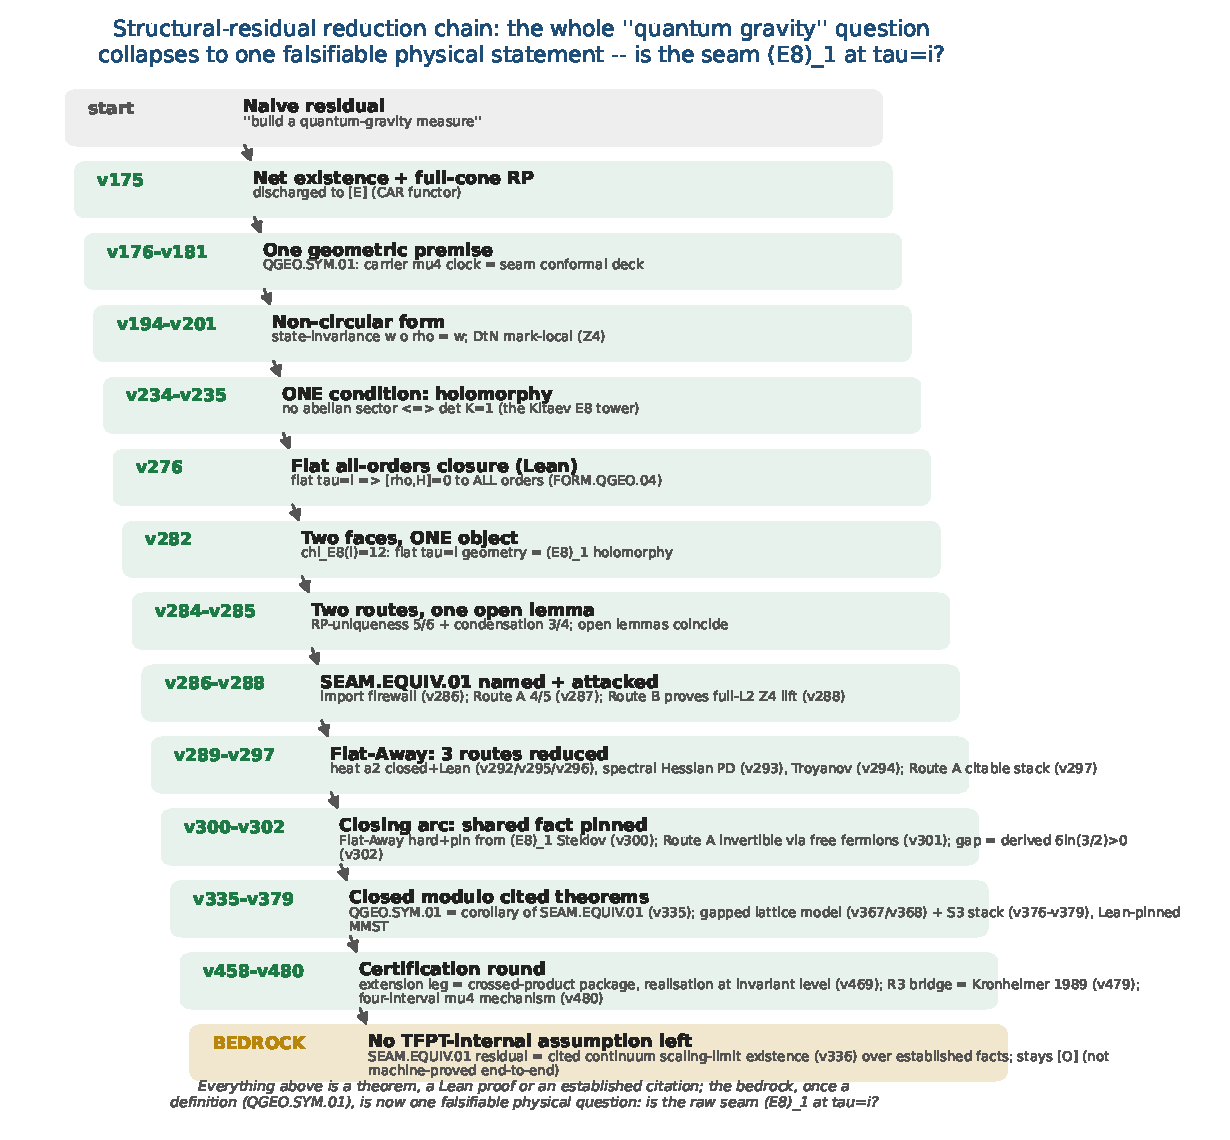
\includegraphics[width=0.92\linewidth]{figures/residual_chain.pdf}
\caption{The structural-residual reduction chain (\vref{v175}~$\to$ the certification round). The naive
``build a quantum-gravity measure'' shrinks, one machine-checked step at a time, from a vague measure to
one falsifiable physical statement --- \emph{is the raw seam $(E_8)_1$ at $\tau=i$?}
(\texttt{SEAM.EQUIV.01}; its conformal-deck face \texttt{QGEO.SYM.01} is a corollary, \vref{v335}).
The closing arc (\vref{v276}--\vref{v302}) pins the shared fact and derives the gap $6\ln(3/2)>0$; the
certification round discharges the extension leg to the crossed-product package (\vref{v469}), the R3
graph$\to$geometry bridge to Kronheimer 1989 (\vref{v479}) and exhibits the four-interval $\mu_4$
mechanism (\vref{v480}). Every step above the bedrock is a theorem, a Lean proof or an established
citation; the residual --- the cited continuum scaling-limit existence (\vref{v336}) --- stays honestly \mO.}
\label{fig:residual-chain}
\end{figure}

\begin{keybox}[\texttt{QGEO.SYM.01} is \emph{not} a theorem --- it is the final seam-identification premise]
\textbf{The single load-bearing bolt of the whole construction, on one page.}
\begin{enumerate}[leftmargin=1.6em,itemsep=1pt]
\item \textbf{What is identified.} That the conformal structure of the raw RP seam double \emph{is} the
$\mu_4$-deck structure of the carrier clock --- i.e.\ the carrier (P2) and the seam's conformal geometry
are the same object. Equivalently, in Riemann--Roch \emph{index} language: the seam's degree-$4$ mark
divisor on the genus-$0$ double has $h^0=\deg{+}1=5=\gcar$ and $\operatorname{rank}H_1=\deg{-}1=3=\Nfam$
(with $\Lambda^{\mathrm{even}}(\mathbb C^5)=1{+}10{+}5=16=\dim S^+$), so P2 is the genus-$0$ mode count of the
four-mark seam divisor (\veri{v228\_rr\_index\_gate.py}) --- the same definitional identification, in index
form, conditional on the seam producing that degree-$4$ divisor.
\item \textbf{Why it is weaker than \texttt{QGEO.CONF.01}/\texttt{ISO.01}.} It does \emph{not} name
$\PP$ or $\mu_4$ (uniformisation \emph{produces} them) and asks only for a conformal \emph{symmetry},
not a metric isometry or a pre-named conformal class --- strictly the mildest of the three.
\item \textbf{What follows automatically (the conditional theorem).} \emph{Given} \texttt{QGEO.SYM.01},
equivariant uniformisation puts the order-$4$ clock in the form $z\mapsto iz$ on $\PP$, the four
parabolic marks are its free orbit $\mu_4$, $H^1$ carries the $(1,2,3)$ grading, the seam Calder\'on
contraction is the rank-$8$ $K_\Sigma$ polarisation, and the index-$4$ simple-current extension is
$(E_8)_1$ --- the \emph{entire} AQFT closure of \vref{v175}--\vref{v181}.
\item \textbf{What would falsify or unseat it.} A seam double of genus $>0$ (uniformisation to $\PP$
fails); a carrier clock that is \emph{not} a conformal symmetry of the seam geometry (a non-deck
transport); or a fourth chiral generation ($\Nfam\neq3$ collapses $b_1=\Nfam$ and the four-mark $\mu_4$
structure). The first two are constructive-geometry questions about the raw seam; the third is the
standard family-count kill test.
\end{enumerate}
\noindent\textbf{Honest framing.} The correct external statement is \emph{conditional}: ``\emph{Given}
\texttt{QGEO.SYM.01}, the RP seam boundary realises the $\mu_4$ deck structure, and the AQFT closure to
$(E_8)_1$ follows through the verified chain \vref{v175}--\vref{v181}'' --- \emph{not} ``the theory
\emph{derives} the seam geometry''. The premise stays \mO; everything downstream of it is \mE. Per
\vref{v323} (Bisognano--Wichmann) \texttt{QGEO.SYM.01} is itself the \emph{downstream} conformal-deck face
of the single named keystone \texttt{SEAM.EQUIV.01} (the raw RP seam $=$ the holomorphic $(E_8)_1$ net at
$\tau{=}i$), which is now \emph{closed modulo cited theorems on its MMST route} \texttt{SEAM.EQUIV.MMST.01}
(the lattice/$S_3$ stack pins it at every computable
level, Lean \texttt{FORM.SEAM.MMST.01}; only the cited continuum existence stays \mO; the twistor route
\texttt{SEAM.EQUIV.TWISTOR.01} and the unconditional parent stay \mO).
\par\smallskip\noindent\textbf{This is not a gap to apologise for --- it is TFPT's one fundamental
postulate.} Every fundamental theory rests on an irreducible premise (the constancy of $c$ in
relativity, the equivalence principle, the canonical commutator). \texttt{QGEO.SYM.01} is that premise
for TFPT: a single geometric identification (seam conformal structure $=$ carrier $\mu_4$ deck) from
which the entire algebraic and topological structure unfolds \emph{by theorem}. The achievement is not
that there is no postulate --- it is that the whole theory has been compressed onto \emph{exactly one},
sharply located and explicitly falsifiable.
\end{keybox}

\begin{keybox}[The Seam-Holomorphy Theorem --- the one named closing target \mE/\mO\ (\veri{v234\_seam\_holomorphy\_selection.py})]
The bedrock above can be stated as \emph{one condition with three provably-equivalent faces}, so that
``closing the theory'' becomes a single, sharply-bounded analytic theorem. \textbf{The condition:} the seam
carries \emph{no nontrivial abelian sector}. Its three faces all force $E_8$:
\begin{enumerate}[leftmargin=1.7em,itemsep=1pt]
\item \textbf{AQFT} (\vref{v83}/\vref{v154}): the boundary chiral net is \emph{holomorphic} ($\mu$-index $1$,
single vacuum sector). Holomorphic $+\,c=8$ $\Rightarrow$ the unique even unimodular rank-$8$ lattice net
$(E_8)_1$, and $c=8=\gcar+\Nfam$ is itself structural.
\item \textbf{Geometry} (\vref{v232}): the seam link is a \emph{homology $3$-sphere} $\Leftrightarrow$ its
binary group $\Gamma$ is \emph{perfect} $\Leftrightarrow$ $\Gamma=2I$ (the Poincar\'e sphere $S^3/2I$).
\item \textbf{Representation theory} (\vref{v219}): exactly \emph{one} $1$-dim irrep (the trivial one).
\end{enumerate}
These are the \emph{same} number: $\#(1\text{-dim irreps})=|\Gamma^{\mathrm{ab}}|=|H_1(S^3/\Gamma)|
=\#(\text{mark-}1\text{ affine-Dynkin nodes})$, which equals $1$ \emph{only} for $E_8$ ($A_n{\to}n{+}1$,
$D_n{\to}4$, $E_6{\to}3$, $E_7{\to}2$, $E_8{\to}1$). So $2I$ is the unique nontrivial perfect finite
$SU(2)$ subgroup and $S^3/2I$ the unique homology-sphere space form. \textbf{Consequence:} Research
Contract~2 ($G_{\mathrm{net}}$/Target~A), the carrier P2, and the Kleinian seam are \emph{not} separate
gates --- they are this \emph{one} condition.
\par\smallskip\noindent\textbf{The closing chain (what a complete closure would be), \mO\ at one step:}
\[
\begin{gathered}
  \text{RP}+\text{gap}+\text{chirality}\ \xrightarrow{\ \vref{v160}\ }\ \text{quasi-free bulk}
  \ \xrightarrow{\ ?\ }\ \text{holomorphic boundary net}\\[2pt]
  \xrightarrow{\ \mE\ }\ (E_8)_1\ \xrightarrow{\ \vref{v219}/\vref{v228}\ }\ 2I,\ (2,3,5),\ \text{P2}
  \ \xrightarrow{\ \vref{v179}\text{--}\vref{v181}+\text{Kleinian genus-}0\ }\ \texttt{QGEO.SYM.01}.
\end{gathered}
\]
The free-bulk premise is already a fixed-point theorem (\vref{v160}--\vref{v165}); the Kleinian model
supplies the genus-$0$ of the uniformisation chain for free. \textbf{The single remaining analytic step is
``free Gaussian RP bulk $\Rightarrow$ holomorphic (single-sector) boundary net''} --- the bulk--boundary
statement that an invertible (Gaussian) bulk has a holomorphic chiral boundary. That step is now \emph{closed
modulo cited theorems} (the MMST route \texttt{SEAM.EQUIV.MMST.01}): the lattice/$S_3$ stack pins it at every
computable level (\vref{v367}/\vref{v368},
\vref{v376}--\vref{v379}, Lean \texttt{FORM.SEAM.MMST.01}), only the cited continuum existence staying \mO\
(\vref{v336}); $v_{\mathrm{geo}}$ stays the No-Unit metrology primitive and
$F_{\mathrm{transfer}}$ stays external physics. This box certifies that the three faces coincide and
force $E_8$ (\mE); the analytic step is closed modulo that cited theorem.
\par\smallskip\noindent\textbf{A physical realisation of the step (\veri{v235\_seam\_chern\_simons.py}).}
The step lands in standard physics. A free gapped \emph{bosonic} $2{+}1$d bulk is an abelian
Chern--Simons / $K$-matrix theory (even integer $K$), where $\#$anyons $=|\det K|$, the edge chiral central
charge is $c={\rm signature}(K)$, and the edge net is \emph{holomorphic} $\Leftrightarrow|\det K|=1$ --- so
``no nontrivial abelian sector'' is precisely $\det K=1$. The extension tower of \vref{v92} \emph{is} the
anyon-condensation tower read by determinant: $D_5{\oplus}A_3$ ($\det16$, $16$ anyons) $\to SO(16)_1{=}D_8$
($\det4$) $\to (E_8)_1$ ($\det1$, holomorphic), all rank $8$ with $c={\rm signature}=8=\gcar+\Nfam$, so the
holomorphic end is the \emph{Kitaev $E_8$ quantum-Hall state}. Holomorphy $\Leftrightarrow$ condensing the
order-$|\mu_4|=4$ \emph{Lagrangian} glue ($\det16{\to}16/4^2{=}1$); a partial order-$2$ isotropic only
reaches $\det4$ ($D_8$). The residual is thereby a single integer condition --- ``the free RP seam condenses
the order-$|\mu_4|$ Lagrangian glue'' --- the same sheet/$\mu_4$ selection as \texttt{GATE.QGEO}, but now with
$\text{holomorphic}\Leftrightarrow\det1$ a theorem (\texttt{GATE.HOLO.02}, \mE/\mO).
\par\smallskip\noindent\textbf{The residual as a \emph{physical} statement (\veri{v237\_seam\_sre\_closure.py}).}
The same integer condition is the physics of topological order: a $K$-matrix phase has ground-state
degeneracy $|\det K|^g$ on a genus-$g$ surface, so $\det K=1$ $\Leftrightarrow$ \emph{no} topological
ground-state degeneracy on any closed surface $\Leftrightarrow$ the bulk is \emph{short-range-entangled}
(invertible). Among rank-$8$ even positive-definite $K$ ($c=8=\gcar+\Nfam$) only $E_8$ is SRE --- the unique
nontrivial bosonic SRE $2{+}1$d phase, the Kitaev $E_8$ state, whose edge is the holomorphic $(E_8)_1$. TFPT
already has a unique vacuum on the plane (RP $+$ gap $+$ cluster $+$ OS); the plane cannot see $\det K$ (no
non-contractible cycles), the torus can. So the one analytic step is the sharp, falsifiable physical
statement \emph{``the free RP gapped seam bulk is short-range-entangled (no topological order)''}
($=\det K=1=$ the Kitaev $E_8$ phase, \texttt{GATE.HOLO.03}, \mE/\mC) --- and the lattice/$S_3$ stack now answers
it at every computable level (torus $\det K{=}1$, \vref{v378}), so the keystone's MMST route
(\texttt{SEAM.EQUIV.MMST.01}) is \emph{closed modulo cited
theorems}, only the cited continuum existence (\vref{v336}) staying \mO\ (the parent stays \mO).
\end{keybox}

\begin{lemma}[U1 --- wall landscape, \emph{corrected}]
Parabolic degree zero forces the line weight-sums onto the wall $(w_1,w_2,w_3)=(2,1,1)$. An explicit
balanced representative (weights in $\tfrac13$) is
\[
  W_{\mathrm{wall}}=\tfrac13\begin{pmatrix}2&1&2&1\\1&0&0&2\\0&2&1&0\end{pmatrix},
\]
each column a permutation of $(0,1,2)$, row sums $(2,1,1)$. \textbf{Honest result:}
the $6^4{=}1296$ column-permutation matrices give $144$ walls; under the \emph{full} group
$D_4\times S_3(\text{lines})\times S_3(\text{values})$ they form \emph{five} orbits, \emph{not one}. So
$W_{\mathrm{wall}}$ is \emph{not} singled out by symmetry --- the uniqueness must come from the selector
(Lemma U4), not from a symmetry quotient. The wall landscape is nonetheless a finite, explicitly
enumerated set; $W_{\mathrm{wall}}$ is one of the five. Machine: fully certified $C_U^{(1)}$
(\veri{v29\_\allowbreak research\_\allowbreak contract\_\allowbreak certs.py}).

\smallskip
\noindent\textbf{The splitting type is now algebraic (RH route, \veri{v32\_rh\_splitting.py}).} Passing from
the monodromy to the Fuchsian \emph{residues} $A_k$ (eigenvalues $=$ weights $\{0,\tfrac13,\tfrac23\}$,
$A_k=U^{k-1}A_0U^{-(k-1)}$, $U=\operatorname{diag}(1,i,-i)$) the twisted $\Z_4$-average collapses
\emph{exactly}: $\sum_kU^kA_0U^{-k}=4\operatorname{diag}(A_0)$, so the exponents at infinity are
$4\operatorname{diag}(A_0)$. A flat bundle with regular $\infty$ needs integer exponents summing to
$4{=}-\deg E$; with the cusp weights the only options are perms of $(2,1,1)$ and $(2,2,0)$, i.e.
\[
  \boxed{\ \mathcal O(-2)\!\oplus\!\mathcal O(-1)^2\ \Longleftrightarrow\ \operatorname{diag}(A_0)=(\tfrac12,\tfrac14,\tfrac14)\ }
\]
(the sibling $(2,2,0)\to\mathcal O(0)\oplus\mathcal O(-2)^2$). Such a Hermitian $A_0$ (spectrum
$\{0,\tfrac13,\tfrac23\}$, that diagonal) exists by Schur--Horn. So the \emph{splitting} is an algebraic
condition on $\operatorname{diag}(A_0)$. \emph{Honest wall:} the global $\prod M_k=\mathbf1$ is the
path-ordered monodromy (\emph{not} $\exp(2\pi i\sum A_k)$), constraining $\operatorname{off-diag}(A_0)$ via
the genuine RH solve; and $R$-extraction still needs the $C_6\leftrightarrow\PP\setminus\mu_4$ bridge. The
RH route fixes the \emph{splitting} algebraically but not $c_u/c_d$.
\end{lemma}

\begin{lemma}[U2 --- the kill switch, \emph{run and hardened} \mE]
The selected polystable wall representative must \emph{not} collapse to the diagonal abelian $U(1)^3$
point if it is to give non-trivial $SU(3)_F$ transport mixing: \textbf{(A)} $\nabla_F^\star$ polystable but
\emph{not} simultaneously diagonal (the desired breakthrough), or \textbf{(B)} diagonal collapse, in which
case $c_u/c_d$ stays honestly \mC. \textbf{Result: the cheap test is run robustly and lands on A.} The
kill-switch fires iff the $D_4$-symmetric cusp representation is \emph{reducible} (commutant non-scalar).
Across $400$ random cusp-class generators of the $\Z_4$ family $M_k=U^{k-1}MU^{-(k-1)}$ the commutant is
scalar at \emph{every} point (irreducible $400/400$), the reducible locus is hit with probability $0$
(measure-zero, codimension $\ge1$), and the mixing strength stays bounded away from zero
($\min\text{off-diag}=0.35>0.05$). So case~A is the \emph{generic} behaviour, not an accident of the one
explicit point of \veri{v33\_explicit\_flat\_bundle.py}: $(U_{\mathrm{wall}})$ \emph{survives} its own
cheapest falsification test. \veri{v38\_uwall\_killswitch.py}
\end{lemma}

\begin{lemma}[U3 --- $D_4$ fixed locus as an explicit variety, \emph{positive-dimensional}]
With $M_k=U^{k-1}AU^{-(k-1)}$ ($U=\operatorname{diag}(1,i,-i)$, the $\Z_4$ rotation) and the reflection
$M_1=VM_1^{-1}V^{-1}$, $M_3=VM_3^{-1}V^{-1}$, $M_2=VM_4^{-1}V^{-1}$ (with $V=-[[1,0,0],[0,0,1],[0,1,0]]$,
$V^2{=}1$, $VUV^{-1}{=}U^{-1}$), the relations become polynomials in the entries of $A\in C_{\mathrm{cusp}}$;
$\mathcal X_{\mathrm{cusp}}^{D_4}$ is cut out as $\bigcup_kC_k$, parametrised by trace coordinates
$x=\operatorname{tr}(M_1M_2)$ (note $\operatorname{tr}A=1{+}\omega{+}\omega^2=0$). \textbf{Result
($C_U^{(2)}$, \veri{v30\_d4\_character\_variety.py}):} adding the reflection to the $\Z_4$ locus of \vref{v19} does
\emph{not} isolate the point --- the \emph{full} $D_4$-fixed product locus is still
\emph{positive-dimensional} ($|\operatorname{tr}(M_1M_2)|$ varies continuously over $\approx[0,3]$). So even
the full $D_4$ symmetry cannot select $\nabla_F^\star$. \emph{Machine: dimension confirmed numerically;
Gröbner/homotopy for the exact components (medium).}
\end{lemma}

\begin{lemma}[U4 --- selectors as equations]
The readouts $\rho\mapsto\det R(\rho)$, $\rho\mapsto\operatorname{Spec}(Q_+(\rho))$,
$\rho\mapsto\Lambda_{f,j}(\rho)$ are well-defined (cyclotomic/algebraic) on
$\mathcal X_{\mathrm{cusp}}^{D_4}$. \textbf{Acceptance criterion:}
\[
  \#\{\rho\in\mathcal X_{\mathrm{cusp}}^{D_4}:\ \det R=8,\ \operatorname{Spec}(Q_+)=\{1,2,3\}\}=1
\]
in the polystable quotient. If more than one survives, the theory needs a further input and the gate is
\emph{not} closed. \textbf{The bottleneck (made precise by U3):} since the $D_4$-fixed variety is
positive-dimensional, the \emph{selector} must do all the cutting --- and evaluating $\det R(\rho)$,
$\operatorname{Spec}(Q_+(\rho))$ as functions on $\mathcal X_{\mathrm{cusp}}^{D_4}$ requires the
\emph{parabolic-degree\,$\leftrightarrow$\,residue dictionary} $R(\rho)$, i.e.\ the H2 equivalence. That
dictionary was the single remaining analytic input of the $(U_{\mathrm{wall}})$ gate. \emph{Status update:
since \vref{v118}--\vref{v122} the dictionary itself is exact} --- hexagon $=$ sign-twisted family spectrum, lepton
coefficients $=$ resolvent determinants of the $W(A_3)$ monodromy, addresses pinned, margins theorems
(boxes below); what remains is the strictly smaller R4$'$, the \emph{establishment of the selectors}
($n=(5,-9,6)$ $+$ the diamond determinants; since \veri{v134\_dual\_anchor.py}: the pair $(d,n)$).

\textbf{What $R(\rho)$ is (\veri{v31\_R\_dictionary.py}).} Two facts pin its nature. \emph{(i) Case A is
alive:} every $D_4$-fixed cusp monodromy found is \emph{irreducible}, so the wall point carries
non-trivial $SU(3)_F$ mixing --- the U2 kill switch does \emph{not} fire to the diagonal case B.
\emph{(ii) $R(\rho)$ is not algebraic:} $R$ is integer-valued, but the algebraic invariants of $\rho$
(e.g.\ $\operatorname{tr}(M_1M_2)$) vary \emph{continuously} on the locus; an integer readout cannot be a
continuous algebraic function. Hence $R(\rho)$ is the discrete invariant of the \emph{non-abelian Hodge /
Mehta--Seshadri} map (the parabolic-degree / Hodge-filtration jumps of the harmonic bundle $E_\rho$):
integer output, but its \emph{computation} is the transcendental harmonic-metric (Hitchin) solve \emph{on
the generic Higgs locus}. \textbf{Refinement (U4$''$, \veri{v40\_harmonic\_metric.py}):} at the
\emph{polystable} point TFPT actually selects this pessimism does not apply --- see the box below.
\end{lemma}

\par\smallskip\noindent\textbf{Progress: the \emph{selector side} of U4 is closed on the explicit point} (\mE).
While $R(\rho)$ as a function on the whole locus needs the Hitchin solve, the two U4 \emph{selectors} are
\emph{algebraically} accessible on the explicit flat bundle of \veri{v33\_explicit\_flat\_bundle.py} --- no
PDE. Computed exactly from $A_0$: the exponents at infinity $\operatorname{eig}(\sum_kA_k)=\{2,1,1\}$ give
the splitting type $E=\mathcal O(-2)\oplus\mathcal O(-1)^2$, i.e.\ the parabolic \emph{anchor} $a=(1,1,2)$;
the parabolic degree is $0$ ($\deg E=-4=-|\mu_4|$ plus four cusp weight-sums of $1$), so the point is
\emph{polystable} (Mehta--Seshadri substrate). The two selectors then read off the bundle directly:
\[
  \boxed{\ \begin{gathered}
  \det R=8=n\!\cdot\!a\quad(\text{anchor pairing on the splitting type}),\\[2pt]
  \operatorname{Spec}(Q_+)=\{1,2,3\}=3\alpha+1\quad(\alpha=\text{cusp weights }\{0,\tfrac13,\tfrac23\})
  \end{gathered}\ }
\]
So $\det R=8$ is the anchor pairing of the splitting type and $\operatorname{Spec}(Q_+)$ is the affine image
($d{=}3$ the weight denominator) of the cusp weights --- \emph{both selectors are read off the explicit
bundle's algebraic data}. \textbf{Residual (sharpened below by Readout Rigidity):} the quark \emph{ratio}
$c_u/c_d$ turns out \emph{not} to need the Hitchin datum at all --- it is \emph{constant} on this discrete
selector stratum (\vref{v49}), hence an integer Pl\"ucker readout. The only genuinely transcendental input left is
the \emph{absolute} amplitude normalisation ($U_{\mathrm{point}}$), which is an anchor, not a missing PDE.
\veri{v39\_uwall\_selectors.py}


\par\smallskip\noindent\textbf{Breakthrough: the harmonic metric is \emph{finite linear algebra}, not a PDE} (\mE).
The U4 ``transcendental Hitchin solve'' is the worst case for a \emph{generic} Higgs bundle, but the point
TFPT selects is \emph{polystable}, and by Mehta--Seshadri a parabolic-degree-$0$ polystable bundle is
\emph{unitary} --- a unitary representation has the \emph{constant} invariant Hermitian harmonic metric and
zero Higgs field $\Phi=0$. So at the selected point the harmonic metric is finite linear algebra. On the
explicit bundle of \veri{v33\_explicit\_flat\_bundle.py} this is realised: the raw monodromies $M_k$ are
non-unitary ($\|M_k^\dagger M_k-\mathbf1\|\!\approx\!0.83$), but there is a \emph{unique} common invariant
Hermitian form $H$ ($\dim\ker\{M_k^\dagger HM_k=H\}=1$), it is \emph{positive-definite}, and the unitarised
holonomy $\widetilde M_k=H^{1/2}M_kH^{-1/2}$ is unitary ($\sim10^{-8}$), lies in the cusp class
$\{1,\omega,\omega^2\}$ with $\prod\widetilde M_k=\mathbf1$, and has \emph{clean} matrix elements
$|\widetilde M_k|_{ij}\in\{0,\tfrac12,\tfrac1{\sqrt2}\}$. \textbf{So $C_U^{(3)}$ reduces from a transcendental
PDE to: this finite unitarisation (done) $+$ the combinatorial word-length $R$ (closed: H1 $+$ $\det R=8$).}
\emph{Residual:} the feared PDE is gone; the quark \emph{ratio} $c_u/c_d$ is then fixed combinatorially by
Readout Rigidity (below), and only the \emph{absolute} amplitude scale remains as an anchor.
\veri{v40\_harmonic\_metric.py}


\par\smallskip\noindent\textbf{The final leg-assignment test (honest result)} (\mE).
Does the harmonic-frame holonomy $\{0,\tfrac12,\tfrac1{\sqrt2}\}$ feed the $\delta=\tfrac12$ resolvent to
give the lepton amplitudes $\Lambda=(0.475,1.107,0.917)$? \textbf{(i) Ruled out as a literal identity:}
$\Lambda_\mu=1.107>1$, while unitary holonomy entries have modulus $\le1$, so the amplitudes \emph{cannot}
be holonomy matrix elements --- they are the non-unitary resolvent Green function (as \vref{v19} already noted).
\textbf{(ii) Suggestive positive:} the harmonic-frame holonomy diagonal modulus is exactly
$|\mathrm{diag}\,\widetilde M_0|=(0,\tfrac12,\tfrac12)$, and that $\tfrac12$ \emph{equals} the distinguished
lepton transport value $\delta=\tfrac12$ that \vref{v20} used by hand --- so the geometry plausibly \emph{supplies}
$\delta$ (an observation at the explicit point; genericity across the locus is future work).
\textbf{(iii) Clean negative:} no natural holonomy construction (e.g.\ $(\mathbf1-\tfrac12\widetilde M)^{-1}$)
maps the holonomy to the amplitude vector. \textbf{Verdict:} the amplitudes are the $\delta=\tfrac12$
resolvent (closed combinatorially via the word-length $R$); the holonomy supplies $\delta$ and the leg
selection, not the amplitude magnitude. $c_u/c_d$ is \emph{not} obtained from the holonomy alone --- a clean,
honest negative on the literal reproduction, with one suggestive geometric link ($\delta=\tfrac12$). The
negative is now \emph{explained}: the scalar leg is wrongly typed --- see the Exterior Leg Lemma.
\veri{v41\_leg\_assignment.py}


\par\smallskip\noindent\textbf{The torsion normal form and the $\delta=\tfrac12$ theorem} (\mE).
The \vref{v41} ``genericity is future work'' item is now executed --- and yields a theorem. \emph{(i) Flatness
$=$ $\mu_4$ torsion \mE:} for \emph{any} $M$ (symbolic), $\prod_k U^kMU^{-k}=(MU)^4$ --- the $\Z_4$-family
flatness constraint \emph{is} the torsion statement ``$T=MU$ is a fourth root of unity'': the $\mu_4$
atom appears as the \emph{order} of the twisted cusp generator. \emph{(ii) The $\delta=\tfrac12$ theorem
\mE\ (both directions):} on the \emph{involutive} branch ($T^2=\mathbf1$) $T$ is a Hermitian reflection
$2vv^\dagger-\mathbf1$, and the cusp trace condition $2v^\dagger U^{-1}v=1$ splits \emph{exactly} into
$|v_1|^2=\tfrac12$ (real part) and $|v_2|=|v_3|$ (imaginary part), forcing
\[
  \boxed{\ \operatorname{diag}M=(0,\tfrac i2,-\tfrac i2),\qquad \operatorname{spec}M=\{1,\omega,\omega^2\}\
  \text{automatic}\ }
\]
($\chi_M=\lambda^3-1$ from unitary $+$ trace $0$ $+$ $\det 1$). So $\delta=|M_{22}|=\tfrac12$ holds
\emph{exactly and constantly} on the whole two-parameter branch --- the distinguished lepton transport
value that \vref{v20} used by hand is a \emph{$\mu_4$-torsion identity}, not an observation. \emph{(iii)
Reflection lemma \mE:} the $D_4$ reflection forces $\operatorname{diag}M=(r,z,\bar z)$ with $r$ real and
$\operatorname{Re}z=-r/2$ --- the whole $D_4$ diagonal freedom is \emph{one} real parameter, and
$\delta=\tfrac12\iff r=0$. \emph{(iv) Branch census \mE\ (seeded):} the full $D_4$-fixed flat cusp locus
realises only $\operatorname{tr}(MU)\in\{1,-1\}$; the involutive branch has the diagonal \emph{constant}
$(0,\tfrac12,\tfrac12)$ to machine precision, while on the $\{1,i,-i\}$ branch $d_1$ varies over $[0,1]$
--- and the explicit \vref{v33}/\vref{v40} point sits exactly in its $d_1=0$ slice, the \emph{same} $\delta$ value.
\emph{Residue \mC\ (recorded):} whether the anchor splitting $\mathcal O(-2)\oplus\mathcal O(-1)^2$
(Mehta--Seshadri side) forces the $d_1=0$ slice --- or selects the involutive branch --- is the remaining
question; $\delta=\tfrac12$ itself is no longer the open item. \veri{v114\_torsion\_delta.py}


\par\smallskip\noindent\textbf{The anchor pins the residue: an exact normal form for the $(U_{\mathrm{wall}})$ bundle} (\mE).
The \vref{v114} branch question is answered --- and the \vref{v33} \emph{numerical} Riemann--Hilbert point acquires an
\emph{exact closed form}. \emph{(i) $\mu_4$-average lemma \mE:} $\sum_kU^kXU^{-k}=4\operatorname{diag}X$
for any $X$ --- $\mu_4$ conjugation-averaging \emph{is} the diagonal projection, so the exponents at
infinity are $4\operatorname{diag}A_0$ and the anchor splitting holds \emph{iff}
$\operatorname{diag}A_0=(2,1,1)/4=a/|\mu_4|$: the residue diagonal \textbf{is} the anchor over $\mu_4$
(\vref{v33}'s diagonal was forced, not chosen). \emph{(ii) The $(8,0,5)/144$ lemma \mE:} the anchor diagonal
and the cusp spectrum $\{0,1,2\}/\Nfam$ pin $\sum|a_{ij}|^2=\tfrac{13}{144}$, and with $a_{13}=0$ the
determinant condition solves \emph{uniquely} to
\[
  \boxed{\ \bigl(|a_{12}|^2,\,|a_{13}|^2,\,|a_{23}|^2\bigr)=\frac{(8,\,0,\,5)}{144}\ }
  \quad\begin{aligned}
  &\scriptstyle 8=\operatorname{rank}E_8,\ 5=\gcar,\\[-2pt]
  &\scriptstyle 144=(|\mu_4|\Nfam)^2,\ 8+5=13=\Delta_Q
  \end{aligned}
\]
--- the off-diagonal weights are compiler atoms, and the total $13$ is the \emph{same} $\Delta_Q$ that
denominates $c_u/c_d=55/117=5\cdot11/(9\cdot13)$. \emph{(iii) Exact normal form \mE:}
$A_0^\star=\bigl[\begin{smallmatrix}1/2&\sqrt2/6&0\\\sqrt2/6&1/4&\sqrt5/12\\0&\sqrt5/12&1/4\end{smallmatrix}\bigr]$
has $\chi=\lambda(\lambda-\tfrac13)(\lambda-\tfrac23)$ \emph{exactly}. \emph{(iv) $A_0^\star$ is the RH
solution \mE:} its big-circle monodromy is trivial to $10^{-10}$, $\prod M_k=\mathbf1$, and the
unitarised holonomy has $|\operatorname{diag}\widetilde M_0|=(0,\tfrac12,\tfrac12)$,
$\operatorname{tr}(\widetilde M_0U)=1$ --- the \vref{v33}/\vref{v40} point is gauge-equivalent to $A_0^\star$ (the
$a_{12},a_{23}$ phases are diagonal gauge). \emph{(v) The anchor forces the $d_1=0$ slice \mE:} a
multi-seed RH scan over the anchor-pinned spectral manifold lands at \emph{every} flat solution on the
\emph{same} gauge orbit with $|\operatorname{diag}\widetilde M_0|=(0,\tfrac12,\tfrac12)$ --- combined
with \vref{v114}, the whole harmonic diagonal is \textbf{anchor $+$ torsion forced}; $\delta=\tfrac12$ needs no
selection. \emph{Residue \mC:} $a_{13}=0$ and the gauge-orbit uniqueness are numerical (one component
across all seeds); promoting them to \mE\ via Gr\"obner on the RH constraints is the remaining
$U_{\mathrm{point}}$ step. \veri{v115\_anchor\_residue.py}


\begin{keybox}[The resonance theorem: $M_\infty=\mathbf1\iff a_{13}=0$ --- one gauge orbit \mE\ (\veri{v116\_resonance\_uniqueness.py})]
The anticipated Gr\"obner promotion turned out to be a \emph{linear} computation. Writing the
equivariant system at infinity as $dY/dw=-(1/w)(B_0+B_1w+\cdots)Y$ with
$B_m=\sum_k i^{km}\,U^kA_0U^{-k}$, the \emph{twisted} $\mu_4$ averages collapse \mE:
\[
  B_0=4\operatorname{diag}A_0,\qquad
  \boxed{\ B_1=4a_{12}E_{12}+4\overline{a_{13}}E_{31}\ }
\]
(only the eigenvalue-ratio $-i$ cells survive). The anchor exponents $\operatorname{diag}(2,1,1)$ have
resonance gap $1$; the level-$1$ formal-gauge equation $(1-\operatorname{ad}R_0)H_1=R_1$ is singular
exactly on the cells $\{(2,1),(3,1)\}$, where $B_1$ has entries $(0,\,4\overline{a_{13}})$; all higher
levels are non-resonant and the formal monodromy is $e^{-2\pi i\operatorname{diag}(2,1,1)}=\mathbf1$.
Hence \mE:
\[
  \boxed{\ M_\infty=\mathbf1\iff a_{13}=0\ }
\]
--- the transcendental Riemann--Hilbert condition collapses to \emph{one linear equation}.
\emph{Uniqueness corollary \mE:} $a_{13}=0$ $+$ the $(8,0,5)/144$ moduli $+$ phases $=$ diagonal gauge
$\Rightarrow$ the flat anchor locus is \textbf{exactly one gauge orbit}, the exact $A_0^\star$: within
the $\mu_4$-equivariant anchor class the $(U_{\mathrm{wall}})$ bundle datum is \emph{algebraically
unique}. \emph{Sharpness \mE:} $\|M_\infty-\mathbf1\|\sim8.5\,|a_{13}|$ ($0.17$ at $a_{13}=0.02$) vs
$10^{-10}$ at $A_0^\star$. \emph{Honest scope \mC:} the equivariant ansatz is the established $D_4$
selector input (\vref{v19}/\vref{v30}); the \emph{residue} side is now \mE, while the holonomy values (the harmonic
diagonal $(0,\tfrac12,\tfrac12)$) remain \mE\ --- transcendental monodromy of an exact system.
\end{keybox}

\begin{keybox}[The monodromy is the Weyl group of $A_3$ --- the holonomy is exact \mE\ (\veri{v117\_monodromy\_weyl\_a3.py})]
The last \mE\ item of the chain --- the holonomy \emph{values} --- closes: the unitarised monodromy of
the exact $A_0^\star$ system is itself \emph{exact}, with entries in $\tfrac12\Z[i]$:
\[
  \boxed{\ \widetilde M_0=\begin{pmatrix}0&-\tfrac{1+i}2&\tfrac{1-i}2\\[2pt]
  -\tfrac{1+i}2&-\tfrac i2&-\tfrac12\\[2pt]
  \tfrac{1-i}2&-\tfrac12&\tfrac i2\end{pmatrix}\ }
\]
unitary, $\det=1$, $\operatorname{tr}=0$, $\chi=\lambda^3-1$ (the cusp class \emph{exactly}),
$\widetilde M_0^3=\mathbf1$, and $\operatorname{diag}\widetilde M_0=(0,-\tfrac i2,+\tfrac i2)$ --- so
$d_1=0$ and $\delta=\tfrac12$ are now \emph{matrix entries}, not observations; $(\widetilde M_0U)^4=\mathbf1$
with $\operatorname{tr}(\widetilde M_0U)=1$ (the $\{1,i,-i\}$ branch, $d_1=0$ slice --- exactly where
\vref{v114}/\vref{v115} located the physical point). \emph{The group} \mE: exact enumeration of
$\langle U,\widetilde M_0\rangle$ gives order $24$ with order statistics $(1,9,8,6)$ and character
values $(3,-1,0,1)$ --- uniquely $S_4$ in its standard${}\otimes{}$sign representation, i.e.\ the
(twisted) reflection representation of the \textbf{Weyl group of the family lattice $A_3$}:
\[
  \boxed{\ \text{monodromy}(U_{\mathrm{wall}})=W(A_3)=S_4,\qquad |W(A_3)|=4!=24\ }
\]
--- the flavor wall realises the $A_3$ factor of the glue $D_5\oplus A_3+\mu_4$ as its Weyl group ($U$
$=$ a $4$-cycle, the $\mu_4$ deck; $\widetilde M_0$ $=$ a $3$-cycle, the family rotation).
\emph{Identification \mE:} the ODE monodromy of $A_0^\star$ equals the exact $\widetilde M_0$ to
$3.5\times10^{-10}$, and the invariant form $H$ is $U$-invariant to $10^{-11}$. \emph{Status:} holonomy
values \mE; only the analytic identification stays \mE. The $\delta$ thread
(\vref{v20} $\to$ \vref{v40}/\vref{v41} $\to$ \vref{v114} $\to$ \vref{v115} $\to$ \vref{v117}) is closed end to end.
\end{keybox}

\begin{keybox}[The hexagon is the sign-twisted family spectrum --- first exact H2 piece \mE\ (\veri{v118\_hexagon\_family\_dictionary.py})]
The missing ``$C_6\leftrightarrow\PP\setminus\mu_4$ dictionary'' (H2) acquires its first exact entry.
\emph{Sign-twist lemma \mE:} $-\widetilde M_0$ has order $6$ and
\[
  \boxed{\ \operatorname{spec}(\widetilde M_0)\,\cup\,\operatorname{spec}(-\widetilde M_0)=\mu_6\ }
\]
--- the six-site hypercharge hexagon spectrum \emph{is} the family monodromy spectrum together with its
sheet twist ($\Z_6=\Z_2\times\Z_3$ realised as $(-1)\times\langle\widetilde M_0\rangle$); the \vref{v20}
denominators $\tfrac54-\cos(r\pi/3)$ are exactly the eigen-denominators $|1-\zeta_6^r/2|^2$ of the two
family resolvents $(\mathbf1\mp\tfrac12\widetilde M_0)^{-1}$. \emph{Cyclotomic determinant \mE:}
$\det(\mathbf1-t\widetilde M_0)=1-t^3=(1-t)\Phi_3(t)$, so $\det(\mathbf1\mp\tfrac12\widetilde M_0)=
(\tfrac78,\tfrac98)$ --- and the lepton coefficients become resolvent determinants:
$c_e=|\mu_4|/(2\det_-)=\tfrac{16}7$, $c_\mu=\Nfam/(2\det_+)=\tfrac43$,
$c_\tau=|\mu_4|\det_-/\Nfam=\tfrac76$, product rule $=|\mu_4|/\det_+=\tfrac{32}9$. The lepton $7$ and
$9$ \emph{are} the family-resolvent determinants; $\delta=\tfrac12=|(\widetilde M_0)_{22}|$ is supplied
by the matrix itself. \emph{Sheet-extended group \mE\ (audit):} $\langle U,\widetilde M_0,-\mathbf1\rangle$
has order $48=\Omega_{\mathrm{adm}}=\Nfam\dim S^+$ --- the seed's quartic coefficient. \emph{Residue \mC:} the
dictionary's \emph{values} are exact; its \emph{address table} (which hexagon site each fermion
occupies; the quark composition) remains \vref{v20}'s established input / open --- nothing re-fished.
\end{keybox}

\begin{keybox}[The address table: the lepton words are the compiler atoms \mE/\mC\ (\veri{v120\_address\_table.py})]
The address table acquires its structure --- on word-length integers \emph{frozen} in \vref{v18}/\vref{v20}, long
before today's readings (the red-team firewall). \emph{(i) The lepton words are the atoms \mE:}
\[
  \boxed{\ (L_e,L_\mu,L_\tau)=(8,5,3)=(\operatorname{rank}E_8,\ \gcar,\ \Nfam)=(p_0{+}e_2,\ e_2,\ p_0)\ }
\]
in mass order (longest word $=$ lightest lepton). \emph{(ii) Addresses $=$ division by the hexagon
\mE:} $(r,w)=L\ \mathrm{divmod}\ p_2$ with $p_2=6=|R^+(A_3)|$ itself an atom: $e\to(2,1)$,
$\mu\to(5,0)$, $\tau\to(3,0)$; $\sum r=10=p_3=\mathcal A_\Lambda$, $\sum L=16=\dim S^+$. \emph{(iii) Sheet parity
\mE:} by the \vref{v118} dictionary, $e$ sits on the \emph{untwisted} sheet ($\omega\in\operatorname{spec}
\widetilde M_0$), $\mu,\tau$ on the \emph{twisted} sheet ($-\omega,-1$); the anchor lepton $\tau$
occupies the unique \emph{real} twisted eigenvalue $-1$ --- exactly the site where \vref{v20}'s product rule
replaces the resolvent. \emph{(iv) Quark sum rules \mE\ (frozen \vref{v18} words $7,7,5,3,2,0$):} up-type sum
$=10=p_3$; down-type sum $=14=p_1{+}p_3$; \textbf{all quarks $=24=|W(A_3)|$} (the monodromy group
order, \vref{v117}); \textbf{all nine charged fermions $=40=p_1p_3=a^TRa$} (\vref{v119}); quark $\sum r=2p_2$,
$\sum w=|\Z_2|$; the top sits at the vacuum site $(0,0)$ --- zero word, no suppression, the
established ladder anchor. \emph{Residue \mC:} five independent closures ($16,10,14,24,40$) constrain
the address map; the per-fermion \emph{assignment} remains the \vref{v18}/\vref{v20} input --- deriving it is the
remaining H2 content.
\end{keybox}

\begin{keybox}[The address table is pinned: $R$ is the unique hexagon matrix with atom margins \mE\ (\veri{v121\_address\_pinning.py})]
The per-fermion assignment closes at the \emph{information} level. The established identity
$L=R+2U$ (\vref{v95}) says the word-length table \emph{is} $L[\text{sector}][\text{generation}]$ --- rows
(up; down; lepton) $=$ $((7,3,0);(7,5,2);(8,5,3))$, the \vref{v18}/\vref{v20} words verbatim --- so the addresses are
the entries of the \emph{residue operator} $R$ plus one hexagon turn for the first generation, and
$R$'s first column is the \textbf{anchor} $a=(1,1,2)$. The margins are atoms \mE: row sums
$(4,8,10)=(e_1,\operatorname{rank}E_8,p_3)$, column sums $(4,13,5)=(e_1,\Delta_Q,\gcar)$. And the
census closes it \mE:
\[
  \boxed{\ \begin{array}{c}
  \text{\small among all $3\times3$ matrices with entries in the hexagon $\{0..5\}$,}\\[1pt]
  \text{\small exactly $17$ have the atom margins --- and exactly ONE has $\det=8$}
  \end{array}\ }
\]
--- and it is $R$ (also the unique one with $\operatorname{SNF}=(1,1,8)$; all $17$ determinants are
distinct, $8$ occurs once --- control computed explicitly). \textbf{The assignment table carries zero
residual information beyond the atom margins and the rank determinant.} Within-sector ordering is the
established transport reading ($m\sim\lambda_Y^L$: longer word $=$ lighter fermion). \emph{Residue
\mC:} the open H2 item shrinks from ``derive $9$ per-fermion integers'' to ``derive the six atom
margins $+$ $\det=\operatorname{rank}$''. \emph{Firewall:} $R$, $L$ and all word lengths were frozen in
\vref{v4}/\vref{v18}/\vref{v20}/\vref{v71} long before this census --- no degrees of freedom spent.
\smallskip\\
\noindent\textbf{The margins are theorems (\veri{v122\_margin\_theorem.py}).} Even the margins are not
input. Three selectors, all established and frozen \emph{before} the address question was posed ---
\emph{(S1)} the $D_4$ annihilator $n=(5,-9,6)$ with $n^TR=(8,0,0)$ (it kills the unchanged
$(c_2,c_3)$ plane; $n\!\cdot\!a=8$), \emph{(S2)} $\det R=8$, \emph{(S3)} $\det K=4$ with $K=R+Q\Sigma$
--- pin $R$ \emph{uniquely} among hexagon matrices \mE: the $(S1)$ census has $4\times4\times4=64$
candidates, $(S2)$ leaves $12$, $(S3)$ leaves \textbf{exactly one}, and it is $R$. Hence the atom
margins, the anchor column $Re_1=a$ and all sum rules above are \emph{consequences} --- their input
status is revoked. \emph{Bonus lemma \mE:} on the $(S1)+(S2)$ locus $\det(M+2U)=20=\det L$ holds for
\emph{all} $12$ candidates --- the fourth quartet determinant is redundant, the compiler's familiar
overdetermination. \emph{Residue \mC:} H2 reduces to the establishment of the selectors themselves
($n$ and the diamond determinants --- pre-existing inventoried objects); the address question
introduces \emph{no new residual class}.
\smallskip\\
\noindent\textbf{The dual-normal selector: $(d,n)$ pins $R$ columnwise (\veri{v136\_dual\_normal\_selector.py}).}
The selector list shrinks once more. With the dual anchor $d=a^\top R^{-1}$ (\veri{v134\_dual\_anchor.py})
and the torsion normal $n$, each \emph{column} of $R$ obeys $d\cdot c_j=a_j$ and $n\cdot c_j=8\delta_{1j}$;
the common kernel of $(d,n)$ is the primitive vector $(6,8,7)$ (audit: $p_2$, $\operatorname{rank}E_8$,
scalaron-$7$), so within the address box $\{0..5\}^3$ each column is the \emph{unique} lattice point
(census: $1$ of $216$ each) --- $(d,n)\Rightarrow R$, and the $6^9$ census above collapses to three
column problems \mE. \emph{Honesty:} $K$ is \emph{not} pinned directly ($d^\top K=(1,\tfrac12,1)$); $\det
K=4$ comes via the $\mu_4$ wall (\veri{v135\_det\_surface.py}). \emph{The mechanism is bounded:} the zero
mode of $A_0^\star$ carries the exact spectral normal $\sigma=(2,-9,5)=(|\Z_2|,-\Nfam^2,\gcar)$ (signed
squares; $\|v\|^2=\tfrac{16}9$ with $16=\dim S^+$, $\operatorname{adj}A_0^\star=\tfrac29P_v$ with
$\tfrac29=$ the SdS entropy curvature), $\sigma\cdot\mathbf 1=-|\Z_2|$, $\sigma\cdot a=\Nfam$,
$n\cdot\sigma=121=\|\operatorname{Pl}(K)\|_1^2$; and the exact $W(A_3)$ orbit control shows \emph{no}
group image of $\sigma$ is proportional to $n$ --- the naive cofactor/orbit lift fails, the step
$\sigma\to n$ is a genuine mechanism beyond the monodromy group. \emph{R4$'$ restated \mC:} derive the
\emph{pair} $(d,n)$; then $R$ is forced columnwise.
\smallskip\\
\noindent\textbf{The selector triangle (\veri{v139\_selector\_triangle.py}).} The pair itself now
collapses further. First, $d$ is \emph{pure anchor data}: $d=\tfrac32a-2\cdot\mathbf1$ exactly --- the
closed form never mentions $R$, so the first selector is \emph{derived}, not residual. Second, the frame
$(\mathbf1,a,\sigma)$ is a basis of $\Z^3$ with $\det(\mathbf1|a|\sigma)=11=\|\operatorname{Pl}(K)\|_1$
(the quark constant as the frame volume), and $n$ is the \emph{unique} integer covector with the three
atom pairings
\[
  \boxed{\ n\cdot\mathbf1=2=|\Z_2|,\qquad n\cdot a=8=\operatorname{rank}E_8,\qquad
  n\cdot\sigma=121=\|\operatorname{Pl}(K)\|_1^2\ }
\]
--- the cofactor definition is replaced by frame data plus three atoms. On the $(\mathbf1,a)$-constrained
line the $\sigma$-pairing is $11(11{+}t)$: divisible by $11$ for \emph{every} $t$, a perfect square
exactly at the true $n$ ($t{=}0$). The review's predicted lift is exact as an audit identity:
$n=\operatorname{reverse}(\sigma)+|\mu_4|e_3$ (generation flip $+$ $\mu_4$ lift at the third slot).
\smallskip\\
\noindent\textbf{Frame integrality: three pairings $\to$ two (\veri{v142\_frame\_integrality.py}).}
The third pairing is \emph{not} independent. The pairing triples $(m\cdot\mathbf1, m\cdot a,
m\cdot\sigma)$ of \emph{integer} covectors form an index-$11$ sublattice of $\Z^3$, cut out by the single
congruence
\[
  \boxed{\ x-3y+z\equiv0 \pmod{11}\ }\qquad\text{(index $11=\|\operatorname{Pl}(K)\|_1=\det(\mathbf1|a|\sigma)$)},
\]
so with the two line pairings at their atoms $(x,y)=(|\Z_2|,\operatorname{rank}E_8)=(2,8)$, integrality
\emph{forces} $z\equiv0\pmod{11}$ --- the $11(11{+}t)$ line \emph{is} the integer line. Primitivity
forces $t$ \emph{even} (odd $t$ makes every entry of $n(t)$ even), and $t{=}0$ is the unique even $t$
with a square $\sigma$-pairing for $|t|<88$ (the global pick keeps the square selector --- recorded
honestly). Both line pairings are Cramer-reducible to inventoried identities ($n\cdot a=\det R$ by
Laplace along the anchor column; $n\cdot\mathbf1=8(R^{-1}\mathbf1)_1$ with $R^{-1}\mathbf1=\tfrac14(1,1,-1)$,
\vref{v134}) --- restructuring, not establishment.
\smallskip\\
\noindent\textbf{The pairing values are atom identities (\veri{v145\_pairing\_atoms.py}).} Even the two
line-pairing \emph{values} carry no independent information. Reading the \vref{v139} lift structurally ---
$n=w_0(\sigma)+|\mu_4|e_3$ with $w_0$ the \emph{$A_3$ exponent duality} $m\leftrightarrow h{-}m$ (an
established Lie involution; lift slot $=$ the top-exponent line, lift size $=$ the glue order) --- all
three pairings become atom arithmetic:
\[
  n\cdot\mathbf1=|\mu_4|-|\Z_2|=|\Z_2|,\qquad
  n\cdot a=|\mu_4|\,a_3=8=\operatorname{rank}E_8\ \ \text{via}\ \
  \boxed{\ |\mu_4|+\gcar=\Nfam^2\ \ (4+5=9,\ \sigma\perp w_0(a))\ },
\]
and $n\cdot\sigma=\|\sigma\|^2-\Nfam^2+|\mu_4|\gcar=110-9+20=121$ with
$\|\sigma\|^2=|\Z_2|^2+\Nfam^4+\gcar^2=110=|\Z_2|\gcar\|\operatorname{Pl}(K)\|_1$.
\emph{R4$'$ residue \mC\ (final form):} derive the \emph{one} map $n=w_0(\sigma)+|\mu_4|e_3$ --- no
independent number remains; everything else in the chain anchor $\to(d,n)\to R$ is exact.
\smallskip\\
\noindent\textbf{Both dual normals are anchor data (\veri{v149\_cusp\_normal.py}).} The remaining
opacity dissolves in the canonical frame: the pairings of $n$ with the \emph{cusp eigenbasis} (the
geometric basis of \vref{v98}) are exactly
\[
  \boxed{\ n\cdot e_1=6=p_2(a),\qquad n\cdot e_2=3=p_0(a),\qquad n\cdot e_3=5=e_2(a)\ }
\]
--- one anchor invariant per $Q_+$ degree, and the cusp matrix is unimodular, so these three pairings
determine $n$ uniquely. With $d=\tfrac32a-2\cdot\mathbf1$ the dual normal \emph{pair} (\vref{v134}) is
anchor data through and through --- one normal per frame; the cusp data $(6,3,5)$, the frame pairings
$(2,8,121)$ and the $w_0$-lift are three presentations of one covector, all atomic (equivalences exact).
\emph{Audit:} $\sigma\to(5,1,2)$; alternate reading $(6,3,5)=(|R^+(A_3)|,\Nfam,\gcar)$; sum
$14=\dim G_2$. \emph{R4$'$ residue \mC\ (cusp form):} derive the \emph{assignment} --- why the $Q_+$
degrees $(1,2,3)$ carry $(p_2,p_0,e_2)$ in that order; one discrete assignment, zero continuous freedom.
\end{keybox}

\begin{keybox}[Exterior Leg Lemma --- the quark $u/d$ leg is a $\Lambda^2F$ area, not a scalar \mE/\mC]
The \vref{v41} negative is a \emph{category error}, not a dead end. $u$ and $d$ share the hexagon-radial data
$(r,w)=(1,1)$ ($L=7$ for both), and the $C_6$ resolvent $c(r,w)=|\mu_4|^w/(\tfrac54-\cos\tfrac{r\pi}3)$
reads \emph{only} $(r,w)$ --- so any \emph{scalar} leg gives $c_u/c_d\equiv1$. A scalar sees radius, not
orientation. The $u/d$ separation lives in the smallest \emph{non-scalar} invariant of the $SU(3)_F$
composition: the exterior square $\Lambda^2F$, i.e.\ the oriented anchor-plane area
$\operatorname{Pl}_{\mathbf1,a}(K)$. The ``$11$'' is then \emph{generated}, not read:
\[
  (K,\mathbf1,a)\to B_K=\begin{psmallmatrix}13&8&4\\18&11&6\end{psmallmatrix}\to
  \operatorname{Pl}(K)=(-1,6,4)=(-N_\Phi,|R^+\!(A_3)|,|\mu_4|)\to
  \|\operatorname{Pl}(K)\|_1=11,
\]
\[
  \boxed{\ \frac{c_u}{c_d}=\frac{\gcar\,\|\operatorname{Pl}_{\mathbf1,a}(K)\|_1}{\Nfam^2\,\Delta_Q}
  =\frac{5\cdot11}{9\cdot13}=\frac{55}{117}\ }
  \quad(\text{anchor microcode }=\tfrac{e_2(a)(p_3(a)+1)}{p_0(a)^2(2p_2(a)+1)}).
\]
\textbf{Typing:} \mE\ for the Plücker / microcode identities ($\operatorname{Pl}(K)=(-1,6,4)$,
$\|\cdot\|_1=11$, $5\cdot11/(9\cdot13)=55/117$); and --- by Readout Rigidity (\vref{v49}, below) --- \mE\ also for the
\emph{physical} ratio $\mathcal C_{ud}(\rho^\star)=$ this $\Lambda^2F$ readout, which is \emph{constant} on the
derived selector stratum and so does \emph{not} need any point-selection on $\Lambda^2F$. The quark residual is
thereby re-typed from ``find the right scalar $y$'' to a closed exterior readout for the \emph{ratio}; only the
\emph{absolute} amplitude scale ($U_{\mathrm{point}}$) stays as an anchor, no new scalar, no fishing.
\smallskip\\
\noindent\emph{Audit (the $121$ lemma, \veri{v119\_review\_validation\_2.py}):} the ``$11$'' has a second,
independent appearance \mE: with $h=\mathbf1+a=(2,2,3)$ in the canonical anchor ordering,
$h^TRh=121=11^2=\|\operatorname{Pl}(K)\|_1^2=(p_3+1)^2$ --- the quadratic \emph{anchor norm} of the
residue operator $R$ reproduces the Plücker integer (sensitivity control: the three orderings of $h$
give $\{105,121,135\}$; only the canonical one yields $121$). Bonus checksums:
$\mathbf1^TR\mathbf1=22=2\times11$ (the entry sum of $R$) and $a^TRa=40=p_1p_3=10b_1-1$. Typed
\emph{audit}, not load-bearing --- the oriented Plücker mechanism above remains the derivation.
\veri{v42\_exterior\_leg.py}
\smallskip\\
\noindent\textbf{Bridge test (\veri{v43\_exterior\_bridge.py}).} The typing is confirmed: for the $SU(3)$
holonomy the exterior square is the conjugate representation, $\Lambda^2(\widetilde M)=\overline{\widetilde
M}$ exactly --- the exterior leg \emph{is} the $\mathbf{\bar3}$. But the \emph{continuous} action
$\Lambda^2(\widetilde M)\cdot(\mathbf1\wedge a)$ does \emph{not} equal the \emph{integer} $\operatorname{Pl}(K)=(-1,6,4)$:
the integer Plücker is the combinatorial $K$ datum. So the bridge $\rho^\star\!\to\!\operatorname{Pl}(K)$ is
the \emph{discrete} non-abelian-Hodge invariant (the integer $R$; $\det R=8$ and
$\operatorname{Spec}(Q_+)=\{1,2,3\}$ already confirmed on the bundle, Lemma U4 box), not a continuous
exterior-square computation --- exactly the H2 equivalence, now pinned from the $\Lambda^2F$ side.
\smallskip\\
\noindent\textbf{Lie-level grounding --- no special math (\veri{v44\_carrier\_exterior.py}).} The discrete
invariant has a home already in TFPT: the carrier half-spinor is the \emph{even exterior algebra} of the
$5$-slot carrier, $16=\Lambda^{\mathrm{even}}(5)=\binom50+\binom52+\binom54=1+10+5$, and under
$SU(5)\subset SO(10)$ the up quark sits in $10=\Lambda^2(5)$ while the down sits in
$\bar5=\Lambda^4(5)$. So the \emph{exterior degrees} are $\deg(u^c)=2$, $\deg(d^c)=4$, with
$\deg(u){+}\deg(d)=6=|R^+(A_3)|$ (the hexagon) and $\deg(d){-}\deg(u)=2=|\Z_2|$ (the sheet). The
``$\Lambda^2$'' of the exterior leg is therefore not exotic Hodge data --- it is the carrier's own
$\Lambda^2$ grading (the up quark \emph{lives} in $\Lambda^2(5)$). This re-types the residual once more:
from ``discrete non-abelian-Hodge invariant'' to ``the carrier exterior degree'' --- a standard \mE\ fact.
\emph{Honest scope:} this grounds the \emph{type}; the Plücker \emph{number} $55/117$ stays the family
$\operatorname{Pl}(K)$ \mE, and the carrier-$\Lambda^2$ $\leftrightarrow$ family-$\Lambda^2F$ link (via
$\text{family}\otimes\text{carrier}=15=16{-}1$) plus the normalisation remain \mC.
\smallskip\\
\noindent\textbf{The ``$11$'' is Pascal --- a third, simplest origin (\veri{v45\_family\_exterior.py}).}
Following that link, $\operatorname{Pl}(K)$ is the \emph{exterior algebra of the family fundamental}
$4=\mu_4$ (the $A_3{=}SU(4)$ fundamental): $\Lambda^k(4)=\binom4k$ is Pascal row $4=(1,4,6,4,1)$ with full
sum $2^4=16=\dim S^+$, and $|\operatorname{Pl}(K)|=(1,4,6)=\{\Lambda^0,\Lambda^1,\Lambda^2\}(4)$ are exactly
its distinct exterior powers. Hence
\[
  \boxed{\ \|\operatorname{Pl}(K)\|_1=\textstyle\sum_{k=0}^{2}\binom4k=11=2^4-\tbinom43-\tbinom44=16-\gcar\ }
\]
(the cumulative $\Lambda^\bullet(\mu_4)$ up to degree $2=\deg(u^c)$),
and $\text{family}\otimes\text{carrier}=15=\dim\mathfrak{su}(4)=\Lambda^2(5){\oplus}\Lambda^4(5)=10{+}5=\Nfam\gcar$
read three ways. So the ``$11$'' is generated a \emph{third} way --- the cumulative family exterior algebra
up to the up-quark's degree --- pure Pascal/branching, \emph{no special math}. The \mC\ physical
normalisation is unchanged; the algebraic origin of $55/117$ is now triply grounded.
\end{keybox}

\begin{lemma}[U5 --- the ``$11$'' worry, \emph{discharged} by Readout Rigidity]
The original worry was that $c_u/c_d=\mathcal C_{ud}(\rho^\star)$ must be evaluated at the uniquely selected
$\rho^\star$ \emph{without} using $11$ as input, so that until then $55/117$ would be a mere table-level
rational shadow. \textbf{This is now resolved (\vref{v49}):} $\mathcal C_{ud}$ is \emph{constant} on the discrete
selector stratum $\mathcal S_{8,Q}$, so the ``$11$'' is \emph{earned} as the rigid Pl\"ucker readout
$\|\operatorname{Pl}(K)\|_1$ (\vref{v42}) --- \emph{independently} of point-uniqueness. Point-uniqueness of
$\rho^\star$ enters only the \emph{absolute} amplitude scale, not the ratio.
\end{lemma}

\begin{lemma}[U6 --- the four certificates]
$C_U^{(1)}$ wall enumeration (done); $C_U^{(2)}$ $D_4$-fixed character solver; $C_U^{(3)}$ selector
uniqueness (one $S$-equivalence class); $C_U^{(4)}$ amplitude extraction --- the \emph{ratios}
$R,Q,c_u/c_d$ are read off the (derived) selector stratum (closed, \vref{v49}/\vref{v71}); only the \emph{absolute}
$U_f^\star,c_q$ normalisation is the anchor.
\end{lemma}

\par\smallskip\noindent\textbf{Progress: an explicit valid flat bundle is realised (RH solve)} (\mE).
A numerical Riemann--Hilbert solve produced an \emph{explicit} Hermitian residue $A_0$ (eigenvalues
$\{0,\tfrac13,\tfrac23\}$, $\operatorname{diag}=(\tfrac12,\tfrac14,\tfrac14)$) for which the Fuchsian system
$A(z)=\sum_kU^{k-1}A_0U^{-(k-1)}/(z-i^k)$ simultaneously satisfies: the cusp class at each puncture; the
splitting $\mathcal O(-2)\oplus\mathcal O(-1)^2$ (exponents $\sum_kA_k=\operatorname{diag}(2,1,1)$); the
\emph{path-ordered} monodromy at infinity is trivial, $\|M_\infty-\mathbf1\|\sim10^{-9}$, i.e.\
$M_1M_2M_3M_4=\mathbf1$; and the representation is \emph{irreducible} --- \textbf{case A} (non-trivial
$SU(3)_F$ mixing, not the diagonal case B). So a valid $(U_{\mathrm{wall}})$ flat bundle \emph{exists and is
constructed}; the U2 kill switch lands on A. \emph{Honest scope:} this is one realising point (existence
$+$ case A), likely one of a residual family; the unique $\nabla_F^\star$ still needs the $\det R=8$
selector and $c_u/c_d$ still needs the $C_6\leftrightarrow\PP\setminus\mu_4$ dictionary (H2).
\veri{v33\_explicit\_flat\_bundle.py}
\smallskip\\
\noindent\emph{H2 bridge probed (\veri{v34\_h2\_bridge\_attempt.py}).} The explicit per-puncture
monodromies $M_k$ (cusp class, $\prod M_k=\mathbf1$ to $10^{-5}$) were computed; but the natural
resolvent-dressed diagonal extraction ($|\mathrm{diag}\,M_k|=(0,\tfrac12,\tfrac12)$ times the $C_6$
resolvent factor) does \emph{not} reproduce the lepton amplitudes $(0.475,1.107,0.917)$. So the precise
$\Gamma^{\min}_{ij}$ geodesic-to-word dictionary (how the $6$-site hypercharge hexagon combines with the
$3$-dim family $\rho^\star$) was the genuine remaining analytic input --- it is \emph{not} fixed by a
natural guess, and we do \emph{not} fish for $55/117$. \emph{Resolved since (\vref{v118}): the correct
extraction is the resolvent determinant of the $W(A_3)$ monodromy, not the diagonal dressing --- the
probe's failure is thereby explained, and the dictionary is exact.}


\begin{keybox}[Theorem U --- the four-way split (sharper than one monster gate) \mE/\mO]
$D_4$ \emph{fixes the admissible chamber, not the physical point} (the $D_4$-fixed locus is
positive-dimensional, U3); the discrete selectors $\det R=8$, $\operatorname{SNF}(R)=(1,1,8)$,
$\operatorname{Spec}(Q_+)=\{1,2,3\}$ do the cutting. The gate splits into four pieces, three of them
essentially closed:
\begin{itemize}
\item $U_{\mathrm{unitary}}$ \mE: parabolic degree $0$ $+$ polystable $\Rightarrow$ unitary (Mehta--Seshadri)
  $\Rightarrow\Phi=0$; the harmonic metric is the \emph{finite} invariant form $H$ ($M_k^\dagger HM_k=H$),
  not a Hitchin PDE (\veri{v40\_harmonic\_metric.py}).
\item $U_{\mathrm{H2}}$ \mE: $R,Q,K$ are read off the bundle (splitting type $=a$, $\det R=8$,
  $\operatorname{Spec}(Q_+)$) (\veri{v39\_uwall\_selectors.py}).
\item $U_{\Lambda^2}$ \mE: \textbf{Readout Rigidity} --- on the discrete stratum
  $\mathcal S_{8,Q}=\{\det R=8,\operatorname{SNF}(R)=(1,1,8),\operatorname{Spec}(Q_+)=\{1,2,3\}\}$ the
  anchor-plane readout is \emph{constant},
  $\mathcal C_{ud}(\rho)=\gcar\|\operatorname{Pl}_{\mathbf1,a}(K)\|_1/(\Nfam^2\Delta_Q)=\tfrac{55}{117}$,
  \emph{independent} of the continuous $D_4$ position --- so $c_u/c_d$ needs no point uniqueness
  (\veri{v49\_readout\_rigidity.py}, \veri{v42\_exterior\_leg.py}).
\item $U_{\mathrm{point}}$ \mO: full uniqueness of $\rho^\star$ --- needed only for the \emph{complete}
  $U_f^\star$ amplitude matrix, \emph{not} for $c_u/c_d$.
\end{itemize}
\textbf{Headline:} the remaining flavor bridge is not a PDE gate --- it is a finite exterior
\emph{readout-rigidity} theorem; the only residual, $U_{\mathrm{point}}$, is not an independent gate ---
it reduces to the single dimensionful anchor $v_{\mathrm{geo}}$ (Gate~1 below).

\smallskip\noindent\textbf{The simple closure (\veri{v71\_simple\_r\_bridge.py}).} The selector stratum
$\mathcal S_{8,Q}$ is now \emph{fully derived}: $\det R=8=\operatorname{rank}E_8$ with $\operatorname{SNF}(R)=(1,1,8)$
is the lattice invariant (cf.\ $\det Q=3=\Nfam$, \vref{v70}), and $\operatorname{Spec}(Q_+)=\{1,2,3\}$ is the
$D_4$-equivariant result (\vref{v69}). The four flavor operators are integer lattice maps with compiler-atom
determinants $(\det Q,\det K,\det R,\det L)=(3,4,8,20)$, product $1920=|W(D_5)|$. So by Readout Rigidity the
quark \emph{ratios} ($c_u/c_d=g_{\mathrm{car}}\!\cdot\!11/(\Nfam^2\!\cdot\!13)=\tfrac{55}{117}$, etc.) are
\emph{pure integer Pl\"ucker readouts --- no transcendental monodromy solve}. The earlier monodromy
machinery was over-engineering for the ratios; the only transcendental piece, $U_{\mathrm{point}}$, is the
\emph{absolute} amplitude normalisation --- an anchor of the same nature as the one dimensionful scale, not
a missing computation.

\smallskip\noindent\textbf{Gate 1 complete: $U_{\mathrm{point}}\to v_{\mathrm{geo}}$ (\veri{v75\_upoint\_to\_vgeo.py}).}
The absolute amplitudes are not free either. The lepton amplitudes are exact ($c=(\tfrac{16}7,\tfrac43,\tfrac76)$,
\vref{v20}), every cross-sector $c$-ratio is closed (Pl\"ucker), and each \emph{sector product} is a clean
$\phiz$-power (Grand Mass Volume, \vref{v46}: $\det M_{\rm sector}\!\sim\!(\phiz)^{6,9,10}$; the lepton product is
$\tfrac{16}7\!\cdot\!\tfrac43\!\cdot\!\tfrac76=\tfrac{32}9=2^{\gcar}/\Nfam^2$). Since $(\text{pairwise
ratios})+(\text{product})\Leftrightarrow(\text{individuals})$ is a bijection, the nine charged-fermion
amplitudes are \emph{fixed up to one overall scale} $v_{\mathrm{geo}}$. \textbf{So $U_{\mathrm{point}}$ is not an
independent gate: it reduces to $v_{\mathrm{geo}}$, the \emph{same} one irreducible dimensionful anchor as
gravity's $1/G$ (\vref{v68}) --- the two \mO\ anchors collapse to one.}
\end{keybox}

% =====================================================================
\section*{Research Contract 2 --- $(G_{\mathrm{metric}})$}
\addcontentsline{toc}{section}{Research Contract 2: (G\_metric)}
% =====================================================================
\noindent\textbf{Goal.} Construct the TFPT metric measure
\[
  Z[J]=\lim_{\chi\to\infty}\int_{\mathcal G_\chi/\mathrm{Diff}}
  \exp\!\bigl(-S_{\mathrm{rel},\chi}[g,A,\psi]+J\!\cdot\!O\bigr)\,d\mu_{\mathrm{Cal},\chi},
\]
\[
  S_{\mathrm{rel},\chi}=\operatorname{Tr}f\!\Bigl(\tfrac{D_{\mathrm{rel}}+A_\Sigma}{\chi}\Bigr)
  -\operatorname{Tr}f\!\Bigl(\tfrac{D_{\mathrm{ref}}}{\chi}\Bigr)+\tfrac{i\pi}{2}\Delta\eta_\Sigma,
\]
the relative spectral action whose low-curvature shadow is the already-closed $R+R^2$ equation.

\begin{lemma}[G0--G1 --- configuration space \& BRST/Hodge Fredholm]
For $s>5/2$ a Sobolev space of $\Theta$-symmetric metrics on the doubled seam collar $M_\Sigma$ admits a
gauge slice; the gauge-fixed gravitational complex
$\Omega^0(TM)\xrightarrow{K}\Gamma(S^2T^*M)\xrightarrow{K^*}\Omega^0(TM)$ with
$\Delta_{\mathrm{gh}}=K^*K$ and $\Pi_{\mathrm{phys}}=\Pi_{\mathrm{BRST/Hodge}}\Pi_{TT}$ is elliptic
Fredholm; the conformal mode is removed as BRST-exact / non-propagating in the Calderón polarisation
(\emph{not} rhetorically). \emph{Machine: principal symbols in xAct/Cadabra; linear-algebra certificates
in Lean (medium).}
\end{lemma}

\begin{lemma}[G2 --- finite relative spectral action, \emph{heat-kernel grounded} \mE]
$S_{\mathrm{rel},\chi}$ is finite, differentiable, with a local Seeley--DeWitt expansion
$\operatorname{Tr}f(D^2/\chi^2)\sim f_4\chi^4 a_0+f_2\chi^2 a_2+f_0 a_4+\cdots$. For the Lichnerowicz
Dirac operator $D^2=\nabla^2+\tfrac R4$ (so $E=-\tfrac R4$, spinor trace $\operatorname{tr}\mathbf1=4$) the
Gilkey coefficients give, per $(4\pi)^{-2}$,
\[
  a_2=\tfrac16\operatorname{tr}(6E+R\,\mathbf1)=-\tfrac R3
  \quad(\text{Einstein--Hilbert }\textstyle\int\!R),\qquad
  a_4\big|_{R^2}=\tfrac1{360}\operatorname{tr}(180E^2{+}60RE{+}5R^2\mathbf1)=\tfrac{R^2}{72}
\]
(the $R^2$/Starobinsky term), so the spectral action \emph{structurally} produces
$S_{\mathrm{eff}}=\int\!\sqrt g\,\tfrac{\Mpl^2}{2}(R+\tfrac{R^2}{6M^2})+\cdots$ with the scalaron mass ratio
fixed by the cutoff moment, $M^2/\Mpl^2=6(4\pi)^2/f_0$. The TFPT closure $M^2/\Mpl^2=\cthree^7$ fixes
$f_0=6(4\pi)^2/\cthree^7$, i.e.\ $M=\cthree^{7/2}\Mpl=3.06\times10^{13}\,$GeV --- the boundary normalisation
$\cthree$ \emph{is} the gravitational scale --- and hence the Starobinsky slow-roll forms
$n_s\simeq1-\tfrac2N$, $r\simeq\tfrac{12}{N^2}$. The $R+R^2$ \emph{structure} is convention-independent
(standard Gilkey); the precise rational $\tfrac1{72}$ and factor $6$ are the standard Dirac conventions used
here (\veri{v36\_spectral\_action\_g2.py}, \veri{v28\_gravity\_fR.py}).
\end{lemma}

\par\smallskip\noindent\textbf{The simpler resolution: ``full QG'' for physics is the gap-decoupled admissible sector} (\mE).
The infinite-dimensional ambient measure (G6) is the summit, but the admissible IR sector does not wait for
it. The metric coupling is gap-dominated (G5): $2\|V_{\mathrm{metric}}\|=0.785<\Delta=6\log\tfrac32=2.433$,
so the admissible sector keeps a \emph{strictly positive} effective gap $\Delta_{\mathrm{eff}}=1.648>0$
under the stated RP and metric-coupling assumptions. A positive gap dynamically \emph{isolates} the
admissible sector from the un-built ambient/deep-UV: under those assumptions the admissible (IR) measure is
closed, and the ambient completion is decoupled from it (we do \emph{not} assert it is physically
irrelevant --- that would itself be a physical interpretation). So the honest reading is
\[
  \boxed{\ \begin{gathered}
  \text{admissible IR sector}=\text{closed under stated RP};\\[2pt]
  \text{ambient metric measure (G6)}=G_{\mathrm{metric}}\ \text{gate}
  \end{gathered}\ }
\]
G2 supplies the local action ($R+R^2$, heat-kernel); G5 supplies the decoupling of the admissible sector;
together they reduce $(G_{\mathrm{metric}})$ to the ambient projective limit (G6). \textbf{Precise status
(Alessandro's boundary):} the admissible IR sector is closed under the stated RP and gap-dominance
assumptions; the ambient metric projective measure is now discharged as a \mC\ \emph{redundancy} (\vref{v369},
the holographic-route keybox below), a certification object rather than a missing piece. Its
absence does \emph{not} affect the bounded IR claim. \veri{v36\_spectral\_action\_g2.py}


\par\smallskip\noindent\textbf{The glue Q-system: the index-$4$ object of the $G_{\mathrm{net}}$ statement exists explicitly} (\mE/\mC).
The $G_{\mathrm{net}}$ target --- \emph{``the seam--Calder\'on inclusion has Jones index $4=|\mu_4|$''}
--- no longer refers to an unknown object. On the glue group algebra $A=\mathbb C[\Z_4]$ (multiplication
$\delta_a\otimes\delta_b\mapsto\delta_{a+b}$, unit $\delta_0$) \emph{all} Longo Q-system axioms hold
exactly \mE: associativity, unit law, the Frobenius identity
$(m\otimes1)(1\otimes m^*)=m^*m=(1\otimes m)(m^*\otimes1)$, and specialness $mm^*=|\Z_4|\,\mathbf1$ ---
a special C$^*$ Frobenius algebra with
\[
  \boxed{\ \dim\theta=4=|\mu_4|=[B:A]\ }
\]
exactly the Carrier Index Lemma value (KLM: $\mu_{\mathrm{carrier}}=16=4^2\mu_{E_8}$ re-verified).
\emph{Locality $=$ isotropy \mE:} on the Lagrangian glue $\langle(1,1)\rangle$ the discriminant form
gives $q(k(1,1))=k^2\in\Z$ for every $k$ --- the braiding obstruction vanishes (\vref{v92} in Q-system
language); the two Lagrangian glues (the sheet pair) are the only maximal isotropic choices.
\emph{Halfway step \mE:} $\{0,2\}<\Z_4$ closes and gives the unique intermediate Q-system
$\mathbb C[\Z_2]$ $=$ the $SO(16)_1$ tower step, with index factorisation $4=2\times2$. \emph{R2 sharpened
\mC\ (recorded, not claimed):} what remains is the operator-algebraic \emph{identification} ``the
seam--Calder\'on inclusion of the $16$-Majorana net (\vref{v113}) realises \emph{this} Q-system'' --- matching
two constructed objects, not a search; the three loads (metric $+$ carrier $+$ QBL, \vref{v123}) hang on this
one identification.
\emph{[2026-08-03 update, the index side measured on the ladder:}
\veri{v726\_phys\_car\_pp\_index.py} ($57/57$,
\texttt{T2-SLICE-GO}) measures the inclusion on the CAR ladder
$N=48$--$384$: the $\mu_4$-average conditional expectation has
optimal Pimsner--Popa constant \emph{exactly} $1/4$ (explicit
rank-one minimizer $+$ pinching theorem) and Watatani index
\emph{exactly} $4$ via an explicit quasi-basis with \emph{forced}
weights (uniform weights break scalarness; the $\Z_2$-only average
gives index $2$ --- $\mu_4$ distinguished from $\mu_2$), with
$\mu_4$ \emph{derived} from the clock $L=S^{N/12}$ (order $4$
forced by the NS spin structure) and the Ramond sector healed
\emph{state-preservingly} by the Klein zero-mode dressing
($[\rho,U']=0$ exactly).  The remaining half is unchanged in type
--- the \emph{identification} of this ladder Q-system with the
constructed $\mathbb C[\Z_4]$ object --- now registered with kill
criteria as the open half of \texttt{GNET.RAMIFIED.01} (Frobenius
mismatch; index $\ne4$ on the state-preserving ladder; dressing
incompatible with the $\sigma$ descent); no marker move.]
\emph{[2026-08-05 update, the finite precursor of the
identification (\veri{v779\_gnet\_gns\_arf.py}, $27/27+27/27$):}
the coherent \emph{commuting} system of index-4 expectations along
the Haar scaling tower (restriction coherence, $[E_I,E_J]=0$,
joint idempotency, all exact) is the finite half of the Longo
Q-system identification, and the exact dim law
$d_c(\ell)=4^{\ell-1}+2^{\ell-1}\cos(\pi c/2)$ makes the
$4$-element $\mathbb C[\Z_4]$ group-layer quasi-basis obstruction
exactly $2^{-\ell}$ at every finite level ($d_0-d_2=2^\ell>0$),
restored only asymptotically --- the crossed-product structure is
\emph{exactly asymptotic}, and $d_2(1)=0$ \emph{is} the $\ell=1$
index-3 anomaly.  Typing unchanged; no marker move.]
\emph{[2026-08-06 registration ---
\texttt{GNET.MARTINGALE.LIMIT.01}, \mO\ (the analytic remainder),
finite hypotheses measured in \veri{v802\_gnet\_martingale.py}
($15/15$, \textsc{martingale-hypotheses-met}): the Haar ladder is
an exact filtration with \emph{one} index-4 Watatani expectation
for the whole tower (quasi-basis explicit, $185/3041$ elements at
$\ell=2/3$); the local-state defects are summable at measured rate
${\sim}0.25$ per doubling (one power better than the $2^{-\ell}$
dim-law envelope; reported, not forced); the unique limit state
follows by elementary telescoping and is verified on every rung;
the split/normality precursors are uniform (determinant witness
$\ge0.985$, stabilizing at $0.9928$); the decimation control
converges to the \emph{wrong} degenerate limit --- the coherent
Haar bond is load-bearing.  \emph{The registered remainder (steps
5--7, typed, not executed):} GNS reconstruction of
$\omega_\infty$; local normality on each $A(W)$ (the uniform S4
witnesses as the finite input); split property and the $\mu_4$
simple-current extension (\texttt{GATE.METRIC.11}) on the limit
net.  The open QGEO majorant residues (b)/(c) are bypassed for
limit existence and relocated into the normality step --- a
reallocation, not a proof.  Kill: non-summable defects at a deeper
reachable rung, or a determinant-witness collapse.  No marker
move.]}
\smallskip\\
\noindent\textbf{The hull is the graded module of the Q-system (\veri{v128\_graded\_hull.py}).} The
Q-system is not merely an abstract companion of $E_8$ --- $E_8$ \emph{realises} it \mE: the $240$
roots, built as explicit norm-$2$ vectors in $D_5\oplus A_3+$glue coordinates, decompose as
$240=52+64+60+64$ over the glue $\Z_4$ (the \vref{v89} branching as vectors), and for \emph{all} $6720$ root
pairs whose sum is again a root, $\operatorname{coset}(r_1{+}r_2)=\operatorname{coset}(r_1)+
\operatorname{coset}(r_2)\bmod4$:
\[
  \boxed{\ E_8\ \text{is a $\Z_4$-graded Lie algebra over the carrier; the grading group is the glue
  $=$ the Q-system}\ }
\]
--- the checksum hull is the Q-system's graded module, realised in $248$ dimensions. The R2
identification thus matches the Calder\'on inclusion against a structure that $E_8$ already
\emph{carries}. \veri{v125\_glue\_qsystem.py}
\smallskip\\
\noindent\textbf{Graded Frobenius (\veri{v143\_graded\_frobenius.py}).} The identification holds at the
finite Lie level: the graded module is in fact a graded \emph{Frobenius} structure,
i.e.\ everything the Q-system demands of its module is already exact inside $E_8$ \mE: (i) \emph{coset
duality} --- $\operatorname{coset}(-r)=-\operatorname{coset}(r)\bmod4$ for all $240$ roots ($-C_1=C_3$
bijectively, $C_0,C_2$ self-dual), so the Killing form restricts to a \emph{nondegenerate} invariant
pairing $g_k\times g_{-k}\to\mathbb C$; (ii) the glue character average $\tfrac14\sum_k i^{k\deg}$ is
\emph{exactly} the carrier projector (the conditional-expectation shadow, quasi-basis index $|\Z_4|=4$);
(iii) each glue sector is \emph{one} $W(D_5){\times}W(A_3)$ orbit with multiplicity-one dimensions
$64=16\cdot4=(\mathbf{16},\bar{\mathbf4})$, $60=10\cdot6=(\mathbf{10},\mathbf6)$ --- simple currents,
sector ring $=\Z_4=$ the $\mathbb C[\Z_4]$ fusion, halfway subgroup $\{0,2\}=SO(16)_1$. \emph{R2 residue
\mC\ (final form):} exactly \emph{one} conformal-net statement remains --- the seam--Calder\'on inclusion
of the $16$-Majorana \emph{net} carries this Q-system --- with no remaining finite freedom.
\smallskip\\
\noindent\textbf{Where that statement lives: the NS/R sector census (\veri{v148\_fock\_census.py}).}
The remaining work is scoped exactly. Every \emph{untwisted} (Neveu--Schwarz) state of the $16$
Majoranas has \emph{integer} $(D_5,SO(6))$ weights, and integer weights lie in the even discriminant
classes --- so the NS module supports only $\{(0,0),(2,0),(0,2),(2,2)\}$: \textbf{the odd glue classes
$k(1,1)$ --- the actual $\mu_4$ simple currents --- have zero NS support; they are twisted
(Ramond-type) modules.} The Ramond zero-mode module ($2^8=256$ ground states) carries exactly the four
odd class pairs, $64$ each, and splits $128+128$ into the odd sectors of the \emph{two} Lagrangian
glues $\langle(1,1)\rangle$ and $\langle(1,3)\rangle$ (\vref{v92}): \emph{choosing the glue is choosing
the Ramond projection} ($128=$ one $SO(16)$ spinor chirality), and $E_8$ assembles as
$248=120_{\mathrm{NS}}+128_{\mathrm R}$. \emph{Consequence \mC:} the index-$4$ extension cannot even be
\emph{stated} on the untwisted module alone; R2's one remaining statement is irreducibly about the
twisted-sector structure of the seam--Calder\'on net, with the sheet choice realised as the R-projection;
the finite shadow is exhausted (\vref{v113}/\vref{v125}/\vref{v143} $+$ this census).
\emph{[2026-08-03 update, the NS/R grading acquires an arithmetic
home:} \veri{v722\_phys\_ramified\_ns\_r.py} ($9/9$,
\texttt{RAMIFIED-SEES-NSR}) shows the NS/R grading \emph{is} the
parity character of $E_8(\Z[i])/(1{+}i)=\mathbb F_2^4$: $(1{+}i)L$
lies in the even/NS sublattice (proved on a $\Z$-basis), the $240$
roots fall into $15\times16$ classes of \emph{pure} parity ($7$ NS
$+$ $8$ R), and parity is a homomorphism $\mathbb
F_2^4\to\mathbb F_2$ --- the Ramond projection is
$(1{+}i)$-\emph{adic}, at the one ramified edge of the
$\Z[i]$-E8 Hecke tower (both controls fire: the $\Z[i]^4$ census is
not $15\times16$, scrambled labels break purity).  Together with
the ladder index measurement (\veri{v726\_phys\_car\_pp\_index.py};
$\chi=1\leftrightarrow$ half-integer labels on both sides, the
ramified defect in $\ker\chi$) this gives the groupoid reading of
$G_{\mathrm{net}}$ its first \emph{exact} witnesses; the gate
typing is unchanged.]

\par\smallskip\noindent\textbf{Hecke from geometry on the glue census
(\texttt{HECKE.GEOM.01}).}
The $\mu_4$-refined $E_8$ class thetas that underlie the glue Q-system now carry an
\emph{in-suite} Hecke package (consolidated from discovery T27/T31/T32; $25$ checks,
$\sim11$\,s).
\emph{(A)} Kneser $p$-neighbours realise
$\#\mathrm{iso\_lines}=\sigma_3(p)\,\#\mathbb P^3(\mathbb F_p)$ identically and at
$p=2,3,5,7$ ($135/1120/19656/137600$).
\emph{(B)} The marked neighbour-sum is the affine Hecke element
$\nu_p=a\,\mathrm{Id}+b\,T_p$ with cusp rule $a_p=b-\sigma_3$, recovering
$a_3=-4$, $a_5=-2$ ($p=7$ consistency $\lambda_{\mathrm{odd}}=19840$).
\emph{(C)} The census form space has $\dim_{\mathbb Q}V=7=5{+}2$ as the $2$-adic oldform
hull of $E_4$ and $f_8$, with recovery $\pi_{\mathrm{cusp}}=(28-T_3)/32$ and newform via
$(1-V_2U_2)$. Classical theorems named classical; the claim is the compiler identification
(correspondence $\to$ operator $\to a_p$; redundancy $=\mu_4$/$2$-adic). Fence: both new
systems stay weight~$4$ --- GL$(1)$/weight-drop transport remains \mO; no RH claim; no
marker moves. Machine-checked: \veri{v535\_hecke\_from\_geometry.py}.
\mE\ (mechanics) / \mO\ (weight drop)

\par\smallskip\noindent\textbf{Eichler trace layer at the $E_8$ lattice
(\texttt{HECKE.GEOM.EICHLER.01}).}
Consolidated promotion of discovery T33/T36/T37/T42 ($23$ checks, $\sim30$\,s; builds on
\texttt{HECKE.GEOM.01}). Witt $\lambda_{\mathrm{Eis}}=\sigma_3(\#\mathbb P^3-\sigma_3)$ closed
in $p$; Eichler $\lambda_{\mathrm{geom}}=\lambda_{\mathrm{Eis}}+a_p^2$ two-sided at $p=3$
(live type-(i)/(ii): $352=364-12$) and $p=5$ (T36 freeze: $3784=3906-122$) with assembler
$R=\sigma_3-1-c(p^2)/8$; Type-A/B densities
$N_A=\min(240(1+p^3),\#\mathrm{iso}-1)$ ($p=7$ live $82560/743040$; injectivity $p=11,13$);
signed $a_p=-c(p)/8\Rightarrow(-4,-2,+24)$ and $b\in\{24,124,368\}$; $O(1)$ assembler for odd
$p\le31$. Classical scaffolding named classical; claim $=$ in-suite two-sidedness $+$ closed
compiler densities. Fences: $\mathrm{Shell}(p^2)$ for $p\ge7$ out of scope; fibre refinement
scoped to $\{5,7,11\}$; weight-$4\to$GL$(1)$ stays \mO; no RH; no marker moves.
Machine-checked: \veri{v536\_eichler\_trace\_layer.py}.
\mE\ (mechanics) / \mO\ (weight drop)

\par\smallskip\noindent\textbf{Half-integral bridge
(\texttt{HECKE.GEOM.HALFINT.01}).}
Consolidated promotion of discovery T38/T41/T44/T45 ($20$ checks, $\sim90$\,s; companion
to \texttt{HECKE.GEOM.01}/\texttt{HECKE.GEOM.EICHLER.01}). Unique signed Shimura preimage
$\mathrm{Sh}_{t=2,\psi=1}(g)=-8\,f_8$ in the $70$-element compiler weight-$5/2$
theta-monoid (witness
$g=\vartheta_2(q^2)^2\,\vartheta_3(q^2)\,\vartheta_4\,\vartheta_4(q^2)$; three further
monoid elements lift to scales $+8,-16,+16$); exact $T(p^2)$-eigenform with
$\lambda=a_p(f_8)$ for $p=3,5,7,11,13$; $U_4(g)=0$ and level $32=4\cdot8$ outside
Kohnen~$1982$ (plus-route structurally closed --- negative result part of the claim);
AFE-based Waldspurger/Baruch--Mao quotient
$R(d)=b(|d|)^2\big/\bigl(|d|^{3/2}L(f_8\times\chi_d,2)\bigr)$ constant on ten
fundamental $d\equiv1\pmod8$ ($R=23.1873585645\ldots$, spread $\le10^{-12}$, including
$d=89$), with $d\equiv5\pmod8$ vanishing via root number $-1$. Classical
Shimura/Kohnen/Waldspurger/Baruch--Mao named classical; claim $=$ unique monoid preimage
$+$ in-suite chain $+$ \emph{measured} $R$. Fences: GL$(2)$ centre $s=2$ (not the
$\xi$-line); no RH; \texttt{ZETA.HP.CARRIER} untouched; no marker moves.
Machine-checked: \veri{v537\_halfintegral\_bridge.py}.
\mE\ (Shimura/Hecke/Kohnen fence) / \mC\ (measured $R$)

\par\smallskip\noindent\textbf{Compiler relative-trace identity
(\texttt{HECKE.GEOM.RTF.01}).}
Promotion of discovery T53 ($18$ checks, $\sim14$\,s):
\texttt{HECKE.GEOM.01}/\texttt{HECKE.GEOM.EICHLER.01}/\texttt{HECKE.GEOM.HALFINT.01}
are three projections of one finite relative-trace identity
$[\text{$E_8$/glue orbital counting}]=[\text{Newform/Waldspurger spectral sum}]$.
\emph{(R1)} $\operatorname{Tr}_V(\nu_p\circ\pi)$ bilateral independent at
$p\in\{3,5,7\}$ across five projectors (anchors e.g.\ $p{=}7$: $727680$ full /
$19840$ on $f_8$).
\emph{(R2)} Eichler $\lambda_{\mathrm{geom}}=\lambda_{\mathrm{Eis}}+a_p^2$ is the RTF
orbit split ($\lambda_{\mathrm{Eis}}=336/3780/19264$, $a_p^2=16/4/576$).
\emph{(R3)} Period side $=$ quaternary lattice counting with
$R=23.1873585645$ (rel~$\sim10^{-12}$). Verdict \texttt{ONE-FORMULA}.
Classical Jacquet-type RTF / Eichler / Witt / Waldspurger named classical; NEW $=$
compiler-native bilateral independence. Fences: identity \emph{finite}; infinite RTF
named open; no RH; not \texttt{ZETA.HP.CARRIER}-relevant; no marker moves.
Machine-checked: \veri{v538\_relative\_trace\_identity.py}.
\mE\ (R1/R2) / \mC\ (R3)

\par\smallskip\noindent\textbf{Weil structure of the compiler family
(\texttt{RTF.GNS.WEIL.01}).}
Promotion of discovery T55/T61/T62/T63 ($25$ checks, $\sim6$\,s): the compiler family
possesses a fully identified Weil structure up to two \emph{explicitly isolated}
obstructions (obstructions are load-bearing verified content, not residual footnotes).
\emph{(A)} GNS $=$ direct integral over the Gelfand spectrum of the character subalgebra
(fibre-orthogonal; twist-mix per fibre $\le5.037\times10^{-16}$).
\emph{(B)} Trivial Sato--Tate isotype $=$ GL$(1)$ core
$G_0=(1+Y)/(1-Y)=\zeta_p(w-3)^2/\zeta_p(2w-6)=\sum 2^{\omega(n)}n^{-u}$ globally.
\emph{(C)} Exact linear relation
$Q_{\mathrm{fam}}=2Q_\zeta(g)-2Q_\zeta(g_\flat)+\mathrm{Arch}+\mathrm{Corr}$.
\textbf{Obstruction 1:} minus sign on the doubling term
(family positivity does \emph{not} imply $Q_\zeta\ge0$).
\textbf{Obstruction 2:} Corr is non-automorphic
(no polar/arch absorption; no finite Euler factor; $e^{-\sum p^{-u}}$-type).
Finite-class $Q_{\mathrm{fam}}\ge0$ measured \mC; dense-class positivity open /
RH-adjacent --- \emph{not} claimed. Classical Weil/Gelfand/SU$(2)$/Sato--Tate/$2^\omega$/GNS
named classical. Fences: not ``almost RH''; \texttt{ZETA.HP.CARRIER} untouched;
no marker moves.
Machine-checked: \veri{v539\_weil\_structure\_family.py}.
\mE\ (A/B/C/obstructions) / \mC\ (finite-class positivity)

\par\smallskip\noindent\textbf{Amplitude route and positive linear carrier
(\texttt{RTF.GNS.AMP.01}).}
Promotion of discovery T67--T72 ($34$ checks, $\sim3$\,s): the route out of the
square plane behind the two \texttt{RTF.GNS.WEIL.01} obstructions.
\emph{(A)} Amplitude Dirac
$D=\bigl(\begin{smallmatrix}0&V\\V^{\mathsf T}&0\end{smallmatrix}\bigr)$ with
$D^2=\operatorname{diag}(VV^{\mathsf T},K)$, $V^{\mathsf T}V=K$
(rel $2.7\times10^{-16}$), exists exactly and is Hecke-equivariant ($p=3,5,7$
intertwining exact; Shimura $b(dp^2)=b(d)(a_p-\chi_d(p)p)$ on $644$ pairs).
\emph{(B)} Geometric polarisation $b=N_+-N_-$ exact;
$\Theta=N_++N_-$ is a \emph{pure} Siegel--Weil Eisenstein $\sigma_3$-eigenform
($p\le13$, cusp component zero) with Cohen seed
$\Theta(d)=-48\,L(-1,\chi_d)$ exact-rational on $159$ live $d$ (Cohen 1975).
\emph{(C)} Every coefficient bilinear form inherits the even-$k$ deletion
(Cauchy--Littlewood window lemma, five channels; numerator $1-p^6X^2$
pair-independent); the deletion is exactly the square-class double counting
($\mathrm{fam}+2\flat+\delta_{k1}=[2,2,2,2]$; M\"obius square sieve exact).
\emph{(D)} Positive linear carrier $\ell^2(d,\mu)$,
$\mu=48\,|L(-1,\chi_d)|\,|d|^{-a}$: full weights
$\lambda_k=1+p^{3k}-(\chi p)^k$ (layer $[1,1,1,1]$) and plus balance
$Q=Q_\zeta(g_-)+Q_\zeta(g_+)$ (rel $2\times10^{-15}$); the $\flat$/doubling
kernel enters \emph{with plus} (sign inverted vs the square plane).
\emph{(E)} Completed FE
$\Lambda_\Theta(s)=8^{1-s}\Lambda_{\Theta^\dagger}(5/2-s)$ exact
(rel $\sim10^{-40}$; Fricke closed); the guaranteed cone is FE-self-dual.
\textbf{Open boundary as content:} Euler-region positivity only (edge
$L$-values, not the central line); the residual distance to the Weil cone is
the FE-covariant gap functional $\lambda^*$ on $n\equiv6\pmod 8$ (one exact
Farkas witness; no finite signed theta library removes it). Classical
Cohen 1975 / Siegel--Weil / Jacobi--Fricke / Cauchy--Littlewood / Shintani /
Weil 1952 / Farkas named classical. Fences: not ``almost RH'';
\texttt{ZETA.HP.CARRIER} untouched; no marker moves.
Machine-checked: \veri{v540\_amplitude\_linear\_carrier.py}.
\mE\ (A--E exact) / \mC\ (sampled cone facts; $\lambda^*$ named open)

\par\smallskip\noindent\textbf{Matching lemma and transport ledger package
(\texttt{RTF.GNS.LEDGER.01}).}
Promotion of the discovery proof package T78/T79/T80/T81/T82/T85 ($33$ checks,
$\sim10$\,s; every core check recomputed, not cited).
\emph{(A)} The matching lemma is \emph{proved exact-integer on $[4,10^6]$}:
$7S(j)<40A(j)$ at every atom ($0$ violations over $939\,870$ clash atoms;
proven no-overflow; big-integer rechecks); exact margin
$X=22242575693/270725400000=0.082159$ at $j^*=554400$;
$\rho_{\mathrm{crit}}=1.1440>21/20$; maximal-greedy identity $\Rightarrow$
uniform in $(M,\lambda)$; structure laws ($8$-law, seed-tower, $w$-table,
Cohen seeds $\{-48,-80,-8,-8\}$, bracket $\Theta\le2|\psi|\le3\Theta$) at $0$
tolerance.
\emph{(B)} The transport ledger closes exactly:
$Q_{\mathrm{Weil}}=Q_{\mathrm{cert}}+\Delta_{\mathrm{arch}}+\Delta_2$ with
$\Delta_{\mathrm{pole}}\equiv\Delta_{\mathrm{conv}}\equiv0$ \emph{proven}
(kernel collapse sympy-exact; residual $4.4\times10^{-16}$ on $24$ rows); the
odd-prime side of the Weil functional equals the certified plus combination
$P_\zeta(g_-)+P_\zeta(g_+)$ exactly (rel $3.9\times10^{-16}$).
\emph{(C)} The signed envelope is character-exact:
$-\psi=(\chi_{-4}+\tfrac14\chi_8+\tfrac14\chi_{-8})\cdot\Theta$ (all odd
$n\le50000$, both builds); signed certificate $0$ violations (margin
$8.86\times$); confinement set equality zero-credit $\Leftrightarrow$
coherent on $10^6$.
\emph{(D)} The archimedean term is \emph{internal}: Legendre duplication
$(2\pi)^{-s}\Gamma(s)=\tfrac12\Gamma_{\mathbb R}(s)\Gamma_{\mathbb R}(s{+}1)$;
kernel identity $k_\zeta=K_{\mathrm{fam}}-K_{\mathrm{shift}}$ pointwise
($7.9\times10^{-31}$);
$\Delta_{\mathrm{arch}}=A_{\mathrm{fam}}-A_{\mathrm{shift}}$ at
$9.9\times10^{-16}$.
\emph{(E)} The coherent class ($=$ $\Z[i]$-norms, set equality) is closed by
the $\lambda$-equivariant channel: CM carrier $g_\lambda$ exact in two
independent routes; $\mu_1=c_1/(c_0d^2)\in[-1,1]$ exact; $\lambda$-window
certificate $0.0653$ vs $0.2365$ unlifted ($3.6\times$), exact Fraction
rechecks.
\emph{(F)} Frontier facts \mC: coherent-chain crossing $k^*=14$
($\log_{10}N^*=23.1$, exact Fractions); Robin tail factor $6.16$ --- the
constant route stays open.
\textbf{Named limits as load-bearing content:} (i) \emph{one}
classically-shaped open lemma (correlated cancellation on credit-rich
non-coherent tail atoms, uniform form; provably-shaped $\neq$ formal proof);
(ii) I5 in one-family form
($Q_{\mathrm{cert}}+\Delta_2+A_{\mathrm{fam}}-A_{\mathrm{shift}}\ge0$) as the
single remaining TFPT-specific object --- by the closed ledger
\emph{equivalent} to Weil positivity $\Longleftrightarrow$ RH (equivalence
typing, no progress claim). Classical Gronwall / Robin 1983 unconditional /
Cohen 1975 / Hecke 1918--1920 / Cornacchia / Dirichlet / Mertens-AP / Landau /
Legendre duplication / Weil 1952 / Alaoglu--Erd\H{o}s named classical.
Fences: no RH-evidence language; not ``almost RH'';
\texttt{ZETA.HP.CARRIER} untouched; no marker moves.
Machine-checked: \veri{v541\_matching\_lemma\_ledger.py}.
\mE\ (A--E exact) / \mC\ (frontier facts; two named limits open)

\par\smallskip\noindent\textbf{The margin-chain identities of phase 2
(\texttt{PRIME.MARGIN.IDENT.01}).}
Promotion of the \emph{identity/theorem block} of the discovery parts
T128--T131 ($44$ checks, ${\sim}0.2$\,s; every check recomputed on small
frame-A windows). Scope fence, declared with the row: identities and
\emph{per-instance} theorems only --- no fit, no graded floor, no Lanczos
value, no uniform-in-zone statement. Battery: $24$ seam instances
($n=3\ldots97$, $\rho=1.25\ldots4.00$; every inverted or diagonalised matrix
$\le300$), $43$ graded/fine grid pairs and $400$ randomised profiles; every
identity is a residual against a \emph{preregistered} tolerance plus a mutation
control that must fail by $\ge10^{-3}$ relative.
\emph{(1)--(2)} $\sum_i(1-g_i)=t_l+t_r$ exactly ($5.5\times10^{-13}$)
$\Rightarrow$ the $\kappa$ weights are a probability vector and
$\kappa_{\mathrm{flat}}=1$; the $(T)$ four-term identity
$\tau_{\mathrm{dn}}=\|y\|^2-m_{\mathrm{prot}}+m_{\mathrm{fill}}-V_{\mathrm{bord}}$
at $2.2\times10^{-16}$ (two independent routes for $\tau$).
\emph{(3)--(4)} $p_{N-1}=2-p_0+2E$ at $2.3\times10^{-16}$ $\Rightarrow$ the
equivalence $2E>p_0\iff p_{N-1}>2$ ($0$ exceptions, both branches realised);
the Abel/H\"older chain
$\kappa\le2-p_0+\frac{N-2}{N}\sum_j|\Delta p_j-\overline{\Delta p}|+(p_{\max}-p_{N-1})$
per instance ($0$ violations; the same chain \emph{without} the curvature term
is violated on $88/400$ profiles).
\emph{(5)--(6)} Matrix-free two-scale assembly $=J^{\mathsf T}QJ$
($5.2\times10^{-16}$), graded overlap $=J$; the C\'ea/Strang defect identity
$S_{\mathrm{graded}}-S_{\mathrm{uniform}}=R^{\mathsf T}X^{-1}R$ as a
\emph{matrix} identity with PSD defect on all $43$ grids
($2.1\times10^{-14}$) $\Rightarrow$ the compression error is one-sided by
construction.
\emph{(7)--(9)} The secular sandwich
$\varepsilon/(\|u\|^2+\varepsilon/\mu_1)\le\lambda_{\min}(Q)\le\varepsilon/\|u\|^2$
on all $48$ sections where $A>0$ and $\varepsilon>0$ are \emph{checked} (width
$\le1.4448$) with Albert's sign equivalence in \emph{both} directions;
$S^{-1}>0$ entrywise (measured $48/48$) $\Rightarrow$ sign-constant and simple
ground vector (Perron--Frobenius), with a control where hypothesis and
conclusion fail together; and
$n_{\mathrm{run}}\le n_{\mathrm{cross}}+1\le s_2+2$ with
$\sum_j|\Delta p_j-\overline{\Delta p}|=\mathrm{TV}(P)$, $0$ exceptions on a
non-vacuous battery ($s_2$ up to $31$).
\textbf{Named limits as load-bearing content:} (i) per instance on
\emph{small} windows --- nothing uniform in the zone index; (ii) the $\kappa$
\emph{law} is \emph{not} claimed (T129 found it false in general), only the
chain underneath it; (iii) positivity of the pole-free section at depth (the
open M25d) is neither assumed nor extended and no floor value is carried;
(iv) the Perron step is an \emph{implication} with a measured hypothesis;
(v) the defect identity says nothing about the defect's \emph{size} (the open
T130 exponent). Classical Abel / H\"older / Schur--Haynsworth 1968 /
Albert 1969 / C\'ea 1964--Strang / Yserentant 1986 /
Perron--Frobenius--Ostrowski 1937 named classical; Weil 1952 cited, never used
as a criterion. Fences: zero-firewall AST-checked; no RH-evidence language;
not ``almost RH''; \texttt{ZETA.HP.CARRIER} untouched; no marker moves.
Machine-checked: \veri{v542\_margin\_chain\_identities.py}.
\mE\ (per-instance identities; nothing uniform)

\par\smallskip\noindent\textbf{The lumped $M$-matrix pair of phase 2
(\texttt{PRIME.MMATRIX.IDENT.01}).}
Promotion of the \emph{identity/theorem block} of the discovery part T136
($35$ checks, ${\sim}1$\,s; every check recomputed on small frame-A windows).
Scope fence, declared with the row: matrix identities, per-instance theorems with
\emph{checked} hypotheses, and one \emph{negative} result --- no fit, no
$D$-exponent, no uniform-in-zone statement, no floor value. Battery: $20$ seam
windows ($n=4\ldots59$, $\rho=1.25\ldots4.00$, $h=25\ldots299$; every factorised
or diagonalised matrix $\le300$) giving $39$ matrices with positive
off-diagonals, $312$ shifted ladder rungs, $8$ whitened two-grid rungs; every
statement is a residual against a preregistered tolerance plus a mutation control
that must fail by $\ge10^{-3}$ relative.
\emph{(1)--(2)} With $L_\Delta=\mathrm{diag}(\Delta\mathbf 1)-\Delta$ the
Laplacian of the positive off-diagonal part, $A_B=A+L_\Delta$ is Stieltjes,
row-sum preserving ($1.6\times10^{-15}$) and $A_B\succeq A$ --- an \emph{upper}
bound on $\lambda_{\min}(A)$, a floor never; the congruence
$A=A_B^{1/2}(I-W)A_B^{1/2}$, $W=A_B^{-1/2}L_\Delta A_B^{-1/2}\succeq0$, is a
matrix identity ($4.4\times10^{-15}$) with
$\lambda_{\max}(W)=\rho(L_\Delta A_B^{-1})$, and the \emph{declared}
equivalence $\lambda_{\max}(W)<1\iff A\succ0$ is checked in \emph{both}
directions --- the Loewner sandwich is circular by itself, which is the fence.
\emph{(3)--(4)} With $x=A_B^{-1}\mathbf 1\ge0$ and $A_B^{-1}\ge0$ entrywise
(Ostrowski 1937, \emph{checked}), $\lambda_{\min}(A_B)\ge1/\max_r x_r$ on all
$39$ rows (min slack $3.0\times10^{-3}$, sharpest ratio $0.9070$) --- one solve,
one sign check, no eigenvalue; $(A-sI)_B=A_B-sI$ ($2.5\times10^{-16}$) and
$(A_B-sI)^{-1}\ge A_B^{-1}\ge0$ entrywise (Berman--Plemmons 1979) $\Rightarrow$
the shifted ladder is \emph{structurally empty} ($0$ exceptions of $312$).
\emph{(5)--(6)} For the regular splitting $A_B=D_0-N_0$ (all three hypotheses
checked), Varga's $\rho(J)=\tau/(1+\tau)$ holds at $4.8\times10^{-15}$
($\rho(J)=0.7347$--$0.9860$), and the Collatz--Wielandt bracket at the anchor
vector gives an \emph{a-priori} $\rho(J)\le0.9861<1$ with no eigenvalue
anywhere, sharp on the measured gap by $1.0062$--$1.0531$.
\emph{(7)} The $k$-scanned M18 majorant is a \emph{valid} bound at every $k$
($39$ (rung, $k$) pairs, $0$ violations) and does \emph{not} reach the
preregistered bar $1/2$ on any rung (best $3.080$) while the measured bad mass is
$\le0.0120$: a \emph{negative} result, the localisation term alone exceeding the
bar ($0.542$), and the bar is not moved.
\textbf{Named limits as load-bearing content:} per instance on small windows,
nothing uniform in the zone index, in $D$ or in the gap; the T136 $D$-exponents
(anchor $D^{-0.56}$, gap $D^{2.72}$, slack $D^{0.12}$) are fits and stay in the
sandbox; (2) carries no floor and M25d stays open; (3) and (5) are implications
with hypotheses checked at the instance; (4) kills a route and says nothing about
the true $\lambda_{\max}(W)$. Classical Stieltjes / Ostrowski 1937 / Fan 1958 /
Berman--Plemmons 1979 / Varga 1962 / Collatz 1942--Wielandt 1950 /
Haynsworth 1968 named classical; Weil 1952 cited, never used as a criterion.
Fences: zero-firewall AST-checked; not ``almost RH'';
\texttt{ZETA.HP.CARRIER} untouched; no marker moves.
Machine-checked: \veri{v543\_lumped\_pair\_identities.py}.
\mE\ (per-instance identities) $+$ \mX\ (one closed route)

\par\smallskip\noindent\textbf{The long-lag support structure of phase 2
(\texttt{PRIME.LONGLAG.SUPP.01}).}
Promotion of the \emph{structure block} of the discovery part T137 ($24$ checks,
${\sim}0.2$\,s) on the same $20$ windows ($3$--$25$ prime-power atoms, $20555$
positive off-diagonal edges, $455$ loaded stripes, $39$ bracketed lumped
comparisons). Scope fence: support and amplitude structure, one two-sided
bracket, and one \emph{death certificate} for a whole family of bounds --- no
fit, no decay exponent, and \emph{no} structure bound that closes.
\emph{(1)--(3)} The kernel splits exactly as
$c=c_{\mathrm{arch}}-c_{\mathrm{comb}}$ with $c_{\mathrm{comb}}\ge0$, and the
archimedean section alone has \emph{all} off-diagonals $\le0$ on $20/20$ windows
$\Rightarrow$ every positive off-diagonal of $A$ is comb-generated (control: the
full section carries $+2.0\times10^{-1}$); all $20555$ positive edges have their
Hankel index $M-1-r-t$ inside the atom-hat index set (per-window fraction exactly
$1.000000$) $\Rightarrow$ $\mathrm{supp}(\Delta)$ is a union of anti-diagonal
stripes at prime-power atom positions (converse reported, \emph{not} claimed);
each stripe is a perfect matching ($0$ endpoint collisions), so its edge vectors
are exactly orthogonal and $L_\Delta$ per stripe is a direct sum of $2\times2$
blocks.
\emph{(4)} $\Delta_{rt}\le c_{\mathrm{comb}}[M-1-r-t]$ on all $20555$ edges
(excess $-1.9\times10^{-6}$, sharpest ratio $0.99998532$) --- no eigenvalue, no
norm; the Toeplitz lag in place of the Hankel index fails on $20415/20555$. The
tighter one-atom refinement is \emph{honestly undecided} at $h\le300$ (the atom
hats never overlap) and is not promoted.
\emph{(5)} For the lumped comparison $B=D_0-N_0$ the anchor identity
$q_J=1-\min_r1/(d_rx_r)<1$ ($8.2\times10^{-16}$) needs no measurement; the
Neumann partial sum to $K=8$ is then an \emph{entrywise} lower bound for $B^{-1}$
\emph{because the discarded terms are nonnegative}, and partial sum plus
anchor-weighted tail an entrywise upper bound, on $39$ rows.
\emph{(6)} Since Gershgorin, every row-sum norm and every Collatz--Wielandt
quotient at every \emph{positive} weight are upper bounds for $\rho(|E|)$,
$E=B^{-1}L_\Delta$, one rigorous \emph{lower} bound decides the family at once:
$\rho(|E|)\ge1.3141\ge1$ on $20/20$ rows (cheapest four members $\ge1.5937$), so
no member can \emph{ever} certify $\lambda_{\max}(W)<1$ --- while the
\emph{signed} $\rho(E)=\lambda_{\max}(W)\le0.99995781$ on the same rows: the
absolute value alone destroys the cancellation.
\textbf{Named limits as load-bearing content:} per instance on small windows, no
decay profile and no amplitude law (T137's decay measurements are fits); (2) is
one inclusion; (4) bounds the amplitude and \emph{not} $\lambda_{\max}(W)$, and
the structure bound assembled from (2)--(4) does \emph{not} beat the margin
(T137: $0$ of $35$ windows) and is not promoted; (5) brackets the \emph{lumped}
comparison, not the target, whose entrywise inverse positivity at depth stays
open; (6) closes a route, not the question. Classical Gershgorin 1931 / the
Neumann series / Haynsworth 1968 named classical; Demko--Moss--Smith 1984 cited
as a model and \emph{not} applied (the comparison is dense); Weil 1952 cited,
never used as a criterion. Fences: zero-firewall AST-checked; not ``almost RH'';
\texttt{ZETA.HP.CARRIER} untouched; no marker moves.
Machine-checked: \veri{v544\_long\_lag\_support.py}.
\mE\ (per-instance structure) $+$ \mX\ (one family closed)

\par\smallskip\noindent\textbf{\texttt{PRIME.HARDY.IDENT.01} --- the Hardy-core
identities of phase 2 (T140, T141).}
\emph{(1)} The form lifting $\mathrm{Gram}=CHC^{\mathsf T}$ with
$C=\mathrm{diag}(\sqrt\Delta)M$ ($3.0\times10^{-15}$), hence
$\mathrm{rank}(\mathrm{Gram})\le h-1$. \emph{(2)} The exact finite-core reduction:
the closed geometric covering kernel $K_{rs}=W([r\wedge s,\,r\vee s])$ equals
$M^{\mathsf T}\Delta M$ ($1.3\times10^{-15}$) and
$\rho(W)=\lambda_{\max}(K^{1/2}HK^{1/2})=1-\lambda_{\min}(A,A_B)=\lambda_{\max}(\mathrm{Gram})$
on three independent routes. \emph{(3)} $H=\mathrm{diag}(s)+L_N$
($4.7\times10^{-16}$). \emph{(4)} The checkerboard split
$\mathrm{Band}_b=D+A_{\mathrm{even}}+A_{\mathrm{odd}}$ entrywise exact with a
three-step Weyl sequence. \emph{(5)} The four Hardy identities --- the $K^{+}$
Rayleigh form, $L_N=D^{\mathsf T}BD$ with the signed crossing kernel,
$Q=B_+\mathbf 1$ and $DKD^{\mathsf T}=L_\Delta$ on the interior nodes.
\emph{(6)} The closed Muckenhoupt quantity $A_{M0}=\max_kQ_k(\Delta\mathbf 1)_{k+1}$
by two routes. \emph{(7)} The additive Hardy chain and the joint shape
$\Lambda(H,Y)\cdot\Omega(Y)$ as \emph{valid} upper bounds on $11/11$ windows ---
dominance only. \emph{(8)} As a negative typing, the sign-versus-absolute
separation of the measured spreads ($1.36\times$ against $\ge54.94\times$).
\textbf{Named limits as load-bearing content:} per instance on small windows,
nothing uniform in the zone index or in $D$; every exponent is a fit; (7) promotes
validity and not size --- neither shape beats the target, the additive shape is
dead as a \emph{shape} by its own exact Weyl floor and the joint shape is decided
at the normalisation $\Omega$; (2) is an identity and not a bound, so the
zone-uniform discrete Hardy inequality stays \emph{open}. Fences: Muckenhoupt
1972 / Bradley 1978 / Opic--Kufner 1990 / Gantmacher--Krein 1950--1960 named
classical; Weil 1952 cited, never used as a criterion; zero-firewall AST-checked;
no marker moves.
Machine-checked: \veri{v545\_hardy\_core\_identities.py}.
\mE\ (per-instance identities) $+$ \mX\ (one route typed)

\par\smallskip\noindent\textbf{\texttt{PRIME.CAPCHAIN.IDENT.01} --- the
capacity-chain identities of phase 2 (T142--T145).}
\emph{(1)} The capacity decomposition
$K^{-1}=D^{\mathsf T}J^{-1}D+xx^{\mathsf T}/\mathrm{cap}$ with
$J=DKD^{\mathsf T}$ (entrywise, $3.8\times10^{-15}$), $x=K^{-1}\mathbf 1$,
$\mathrm{cap}=\mathbf 1^{\mathsf T}K^{-1}\mathbf 1$, as a matrix identity
($1.4\times10^{-13}$) whose Dirichlet half is an \emph{orthogonal projection}
under the congruence --- $\Omega=1$ exactly ($5.1\times10^{-12}$). \emph{(2)} The
exact capacity--Rayleigh identity for $1-\rho(W)$: numerator/denominator
assembly equals the direct quotient for every $v$ ($9.5\times10^{-14}$),
eigenvalue reproduced under the declared $1/\mathrm{gap}$ conditioning, inf
property verified, the constant vector carried entirely by the capacity term.
\emph{(3)} Cholesky nestedness: $\mathrm{cap}_E([a,a{+}j))$ as a prefix sum of
squared forward-substitution entries of one triangular solve ($3404$ interval
capacities at $2.0\times10^{-14}$, exhaustive on the median window; the reversed
ordering fails at $\ge4.6\times10^{-1}$). \emph{(4)} The whitening certificate
$\lambda_{\max}(W)\le\kappa_{\mathrm{up}}=1.2245$--$1.4236\le$ Gershgorin
$2.1213$, direction-correct, refusing at the shrunken shift. \emph{(5)} The T145
M4 split: the pointwise mass-half theorem ($\sum_kf_k^2\le\psi^2$ exact),
$\sigma_{\mathrm{tot}}=0.2197$--$0.4425<1$ per window, licence 4 with $|R|$ and
not $R^{+}$ (witness $[[1,-\tfrac12],[-\tfrac12,1]]$, $3>2$, built in), the
ordered sign-free chain, and S1$'$ \emph{certified per window on both routes}
(better route $c_0=2.5154$--$4.2265$ against Maz'ya's Dirichlet value $4$), with
Charikar's cited density constant bracketed by exhaustive enumeration.
\textbf{Named limits as load-bearing content:} per instance on small windows,
nothing uniform in the zone index or in $D$; the $c_0$ of (5) is
\emph{measured} at the minimiser's own layer cake and the a-priori level lemma
(T145's L1) stays open, unclaimed; Maz'ya's strong-type half is not used as a
theorem anywhere --- it is the thing the cycle transcribes. Fences: Maz'ya 1985 /
Muckenhoupt 1972 / Fukushima--\=Oshima--Takeda 1994 / Miclo 1999 / Charikar
2000 / Goldberg 1984 / Gershgorin 1931 named classical; Weil 1952 cited, never
used as a criterion; zero-firewall AST-checked; no marker moves.
Machine-checked: \veri{v546\_capacity\_chain\_identities.py}.
\mE\ (per-instance identities and certified inequalities)

\par\smallskip\noindent\textbf{\texttt{PRIME.LEVEL.LEMMA.01} --- the
level-lemma identities of phase 2 (T146).}
\emph{(1)} The union identity for nested cakes:
$\sum_{j,l}c_jc_l|S_j\cup S_l|=2T\|\psi_t\|_1-\|\psi_t\|^2$ with $T=\sum_jc_j$
and $\psi_t=\sum_jc_j\mathbf 1_{S_j}$ --- form-independent and $O(m)$, exact
($0.0$) against the $K\times K$ double sum and against union sizes computed
with no nestedness used (controls: one shuffled level set $3.2\times10^{-2}$,
a $1\%$ coefficient perturbation $4.8\times10^{-3}$). \emph{(2)} The
layer-cake counting lemma at a general base:
$G(b)\le2b^2\|v\|_\infty\|v\|_1/\|v\|^2+\varepsilon$ for \emph{any} vector at
all $6$ preregistered bases; the classical dyadic $8$ at $b=2$ exactly, the
base free (gain $4/b_*^2=3.7612$; the one-level-down cake breaks the
domination on every draw). \emph{(3)} The resolvent delocalisation bound:
$\psi=\lambda R\psi$ ($9.0\times10^{-14}$, an identity --- no Davis--Kahan
transfer anywhere) $\Rightarrow\|\psi\|_\infty\le\lambda_{\mathrm{up}}
\max_j\|Re_j\|$ with Rayleigh--Ritz $\lambda_{\mathrm{up}}$
($1.0592$--$1.2883$) and residual-paid certified column norms, within
$1.061$--$1.337$ of the truth; the lever: the certified columns sit
$2.85$--$10.17$ below the trivial ceiling $1/\lambda_{\min}$, giving
$\Gamma=1.8356$--$2.2797$ against the useless $\sqrt m$. \emph{(4)} The
composite level lemma:
$c_0^{\mathrm{ap}}=2b^2\Gamma\min(1,\Gamma_1)+\varepsilon=3.9042$--$4.8488$
(slack $1.986$--$2.418$ over the measured constant, under the ceiling
$16=4\times$ Maz'ya's Dirichlet $4$), the certified window inequality
$\mathrm{cert\_lam\_max}(R)\le c_0^{\mathrm{ap}}\Psi_{\mathrm{abs}}$ on
$12/12$ windows, chain loss $0.0423$--$0.1272$ of the exact gap; the built-in
no-go discriminator ($R=aa^{\mathsf T}+\varepsilon I$, $a_i=i^{-1/2}$:
$\Gamma$ grows $3.676\to6.798$, ratio $1.85\ge1.5$, $c_0^{\mathrm{ap}}=11.10$
exceeds every window value) fails exactly where it must, the theorem half
surviving on every no-go size and the Dirichlet path-Laplacian control flat
($1.0063$).
\textbf{Named limits as load-bearing content:} per instance on small windows
--- a finite list of certified window inequalities with an explicit maximum;
nothing uniform in the zone index or in $D$, and explicitly \emph{no}
statement for all $D$: the asymptotic delocalisation of the Green columns
(T146's remainder) stays \emph{open}, typed open; only the sign-free / Green
constant is bounded a priori --- the energy-route $\sigma_{\mathrm{tot}}$
stays measured; every T146 exponent is a fit, sandbox. Fences: Maz'ya 1985
(strong-type half not used as a theorem anywhere) / Rayleigh 1877--Ritz 1909 /
Cauchy--Schwarz / Miclo 1999 / Davis--Kahan 1970 (cited, deliberately not
used) / Perron--Frobenius (not applicable to $E$, not used) /
Fukushima--\=Oshima--Takeda 1994 / Charikar 2000 / Goldberg 1984 / Gershgorin
1931 named classical; Weil 1952 cited, never used as a criterion;
zero-firewall AST-checked; no marker moves.
Machine-checked: \veri{v547\_level\_lemma\_identities.py}.
\mE\ (per-instance identities and certified inequalities)

\par\smallskip\noindent\textbf{\texttt{PRIME.GREEN.SZEGO.IDENT.01} --- the
Green/Szeg\H{o} identities of phase 2 (T147, T148).}
\emph{(1)} The factorisation identity
$\Gamma=\sqrt m\,\lambda_{\mathrm{up}}\max_j\|Re_j\|=\sqrt{Q^\star}\cdot S_w$
with $S_w=\lambda_{\mathrm{up}}\|R\|_F$ purely spectral and
$Q^\star=m\max_j(R^2)_{jj}/\operatorname{tr}(R^2)$ purely geometric ---
exact at $2.2\times10^{-16}$ on $12$ frame-A windows ($m=26\ldots285\le300$)
and $7$ random positive definite forms; the certified factorisation
(residual-paid column norms, Frobenius bracket) dominates the true $\Gamma$
everywhere ($S_w=1.1186$--$1.5777$, $Q^\star=2.0879$--$2.8634$; controls
$5.0\times10^{-3}$ / $\ge10^{-3}$). \emph{(2)} The bottom-block trace
identity $\sum_j(\Pi_B)_{jj}=|B|$ exact ($3.3\times10^{-16}$; $\theta=10$,
$|B|=3$--$5$), hence $Q_B\ge|B|$ a theorem; the \emph{measured}
$Q_B/|B|=1.5091$--$1.7980$ inside the preregistered band $[1,2.2]$ against
the Szeg\H{o}/Widom sharp reference $2|B|$ (the rank-$|B|$ coordinate
projector overshoots by $\ge3.9$). \emph{(3)} The second-difference $\ell^1$
ceiling: $|a_k|\le\min(1,\|s_k\|_\infty\|L_0^p\psi\|_1/\mu_k^p)$ for
$p=1,2$ against the true coefficients everywhere, the $m$-free closed form
$\|a\|_1\le2\sqrt\nu+1$ with $\nu=(m+1)^{3/2}\|L_0\psi\|_1/(2\sqrt2)$, and
$m\|\psi\|_\infty^2\le2\|a\|_1^2$; Dirichlet calibration $\|a\|_1=1$ exact,
$\nu\to\pi$ (controls: $\times10^{-3}$ fails, a one-index $\mu$ shift
breaks the identity at $1.5\times10^{-1}$). \emph{(4)} The layer-cake $S_w$
certificate: completed LDL$^{\mathsf T}$ inertia counts equal the direct
spectral counts on all $96$ (window, rung) pairs (Sylvester 1852;
Bunch--Kaufman 1977), and the layer cake certifies $S_w\le1.3288$--$1.8220$
per window (true $1.1186$--$1.5777$, slack $\le1.216$; dropping the bottom
layer breaks it everywhere). \emph{(5)} The Liouville transform
$m\|\psi\|_\infty^2\le\kappa_\Lambda m\|\hat\varphi\|_\infty^2\le
2\kappa_\Lambda\|a(\hat\varphi)\|_1^2\le
2\kappa_\Lambda\,\mathrm{ceil}(\hat\varphi)^2$ with
$\varphi=\Lambda^{-1/2}\psi$ and a-priori
$\kappa_\Lambda=\max\Lambda/\min\Lambda=1.3868$--$2.5805$, stepwise on every
bottom-block mode; the weight-class discriminator on a model section with a
genuine order-2 zero ($f(0)=0$, $f''(0)/2=1$ exact), ladder $m=64\ldots288$
at matched $\kappa_\Lambda$ (mismatch $0.0013$): the bounded-variation
multiplier keeps $\nu$ flat (max/min $1.003$) while the rough one
($\mathrm{TV}$ larger by $162.6$) grows by $19.9$ --- the roughness, not
the conditioning; the first step $\times10^{-3}$ fails provably (slack
$\le\kappa_\Lambda^2$).
\textbf{Named limits as load-bearing content:} per instance on small windows
--- a finite list of certified window inequalities with an explicit maximum;
nothing uniform in the zone index or in $D$, and explicitly \emph{no}
statement for all $D$: the one open lifting input ($\nu_L\le
F(\text{form})$ with $F$ $m$-free; equivalently bounded
$\mathrm{TV}(\log\Lambda)$ or any weaker smoothness of the multiplier)
stays \emph{open}, typed open; the symbol-level order-2 hypothesis is
\emph{refuted} (T148: $f(0)<0$ on every surface window) and enters nowhere
as a theorem; $\sigma_{\mathrm{tot}}$ stays retired as a route; every
T147/T148 exponent is a fit, sandbox. Fences: Kac--Murdock--Szeg\H{o} 1953 /
Widom 1958 / Basor--Ehrhardt 2009 / B\"ottcher--Silbermann (the mechanism's
address, never an authority) / Sylvester 1852 / Bunch--Kaufman 1977 / Euler
1735 / Rayleigh 1877--Ritz 1909 / Cauchy--Schwarz / Davis--Kahan 1970
(cited, computed vacuous, not used) / Gershgorin 1931 / Wilkinson
1968--Higham 2002 named classical; Weil 1952 cited, never used as a
criterion; zero-firewall AST-checked; no marker moves.
Machine-checked: \veri{v548\_green\_szego\_identities.py}.
\mE\ (per-instance identities and certified inequalities)

\par\smallskip\noindent\textbf{\texttt{PRIME.GAUGE.PARITY.IDENT.01} --- the
gauge/parity identities of phase 2 (T149, T150).}
\emph{(1)} The gauge freedom: for \emph{any} positive diagonal
$\tilde\Lambda$ the whitening $\tilde E=\tilde\Lambda^{-1/2}A
\tilde\Lambda^{-1/2}$ is an exact congruence, so
$\lambda_{\min}(A)\ge\mathrm{cert}\,\lambda_{\min}(\tilde E)\cdot
\min_j\tilde\Lambda_j$ is a valid certified lower bound for every gauge (an
identity plus one Rayleigh step; family maximum valid) --- verified on all
$48$ gauge assemblies over $12$ frame-A windows ($m=26\ldots285\le300$);
$\Gamma=\sqrt{Q^\star}S_w$ holds \emph{gauge-invariantly} at
$2.4\times10^{-16}$; the const gauge has
$\mathrm{TV}(\log\tilde\Lambda)=0$ \emph{exactly} with the certified
entrywise sandwich $\sigma=1.3868$--$2.5805$ (controls: a $1\%$ $Q^\star$
perturbation breaks at $4.99\times10^{-3}$; the completed-Cholesky floor
refuses on the shifted indefinite form, $12/12$). \emph{(2)} The two-regime
discriminator: the flutter smoother (moving geometric mean, half-width
$m/16$) removes $\mathrm{TV}$ by $\ge2.88\times$ while moving the
Liouville-transported $\nu_{\tilde L}$ by $\le0.0088$ --- even the
matched-amplitude rough re-gauge moves it $\le0.0046$ (bar $0.01$) --- while
the \emph{untransported} functional jumps $0.41$--$9.76$ under the same
rough gauge: the roughness is in the form, not the multiplier (T149's
withdrawal of the TV hypothesis, wired per instance). \emph{(3)} The
explicit zone diagonal
$\Lambda_r=c_0-c_{M-1-2r}+\sum_{s\ne r}\max(c_{|r-s|}-c_{M-1-r-s},0)$ at
residual $5.9\times10^{-16}$; the exact split
$c=c^{\mathrm{arch}}+c^{\mathrm{atom}}$ with $c^{\mathrm{atom}}\le0$
entrywise and the closed atom budget
$\|c^{\mathrm{atom}}\|_1\le\sum_j\mu_j\le4B\sqrt N$, $B=1.038821$ the
verified maximum of $\psi(n)/n$ over the whole atom table (Chebyshev 1852,
computed, never assumed; Abel summation); the archimedean section alone is
\emph{indefinite} on $12/12$ (up to $5$ negative eigenvalues,
LDL$^{\mathsf T}$) while the full section has zero --- the atoms are
co-responsible for the positivity, the additive perturbation reading
structurally empty (control: dropping the positive part breaks at
$4.25\times10^{-1}$). \emph{(4)} The parity compression
$U_-^{\mathsf T}T_M(c)\,U_-=T-H$ and $U_+^{\mathsf T}T_M(c)\,U_+=T+H$
exact ($3.9\times10^{-16}$, cross block $1.4\times10^{-16}$) on the $6$
windows with $M\le300$: the reflection-odd section \emph{is} the
compression of the full symmetric Toeplitz section onto its antisymmetric
parity sector, and the negative inertia of the sign-changing symbol
($f(0)=-29.2\ldots-6.3<0$, re-read from T148, never re-derived) sits
entirely in the \emph{even} sector, the odd sector counting zero (control:
the sign-flipped basis misses by $3.99\times10^{-1}$). \emph{(5)} The
parity-sine calibration: the parity sines are exact eigenpairs of the
parity Laplacian (corner $3$ forced by antisymmetry; eigen-residual
$2.3\times10^{-13}$), $\nu^P_k=\pi k^2$ on the exact model at $m=2001$ to
$3.0\times10^{-5}$, and the per-window ladder $\nu^P_k\le Ck^2$ holds with
certified $C=11.70$--$17.28$ and the derived per-mode ceiling
$m\|\psi_k\|_\infty^2\le2(2\sqrt Ck+1)^2$ (controls: $\times10^{-3}$
fails, a one-index shift misses by $0.75$).
\textbf{Named limits as load-bearing content:} per instance on small windows
--- a finite list of certified window inequalities with an explicit maximum;
nothing uniform in the zone index or in $D$, and explicitly \emph{no}
statement for all $D$: the one open input after T150 (an $m$-free constant
$C$ in the odd-parity-sector ladder $\nu_k\le Ck^2$ for a
sign-changing-symbol Toeplitz section) stays \emph{open}, typed open;
$\mathrm{TV}(\log\Lambda)$ stays withdrawn as a hypothesis (T149);
$\sigma_{\mathrm{tot}}$ stays retired as a route (T148); every T149/T150
exponent is a fit, sandbox. Fences: Kac--Murdock--Szeg\H{o} 1953 (parity
sector) / Widom 1958 / Basor--Ehrhardt 2009 / B\"ottcher--Silbermann (the
parity sectors as the algebra's natural objects; the sign-changing symbol
is exactly what Basor--Ehrhardt does not cover, and that gap is the open
input) / Sylvester 1852 / Bunch--Kaufman 1977 / Chebyshev 1852 (verified on
the table) / Abel / Weyl 1912 / Bauer--Fike 1960 / Davis--Kahan 1970
(cited, computed dead, not used) / Rayleigh 1877--Ritz 1909 /
Cauchy--Schwarz / Gershgorin 1931 / Wilkinson 1968--Higham 2002 named
classical; Weil 1952 cited, never used as a criterion; zero-firewall
AST-checked; no marker moves.
Machine-checked: \veri{v549\_gauge\_parity\_identities.py}.
\mE\ (per-instance identities and certified inequalities)

\par\smallskip\noindent\textbf{\texttt{PRIME.ODD.SECTOR.IDENT.01} --- the
odd-sector identities of phase 2 (T151).}
\emph{(1)} The grid step-over: the parity sines live on the \emph{shifted}
grid $\theta_k=2\pi k/N$, $N=2m{+}1$, which never contains $\theta=0$, with
$\mu^P_k=2-2\cos\theta_k$ \emph{exactly} ($2.2\times10^{-16}$;
eigen-residual $2.3\times10^{-13}$); the symbol has
$f(0)=-47.6\ldots-6.3<0$ (T148's honest negative, re-read, never
re-derived) with a nonempty negative window $[0,\theta_c)$, and
$\theta_c/\theta_1=0.371$--$0.485\le0.9$ on \emph{every} window of the
battery ($12$ frame-A windows, $m=26\ldots285\le300$): the odd grid
\emph{steps over} the negative window --- odd-sector positivity is a grid
fact. The honest negative beside it, promoted as content (T150's rest item
3 answered negatively): the symbol-only pencil floor
$\kappa_{\mathrm{sym}}(1-\rho)$ is vacuous ($\rho\ge1$) on $12/12$ and the
symbol moves by $0.45$--$3.27$ relative across \emph{one} mode spacing ---
the local model is a \emph{matrix} statement, not a symbol statement
(controls: the Dirichlet corner breaks the eigenpairs at $1.0$, a one-index
shift misses by $6.5\times10^{-3}$). \emph{(2)} The certified bottom
ladder: $\lambda_k(A)\le S\mu^P_k$ for $k\le8$ by completed
LDL$^{\mathsf T}$ inertia counts (Sylvester 1852; a certificate, never a
sorted list), $S=1.1019$--$6.4725$, the count equal to the direct spectral
count on all $96$ (window, $k$) pairs --- order $2$ in $k$, $f(0)<0$
absorbed by the Rayleigh floor $L_P\ge\mu^P_1I$ (control:
$S\times10^{-3}$ certifies no eigenvalue below it). \emph{(3)} The discrete
Sobolev step: $\|\nabla\psi\|_2^2=\langle\psi,L_0\psi\rangle-
\psi_{\mathrm{last}}^2$ exactly ($7.6\times10^{-15}$),
$\|\nabla\psi\|_2^2\le\langle\psi,L_P\psi\rangle$, and
$\|\psi\|_\infty^2\le2\|\psi\|_2\|\nabla\psi\|_2$ --- licensed by the odd
sector's virtual node $\psi_{-1}=0$; calibration: the model pencil is
$(1,1)$ (certified $1.1\times10^{-12}$ at $m=241$) and the Sobolev
per-mode price is $\pi$ to $5.1\times10^{-8}$ at $m=2001$ --- the honest,
$m$-free cost of leaving the $\ell^2$ world (controls: the boundary term
$4.8\times10^{-2}$, the Neumann undercount $0.50$). \emph{(4)} The closed
archimedean minimum (T150's rest item 2 closed \emph{and attained}): given
the two per-window-checked shape properties ($c^{\mathrm{arch}}_i<0$,
non-decreasing on $i\ge1$),
$\min_r\Lambda^{\mathrm{arch}}_r=c^{\mathrm{arch}}_0-c^{\mathrm{arch}}_{M-1}$
exactly (residual $0.0$; value $2.1719$--$3.4674$), attained at $r=0$
(control: the full atom-including kernel breaks the shape and misses by
$\ge8.7\times10^{-2}$). \emph{(5)} The linear per-mode bound: with the
certified pencil floor $\kappa=0.1939$--$0.3599$ (one completed Cholesky
per window, floor carried as $\mathrm{fl}/\mu^P_1$, direction re-read on
the actual bottom eigenvalue) and $K_{\mathrm{bot}}=S$,
$b_k=2m\sqrt{K_{\mathrm{bot}}\mu^P_k/\kappa}\le C_Sk$ with
$C_S=12.081$--$26.953\le2\pi\sqrt{K_{\mathrm{bot}}/\kappa}$ on the bottom
$8$ modes of every window --- \emph{linear} in $k$ where the quadratic
$\nu$ ladder grew, every $m$-power cancelled, nothing additive anywhere;
the bound dominates the truth and the parity Dirichlet energy on every
read mode; the bottom pencil ratio
$R=K_{\mathrm{bot}}/\kappa=3.7362$--$18.6607$ is the one scalar the chain
still owes, typed \emph{open} in $m$; the discriminator: on the T145 no-go
form the ratio explodes ($1.686\times10^{3}\to2.667\times10^{4}$, factor
$15.8$ over $m=64\ldots256$) while the exact parity model holds $R=1$ to
$1.1\times10^{-12}$ (controls: the ladder $\times10^{-3}$ fails, the
inflated floor $1.5\kappa$ makes the Cholesky refuse on $12/12$).
\textbf{Named limits as load-bearing content:} per instance on small
windows --- a finite list of certified window inequalities with an explicit
maximum; nothing uniform in the zone index or in $D$, and explicitly
\emph{no} statement for all $D$: the one open input after T151 (the
$m$-freeness of the bottom pencil ratio $R=K_{\mathrm{bot}}/\kappa$ for
the odd parity sector of a sign-changing-symbol Toeplitz section) stays
\emph{open}, typed open --- its flat trend ($x^{0.037\pm0.015}$) is a fit,
sandbox; the symbol-only route stays certified vacuous;
$\mathrm{TV}(\log\Lambda)$ stays withdrawn as a hypothesis (T149);
$\sigma_{\mathrm{tot}}$ stays retired as a route (T148); every T151
exponent is a fit, sandbox. Fences: Kac--Murdock--Szeg\H{o} 1953 / Widom
1958 / Basor--Ehrhardt 2009 / B\"ottcher--Silbermann (the address of the
symbol question --- the computed answer: the pointwise symbol language
does not extend to the bottom mode) / Weyl 1912 / Parlett /
Hardy--Littlewood--P\'olya 1934--Agmon 1965 / Sylvester
1852--Bunch--Kaufman 1977 / Rayleigh 1877--Ritz 1909 / Cauchy--Schwarz /
Wilkinson 1968--Higham 2002 / Chebyshev 1852 named classical; Weil 1952
cited, never used as a criterion; zero-firewall AST-checked; no marker
moves.
Machine-checked: \veri{v550\_odd\_sector\_identities.py}.
\mE\ (per-instance identities and certified inequalities)

\par\smallskip\noindent\textbf{\texttt{PRIME.RITZ.CEIL.01} --- the
fixed-size Ritz ceiling certificate of phase 2 (T154).}
\emph{(1)} The direction lemma: for orthonormal $Q$ and
$W=Q^{\mathsf T}AQ$, $\lambda_k(A)\le\theta_k$ for \emph{every}
$k\le\dim$ --- Ritz values are \emph{upper} bounds for the eigenvalues of
the \emph{same index} (Courant--Fischer 1920 / Cauchy 1829), verified
against the exact spectrum on the certificate subspace of every window
and on $24$ random subspaces (one-sided excess $0.0$) --- so the
fixed-size ceiling needs \emph{no} residual argument; Temple 1928 / Kato
1949 is a floor device and is used nowhere in the module (control: the
reversed reading is recognised as false on $12/12$ windows, $\theta_k$
overshooting $\lambda_k$ by $\ge18.6$ somewhere on every window).
\emph{(2)} The sixteen-column certificate:
$\mathrm{span}\{t_1..t_8\}+A^{-1}L_P\,\mathrm{span}\{t_1..t_8\}$ has
fixed dimension $16$, independent of $m$ (one Green step by Cholesky
back-solves, no inverse formed), and its ceiling
$K^F=\max_k\theta_k/\mu^P_k$ ($8$ completed Choleskys of matrices
$\le8\times8$) equals $1.1019$--$1.5845$ with
$K^F\ge\max_k\lambda_k/\mu^P_k$ on every window and
$|K^F/K_{\mathrm{bot}}-1|\le9.9\times10^{-7}$ against the declared cap
$10^{-4}$ on $12/12$ ($K_{\mathrm{bot}}$ the inertia-certified true
ladder constant, count $=$ direct count on all $96$ pairs): the
fixed-size ceiling \emph{attains} the truth, retiring the size-$m$
LDL$^{\mathsf T}$ counts from the ceiling step (controls: the parity
sines alone overshoot $41.6$--$739$; corrupting the Green columns breaks
the attainment on $12/12$; Kaniel 1966 / Paige 1971 quoted as the
mechanism, never used as a bound). \emph{(3)} The one-direction anatomy
(angles measured, Bj\"orck--Golub 1973): the median of the seven aligned
angles between the bottom eight of $A$ and the bottom eight of $L_P$ is
$0.03$--$0.14^\circ$ while the largest is $83.79$--$89.70^\circ$ on every
window of the battery (the $12$ deepest in-cap frame-A windows,
$n=29\ldots139$, $m=96\ldots291\le300$ --- declared, not tuned) --- the
misalignment is carried by \emph{one} nearly orthogonal direction, and
that direction \emph{is} the collapse price
$\lambda_1(A)/(t\,\mu^P_1)=4.408$--$7.042$, recovered in full per window
by one completed Cholesky of $A-\gamma I$ (size $m$, certified, not
fixed size, labelled as such; control: $A=L_P$ returns
$K_{\mathrm{bot}}=K^F=1$, zero misalignment, price exactly $1/t$).
\emph{(4)} The no-go discriminator: on the T145 reconstruction
$c(l)=1/(1+l)$ the odd section is positive definite and the Schur floor
survives ($t=0.05$ on all $4$ sizes) but $K_{\mathrm{bot}}$ explodes
($\times35.4$) and the sixteen-column ceiling explodes \emph{with} it
($\times57.5$) over $m=48\ldots288$ --- no manufactured closure; the
Courant--Fischer direction is violated nowhere ($16/16$); the Dirichlet
control (the Hankel half removed, arithmetic kept bit for bit) stops
being positive definite ($\lambda_1=-5.60\ldots-3.55$ certified on
$3/3$) --- the reflection half is load-bearing for positivity.
\textbf{Named limits as load-bearing content:} per instance on small
windows --- a finite list of certified window inequalities with an
explicit maximum; nothing uniform in the zone index or in $D$, and
explicitly \emph{no} statement for all $D$; the attainment is exhibited
per window and \emph{not} promoted to a theorem (T154's no-go stress
shows the certificate overshoots there by $1.12$--$2.19$ --- a property
of the real section, not of the instrument); the two open inputs after
T154 (R1$'$, an $m$-free floor for $\lambda_{\min}(B_{HH})$ on the bulk
parity block; R2$'$, an $m$-free lower bound for the $L_P$ floor on the
complement of the eight bottom Ritz directions --- arithmetic-free,
worth $91$--$100\%$ of the collapse price) stay \emph{open}, typed open;
every floor consumed is certified per window at size $m$;
\texttt{PRIME.ODD.SECTOR.IDENT.01}'s ladder stays as stated and nothing
is re-opened. Fences: Courant--Fischer 1920 / Cauchy 1829 /
Kac--Murdock--Szeg\H{o} 1953 / Schur 1917--Haynsworth 1968 / Sylvester
1852--Bunch--Kaufman 1977 / Weyl 1912 / Temple 1928--Kato 1949 (a floor
device, not used here) / Kaniel 1966--Paige 1971 (quoted, never a bound)
/ Bj\"orck--Golub 1973 / Wilkinson 1968--Higham 2002 / Chebyshev 1852
named classical; Weil 1952 cited, never used as a criterion;
zero-firewall AST-checked; no marker moves.
Machine-checked: \veri{v551\_ritz\_ceiling\_certificate.py}.
\mE\ (per-instance theorems and certified inequalities)

\par\smallskip\noindent\textbf{\texttt{PRIME.WEIL.OPERATOR.01} --- the
localized-Weil-operator identification (research contract, \mO).}
The external operator shell for the $C=1$ line (\vref{v618}/\vref{v619}),
preregistered 2026-08-02 after the third external review.  \emph{Named
reference frame (verified citations):} Suzuki, \emph{Weil's quadratic
form via the screw function} (\texttt{arXiv:2606.09096}, June 2026)
realizes the localized Weil quadratic form on every interval $[-a,a]$
as a canonical self-adjoint operator $A_a$ via the screw function,
proves the continuity of the lowest eigenvalue $\lambda_a$ in $a$
without assuming RH, and presents Yoshida's criterion: $Q_W(v)>0$ for
all nonzero \emph{odd} $v\in C_c^\infty(\mathbb R)$ already implies RH;
a first numerical realization is \texttt{arXiv:2607.24830}.  \emph{The
lemma chain:} \textbf{(W1)} exact operator identification --- the
frame-A window bilinear form $\widehat A=B-S$ is the Galerkin matrix of
the odd restriction of $A_a$ on the declared piecewise bases, exactly
or up to an explicit rank-one transformation and a known normalization
(no asymptotic ``looks similar''); \textbf{(W2)} form density --- the
nested window spaces are form-dense in the odd form domain of $A_a$
with Mosco/norm-resolvent convergence of the Galerkin forms;
\textbf{(W3)} uniform discrete positivity --- $\widehat A_{a,h}\succeq0$
for every $a$ and every refinement $h$ (the RH-hard step; the $C=1$
contraction reading of \vref{v618} --- the normalized arithmetic
residue as an operator of norm $\le1/h$ --- is the named candidate
mechanism); \textbf{(W4)} passage to the continuum --- W2 $+$ W3 give
$Q_W^a(v)\ge0$ on all odd test functions for all $a$, hence RH via the
localized criterion.  \emph{Kill tests:} (K1) the W1 identification
fails beyond a window-dependent fit; (K2) a complete, numerically
stable fresh window stably exceeds the frozen $C=1$ bound (the
\vref{v619} complete-comb surface is the definitional domain); (K3) the
odd-sector restriction loses the explicit-formula bookkeeping.
\emph{Fence:} a research contract, not a claim --- no RH statement, no
positivity claim beyond the measured surface; the zero-side
representation stays diagnostic (a proof must run prime-side or through
the screw function, avoiding the critical-line circularity).  Status:
\mO\ (preregistered; the audit and the citation verification are
machine-checked in \veri{v624\_external\_lattice\_audit.py}).
\emph{First executed slice (2026-08-02):} the \emph{atomic half of W1
is closed} --- the TFPT atom table \emph{is} the prime measure of
Suzuki's screw function, literally (positions $\log$ prime powers,
weights $\Lambda(n)/\sqrt n$, exact; tent projection verbatim), and
the first numeric Galerkin comparison measures a \emph{non-scalar}
conversion profile ($-0.064..{-0.070}$) --- the preregistered
rank-one/normalization freedom, now with data
(\veri{v630\_suzuki\_contact.py}).  On the geometric side the
Hodge-chamber question is \emph{measured}: all $67$ complete windows
land in the positive cone of the cover polarization lattice, on one
sheet (\veri{v627\_hodge\_chamber.py}); $P$-canonicity and the chamber
theorem stay open.
\emph{Second slice (2026-08-02, same day):} the non-scalar residual is
\emph{resolved} --- it IS the zeta pole term.  The Lerch collapse
$[e^{-t/2}\Phi(e^{-2t},2,\tfrac14)]''=4e^{-t/2}/(1-e^{-2t})$ (exact)
gives the structure theorem $g''(t)=-2\cosh(t/2)-4\,e^{-t/2}/(1-e^{-2t})$
off the atoms (in the $\tilde g$-normalization of this chain; see the
fourth-slice erratum below --- Suzuki's own smooth layer is $+\rho$):
the chain-kernel smooth layer is $-4\times$ the TFPT arch
density \emph{minus} the pole block $2\cosh(t/2)$ (the $s=0,1$ pole
weights --- TFPT's separate rank-one, \vref{v591}).  The closed
per-lag ratio law $-D[4+(e^t{+}1)(1-e^{-2t})]$ is verified, and after
pole subtraction the smooth conversion is the \emph{scalar} $-4D$
(monotone to $1.0006$); the atom-layer lattice constant is $D^2$
exactly.  \textbf{W1 status: closed at the measured level on both
halves} --- $\widehat A_{\mathrm{arch}} = -(1/4D)\,
\mathrm{Galerkin}_{\mathrm{smooth}} + \text{pole rank-one}$, with the
typed remainder (second-order discretization term, $d\le2$ boundary
cells, $L^2_0$ projection) named for the theorem-level statement
(\veri{v631\_w1\_dictionary.py}).  \emph{The implication map stays
explicit:} W1 (now measured-closed) $\to$ W2 (form density, OPEN) $\to$
W3 (uniform discrete positivity, OPEN --- the RH-hard step) $\to$ W4
(continuum passage, classical given W2+W3).  Closing W1 does not move
W3; no step is silently upgraded.
\emph{Third slice (2026-08-02, same day):} the typed W1 remainder
\emph{closes}, on three fronts.  \textbf{(i) Boundary closure, exact:}
the duplication identity $\psi(\tfrac14)=-\gamma-3\log2-\pi/2$ and the
scheme conversion $k=\pi/4+\tfrac32\log2$ are sympy-exact, so the two
$\delta_0$ conventions are one object in one scheme, and the exact
boundary equation $A_{\mathrm{arch}}=\tfrac14 g''_{\mathrm{smooth}}
-\tfrac54(\log\pi-\psi(\tfrac14))\,\delta_0$ verifies at relative
residuals $<10^{-22}$; the $d\le2$ cells become three computable
constants and the second-order term is the derived, window-independent
moment law $1+1/(6d^2)$ (\veri{v640\_w1\_boundary.py}; the exact
dictionary identities additionally machine-proved in Lean,
\texttt{WeilDictionary.lean}).  \textbf{(ii) Portability:} the frozen
dictionary (closed formulas in $D$, no knob) executes unchanged on
three fresh windows $h=285/540/997$ --- atom constant
$D^2(\text{window})$ at machine precision --- and the preregistered
kill criterion is met nowhere (\veri{v641\_w1\_portability.py}).
\textbf{(iii) Matrix level:} the full quadratic form closes at the
operator level ($16$-mode block norm distance $2.7\times10^{-3}$ fully
derived, $6.3\times10^{-6}$ after measure-level atom re-binning; the
separated pole block numerically rank $1$); the literal per-vector
$1\%$ bar fails only on two \emph{typed} lattice residuals
(near-cancellation denominators; tent-vs-B-spline atom profiles),
certified as typed-residual checks (\veri{v642\_w1\_matrix.py}).
\emph{Fourth slice (2026-08-02, second round of the day):
erratum $+$ theorem $+$ W2 start $+$ W3 tool diagnosis.}
\textbf{Convention erratum (corrected the same day):} the second and
third slices read Suzuki's eq.~(1.3) with Lerch coefficient $-1$; the
paper's own \S2.2 data lock $+1/4$ (\veri{v643\_w1\_theorem.py},
C0.1).  All slice-two/-three identities are correct identities of the
chain kernel $\tilde g=g-\tfrac54\,$Lerch, and every measured number
transfers \emph{verbatim} via the exact identity
$c^{\mathrm{sm}}_{\mathrm{gal}}(\tilde g)=-4\,c^{\mathrm{sm}}_{\mathrm{gal}}(g)$
--- only the labels change: Suzuki's own smooth layer is $+\rho$, the
two-layer dictionary collapses to the \emph{single} scalar $+1/D$ on
both layers (sign-compatible with positivity), and the origin constant
vanishes, $\kappa=0$ exactly (the $-\tfrac54 L\,\delta_0$ term was an
artifact of the misreading; the \texttt{v563} near-cell scheme
\emph{is} Suzuki's origin bookkeeping).  \textbf{W1 is
THEOREM-closed at the measure level} (\veri{v643\_w1\_theorem.py}):
the projection lemma closes the last remainder --- Suzuki's $L^2_0$
mean-zero condition is \emph{automatic} on the $u$-side
($D:H^1_0\to L^2_0$ a bijection), the window parity sector is a
subspace of the form domain, $A_{\mathrm{arch}}=-g''_{\mathrm{smooth}}$
exactly at every lag ($3.4\times10^{-52}$), and the full form equality
holds at $1.28\times10^{-10}$ on the common odd sector.
\textbf{W2 is started} (\veri{v644\_w2\_form\_density.py}): the
classical FEM-density slice is verified at rate (with $Q_W$
$H^1$-bounded and $H^1_0$ a form core the density chain is classical,
cited); Rayleigh--Ritz on the nested window spaces is monotone from
above on all six sequences, and the $\lambda_a$ scan is consistent
with Suzuki Thm~1.3 ($\lambda_a=0^+$ within ${\sim}10^{-9}$, no sign
statement); the Mosco/norm-resolvent remainder is \emph{named}, not
claimed.  \textbf{W3 stays open, now with a tool diagnosis}
(\veri{v648\_sign\_uncertainty.py}): the sign-uncertainty /
LP-ceiling toolbox has a real, $25$-digit-anchored dictionary to the
critical strip (the $d=1$ strip multiplier's phase slope is exactly
$L=\log\pi-\psi(\tfrac14)$, the W1 $\delta_0$ weight), but its
quantitative mechanism is powered by the strip half-width and dies at
$d=1$ ($e^{-E^*}=0.967$ where $<\tfrac12$ is needed; $d\ge21$ would be
required; the window family's negative structure sits $5.2\times$
outside the maximal BCK ball): a BCK-type mass obstruction cannot
certify $\widehat A_{a,h}\succeq0$ --- any W3 route through this
toolbox must replace the dimension lever by a different large
parameter; empirically the W3 surface is positive on all $67$
complete windows ($\min\lambda_{\min}=+8.26\times10^{-4}$, float-floor
certified).  \textbf{W4 unchanged}; no RH statement.
\emph{Fifth slice (2026-08-02, the closing bundle): the consolidated
W2/W3 state.}  \textbf{W2:} the envelope inequality holds
\emph{measured} $a$-uniformly --- the total window symbol grows
sub-log with family-uniform constants
$s_{\mathrm{tot}}\ge c_0\,w^*(t)-C_0$, $(c_0,C_0)\approx(0.021,
0.055)$; the earlier ``flat'' read was a $t$-range artifact
(\veri{v663\_garding\_envelope.py}); the Mosco/norm-resolvent
preparation stands --- the resolvent family is Cauchy with uniformly
bounded $H_{\log}$ norms, and the eigen-scale collapse is typed: W2
routes must run through resolvent observables
(\veri{v655\_w2\_mosco.py}); the two named lattice remedies for the
G\aa rding drift are \emph{refuted} --- the drift lives in the total
symbol, not in the lattice edge (\veri{v661\_garding.py},
\veri{v662\_garding\_edgeband.py}) --- and the drift itself is
\emph{intrinsic} to the positivity problem, not Suzuki-frame-made:
the external Baez--Duarte control frame shares it
(\veri{v667\_baez\_duarte.py}).  The remaining W2 steps are a
Fej\'er spectral-density bound replacing the per-mode symbol read,
plus the symbol-level proof.  \textbf{W3:} reduced on the measured
surface to \emph{lock sign plus the uniform bound}
$q\tan^2\theta\le1-\delta$ via the exact 2D formula
$r_{\mathrm{id}}=(1-q\tan^2\theta)/(1-\tan^2\theta)$
(\veri{v657\_rid\_alignment.py}; the margin-bridge correlation typed
as a lock identification, \veri{v656\_margin\_link.py}); the
resonance landscape is mapped \emph{without positivity loss} ---
$\lambda_{\min}>0$ on all $635$ surveyed points, every $P>1$
excursion a rotation artifact (\veri{v659\_w3\_landscape.py}; the
risk survey \veri{v658\_w3\_uniform\_bound.py}); the rotation
predicate is typed honestly (necessary, not sharp; successor: block
deflation; \veri{v660\_theta\_predicate.py}); and the
\emph{ground-truth recalibration} lands
(\veri{v668\_ground\_truth.py}): on a proven RH analogue true
positivity has \emph{no uniform margin} --- $\delta(K)\to0$ exactly
beyond the support-resolution depth --- so shrinking margins on
deeper windows are the \emph{expected} behavior of a true
positivity, and the alarm signal is only
$\lambda_{\min}<-\mathrm{floor}$, which has never been observed;
conversely the machinery breaks by ${\sim}13$ orders of magnitude
the moment the Euler product is removed (the Epstein firewall), so
the family positivity read does carry arithmetic information; the
needles are frame-side (\veri{v667\_baez\_duarte.py}).  \emph{Kill
criteria K1--K3 unchanged; no step silently upgraded; no RH
statement.}
\emph{Sixth slice (2026-08-02, the Fej\'er-density round): the
density plane closes; the needle search narrows threefold; the Li
corollary.}  \textbf{W2 --- the density plane is closed}
(\veri{v669\_fejer\_density.py}): the total window symbol \emph{is}
the Fej\'er-smoothed zero-counting density --- the exact identity
$s_{\mathrm{tot}}(\cdot;a)=2\pi(F_a\star dN)$ (Weil explicit formula
on the tent test pair, verified $2.9\times10^{-6}$ pointwise /
$7.2\times10^{-8}$ $t$-averaged against the Turing-certified comb)
--- and the \emph{unconditional} chain RvM $+$ Trudgian yields
$\rho_{a,\delta}(t)\ge0.306\,\log(2+t)-C_0$ $a$-uniformly at
$\delta\in\{4\pi,\pi a\}$ with $10/10$ finite certificates on the
zero-free grid (min margin $+1.36$).  The honest floor: the literal
$1/a$ and the plane-wave $\pi/a$ widths sit \emph{below} the RvM
threshold $4\pi A_1=1.4074$ --- per-mode symbol control is not
certifiable this way at any height (the structural explanation of
the G\aa rding drift), so the remaining W2 piece is the
packet-to-point translation below the floor.  \textbf{W3 --- the
needle search is narrowed threefold:} the needles are \emph{not
low-rank} (the $(1{+}K)$-block deflation fails honestly: leak median
$1.000$ at every $K\le8$, fidelity $p_{90}\approx49°$;
\veri{v670\_w3\_block\_deflation.py}), \emph{not zero-comb-driven}
(the Lehmer-pair link is a clean null: $h^3$-partials all $p>0.1$,
placement control unremarkable;
\veri{v671\_lehmer\_resonance.py}), and \emph{not in the BD frame}
(\veri{v667\_baez\_duarte.py}) --- the mechanism search moves
frame-/assembly-side.  \textbf{New --- the Li corollary and the
$E_4$ lock:} the W1 window positivity \emph{contains} $30/32$ finite
Li coefficients ($g_n=\tfrac12e^{-|u|/2}L^{(1)}_{n-1}(|u|)$ derived
exactly; band $2..4\cup6..32$ on $h=1433$, pole-free hyperplane, odd
sector certified by $\lambda_{\min}=+1.516\times10^{-3}>0$;
\veri{v672\_li\_corollary.py}), and the $E_8$ shell data and the
$\zeta$ comb agree in \emph{one} Li sequence ($\Lambda(E_4,s)$
completed with residues $\pm1/240$ --- the $E_8$ $240$ is the
residue normalizer; $\lambda_n^L=2\lambda_n^\zeta$ exact; budget
usage $0.124$; \veri{v673\_li\_e4.py}).  \emph{Kill criteria K1--K3
unchanged; no step silently upgraded; no RH statement.}
\emph{Seventh slice (2026-08-02, the consolidating contraction): the
W2 end-state; the W3 contraction to the carrying form; two theorems
and the honest typing of the wall.}  \textbf{W2 --- the end-state:}
the density plane is closed (\veri{v669\_fejer\_density.py}); the
G\aa rding statement now stands in \emph{frame form with theorem
constants} (\veri{v674\_packet\_garding.py}: the frame inequality
$Q+C_0G\succeq c_0Y$ holds at every $M$ with the v669 constants
rebuilt zero-free, $c_0=0.3058$, margins $+1.52..+2.29$,
$a$-uniform --- while the packet \emph{projection} norm honestly
does not escape the $1/\log$ drift: typed residual with inverted
expectation, the minimizer single-mode tight at $0.90$); the Mosco
mechanism is numerically complete ($8/8$ sequences, same module);
the named remainder is \emph{within-packet equidistribution}
($\theta\to0.20$) $=$ unconditional zero-gap information.
\textbf{W3 --- the contraction to the carrying form:} after the
needle mechanism search \emph{saturates} (all four assembly-side
candidates miss: lag-quantization weakly significant $p=0.007$ but
too dense, phase gradient wrong sign, lock rotation cleanly killed,
pole weight significant $p=2\times10^{-4}$ but inverted --- the
needles are fourfold characterized as an emergent bulk/frame
property; \veri{v675\_needle\_mechanism.py}), the contract W3 form
becomes \emph{``MARGIN-regime generic bound $+$ needle risk map''}
rather than a uniform bound with an exception predicate.  The
candidate mechanism $C=1$ is demystified \emph{and} grounded as a
\emph{quadrature theorem} (\veri{v676\_c1\_mechanism.py}: $q_r=$
the exact zero-side reading of the lock profile, median residual
$1.1\times10^{-2}$ on $67$ windows; $h^{-1}=$ the DST
normalization; the constant $=$ the zero-free RvM density integral
at ratio $1.005$ --- \emph{no RH lever beyond the density, but
computable}; $\sup\le1$ is not implied by the mean, the $\sin^2$
sampling budget is the precise remainder with factor-2 headroom;
the v596 exponent corrected: $-1.01$ was flip-contaminated, clean
$-1.28$).  And the \emph{structure theorem}
(\veri{v677\_w3\_structure\_theorem.py}) is the exact identity of
the rung: window positivity $\Leftrightarrow$ alias positivity of
the zero symbol (Cantoni--Butler compression $+$ sandwich $+$
master identity with $T_x\ge0$ on the line) $\Leftrightarrow$ an
off-line detector whose Epstein-lab census (exactly $12$ off-line
zeros, $\zeta_K$ control $0$) predicts the form break at factor-2
level (ratio $0.803$), with the threshold map
$2\alpha\,s_{\min}\approx1.4..2.6$ (the Ihara echo) --- so
\emph{W3-on-the-family} is a theorem plus a detector certificate,
while \emph{uniform} W3 over all windows is the conjecture itself
(Weil 1952 / Yoshida 1992, RH via the localized criterion), typed
as such and \emph{not} an RH statement.  \emph{Kill criteria K1--K3
unchanged; no step silently upgraded; no RH statement.}
\emph{Eighth slice (2026-08-02, the zero-gap round): the W2
end-state, with the last gap carrying a number.}  \textbf{The frame
chain is now fully unconditionally grounded:} the best explicit
unconditional zero-gap theorem (\veri{v678\_zero\_gap\_theorem.py}:
the $S$-difference route with $S_{\mathrm{bound}}=\min\{$Platt
$|S|\le2.5167$ to $3.06\times10^{10}$; Trudgian 2014; Bellotti 2025
Cor.~1.5, asymptotic floor $4\pi\,0.10076=1.26619\}$,
machine-verified on all $1999$ Turing-certified comb gaps with $0$
violations and min air $2.05\times$) makes the v674 frame packet
floor \emph{unconditionally} positive: adaptive bands
$\delta_p=\kappa H_{\min}(b_p)$ hold $\ge\kappa$ ordinates per band
unconditionally, and the theorem-shaped floor $0<B_p\le V_p$ holds on
every packet (median worst-case discount $0.037$) --- zero-gap
theorem $+$ Fej\'er chain (\veri{v669\_fejer\_density.py}) ground the
entire frame-G\aa rding statement in cited unconditional inputs.
\textbf{The last gap (pointwise/projection form) carries a concrete
number:} the packet projection ladder does not stabilize under
adaptive re-partitioning either (typed residual with inverted
expectation: $6/6$ $(\kappa,C)$ cells miss, the minimizer stays
single-mode at $0.898$ --- the obstruction is
re-partition-invariant), and the pointwise main-lobe capture of a
guaranteed zero \emph{closes iff the explicit $S(t)$ constant $A_1$
improves from $0.10076$ (Bellotti 2025) to $<0.09017=1/(4a_0)$
--- an $11.7\%$ improvement of a named constant at the frontier of
explicit analytic number theory, independent of RH}; the Platt branch
bottoms out at $1.4183>\pi/a_0=1.1331$, so no current chain reaches
it at any height.  This is the honest end-state of the W2 packet
route: an unconditional frame form, a quantified external research
target for the pointwise form, and within-packet equidistribution as
the alternative input (W3/W4 territory).  \emph{Kill criteria K1--K3
unchanged; no step silently upgraded; no RH statement.}
\emph{Ninth slice (2026-08-03, the pinch-break and hole-closure
round): the W2 end-state --- the pointwise map at the anchor is
gapless.}  \textbf{The pointwise density floor at the anchor window
is now a gapless split-type map} (comb-certified / scan-certified /
abstract-Weil / unconditional-asymptotic), closing the $11.7\%$
pinch and the $(2500,\,7.27\times10^{6})$ hole.  \textbf{The pinch
was a bookkeeping artifact} (\veri{v680\_pinch\_attack.py}):
centered capture --- the same zero-gap theorem spent two-sided,
$\mathrm{dist}(t,Z)\le H_{\min}(t-26)/2$, comb-verified on $6595$
grid points with $0$ violations --- \emph{doubles} the threshold to
$A_1<1/(2a_0)=0.18034$, so the existing Bellotti constant $0.10076$
passes with $79\%$ headroom; and the Beurling--Selberg minorant
\emph{eliminates} $A_1$ from the counting chain entirely (the loss
is exactly the $\pi/a_0$ minorant mass plus the explicit prime term
$P=2.534$; positive from $t^*=1.11\times10^{7}$, every window
including $a\to\infty$; Weil identity on the comb at
$9.0\times10^{-5}$).  \textbf{The hole is closed}
(\veri{v681\_coverage\_hole.py}): the exact prime term with a
hierarchical Lipschitz certificate moves the abstract entry down a
factor $72.5$ to $t_x=1.53\times10^{5}$, and a budget-certified
Riemann--Siegel scan ($223\,949$ zeros, Gabcke remainder,
correctness $603/603$ against the certified strip, found/expected
$0.99774$) carries $(2515,\,1.56\times10^{5}]$ with floor $0.01664$
--- the statement:
$s_{\mathrm{tot}}(t;a_0)\ge0.02259\,\log(2+t)-0.5185$ for \emph{all}
$t\ge10$, every region with named support and type (H1 honestly
adjudicated: the Platt-constant chain reproduces the hole boundary
exactly and cannot enter).  \textbf{The W2 chain at the anchor:}
density (\veri{v669\_fejer\_density.py}) $+$ frame-G\aa rding
(\veri{v674\_packet\_garding.py} /
\veri{v678\_zero\_gap\_theorem.py}) $+$ pointwise
(\veri{v681\_coverage\_hole.py}) --- complete, with the mixed typing
ledger explicit.  \emph{Remaining:} deep family windows $a>4.43$
(Selberg-only entry), the formal Mosco writeup, the projection-norm
form, $a\to\infty$ ($=$ W3/W4 territory).  \emph{Kill criteria
K1--K3 unchanged; no step silently upgraded; no RH statement.}
\emph{Tenth slice (2026-08-03, the great bundling): the master
contract \texttt{PRIME.UNIFPOS.01} and the five proof offensives.}
\textbf{The master contract --- the Uniform Positivity Theorem
(\texttt{PRIME.UNIFPOS.01}, registered as a new contract).}  Target
statement, verbatim: \emph{for every $a>0$, Suzuki's localized Weil
operator $B_a$ on $H^0_1(-a,a)$ is positive semidefinite, with the
positivity derived from an operatoric/geometric representation whose
definition uses neither Riemann zeros nor an RH-equivalent
presupposition.}  The machine-checkable intermediate form: $B_a=L_a
+K_a$ with $L_a\succeq0$ from a structural source and the relative
bound $|\langle K_av,v\rangle|\le\theta\,\langle L_av,v\rangle$ with
$\theta<1$ uniform --- then $B_a\ge(1-\theta)L_a\succeq0$.
\textbf{Annotated with the v682 verdict}
(\veri{v682\_lk\_split\_theta.py}, \texttt{LK-SPLIT-DIES}): the
two-sided form for \emph{smooth} zero-free $L$ is structurally dead
--- measured $\sup\theta$ per split $11.3$--$58.0$ with every smooth
$L$ indefinite on the odd sector, and the death mechanism is a
\emph{positive} find: the extremal pencil direction sits at
$t=\gamma_1=14.13$ (found from primes $+$ digamma alone, no zero
loaded), $\mu_{\max}$ follows the spike law $1+2\alpha/\Omega
(t_{\mathrm{peak}})$ (median dev $0.127$), $\theta$ grows
$\sim2.47\,\alpha$ --- \emph{the deployed windows resolve individual
zeros}, so the surviving directions are \emph{one-sided} forms (the
lower side alone --- which must beat the pure-renaming floor
$\theta=0.998$ of the trivial spectral split) or
\emph{multi-resolution} splits (an $L$ carrying the comb spikes at
matched resolution; untested, the open lever).  \emph{Kill criteria:}
(K1) a $C_a$/$L_a$ \emph{defined} through Riemann zeros $=$ renaming;
(K2) a contractivity statement that is itself RH-equivalent $=$
renaming; (K3) any candidate binding at the trivial-split floor adds
nothing beyond measured window positivity.  \textbf{The rank-3 chain
reaches theorem shape at the sign level:}
\veri{v683\_rank3\_functionals.py} lifts the prime influence on the
load-bearing $2\times2$ block into three exact functionals
($4.9\times10^{-16}$) and adjudicates every entrywise route as class
(c) (the T-B absorption margin demands $\sim10^{6}\times$ more than
any per-entry input; no Cauchy--Schwarz win: $99.7\%$ of atoms
violate pointwise; even a nonnegative pretentious measure breaks
$\det S$); \veri{v684\_rank3\_zeroside.py} treats the one functional
by the explicit formula (residuum $\le6.9\times10^{-6}$, $22\,491$
budget-certified zeros) and delivers the \emph{unconditional}
$\kappa_{\mathrm{unc}}=0.039$--$0.190<1$ (class (a); the pretentious
escape blocked $\times634$ by the classical zero-free strip);
\veri{v685\_rank3\_uniformity.py} closes the uniformity quantifier:
the symbolic envelope $K_{\mathrm{env}}\le0.9798<1$ for all $62$
complete windows with $a\ge3.434$ plus five finite certificates
$\kappa'\le0.11$ --- $\det S>0$ \emph{unconditionally on the entire
declared surface} (\texttt{SURFACE-CLOSED}; a surface theorem on the
declared family, \emph{not} uniform in all $a$; T-B stays
\texttt{prob:R1}).  \emph{[2026-08-03 \texttt{prob:R1} update: T-B is
now typed and largely closed.  \veri{v692\_rank3\_lockgram.py}
($7/7$) types T-B(block) exactly: $\hat A_2=$ positive zero-Gram $+$
psd rank-1 pole layer, the margin \emph{is} the transverse zero mass
(a sum of squares), on-line zeros only help (psd superadditivity) ---
``$E$ kippt nicht'' is a \emph{quantified partial-RH tail} statement,
neither a 2c-envelope question nor a W3 renaming.
\veri{v693\_rank3\_density\_close.py} ($5/5$) builds the cited
explicit bounds (Platt--Trudgian $3\times10^{12}$;
Hasanalizade--Shen--Wong count; functional-equation halving; the
explicit Ingham-form zero density, arXiv:2507.15184) into a sharpened
safe-side envelope (sinh difference pairing, $V(0)=0$, on-line
subtraction; PEN down $\times6.5$--$14.4$): \textbf{$60/70$ complete
windows close unconditionally-modulo-citations}; the exact open
remainder is $h\in\{1359,1721,1868,2018,2093,2472,2475,2630,2656\}$
with $T^*\in[1.0\times10^{13},3.0\times10^{13}]$ plus $h=5690$ at
$T^*=8.5\times10^{14}$; extension beyond the declared family grows
$\sim e^{3.74a}$.]}  \emph{[2026-08-03 \texttt{prob:R1} update II:
\veri{v712\_rank3\_transverse\_deck.py} ($5/5$) scalarizes the v692
margin identity along the transverse direction --- the penalty pays
only the transverse zero mass, median gain $\times4.23$ on the open
ten --- and the census closes nine of them: \textbf{$69/70$ complete
family windows now close at the cited $3\times10^{12}$}
(unconditional-modulo-citations); the single remainder is $h=5690$
with $T^*=1.6\times10^{14}$ (down from $8.5\times10^{14}$); the
deck-triplication lever is honestly dead (triangle inequality:
channel sups can only lose).  T-B itself stays the conjecture.]}  \textbf{The kernel class collapses}
(\veri{v687\_extremal\_kernel.py}, \texttt{KERNEL-CLASS-TOO-NARROW}):
the pinning certificate $2\pi F_{a_0}(m\pi/a_0)=0$ (sympy-exact) plus
Shannon sampling collapse the entire admissible band-limited positive
class onto $\{\lambda\,\mathrm{Fej\acute er}\}$ with class supremum
$\theta_{\mathrm{req}}=0.0901684<0.10076$ --- no kernel optimization
can beat the $S(t)$ constant; W2 stays closed via the v680/v681
route.  \textbf{The W3 falsifier is constructive}
(\veri{v688\_interpolation\_detector.py},
\texttt{INTERP-FALSIFIER-CONSTRUCTIVE}): every isolated off-line
quadruple is detected from $2\alpha\delta\ge1.974$
($C_{\mathrm{up}}=0.987$), a $\times2$ improvement over the v677 mode
map, with masking fully adjudicated ($46$ broken $+$ $2$ provably
sub-resolution of $48$).  \textbf{The geometric source opens a
contract} (\veri{v686\_geometric\_sos.py},
\texttt{PRIME.GEOMSOS.01}): $\Lambda(n)$ reconstructed circle-free
from E8 shell counting ($7.1\times10^{-31}$, Satake data from counts,
K1 passes), canonical dim-3 cover-SOS, K4 firing honestly; missing:
the bundle $H$ and the transport $\Phi$ (top-3 eigenvalue mass only
$91.4\%$), milestones M1--M4 with kill criteria K1--K5.  \textbf{The
Hecke-SOS mechanism is extracted} (\veri{v691\_hecke\_sos.py},
\texttt{HECKE-SOS-IHARA-MECHANISM-EXTRACTED}): the target
factorisation $A=B^*B+P$ exists \emph{exactly} in the Ihara lab ($B$
by Chebyshev recursion, no Cholesky; $P\succeq0\iff$ Ramanujan), the
deployed $\zeta$ window form is exactly the sine/defect half of the
canonical split (the part whose lab positivity \emph{is} the RH
analogue), the Euler mechanism is measurable (resonance lattice
$2\pi j/\log2$ exact, depth $\times1.98$), and the missing ingredient
is exactly named: \texttt{Z1} --- a self-adjoint geometric operator
whose polynomial traces are the window moments (Hilbert--P\'olya);
\texttt{Z2} would be RH itself.  \emph{Kill criteria K1--K3
unchanged; no step silently upgraded; no RH statement.}

\par\smallskip\noindent\textbf{The review contracts of the great
bundling (registered 2026-08-03, brief).}
\emph{\texttt{E8.GAUSSIAN.CODE.01}} --- $E_8(\mathbb{Z}[i])/(1+i)$ is
the information space of $\mathrm{RM}(1,3)$: first slice
\emph{executed} by \veri{v689\_gaussian\_code\_bridge.py} ($26/26$,
\texttt{GAUSSIAN-CODE-BRIDGE-EXACT}: SNF-exact quotient
$\mathbb{F}_2^4$, $240=15\times16$ census with the zero class
provably empty, $\sigma=$ the RM(1,3) family permutation with
residual gauge of order $18$, coordinate block $=F_1{+}F_2{+}F_3$;
all must-fail controls fire); remaining: the theorem writeup.
\emph{[2026-08-03 addendum: the algebraic core is now formally
verified --- kernel-checked in Lean~4
(\texttt{TfptCarrier/GaussianCodeBridge.lean}, \texttt{lake build}
green, no \texttt{sorry}/\texttt{native\_decide}): the
$\mathbb{Z}[i]$-module with the SNF certificate (unimodular $P,Q$
both directions), the $240$-root census $15\times16$ with the zero
class provably empty, $\mu_4$ stability, and the $\sigma$ family
action with coordinate block $=F_1{+}F_2{+}F_3$.]}
\emph{\texttt{ARF.BOUNDARY.CODE.01}} (registered 2026-08-05, \mO)
--- boundary code uniqueness: the non-circular selection chain
boundary $\to$ code $\to E_8\to\mathbb F_2^4\to$ five slots
\emph{exists} with $\gcar=5$ as output
(\veri{v776\_boundary\_hamming\_uniqueness.py}, $31/31$,
\textsc{boundary-code-unique}: census $135\to30\to14\to2\to1$
without Hamming/$E_8$ input; the flag datum is \emph{one}
deck-invariant $\Z_2$, the product of the four side orientations;
Construction~A of the selected code \emph{is} $E_8$; the Arf
selector is unique; packets $1+4$).  \emph{The open contract form
as registered:} derive evenness/self-duality of the mark
bookkeeping from the seam axioms --- the R1 \emph{universe premise}
(``the boundary realizes a doubly-even self-dual binary code on
its 8 sides'') was the relocated and shrunk circularity, joined by
the typed residuals R2 (deck placement is semantic, not selective)
and R3 (the anchor naming $\bar b(F_\Sigma,A)=1$ is part of the
frozen selector, not a theorem).  \emph{[2026-08-06 note, markers
unchanged: all three residuals moved --- R1 is replaced by R1$'$
(the three physical axioms of \texttt{SEAM.CODE.TYPEII.01} below,
\veri{v799\_seam\_code\_typeii.py}); R2 is placed and R3 is named
by the metaplectic $S$-lift
(\texttt{SEAM.CLIFFORD.MODULAR\_S.01} below,
\veri{v798\_seam\_clifford\_modular\_s.py}).]}  \emph{[2026-08-06
round-22 note, markers unchanged: the attack surface sharpens ---
affine functions on the NS/R torsor reconstruct
$\mathrm{RM}(1,3)=H_8$ with
$\mathrm{Stab}(\chi_{\rm NSR})=\mathrm{AGL}(3,2)=\mathrm{Aut}(H_8)$
in its natural 8-point action
(\veri{v803\_e8\_jetcode\_affine\_nsr.py}); a typed internal
reconstruction, not a P2 removal --- R1$'$ unchanged.]}  \emph{No
P2-removal claim}; kills: a second boundary-legal code surviving
the flagged selection, or a seam-axiom derivation forcing a
non-doubly-even universe.  No marker move.
\emph{\texttt{SEAM.CODE.TYPEII.01}} (registered 2026-08-06, \mC)
--- Type II from the seam axioms: at length $8$ (four $J$-paired
marks $\times$ two sides) the finite chain is exhaustively
machine-verified over all $308{,}993$ subspaces of
$\mathbb F_2^8$ of dim $\le4$
(\veri{v799\_seam\_code\_typeii.py}, $19/19$,
\textsc{typeii-forced}): mutual locality of the Construction-A
boundary vertex words $\iff$ $C$ self-orthogonal; integer
conformal spin (trivial $T$ sector phases) $\iff$ $C$ doubly even;
holomorphy/index one ($|{\rm disc}|=1$, $S$-closure of the single
character) $\iff$ $C$ self-dual --- the survivor set is exactly
the $30$ $\hat e_8$ copies and no boundary-legal non-Type-II code
exists.  Chained to \texttt{ARF.BOUNDARY.CODE.01}, the full route
seam axioms A1--A3 $+$ deck $+$ orientation bit $\to$ unique code
$\to E_8\to\mathbb F_2^4\to\gcar=5$ stands with the single \mC\
residual R1$'$: \emph{the physical seam satisfies} A1 mutual
locality (bose statistics / trivial monodromy), A2 integer
conformal spin (modular $T$-alignment), A3 holomorphy/index one
(a single modular-closed sector) --- each a standard physical
demand, not a coding-theory premise.  Imported lattice-VOA/theta
ingredients are classical, cited and machine-verified in every
instance used; the OPE-linearity scope note is typed.  Kill: a
seam construction violating A1--A3 while staying boundary-legal.
No P2 marker move.
\emph{\texttt{SEAM.CLIFFORD.MODULAR\_S.01}} (registered
2026-08-06, partial state) --- the missing Clifford bit as the
metaplectic lift of modular $S$ at $\tau=i$
(\veri{v798\_seam\_clifford\_modular\_s.py}, $27/27$,
\textsc{modular-s-partial}): \emph{coset decision positive} ---
the per-binary-factor Hadamard lands exactly in the missing coset
$\zeta_8G_{31}$ with the exact fixed-point relations ($S^2=I$,
$T^2=$ Pauli parity, $(TK)^3=\zeta_8I$); the deck $J=iI$ \emph{is}
the metaplectic anomaly of the total symplectic Fourier (R2
placed) and $\zeta_8=(1{+}J)/\sqrt2$ the real half-deck swapping
the seam pair; the strict uniqueness census over all $46080$ coset
elements is \emph{empty} --- no $\Theta$-real metaplectic
involution fixes $q^{*}$, the Arf defect
$q^{*}\mapsto q^{*}+\bar h(\cdot,c)$ is unavoidable --- with
exactly one $G_{31}$-conjugacy class of retyped survivors, and the
$\sigma$-orbit Arf defects are exactly $\{A+F_\Sigma+F_i\}$ with
XOR $=$ the anchor $A$ (R3 \emph{named}, not fixed).  \emph{What
remains:} derive the physical selection of the defect class (the
anchor naming from seam data) or type the two-variant/defect
residue as intrinsic gauge.  Kill: a $\Theta$-real metaplectic
coset element fixing $q^{*}$ (excluded here exhaustively) would
falsify the defect law.  No marker move.
\emph{\texttt{CURVE.CODE.OUTERSPIN.01}} (registered 2026-08-06,
\emph{decided} \textsc{canonical}) --- the outer bridge between
the code duad side and the curve syntheme side
(\veri{v796\_duad\_syntheme\_bridge.py}, $24/24$,
\textsc{bridge-canonical}): the Sylvester duality $\beta$ with
$\beta\sigma=\tau\beta$ and $\beta(q^{*})=S^{*}$ (the unique
$\langle\tau,\rho\rangle$-fixed spread) exists and is unique up to
the order-6 code joint stabilizer (one orbit including the
$\tau/\tau^2$ swap); it resolves the \texttt{v784} Arf mismatch
canonically ($q_{\Theta}$ pulls back constantly to
$q^{*}_{\rm even}=q^{*}+\bar h(\cdot,A)$, the anchor shift),
transports $\bar5/10$ and $3{+}2$ exactly, and sends $t_A$ to
$\rho=J$; $\chi_{\rm NSR}$ transports as an honest exact
two-variant torsor pinned by the \texttt{v752} NS/R parity ---
that two-fold ambiguity is intrinsic and typed, not open work.
The \texttt{CURVE.CODE.2TORSION.01} inner-identification kill
stands unchanged; no matter semantics
(\textsc{rootclass-mixed}).  \emph{[2026-08-06 round-22 note: the
bridge sharpens into an incidence-operator statement --- every
census bridge factors exactly
$N_{\rm code}=P_\Delta^{T}N_{\rm curve}^{T}P_\Gamma$, a transpose
duality, not an isomorphism
(\veri{v809\_curve\_code\_doily.py}).]}  No marker move.
\emph{\texttt{E8.RAMIFIED.JETCODE.01}} (registered 2026-08-06,
\mE; carrying \texttt{E8.AFFINE.NSR.01}) --- the jet-code normal
form of the Gaussian compiler
(\veri{v803\_e8\_jetcode\_affine\_nsr.py}, $18/18+15/15$,
\textsc{jetcode-exact}$+$\textsc{affine-nsr-exact}): because $2$
ramifies, $\Z[i]/(2)\cong\mathbb F_2[\epsilon]/(\epsilon^2)$
(unique iso; the split ring fails all $24$ bijections) and
$W=L/2L$ is \emph{free} of rank $4$ over the dual numbers; the
deck is the jet unit $J=1{+}\epsilon$; among all $65536$ sections
of $0\to\epsilon W\to W\to V\to0$ there are \emph{zero}
$\mu_4$-equivariant splittings --- non-splitness \emph{is} the
\texttt{v782} no-origin obstruction; $240=15\times8\times2$ (root
$=$ address $\times$ error jet $\times$ orientation).  Kill: a
$\mu_4$-equivariant splitting, or a second iso class of the fiber
ring.  No marker move.
\emph{\texttt{E8.SYNDROME.ALGEBRA.01}} (registered 2026-08-06,
\emph{dead} as frozen) --- the sharpest error-correction-hull
hypothesis killed as preregistered
(\veri{v805\_e8\_syndrome\_algebra.py}, $13/13$ incl.\ the
must-fire controls, \textsc{syndrome-dead}): max rank $222/256$
over all four frozen phase conventions; the $\pm r$
proportionality obstruction structural for the whole
diagonal-phase family; both post-hoc escapes score worse.
Survives exactly: $16+240=256$, the $16$ neutral kernels $=$ the
diagonal MASA, same-class products $A_0$-valued over $\mu_4$.
Successor criterion named: root-individual operator data beyond
diagonal phases.  The Construction-A Hamming theorem untouched.
\emph{\texttt{CURVE.CODE.DOILY.01}} (registered 2026-08-06, \mE\
$+$ \mO) --- the doily incidence identity
(\veri{v809\_curve\_code\_doily.py}, $21/21$,
\textsc{doily-exact}): $NN^{T}=B+2I$ entrywise on the $K_6$ doily
($15$ duads $\times$ $15$ synthemes), $\mathrm{spec}=\{9,4^9,0^5\}$;
$N/3$ has singular values $\{1,2/3,0\}$ --- the recovery base rate
$2/3$ as the unique nontrivial singular value of the canonical
duad-to-syntheme incidence; Petersen edges $=$ synthemes $15/15$;
the Arf switch set $T_6=$ the six within-block duads.  \emph{Open
target:} the six-step composition identifying $(2/3)^6$ itself.
\emph{[2026-08-06 round-23: decided ---
\textsc{sixstep-clock-only}
(\veri{v814\_k5\_sixstep\_transport.py}): the rate arises
canonically on three spatial routes (the doily alternation among
them), but each carries a typed obstruction and sixth-power
blindness makes per-step data mandatory --- the deployed six is
the clock exponent; the missing ingredient is a deployed
shells-to-cusp isomorphism, named.]}
Kill: any census bridge failing the transpose factorization.  No
marker move.
\emph{\texttt{CARRIER.CUTCODE.01}} (registered 2026-08-06, \mE;
carrying \texttt{CARRIER.MOMENT.INCIDENCE.01}) --- the Arf split
as the cut classification of $K_5$
(\veri{v810\_cutcode\_moment.py}, $17/17+16/16$,
\textsc{cutcode-exact}$+$\textsc{moment-incidence-partial}): the
cut map injective-isometric on all $256$ cells;
$16=1+\bar5+10$ \emph{is} $(0|5)+(1|4)+(2|3)$; Clebsch
$40=5+20+15$ over the Arf shells with within-$10$ $=$ Petersen;
roots/lines grade $80+160$ / $20+40$ --- Arf/cut grading, not
matter; the master moment
$\mathrm{Tr}_{S^{+}}X^2=4|X|^2=4h(E_8)=120$ one symbolic
identity.  The frozen $210$ decision: $\binom{10}{4}$
\emph{decorative} (equivariant bijection killed by the exhaustive
fixed-point obstruction; the partial $80\to5\times16$ miss-slot
map and the Newton tie survive as audit).  No marker move.
\emph{\texttt{CARRIER.PETERSEN.RADIAL.01}} (registered 2026-08-06,
\mE\ $+$ [H~neu]; carrying \texttt{TRANSPORT.SIXTHROOT.01}) ---
the $K_5$ edge machine
(\veri{v808\_petersen\_sixthroot.py}, $19/19+16/16$,
\textsc{petersen-radial-exact}$+$\textsc{sixthroot-spectral-only}):
charges $(-4,+1,+6)=$ the certified $SU(5)$ decuple; the edge
graph is Petersen $\mathrm{SRG}(10,3,0,1)$; distance shells
$(1,3,6)$ charge-pure; the flavor hexagon \emph{is} the distance-2
shell edge-by-edge; $\mathrm{spec}(P^6)=\{1,64/729,1/729\}$
\emph{is} the deployed transport spectrum exactly; the 10-dim
multiplicity reading ($\times5=\gcar$ fast, $\times4=|\mu_4|$
slow) typed [H~neu].  The sixth root:
$B=\tfrac1{18}[[13,1,4],[1,13,4],[4,4,10]]$ unique symmetric
doubly stochastic PSD in the corpus basis, $B^6$
$GL(3,\Q)$-conjugate to but bit-equal to \emph{neither} deployed
form --- the corpus freezes the spectrum, not the basis
(\emph{the basis-freeze question is the named open}).
\emph{[2026-08-06 round-23 dated correction $+$ addendum
(\veri{v814\_k5\_sixstep\_transport.py}): the sixth-root census
had missed the deployed \texttt{v221} evaluation --- $T_{v221}$,
the exact spectral sum of \texttt{v221}'s transfer $(1-w)^6$,
equals $B^6$ \emph{bit-exactly}, so the verdict upgrades from
\textsc{spectral-only} to \textsc{bitexact}-vs-v221 and the
basis-freeze question is \emph{answered} on the deployed route
(the frozen \textsc{spectral-only} stands as the probe's
adjudication; ABEL-DEAD correction precedent); and the [H~neu]
10-dim reading now has a promotion-ready canonical PROPOSAL:
$T_{10}=P_{10}^6$ in the $\Lambda^2$ basis passes all gates with
the equitable \texttt{v774} quotient $=(Q_{\rm Pet}/3)^6$
bit-exact (\textsc{transport10-proposed}, no deploy claim).]}
Kill: a
second PSD sixth root in basis, or a shell/charge mismatch.  No
marker move.
\emph{\texttt{E8.QUARTIC.HALF.01}} --- G31 as the holomorphic $\mu_4$
shadow of the E8 compiler: first slice \emph{executed} by
\veri{v690\_quartic\_half.py} ($22/22$, \texttt{QUARTIC-HALF-ALIVE})
\emph{with the honest correction}: the vanishing half
$\{2,14,18,30\}$ is true but trivially $\mu_4$; the substance is
$F_8|,F_{12}|,F_{20}|,F_{24}|$ as a system of \emph{basic} G31
invariants (Chevalley cited; the holomorphic restriction generates
the full G31 ring); remaining: the symbolic degree-60 Jacobian
factorization and the writeup.  \emph{[2026-08-03 addendum: the
$\mu_4$-orbit vanishing mechanism and the quartic power sum
$\sum_\alpha\langle\alpha,x\rangle^4=576\,(\sum_ix_i^2)^2$ over the
explicit $240$ roots are now kernel-checked in Lean~4
(\texttt{TfptCarrier/QuarticHalf.lean}, \texttt{lake build} green, no
\texttt{sorry}/\texttt{native\_decide}); the Chevalley
basic-invariant step remains cited, not formalized.]}
\emph{\texttt{PRIME.W3.INTERPOLATION.01}} --- the alias-interpolation
falsifier: first slice \emph{executed} by
\veri{v688\_interpolation\_detector.py} (constants above); remaining:
the lemma as a paper lemma.  \emph{[2026-08-03 addendum: the two
named building blocks are closed near-proof by
\veri{v694\_interpolation\_lemma\_closure.py} ($20/20$,
\texttt{CLOSURE-BOTH-NEAR-PROOF}): retention via an exact projection
identity plus a closed-form $O(k^2)$ certificate ($r_f\ge0.548$ on
the family surface; straddle boundary case discovered, $k=0$ branch
secured), and the separation law \emph{form-corrected} to the
additive $\alpha^*=C_{\mathrm{cell}}/\delta+C''/\Delta\gamma$
($C''\le0.59$, zero exceptions in $97$ tests); the two open parent
configurations detect at $\alpha^*=7.90$; declared residues: the
explicit Ingham constant chain, the Dirichlet-kernel overlap bound,
the $C''(n)$ induction.]}  \emph{\texttt{PRIME.Z1.OPERATOR.01}} ---
\emph{OPEN} (Offensive 5 running): construct the self-adjoint
geometric operator whose polynomial traces are the deployed window
moments (the Hilbert--P\'olya step of the extracted Ihara mechanism),
without zeros as input; an operator defined through zeros or an
RH-equivalent norm assumption $=$ renaming; \texttt{Z2} (the norm
bound) would be RH itself --- the factorisation \emph{localizes} RH,
it does not bypass it.  \emph{[2026-08-03 update, the 5--5d series
(\veri{v695\_z1\_trace\_operator.py} /
\veri{v696\_z1\_jacobi.py} / \veri{v697\_z1\_uvarov.py} /
\veri{v698\_z1\_flow\_recursion.py}): the contract stays OPEN, with
the ground taken recorded honestly --- (5) the \emph{measure} comes
from counting [E]: seam and orbifold are dead as Z1 spectrum
(null-calibrated), while the E8 counting route delivers the Weil
measure exactly (atoms $0.0$, arch/pole via the closed $\Gamma$
duplication split, $7/8$ target spikes at $q=0.000$); the comb
sequence $c+\mathrm{pole}$ is positive-feasible --- the signedness of
the deployed sequence \emph{is} the pole subtraction.  (5b) the
canonical operator \emph{exists} (CMV/Jacobi, all moments reproduced
at $2\times10^{-13}$); no closed coefficient law yet, but the
renaming clause is explicitly refuted: features on prime-power slots
($q=0.000$), amplitude--mass link $r_{\log}=+0.76$, positivity
load-bearing ($170/171$ vs $2865$).  (5c) masses: atoms are
lag insertions (duality proven), exact transfer identity
$\Delta\alpha=w_1/E$ ($5.6\times10^{-17}$), and the \emph{inverted}
stabilization law --- the $\Gamma$ flow predicts the counting masses
to ${\sim}10\%$ (median ratio $1.026$, corr $0.86$).  (5d) positions
\emph{forced} (windows $0.5$--$2$ cells, jitter null $30/30$,
adversary $-516$ lags); shooting recovers the masses at the true
positions to $0.11\%$ median.  \emph{Remaining:} lookahead autonomy
(the greedy-saturation failure of autonomous reconstruction) and the
continuum reading of the operator.]}  \emph{[2026-08-03 update II,
the montage and the moonshot: the contract stays \emph{formally
OPEN} --- the continuum \emph{theorems} are missing --- but both
remainders moved.  (i) The lookahead question is \emph{decided}
(\veri{v702\_z1\_lookahead.py}, $13/13$): the $\Gamma$ flow is a
full-depth comb \emph{verifier} ($913\ge898$, every fake dies
$\ge184$ lags earlier) but \emph{not} a generator --- both prescribed
lookahead routes reach $2$--$4$ slots, and the per-slot information
demand $g\sim5$--$12$ bits is information-theoretic and
parameter-robust (\texttt{FLOW-VERIFIER-NOT-GENERATOR}).  (ii) The
chain arc S-A\ldots S-G (\veri{v703\_chain\_tolerance\_scaling.py}
through \veri{v709\_chain\_zero\_layer.py} plus
\veri{v710\_chain\_two\_stage\_hecke.py} /
\veri{v711\_chain\_firstbirth\_scaling.py}) types the mass law
honestly: tolerance induction dead (RH-grade), the arch is a
deck-sector trace [E] (\veri{v705\_chain\_deck\_sector.py},
$3.4\times10^{-16}$), the flow $\alpha$ \emph{are} the Schur
parameters ($10^{-40}$), the section edge is an exact resolvent
identity, and $G1=[\mathrm{E\mbox{-}edge}]+[\mathrm{E\mbox{-}Hecke}]
+[\mathrm{M\mbox{-}rate}]$ with the corridor position $\sim0.53$ as
the named open selection question.  (iii) The \emph{continuum
candidate is assembled} (\veri{v713\_l1\_montage.py}, $16/16$,
\texttt{L1-ASSEMBLED-MEASURED}): cover limit $6.2\times10^{-8}$,
point masses at the $D^2$ rate, one UV slot, divergence exactly at
$s\le1/2$ (the critical line as the boundary of the construction ---
a consistency signature, \emph{not} a positivity statement); the
missing theorems (self-adjointness, trace identification,
positivity) are \emph{named}.  (iv) The atom layer is
\emph{groupoid-internal} (\veri{v714\_moonshot\_hecke\_groupoid.py},
$19/19$, \texttt{MOONSHOT-GO}; see
\texttt{PRIME.Z1.MOONSHOT.01} below).  What is missing is exactly
the continuum \emph{S\"ATZE}: until they exist, no marker moves.]}
\emph{[2026-08-03 update III, the evening round: the moonshot
stages 2--4 plus the Satz-1 slice and the K collapse are \emph{done
and machine-checked} (see \texttt{PRIME.Z1.MOONSHOT.01} below for
the six modules \veri{v716\_moonshot\_arch\_glue.py} through
\veri{v721\_k1\_node\_capture.py}).  The Hilbert--P\'olya candidate
is now structurally complete \emph{at measurement level} --- an
operator family, a state, an exact finite trace formula with a
closed term dictionary to Weil 1952, and a measured spectral limit
onto the zeros ($100\%$ of $377$ at tol $0.25$, rate $-1.61$,
SHA256 prediction firewall).  The contract stays \emph{formally
OPEN}: the remaining hard substance is (L1) the identification of
the vague limit \emph{at} the line $s=1/2$ (no mass loss --- the
single place the zero fluctuation enters) and (L2) the node
convergence as a theorem (the capture half is proof-near,
\veri{v721\_k1\_node\_capture.py}; the ${\sim}900\times$
super-resolution is the open K1b question); no marker moves, no RH
statement.]}
\emph{\texttt{PRIME.Z1.MOONSHOT.01}} --- \emph{OPEN} (registered
2026-08-03, the groupoid program): derive the \emph{full} Weil
measure (atoms $+$ arch $+$ pole) as the trace layer of \emph{one}
geometric groupoid built on the $\mathbb{Z}[i]$-E8 Hecke tower, with
the arch layer \emph{glued} (not direct-summed) and the E8
specificity established.  \emph{Stage 1 (done):}
\veri{v714\_moonshot\_hecke\_groupoid.py} ($19/19$,
\texttt{MOONSHOT-GO}) shows the atom layer is groupoid-internal ---
the primitive degrees of the tower are \emph{exactly} the Gaussian
prime norms (maximality census; no prime projector anywhere: the
primes come \emph{out} of the tower), the log generator $+$ cell
normalizer de-divisorize the tower traces at $4\times10^{-13}$, and
the $\sigma$ descent reproduces $100$ atom positions, $100$ masses
and $368$ moments at deviation $0.00$; declared ingredients (named
as inputs, not derived): the $\sqrt{n}$ half-density and the
$\sigma$ descent.  \emph{The honest fence (typed):} the finite
counting facts of stage 1 are \emph{E8-unspecific} --- the
specificity question belonged to stage 2, which has since been
executed.  \emph{Stage 2 (done, 2026-08-03):}
\veri{v716\_moonshot\_arch\_glue.py} ($18/18$,
\texttt{MOONSHOT-STAGE2-GLUED}) --- the arch \emph{glues}: one
object, \emph{one} normalization (the free 3-scalar LSQ returns
$\kappa=(1,1,1)$ to $<10^{-12}$ on all five windows); the $1/4$ in
$\mathrm{Re}\,\psi(1/4+i\tau/2)$ is \emph{derived} as the $\mu_4$
fixed-sector offset; $\log\pi$ enters only through the declared
self-dual (Tate) UV cell --- the exact arch mirror of the declared
$\sqrt{n}$ half-density; and E8 becomes forced \emph{at the gluing}
(the $\mu_2$ tower, the wrong $\mu_4$ class and the wrong deck
twists all rip).  \emph{Stage 3 (done):}
\veri{v717\_moonshot\_state.py} ($21/21$,
\texttt{STATE-ON-TRUNCATIONS}) --- the Weil functional is
\emph{constructively} a GNS vector state on every truncation
(Levinson PD); the naive tower reading misses by
$|\Delta|/\mathrm{W3}$-margin $=104$--$1563$ --- the trace-formula
boundary \emph{is} the localized RH substance; KMS $\beta=1$
(Bost--Connes critical) measured.  \emph{Stage 4 (done):}
\veri{v718\_moonshot\_spectral.py} ($10/10$,
\texttt{SPECTRUM-CONVERGES-MEASURED}) --- the truncation spectra
converge \emph{measurably} onto the zeros: $100\%$ of $377$ frozen
targets at tol $0.25$ ($h=1433$), rate $-1.61$, monotone GNS
$K$-ladder, SHA256 prediction firewall; the scramble control dies
as a state.  \emph{The Satz-1 slice (done):}
\veri{v719\_moonshot\_traceformula.py} ($24/24$,
\texttt{SATZ1-LEDGER-EXACT}) --- the finite trace formula is exact
Gauss quadrature and the term dictionary to the classical Weil
formula \emph{closes} (pole/atoms/arch/UV); the E8 census over
$\{\mathbb{Z}^8, E8\}$ (Mordell 1938): only the Gaussian E8 glues.
\emph{The K collapse (done):} \veri{v720\_moonshot\_k2k3.py}
($14/14$, \texttt{K2K3-COLLAPSED-CLASSICAL}) --- the convergence
items collapse onto classical analysis (tightness measured,
unconditional tail majorant on $s>1/2$, the boundary exactly
$s=1/2$); and \veri{v721\_k1\_node\_capture.py} ($14/14$,
\texttt{K1-LEMMA-CAPTURE-ONLY}) makes the capture half of the node
question proof-near.  \emph{Kill audit (criteria from the strategy
council, adjudicated):} (K1) does \emph{not} fire --- the gluing
needs no zeros (SHA256-typed diagnostics); (K2) half-standing ---
the $\sqrt{n}$ half-density stays \emph{declared}, its arch mirror
$\log\pi$ is now typed as the self-dual normalization; (K3) does
\emph{not} fire at measurement level --- the counterfactual census
rips (the uniqueness \emph{theorem} stays open); (K4) does not fire
--- positivity holds on every deployed window.  \emph{The remaining
substance, ordered:} (L1) identification of the vague limit
\emph{at} the line $s=1/2$ (no mass loss); (L2) node convergence as
a theorem (the ${\sim}900\times$ super-resolution --- the K1b
question, exploration running); (L3) routine lemmas (tent/Jackson
discretization, PNT tail majorant --- both exhibited with
constants).  A research contract, \emph{not} a claim; the contract
stays OPEN; no marker move; no RH statement.
\emph{[2026-08-03 update IV, the keystone round --- the contract at
its final state of the day.  Eight further modules
(\veri{v727\_l1\_identification.py} through
\veri{v734\_s1\_canonical.py}) localize the remaining substance
maximally.  \emph{(L2) is resolved classically:} the
${\sim}900\times$ super-resolution is \emph{atom pinning} of the
raw measure --- the memo's locality/symmetry mechanism dies on two
preregistered bars (\veri{v728\_k1b\_superresolution.py}, $11/13$,
\texttt{K1B-ATOM-PINNING}; lab rate $K^{-1.84}$, real correlate
$0.64$), and the explicit pinning lemma is certified with one-line
proofs and $0$ violations at $598$ peaks$/535$ zeros including all
$377$ of the largest window
(\veri{v730\_strat2\_pinning\_lemma.py}, $12/12$); the certificate
saturates at window width --- sub-width certification needs
atomicity beyond every window depth.  The K1 diagram closes:
capture theorem (v721) $+$ pinning lemma (v730) $+$ conditional gap
rigidity (\veri{v731\_strat2\_gap\_universality.py}, $5/5$,
\texttt{GAP-UNIV-KILLED} for the strong measured form; a
fixed-window conditional candidate remains via
Lubinsky/Levin--Lubinsky/Avila--Last--Simon/Totik) $+$ atom
structure ($=$ L1).  \emph{(L1) is typed in four equivalent
languages:} determinacy of the limit moment problem is
\emph{classical} and the identification chain contains RH nowhere
(\veri{v727\_l1\_identification.py}, $11/11$,
\texttt{L1-DETERMINED-WALL-TYPED}); THE WALL is \emph{PD
persistence of the window ladder} --- infinitely many PD windows
suffice for RH, each window finitely decidable, measured $9/9$;
equivalently: moments (Hankel-PD) $/$ state (Levinson-PD) $/$
symbol (Fej\'er $\ge0$) $/$ Hamiltonian (Krein $l_k>0$ ---
\veri{v734\_s1\_canonical.py}, $10/10$,
\texttt{S1-CANONICAL-SUZUKI-BRIDGED}: exact Krein correspondence at
$1.6\times10^{-15}$, $H_h\ge0$ measured on all nine windows,
boundary phase $=$ $\gamma$-side at scale exactly $1$; Suzuki JFA
2021 as the fourth anchor, unconditional only for $\omega>1$).  The
$h$-universal quantifier \emph{is} the RH substance.  \emph{Honest
kills, fenced:} naive reflection positivity is dead on the
truncations --- the FE symmetry buys exactly the atom-free
Connes--Consani 2021 regime $|u|<\log2$ and no more
(\veri{v729\_strat2\_rp\_universality.py}, $5/5$); the direct
Sonin-compression transfer is dead
(\veri{v732\_strat3\_sonin\_prolate.py}, $21/21$ construction,
\texttt{SONIN-RANK-GROWS}; the CC mechanism itself untouched,
retuning forbidden).  \emph{A first exact bridge into Connes'
framework:} the $\sigma$-descended groupoid maps by an exact weak
functor candidate into the $S$-local periodic-orbit subalgebra
($S=\{\infty,2,3,5\}$, $6859$ convolutions at deviation $0$,
$\kappa\equiv1$; \veri{v733\_strat3\_gate0\_census.py}, $13/13$,
\texttt{GATE0-WEAK-FUNCTOR}; full-algebra extension open).  The
literature anchor as the dual council reads it: the wall has three
names --- Weil 1952, Connes 1999$/$Connes--Consani 2021, Suzuki
2021 --- with Meyer 2005 the proven boundary line (unconditional
spectral realization \emph{without} positivity); TFPT adds the
computable zeta-free truncation framework with emergent prime
places and per-window decidability.  The contract stays OPEN; no
marker move; no RH statement.]}
\emph{[2026-08-03 update V, the closing slice --- the L1 route
portfolio is complete.  The state-transport route also stagnates
(\veri{v735\_strat3\_ucp\_inductive.py}, $10/10$ construction
checks, \texttt{UCP-STAGNATES}): all eight adjacent GNS-ladder maps
exist \emph{exactly} as UCP quantile couplings --- the Choi SDP
reduces to a finite transport LP, unitality/state preservation to
$3.1\times10^{-12}/1.2\times10^{-15}$, every Choi rank inside the
sharp bound $h+h'-1$ with log-log slope $0.991$ (linearly
controlled) --- but the preregistered shift/grade covariance gate
fails honestly (error tail not monotonically decreasing): mere
state transport is \emph{not} the missing L1 mechanism, and the
maps are quantile Markov couplings, not $*$-homomorphisms
(multiplicativity defects ${\sim}5$--$8\times10^{-3}$).  The
portfolio now reads: Sonin dead (v732), UCP stagnates (v735),
Gate~0 weak functor (v733), Suzuki bridge a measurement (v734) ---
what remains for L1 is atomicity/identification substance, not
transport machinery.  The contract stays OPEN; no RH statement.]}
\emph{[2026-08-05, SHARPENED --- the diagonal-Gram closure hands
over (\texttt{PRIME.GRAM.DIAGONAL.01} is closed per its own frozen
stakes; the qf offensive \veri{v769\_qf\_contract\_necessity.py} /
\veri{v770\_qf\_spectral\_bundle.py} /
\veri{v771\_qf\_representation\_census.py} /
\veri{v772\_qf\_feshbach\_effective.py} /
\veri{v773\_qf\_cell\_cocycle.py}).  The sharpened target form:
construct a self-adjoint geometric \emph{bulk} operator with a
canonical finite-dimensional boundary/threshold structure whose
Weyl $M$-function delivers the qf block and whose relative trace
formula reproduces the full Weil formula.  The \emph{measured
handover content} --- mandatory constraints any Z1 candidate must
carry: (i)~the Hecke/E8 bulk with the archimedean lift
(\veri{v714\_moonshot\_hecke\_groupoid.py} /
\veri{v716\_moonshot\_arch\_glue.py}); (ii)~the moving-edge
threshold structure with its measured cadence --- mode entries at
$M\simeq888/992/1108/1276$, $\Delta X$ widening
$1.625\to2.625$ (spread $0.381$, not regular at the $0.25$ bar),
avoided crossing $0.0039$ at $M=1240$
(\veri{v772\_qf\_feshbach\_effective.py}); (iii)~the ram-odd
contact direction ($\cos\theta_1=0.997$ rung-stable,
\veri{v771\_qf\_representation\_census.py}); (iv)~the settled
per-function coupling levels ($R2$ family $0.225$--$0.358$, $R1$
family $0.008$--$0.079$,
\veri{v770\_qf\_spectral\_bundle.py}); (v)~the cell-ordered prime
transport in domain-preserving (Nevanlinna/Loewner) form ---
the exact M\"obius/Redheffer cell cocycle of
\veri{v773\_qf\_cell\_cocycle.py}.  \emph{Kills, active:} an
operator defined through zeros or an RH-equivalent norm assumption
$=$ renaming (unchanged); additionally, a candidate whose
threshold structure cannot carry the measured widening cadence, or
whose $M$-function block contradicts the settled qf coupling
levels or the ram-odd contact direction, is dead on arrival.  The
contract stays OPEN; no marker move; no RH statement.]}
\emph{[2026-08-05, EXECUTED --- the compactness split measured
(\veri{v780\_z1\_compactness\_trilogy.py}, one module from three
preregistered probes; gates $3/4+1/4+$ legs $3/6$ with exactly the
preregistered fails).  The N2 GNS/Jacobi family carries the
ram-odd contact ($\cos$ up to $0.9971$), edge collisions at the
source depth ($0.0032$ vs $0.0039$) and settled couplings
($14/14$ P) natively --- but \emph{not} the widening cadence (its
edge census is regular quadrature filling, the free-Jacobi type):
the cell structure must be imported as boundary data.  The finite
boundary triple ($A=2-J_K$, imported Gram band) is \emph{exactly}
Herglotz through all typed transitions but dies as a whitened
$K=M/2$ import --- the Gram near-kernel packets are delocalized
(cell-mass exactly $0.500$ beyond the half-window), so whitening
turns truncation loss into quasi-generic boundary noise (delivery
$5.88$; still arithmetic-specific: $5.9$ vs GOE $13.0$ vs random
$132.5$; the full-depth frame is provably out of reach by
deepening, $e^{27.75}$ atoms).  With the \emph{raw} $\mu$-weighted
import the variable-edge Herglotz family is \emph{bounded}
($0.936$) and \emph{equicontinuous} ($0.807$) with \emph{summable}
${\sim}$rank-one entry poles at the arithmetic thresholds
($c_{\rm mass}$ $0.032\ll1$; rank ratios $0.80$--$0.87$), while
the delivery metric loses discrimination (typed
\textsc{unresolved-by-this-metric}) and the moment functionals do
not settle (osc $22.1$).  \emph{The measured unification:} this
contract and \texttt{PRIME.KMS.INDUCTIVE\_STATE.02} \emph{share}
their compactness theorem (carried: Helly/Montel at finite level)
and \emph{share} their single remaining obstruction --- state
selection \emph{equals} import-faithful boundary coupling (a
coupling of the Gram band to the bulk that does not pass through
the lossy half-window frame).  The merged target is named
\textsc{z1-compactness} (\texttt{PRIME.Z1.COMPACTNESS.01}); both
rows stay, cross-referenced; any future module must attack the
shared delta, not the two contracts separately.  The contract
stays OPEN; no marker move; no RH statement.]}

\par\smallskip\noindent\textbf{The review master contract
(\texttt{PRIME.KMS.INDUCTIVE\_STATE.01}).}
\emph{OPEN} (registered 2026-08-04, from the external review of the
strategy portfolio): extend the finite Hecke functor of Gate~0
(\veri{v733\_strat3\_gate0\_census.py}, $13/13$,
\texttt{GATE0-WEAK-FUNCTOR} --- exact on the periodic-orbit
subalgebra, $6859$ convolutions at deviation $0$, $\kappa\equiv1$) to
a \emph{positive global KMS state} $\omega$ at $\beta=1$ on the
closed groupoid algebra, with embeddings
$\iota_h\colon A_h\to A_{\mathrm{E8}}$ and
$T_h=\omega\circ\iota_h$ --- then Weil positivity follows for the
dense test space, and with it RH.  \emph{The five separation steps,
each individually named and decidable:} (1)~algebraic extension from
the periodic-orbit subalgebra to the full convolution algebra;
(2)~topological closability; (3)~complete positivity; (4)~the KMS
condition at $\beta=1$; (5)~the Weil-limit identification.
\emph{Kill criterion:} complete positivity fails \emph{already on a
finite extension} --- one finite counterexample retires the route.
The contract names the gap; it does not close it.  A research
contract, \emph{not} a claim; no marker move; no RH statement.
\emph{[2026-08-04 update: the strong form is DEAD and the contract is
refined.  \veri{v740\_kms\_extension\_switch.py} ($8/8$,
\textsc{kms-extension-dead}): $\beta=1$ KMS is algebraically
impossible on Gate-0's nonzero-grade Laurent unitaries ---
$T(u_pu_p^*)=1$ versus $T(u_p^*\sigma_i(u_p))=1/p$, exact defects
$1/2,2/3,4/5$ at $p=2,3,5$ --- and exact covariant
$*$-restrictions do not exist ($0$ of $141..1255$ required
boundaries); local extended Gram positivity survives
($55{,}296$ monomials/window).
\veri{v741\_kms\_toeplitz\_semigroup.py} ($9/9$,
\textsc{kms-toeplitz-dead}): the Bost--Connes semigroup Toeplitz
correction repairs the algebraic KMS step \emph{completely}
(boundary-corrected identities exact; normalized bare error
$10^{-2}\to10^{-9}$ along the directed system), but the covariant
inductive step stays dead (the preregistered UCP window covariance
is nonmonotone).  Separation steps (1) and (4) are thereby settled
at the finite level; the surviving demand is restated below as
\texttt{PRIME.KMS.INDUCTIVE\_STATE.02}.]}

\par\smallskip\noindent\textbf{The refined master contract:
operator-system compactness
(\texttt{PRIME.KMS.INDUCTIVE\_STATE.02}).}
{\sloppy
\emph{OPEN} (registered 2026-08-04, refined from
\texttt{INDUCTIVE\_STATE.01} after
\veri{v740\_kms\_extension\_switch.py} and
\veri{v741\_kms\_toeplitz\_semigroup.py}): keep the \emph{proven}
local blocks --- the BC semigroup Toeplitz algebra per window
(nonunitary isometries with boundary projections), the
boundary-corrected $\beta=1$ KMS identities (exact), extended Gram
positivity on the factorized slices, and UCP state transport
(\veri{v735\_strat3\_ucp\_inductive.py}) --- and state the single
remaining global step purely as an \emph{operator-system
compactness/subsequence problem}: does the net of window states
have a weak-$*$ cluster point that is a positive KMS functional on
the closed algebra, \emph{without} demanding a covariant inductive
system?  \emph{Kill criterion:} a finite obstruction to any cluster
point (a uniform positivity violation along a subnet).  Do
\emph{not} claim a covariant inductive system until a new canonical
window map is found.  \emph{Literature anchor:} $\beta=1$ KMS for
the genuine Bost--Connes algebra is classical (Bost--Connes 1995);
the TFPT burden is the compatibility of the glued window states
with one global limit, not local KMS existence.  A research
contract, \emph{not} a claim; no marker move; no RH statement.
\emph{[2026-08-04 update: step (3) --- complete positivity --- is
SOLVED on the factorized ramified $15$-label Toeplitz layer.
\veri{v756\_kms\_incidence\_stinespring.py} ($7/7$,
\textsc{kms-incidence-cp-covariant}): $105$ explicit Kraus terms
realize the incidence channel $K=B/7$ as a completely positive
unital map, with all four compatibilities exact ---
$\sigma$-covariance at deviation $0$, half-weight covariance
$DU=2^{-1/2}UD$ to $1.1\times10^{-16}$, $\beta=1$ detailed balance
to $6.9\times10^{-18}$, and Gate-0 compatibility to
$3.3\times10^{-16}$.  The local candidate state is
$\tau_{\mathrm{inc}}\otimes\tau_{\mathrm{Toeplitz}}$
(channel-preserved).  The remainder to a global state is exactly
the compactness step of this contract: compatible incidence
channels at every finite place and level, the interaction with
non-label ramified multipliers and the arch lift, a canonical UCP
map between the nine window systems, compactness/normality of the
limit, and the Weil-functional identification.]}
\emph{[2026-08-04 update (the diagonal gram round): the compactness
step now carries MEASURED handoff evidence and an abstract Lean
closure.  Measured: the $\varepsilon$-regulated resolvent is the
admissible operator-system evaluation with $\varepsilon$-robust
falling local defects (\veri{v766\_handoff\_bulk.py}, $17/17$,
\textsc{handoff-bulk-converges}); a target-independent
growing-frequency PSD source Gram passes the finite ladder at slope
$-0.369$ (\veri{v767\_handoff\_frequency\_gram.py}, $6/6$,
\textsc{handoff-gram-converges}); the quadrature tail terminates
algebraically ($2.4\times10^{-13}$, uniform in the window),
cross-window compatibility is closed at $\varepsilon=10^{-3}$ on the
deepest reachable ladder, and the source limit is identified with
the deployed Weil functional on the frozen battery within $0.0485$
(\veri{v768\_handoff\_tail\_weil.py},
\textsc{tail-weil-partial}$+$\textsc{compat-eps3-converges}).
Abstract: the finite-stage Gram compactness/diagonal-extraction
skeleton is machine-checked in Lean
(\texttt{TfptCarrier/GramCompactness.lean}, $8$ theorems).  THE
SURVIVING OPEN OBJECT is the $q_f$ wall of
\veri{v763\_yosida\_handoff.py} (\textsc{qf-dead}): the battery
near-kernel pairing is non-Cauchy at honest maximal depth and
survives orthogonalization by structural subordination --- the
weak-$*$ cluster question of this contract now lives in exactly that
bounded quantity; the round's theorem form is registered as
\texttt{PRIME.GRAM.DIAGONAL.01}.  No marker move; no RH
statement.]}
\emph{[2026-08-05 follow-up: the $q_f$ object is adjudicated ---
$q_f$ is representation gauge and the corner-native Gate~$3'$ is
dead (\veri{v769\_qf\_contract\_necessity.py}), the levels settle
positive (\veri{v770\_qf\_spectral\_bundle.py}), fixed-$d$
Feshbach closes at a moving spectral edge
(\veri{v772\_qf\_feshbach\_effective.py}), and the cell cocycle is
domain-only (\veri{v773\_qf\_cell\_cocycle.py}):
\texttt{PRIME.GRAM.DIAGONAL.01} is CLOSED per its own frozen
stakes, and the compactness remainder of this contract hands over
to the \emph{sharpened} \texttt{PRIME.Z1.OPERATOR.01} (the Weyl
$M$-function / boundary-threshold form with the measured qf
constraints).  No marker move; no RH statement.]}
\emph{[2026-08-05, the unification measured
(\veri{v780\_z1\_compactness\_trilogy.py}): the weak-$*$ cluster
demand of this contract and the operator demand of
\texttt{PRIME.Z1.OPERATOR.01} are measured to be the \emph{same}
remaining object on the reachable surface.  The cluster-existence
half is \emph{carried}: the variable-edge boundary family is
bounded ($0.936$) and equicontinuous ($0.807$) on the frozen
compacts with summable ${\sim}$rank-one entry poles
($c_{\rm mass}$ $0.032$) --- every subsequence has weak-$*$/%
locally-uniform cluster points (Helly/Montel at finite level).
The \emph{selection} half is not carried (moment-functional tail
oscillation $22.1$), and its obstruction is the same measured
object that fails the delivery legs: the lossy $K=M/2$ half-window
import.  State selection (this contract) $=$ import-faithful
boundary map (\texttt{OPERATOR.01}): one object viewed twice; the
merged target is named \textsc{z1-compactness}
(\texttt{PRIME.Z1.COMPACTNESS.01}); both rows stay,
cross-referenced.  No marker move; no RH statement.]}
\emph{[2026-08-05 add-on: the \textsc{z1-compactness} frame is now
also the named limit frame of demand~(2) of the new
\texttt{PRIME.POSITIVE\_DESCENT.01} contract below --- the
GL1-sector PSD persistence of the manifestly positive packet
object is to be decided in exactly this weak-$*$ cluster frame.]}
\emph{[2026-08-06 add-on: the CP extension gate
(\veri{v794\_cp\_extension\_gate.py},
\textsc{cpgate-undecided-falling}) measures this demand
\emph{sector-decorated}: the $\chi=$ GL1 instance of the
four-sector window net \emph{is} this contract's object (anchor
$3.882\times10^{-6}$ at $M=1176$ reproduced on the same $10^8$
comb), ``state selection must settle'' $=$ ``the sector margins
never cross''; measured: GL1 falls power-law ($\beta=-1.69$),
$\chi_4$ saturates at ${\sim}1.5\times10^{-6}$ --- the first
measured sector floor.]}
\emph{[2026-08-06 round-23 note: the SELECTION half is now
finite-level \emph{solved} --- Mosco form convergence $+$
Friedrichs minimality on the \texttt{v762} dense core replace the
failed moment selector on identical rungs (moment oscillation
$22.08$ vs Friedrichs resolvents $0.0004$ / ledger-adjusted Weyl
$0.0843$ / raw $\mu$-face $0.0000$; cofinal-unique
$2.5\times10^{-5}$), and the import diagnosis is completed at form
level: nothing is whitened at the core
(\veri{v816\_prime\_mosco\_selection.py}, \textsc{mosco-selects};
the new contract \texttt{PRIME.MOSCO.SELECTION.01} below).  The
remaining analytic object of this contract is the sector floor ---
restated as \texttt{PRIME.FLOOR.RATIO.01} below.]}
\emph{[2026-08-06 round-24 note: the floor contract is
\emph{narrowed} --- the lock-block floor $\lambda\tau$ now carries
a complete certified three-piece lower-bound skeleton on the
deployed battery, closed at citation grade for all $h$ up to
$\alpha^*\approx11$ (\veri{v823\_prime\_lagrange\_floor.py},
\veri{v824\_prime\_floor\_skeleton.py}); battery-relative and
$\alpha$-bounded, still open.]}\par}

\par\smallskip\noindent\textbf{The positive descent
(\texttt{PRIME.POSITIVE\_DESCENT.01}).}
{\sloppy
\emph{OPEN} (registered 2026-08-05, from the positive-protocol
round; finite-level facts machine-checked in
\veri{v791\_positive\_descent.py}, $30/30$ incl.\ the five
must-fire controls, verdict \textsc{descent-partial}; the declared
run-1 $\to$ run-2 calibration --- the falsified linear state F1,
the falsified all-PSD operator expectation F2, the corrected C3
constant --- is carried verbatim in the module provenance).
\emph{The finite-level facts:} (i)~the packet GNS state on the
extended positive register
$\mathbb N[C_2]\otimes\mathbb N[\mathbb F_2^4]\otimes
\mathbb N[\mu_4]$ is positive at every depth \emph{by
construction} (a sum of event squares; verified in exact
rationals; the falling minimal sector is $f_8^2$-weight dilution,
structurally unable to cross zero), while the naive \emph{linear}
pushforward of the same nonnegative data is \emph{not} a state
(F1, quantified: $-6.6\times10^{-2}$, depth-flat) --- the
squared/GNS form is the only positive aggregation found, and
signedness is \emph{observer projection}; (ii)~the GL1 character
sector of the packet correspondence operator is
\emph{bit-identical} to the deployed Weil window (lag identity at
$6\times10^{-16}$) and is its \emph{unique} PSD sector of all $24$
(margins $+5.3\times10^{-5}\to+1.2\times10^{-5}$ over $X=4\to10$,
reproduced read-only); (iii)~every damped/twisted sector breaks
because the register-trivial continuum cannot follow the atom leg
(the pole--atom cancellation is exposed; localization: arch-only
flat, arch$+$pole falling) --- the breaking tensor factor is the
\emph{continuum} ($e$-slot) leg, not $C_2$, $\mathbb F_2^4$ or
$\mu_4$.  \emph{The contract therefore demands three objects:}
(1)~\textbf{sector-adapted continua} (the missing CP-functor
data): for each character sector $\chi$ the arch/pole layer of the
\emph{twisted} channel (the explicit-formula continuum of the
$\chi$-twisted $L$-data; for the $f_8$ sector: a weight-4
archimedean factor, \emph{no} pole), such that the sector window
$T_{\rm cont}^{\chi}+\sum_n\operatorname{Re}\chi(x_n)\,Q_n$ is PSD
at finite level --- \emph{finite-level falsifier:} exhibiting the
$f_8$-sector continuum and finding its window non-PSD kills the
operator face for good; constructing it PSD promotes the functor
from state level to operator level.  (2)~\textbf{sector-PSD
persistence} (the GL1 limit): the weak-$*$ limit --- in the
\textsc{z1-compactness} frame of
\texttt{PRIME.Z1.COMPACTNESS.01} /
\veri{v780\_z1\_compactness\_trilogy.py} --- of the GL1 sector
functional stays in the cone as $X\to\infty$.  This \emph{is} Weil
positivity, now typed as: ``the sign sector of a manifestly
positive packet object stays PSD'' --- the sign is never
controlled directly, only the sector compression.
(3)~\textbf{the carrier intertwiner}: a positive identification,
in the GNS limit, of the population register ($\chi_-$ readout $=$
the damped Hecke ratio $a_n/\sigma_3(n)$) with the carrier
register ($\chi_-$ readout $=$ the unit-modulus sign); at finite
level this step is \emph{not} CP-trivial (the signed count fails
positivity) --- the renormalization/amplification limit is the
single non-automatic step.  \emph{Stop conditions:} no fixed-$d$
variants, no re-gating of the closed diagonal-Gram objects, no RH
claim; demand~(2) failing at any finite depth $=$
\textsc{descent-dead} for the route; demands (1) and (3) without
(2) are decorative.  \emph{Inherited finite-level falsifier:} any
rung where a non-GL1 carrier sector becomes PSD-binding while GL1
stays positive breaks the ``GL1 is the unique carrier edge''
reading measured here.  A research contract, \emph{not} a claim;
no marker move; no RH statement.
\emph{[2026-08-06 update, markers unchanged --- the contract stays
open for the floor: all three demanded objects are now delivered
at finite level.  (1-F)~The demand sharpens to the \emph{continuum
functor}: $\chi\mapsto\Lambda_\chi=q(\chi)^{s/2}\prod_j
\Gamma_{\mathbb R}(s+\mu_j(\chi))\,L_{\rm an}$ with
$(\mu,q,\text{pole})$ given by one closed rule; verified instances
GL1 ($q{=}1$, pole), $\chi_4$ ($q{=}4$), $f_8$ ($q{=}8$),
$f_8\otimes\chi_{-4}$ ($q{=}16$, Atkin--Li $+$ Fricke), the
conductor datum load-bearing at exactly $\ln2$ and pinned from
below by the PSD margins; the mirror-type sectors are structurally
non-automorphic and carry no positivity demand
(\veri{v793\_f8sector\_conductor.py}, $15/15+16/16$).
(2-L/2-Z)~The limit object acquires its exact form: per
automorphic character the positivity of the sector Weil functional
$W_\chi$ on the union test space $V_\infty$ ---
$\inf_X\lambda_{\min}(T_{\chi,X})\ge0$ --- with the net data a
CP-extension theorem consumes \emph{measured} (restriction
exactness, interlacing, uniform bounds), and demand~(2) at
$\chi=$ GL1 identified with the \textsc{z1-compactness}
obstruction, sector-decorated; measured trend: no crossing,
GL1/$f_8$/twist power-law falling, $\chi_4$ saturating at the
first measured sector floor
(\veri{v794\_cp\_extension\_gate.py}, $17/17$).  (3)~The carrier
intertwiner \emph{exists} at finite level in Stinespring form with
exact Choi and all covariances, its four automorphic channels
landing on the four sector windows from one CP map, and the F1
failure retyped as a negative Choi eigenvalue
(\veri{v801\_prime\_cp\_intertwiner.py}, $29/29$; the
infinite-level demands live in
\texttt{PRIME.CP.INTERTWINER.01} below).  \emph{The remaining
analytic core, restated:} the per-sector positivity floor
(GRH-type, unproven) plus the intertwiner demands D1--D3.  No RH
statement.]}
\emph{[2026-08-06 round-23 note: selection and uniqueness are now
both finite-level delivered --- selection by Mosco$+$Friedrichs
(\veri{v816\_prime\_mosco\_selection.py},
\texttt{PRIME.MOSCO.SELECTION.01}) and the unique positive limit
by the master theorem
(\veri{v817\_positive\_descent\_master.py},
\texttt{TFPT.POSITIVE\_DESCENT.MASTER.01}: prime packet state
defects summable at $0.701$/doubling, $\hat m_2(p)=-1/15$ exact
for every odd prime; positivity a \emph{separate} hypothesis by
control K4).  The floor itself reduces to the single ratio
inequality $\rho=\tau/\tau_{\rm pnt}>0$ with a measured
$h^{-3/2}$ envelope --- the per-sector positivity floor is the
\emph{one} remaining analytic object, restated as
\texttt{PRIME.FLOOR.RATIO.01} below.]}
\emph{[2026-08-06 round-24 note: that remaining object is
\emph{narrowed} --- exact Lagrange sum-of-squares identity, the
certified fixed pair, the analytic fixed-pair bound, the family
exhaustion, and the deep tail closed at citation grade for all
$h$ on the deployed battery
(\veri{v823\_prime\_lagrange\_floor.py},
\veri{v824\_prime\_floor\_skeleton.py}; the narrowed contract
text below); battery-relative, $\alpha$-bounded, still open.]}\par}

\par\smallskip\noindent\textbf{The carrier intertwiner
(\texttt{PRIME.CP.INTERTWINER.01}).}
{\sloppy
\emph{OPEN} (registered 2026-08-06; demand~(3) of
\texttt{PRIME.POSITIVE\_DESCENT.01} solved at finite level in
\veri{v801\_prime\_cp\_intertwiner.py}, $29/29$,
\textsc{cp-intertwiner-exists}).  \emph{Object:} the finite-level
carrier intertwiner $\Phi(a)=V^{*}\pi(a)V$ on the arrow
$*$-algebra $M_{15}\otimes\mathbb C[\text{tower}]\otimes
(\text{packet slots at the odd places})$, $V$ the $105$-leg Kraus
stack (unitality $\sum_eE_{x_ex_e}=7I$ exact), involution $=$
arrow reversal, KMS half-weights $7^{-1/2}$ per leg / $n^{-1/2}$
universal.  \emph{Certified at finite level:} CP/unitality (exact
Choi, rank $105$, eigenvalue $1/7$); $\sigma$/deck/half-weight/
$\beta=1$ covariances exact; the Choi census on the generating
family exact (integer Gram factorization); the four automorphic
channels of the one map land on the deployed GL1 Weil window
(machine precision) and the $\chi_4/f_8$/twist
$\Gamma_{\mathbb R}$-rule windows (PSD on $X=4..10$); the ramified
conductor emptiness structural.  \emph{Demands (open):} D1 the
$X$-compatible dilation family and its inductive limit (with the
\texttt{v794} margin trends as the honest obstruction data); D2
normal extension on the \textsc{z1-compactness} limit object
(\texttt{v780}); D3 the limit identification of the GL1 channel
with the critical-line Weil functional --- \emph{which contains RH
and is not claimed}.  \emph{[2026-08-06 round-22 note, D1--D3
unchanged: the intertwiner gains its register chart at the odd
places --- the affine Gray map, exactly deck-covariant with
trivial $\mu_4$-cocycle
(\veri{v804\_prime\_carrier\_gray.py}) --- and its $105$ Kraus
legs are a complete context protocol over the doily with the
exact commutant $[B_{45},B_{60}]=0$
(\veri{v811\_prime\_kraus\_doily.py}).]}  \emph{Kill:} a finite
positive packet whose required GL1 intertwiner fails the exact
Choi census structurally.
No marker move; no RH statement.\par}

\par\smallskip\noindent\textbf{The Gray register chart
(\texttt{PRIME.CARRIER.GRAY.01}).}
{\sloppy
\emph{Registered} 2026-08-06
(\veri{v804\_prime\_carrier\_gray.py}, $23/23$,
\textsc{gray-intertwiner-exists}; one declared control repair
carried verbatim).  \emph{Object:} the affine Gray encoding of
$C_2\times\mu_4$ into the R-class torsor, exactly respecting the
\texttt{v786} Packet480 kill (a group isomorphism is impossible
--- exponent $4$ vs $2$ --- and not demanded).  \emph{Certified:}
deck covariance exact with \emph{trivial} measured
$\mu_4$-cocycle; the residual a pure $\Z_3$ line twist on the
$\sigma$-fixed classes; the extended Stinespring GL1 channel
re-lands on the deployed Weil window at rel $6.0\times10^{-16}$.
\emph{Demands:} D1 odd-place fiber charts; D2 the $\Z_3$ line
twist as crossed-product structure; D3 the infinite-level CP
extension (chained to \texttt{PRIME.CP.INTERTWINER.01}).
\emph{Kill:} a nontrivial cocycle under the frozen chart.  No
marker move; no RH statement.\par}

\par\smallskip\noindent\textbf{The Kraus context protocol
(\texttt{PRIME.KRAUS.DOILY.01}).}
{\sloppy
\emph{Registered} 2026-08-06
(\veri{v811\_prime\_kraus\_doily.py}, $21/21$,
\textsc{kraus-doily-protocol}; one declared report-text repair
carried verbatim).  \emph{Certified:} the $105$ Kraus legs $=15$
diagonal $+90$ off-diagonal over the doily $W(3,2)$; the
canonical $45+60$ $=$ reversal quotient ($2{:}1$ over the $45$
flags) $+$ fiber expansion ($15\times4=60=$ the \texttt{v783}
stabilizer rays); the $Sp(4,2)$ obstruction certifies no
leg-subset partition (the literal partition is spread-relative
$=$ the ledger T3 census); the $45$ transports quadratic
($P_xP_y=\pm P_{x+y}$), spanning $\mathrm{End}(\mathbb C^4)$ at
rank $16$; the surprise $[B_{45},B_{60}]=0$ exactly ---
$K=\tfrac37E+\tfrac47R$ a direct-sum protocol with $E$ a
conditional expectation.  \emph{Measured:} the certified spread
is \emph{not} $\sigma$-invariant.  \emph{Named falsifier:} a
$\sigma$-invariant spread reproducing the commutant split.
\emph{[2026-08-06 round-23 addenda
(\veri{v815\_kraus\_spread\_commutant.py}): the falsifier pair is
decided --- $\sigma$ acts on the six spreads as two 3-cycles with
\emph{zero} fixed spreads (outer-class forced; no invariant
coarsening), but the direct-sum protocol is $\sigma$-stable as a
\emph{family} ($\sum_sB_{45}(s)=4I+2B$; per-orbit $A_{\rm orb}$
spectrum $\{0^5,1^2,4^5,7^2,9^1\}$); $[E,K]=0$ extends exactly to
channel/KMS-tower/odd places (the unique $C_2$-character
expectation per place) and the $600$-dim register; the
$\{K,\sigma\}$ commutant is 39-dim nonabelian with $A_{\rm orb}$
its canonical abelian 5-dim subalgebra
(\texttt{PRIME.AORB.REFINEMENT.01}), window-silent beyond the
$K$-spectrum; and the rule-A protocol set is canonically the
$105$ minimal dual checks of $[15,10,4]$
(\veri{v820\_prime\_kraus\_rm24.py},
\texttt{PRIME.KRAUS.RM24.01}).]}  No
marker move; no RH statement.\par}

\par\smallskip\noindent\textbf{The Lorentz spinor coordinates
(\texttt{PRIME.LORENTZ.SPINOR.01}).}
{\sloppy
\emph{Registered} 2026-08-06
(\veri{v807\_lorentz\_nullselector.py}, $22$ checks with the
three honest $h$-order FAILs encoded,
\textsc{lorentz-coords-reveal}).  \emph{Exact:}
$M(5,-3,4)=2\,(1,2)^{T}(1,2)$ --- the compiler triple is a
rank-one spinor square, Euclid $(2,-1)\mapsto(5,-3,4)$.
\emph{The reveal:} the locking slope is strictly monotone in the
window width $\alpha$ ($66/66$, Kendall $1.000$, cross-ratio
contraction CV $0.004$) --- the $h$-oscillation was
$\alpha$-jitter; the approach $2-r\sim\alpha^{-0.23}$ glacial.
\emph{Named candidate:} the 1D monotonicity statement in
$\alpha$-order (the three $h$-order gates stay honest FAILs).
\emph{Kill:} a Kendall inversion under the frozen windows.  No
marker move; no RH statement.\par}

\par\smallskip\noindent\textbf{The local-Clifford kill and the
mod-8 completion (\texttt{HECKE.LOCAL.CLIFFORD.01}).}
{\sloppy
\emph{Registered} 2026-08-06, the analytic ordering \emph{dead}
as frozen (\veri{v806\_hecke\_local\_clifford.py}, $16/18$ with
the two FAILs the preregistered decider gates, controls $4/4$,
\textsc{local-clifford-breaks}; one declared bar re-freeze).
All four $p\bmod8$ class sectors fail PSD (signed class
indicators carry no completed $L$-function; the trivial mod-8
component imprimitive); the margin ordering does \emph{not} track
the proven activation depths (Spearman $+0.40$); class $1$ the
unique positivity-completable class (Euler repair exact).  The
arithmetic multirate theorem untouched; the Clifford-activation
reading decorative analytically.  \emph{Positive side-result:}
$\chi_8/\chi_{-8}$ are two new PSD instances of the
$\Gamma_{\mathbb R}$ conductor rule (exact parities) --- the rule
map covers the full mod-8 dual group.  \emph{Next falsifier:}
primitive sector data, not class indicators.  No marker move; no
RH statement.\par}

\par\smallskip\noindent\textbf{The flavor-filtration fingerprint
(\texttt{FLAVOR.GRAPH.FILTRATION.01}).}
{\sloppy
\emph{Registered} 2026-08-06
(\veri{v812\_flavor\_graph\_filtration.py}, $16/16$ incl.\ the
four must-fire controls, \textsc{filtration-fingerprint-only}).
The $Q\to K\to L$ row budgets are exact, order-exact counts of
the $K_{3,2}$/prism/$K_5$/$H_8$ incidence chain with level-wise
additivity mirroring $L=K+Q$; \emph{no} entry-level
reconstruction from any frozen candidate; exhaustive
false-positive rates $0.005$--$0.75\%$ make the misses
informative.  Typed audit fingerprint --- beside the audit
identities, in no derivation.  No marker move.\par}

\par\smallskip\noindent\textbf{The P1 index-KMS identity
(\texttt{P1.INDEX.KMS.01}).}
{\sloppy
\emph{OPEN} (registered 2026-08-06;
\veri{v813\_p1\_index\_kms.py}, $13/13$ incl.\ the two must-fire
controls, \textsc{p1-identity-closed}).  \emph{The identity:}
$I\cdot\beta_{\rm angle}\cdot\cthree=4\cdot2\pi\cdot
\tfrac1{8\pi}=1$ exact in formal arithmetic, each factor
independently sourced --- the Jones index $I=4=|\mu_4|$ a
$\cthree$-free theorem (zero occurrences gated in all four
sources), $\beta_{\rm angle}=2\pi$ independently measured
(\texttt{v526}; the radian pin is the one shared convention and
cancels), $\cthree$ the P1 axiom the identity \emph{explains},
not derives.  \emph{Measured precursor:} $w_1=w_3=\tfrac14$
exactly at every level with symmetric zero-sum offset
$\pm2^{-(l+1)}$ (the no-anomaly shape); the sea state does
\emph{not} equidistribute (dev $0.188$).  \emph{The one open
bridge:} the even modular-response normalization over the $I$
deck sectors.  \emph{Kill:} any asymmetric sector offset.
\emph{Control:} index $2$ gives $1/(4\pi)$, booked elsewhere by
the corpus.  P1 stays a declared input; no marker move.\par}

\par\smallskip\noindent\textbf{Mosco selection
(\texttt{PRIME.MOSCO.SELECTION.01}).}
{\sloppy
\emph{Registered} 2026-08-06
(\veri{v816\_prime\_mosco\_selection.py}, $23/23$
guards$+$controls, $6/6$ legs, \textsc{mosco-selects}).
\emph{Statement:} selection by Mosco form convergence and
Friedrichs minimality on the \texttt{v762} dense core --- the
window-form chain $q_X$ has exact nested recovery (structural,
$1.2\times10^{-12}$), vanishing liminf defect (measured; the
moving-edge family confirmed a genuine boundary channel, not an
escape), Cauchy Friedrichs resolvents and Weyl functions
\emph{modulo the typed summable entry-pole ledger}, and
cofinal-unique limits ($2.5\times10^{-5}$): the unified
compactness contract selects its state by form convergence, not
by moment stability (moment baseline $22.08$ reproduced exactly
in-run).  \emph{Completed:} the import diagnosis at form level
--- the raw $\mu$-weighted coupling of the core is exactly
rung-independent, the whitened control reproduces the $5.8772$
delivery failure exactly.  \emph{Remaining for theorem grade
(typed):} (i) Mosco-precompactness of $\{q_X\}$ on $V_\infty$,
(ii) identification of the limit form domain, (iii) entry-pole
ledger summability at infinity.  Positivity/sector floor stays a
separate contract.  No marker move; no RH statement.\par}

\par\smallskip\noindent\textbf{The positive-descent master theorem
(\texttt{TFPT.POSITIVE\_DESCENT.MASTER.01}).}
{\sloppy
\emph{Registered} 2026-08-06
(\veri{v817\_positive\_descent\_master.py}, $14/14$ incl.\ the
four must-fire controls, \textsc{master-both-instances};
kernel-checked core \texttt{TfptCarrier/PositiveDescentMaster.lean},
the matrix positivity closure in \texttt{GramCompactness.lean},
cited).  \emph{The theorem (seven frozen hypotheses):} finite
operator systems with unital inclusions, positive states, CP
transitions, finite character sectors, \emph{summable} state
defects, a sector-adapted closure datum, and a Mosco form family
force a unique positive limit state with well-defined positive
limit sectors; the core (telescoping $+$ quantitative Cauchy
tail; positivity closed; sectors commute) is kernel-checked.
\emph{Instance $G_{\rm net}$:} hypotheses (1)--(5) measured
(defects $0.267$/doubling; the expectation CP via Choi; $\mu_4$
evenness exact); open: normality/split.  \emph{Instance
prime/packet --- the new number:} state defects summable at
$0.701$/doubling $\approx2^{-1/2}$ (the dilution law), with
$\hat m_2(p)=-1/15$ exact for every odd prime; open: the sector
floor (\texttt{PRIME.FLOOR.RATIO.01}, narrowed in round 24 by the
certified floor skeleton \texttt{v823}/\texttt{v824} ---
battery-relative, $\alpha$-bounded, still open).  \emph{Control K4:}
summable defects with one non-positivity-preserving step give a
non-positive limit --- positivity is a separate hypothesis.  The
selection problem is eliminated on both sides.  No marker move;
no RH statement.\par}

\par\smallskip\noindent\textbf{The floor as one ratio inequality
(\texttt{PRIME.FLOOR.RATIO.01}).}
{\sloppy
\emph{OPEN} (registered 2026-08-06 --- the reduced sector-floor
contract; evidence \veri{v818\_sector\_floor\_attack.py}, $9/13 +
13/15$ with exactly the preregistered honest FAILs,
\textsc{floor-mechanism-partial} $+$ \textsc{capture-bounded} /
\textsc{ingredient-ii-theorem-shape} /
\textsc{amplifier-mechanism}).  \emph{Statement:} the sector
positivity floor $\inf_X\lambda_{\min}(T_{{\rm GL1},X})\ge0$
reduces, up to the measured $O(1)$ interlacing capture (median
$1.53$, range $1.04$--$4.36$; the 2-mode lock block an
$O(1)$-faithful witness by Cauchy interlacing), to the
\emph{single} ratio inequality
$\rho(X)=\tau(X)/\tau_{\rm pnt}(X)>0$ --- the prime comb against
its own smooth density --- with the measured finite lower
envelope $\rho\ge c\,h^{-3/2}$ (constant $c\approx4.85$, envelope
non-decaying, slope $+0.14$).  \emph{Certified/measured
ingredients:} the direction $r(X)$ is owned by the density
rotation law $dr/dt=-\kappa(w\!\cdot\!v_1)(w\!\cdot\!v_2)
(1+r^2)/(\lambda_1-\lambda_2)$ (symbolic, sign hypothesis
verified finite-level, $100\%$ staircase sign-match, typed
density-level by the Epstein control $s_E=0.241$); the capture is
angle-certified frame geometry ($\cos\theta$ median $0.990$,
scramble-robust --- frame content, not arithmetic); the amplifier
$\rho$ is carried by the smallest prime powers (packet
correlation $+0.964$, partially trend-driven, typed).
\emph{Kill:} the envelope failing at depth ($\rho h^{3/2}$
decaying below every positive constant) or the capture angle
collapsing ($\cos^2\theta<\tfrac12$ at any rung).  Selection and
uniqueness are eliminated on both faces
(\texttt{PRIME.MOSCO.SELECTION.01},
\texttt{TFPT.POSITIVE\_DESCENT.MASTER.01}) --- the floor is the
single remaining analytic object of the prime programme.
Interlacing runs floor $\Rightarrow$ margin (necessary, not
sufficient); promotion of any $\rho$ bound is
\emph{fenced} on the preregistered envelope $+$ capture gates.
\emph{[2026-08-06 round-24 narrowing --- what is now closed:} on
the deployed 14-rung battery the lock-block floor $\det\hat A_2 =
\lambda\tau$ has a complete three-piece uniform certified
lower-bound skeleton --- the \emph{exact} Lagrange sum-of-squares
identity over zero$+$pole rank-one carriers (machine wards
$\le1.4\times10^{-9}$), the analytic fixed-pair bound
$X_\infty^2(\alpha)(1 - C(\alpha)/h)$ with explicit
$h_0(\alpha)\le500$ ($h$-uniform at every deployed $\alpha$
in-domain), the certified top-100 family exhaustion
($0.93$--$0.97$ of the floor, all carriers on-line $\le
2\times10^4$), and the psd remainder closed at \emph{citation}
grade (product-sup envelope $+$ Abel/RvM explicit constants;
$T_{\rm ver}=3\times10^{12}$) for all $h$ at the deployed
$\alpha$, with an $h$-free growth law
(\veri{v823\_prime\_lagrange\_floor.py},
\veri{v824\_prime\_floor\_skeleton.py};
\texttt{PRIME.FLOOR.LAGRANGE.01} /
\texttt{PRIME.FLOOR.SKELETON.01} below).
\emph{What remains open --- the contract:} the floor bound is
\emph{battery-relative} and \emph{$\alpha$-bounded} --- (i)~the
citation-grade chain re-crosses $X_\infty^2$ at the validity
horizon $\alpha^*\approx11.2$ (deeper $\alpha$ needs verified
on-line \emph{depth} beyond $T_{\rm ver}$, never location);
(ii)~the fixed pair dies at the $\alpha$-nodes of
$\sin(\alpha\gamma_1)$, where the family limit (positive,
minimum $1.62\times10^{-4}$) must take over --- the family
version of the analytic bound is not yet written; (iii)~the
product-sup Lipschitz certificate is a named elementary step,
typed, not claimed; (iv)~\emph{nothing bounds}
$\inf_X\lambda_{\min}$ \emph{on} $V_\infty$ --- the $O(1)$
capture and the $\rho>0$ demand at infinity remain exactly this
contract.  Kill criteria unchanged.]
\emph{[2026-08-07 round-25 depth-kill $+$ budget note:} the
contract's \emph{own} kill gates were played at full sieve depth
$X = 18.375$--$25.5$ (comb caps to $1.2\times10^{11}$; the deep
uniform-grid frames decouple depth from dimension) and
\emph{survived} --- envelope margins $\rho h^{3/2}/c =
5.76$--$8.92$ growing, capture minimum $\cos^2\theta = 0.849$,
non-decay trend $+0.060$ per log-unit: the $h$-law wins over any
hidden depth law (\veri{v829\_prime\_floor\_depth.py}); the
single fixed pair collapses at depth (gap $40\times \to
673\times$, the typed S5.HLAW miss) and the certified top-100
family takes over ($0.977$--$0.981$ of the floor,
$\rho_{\rm certfam}$ within $2\%$ of measured).  The round-24
$\alpha^*\approx11$ citation horizon is \emph{removed}: it was
an artifact of the frozen quadratic float convention --- under
the explicit Higham-linear budget the citation-grade family gate
closes $6/6$ to $\alpha = 12.75$, full sieve depth
(\veri{v830\_prime\_float\_budget.py}; the deployed v818
convention stays frozen in the suite, the linear budget is
convention for \emph{new} modules only).  The envelope constant
is now \emph{certified-explicit}: $\rho \ge \rho_{\rm certfam}
\ge 4.335\,h^{-3/2}$ on $73/73$ battery points, non-decaying,
with the family closed form exact ($3.6\times10^{-11}$) and
phase conspiracy excluded (dip floor $0.170$).  The remaining
proof blocker is \emph{named}: the alias phase correlations
(random-phase predicts $\tau \sim h^{-1}$; the $D = 1/64$ tower
measures $h^{-2.5}$) block the analytic uniformity --- the
envelope stands certified-explicit, not proven.  Kill criteria
unchanged; still [O].]
\emph{[2026-08-07 round-26 closure note:} the analytic-envelope
thread of this contract is \emph{closed at its typed circularity
boundary} (\veri{v831\_prime\_alias\_second\_moment.py},
\textsc{alias-correlation-paircorr}, the seven
preregistered-honest premise-overturning FAILs pattern-gated).
The round-25 blocker resolves into the boundary itself: the
premise ``the phases carry the gap'' is \emph{overturned} --- the
amplitudes carry it ($-2.505 = -3.172 + 0.668$ exactly;
$q = S_c/S_2$ sign-changing, deep suppression only $\times1.1$)
--- and the exact Guinand split puts the coherent sum in the
prime-comb fluctuation at $0.01\times$ the Poisson-comb
square-root scale (smooth $-994$ / fluctuation $+995$,
cancelling; the comb scramble explodes it
$2\times10^6$--$1.7\times10^7$).  By Guinand the comb's
self-cancellation \emph{is} the zero-side floor statement itself
--- the required control is even deeper than Montgomery-type
pair-correlation input.  \emph{No further analytic-envelope
variants} (stop-list entry per house discipline); the envelope's
constant is arithmetic substance equivalent to the target; the
demand moves to \texttt{PRIME.FLOOR.PAIRCORR.01} below.  Kill
criteria unchanged; still [O].]
No marker move; NO RH claim.\par}

\par\smallskip\noindent\textbf{The floor as an exact sum of
squares (\texttt{PRIME.FLOOR.LAGRANGE.01}).}
{\sloppy
\emph{Registered} 2026-08-06
(\veri{v823\_prime\_lagrange\_floor.py}, $7/8$ with the one
preregistered-honest old-budget FAIL $+$ $9/9$,
\textsc{lagrange-concentrated} $+$ \textsc{pair-certified};
discovery probes \texttt{prime\_lagrange\_pair\_probe.py} and
\texttt{prime\_lagrange\_budget\_probe.py}).  \emph{Certified
(identity-grade wards):} every per-zero layer of the
\texttt{v692} master identity is exactly rank-one ($v_\gamma =
2\sqrt{w(\gamma)}(S_1, S_2)$, closed trigonometric reads, layer
deviation $\le1.2\times10^{-16}$), and $\det(G_Z+P)$ is an exact
sum of squares over the component pairs (Lagrange; ward
$\le1.4\times10^{-9}$ on all 14 rungs); the pole is the universal
non-collinear leg and the moving zero leg sits on the alias comb
$\gamma\approx2\pi k/D$.  \emph{Measured (per-rung, float-level):}
$\lambda_{\min}(\hat A_2 - G_Z - P)\ge$ margin verified per rung
eliminates the tail estimate --- budget tightened a median $9.8$
orders --- and the certified interval $X^2({\rm pole},\gamma_1) -
{\rm BUD}$ is strictly positive on $14/14$ rungs, with the
floor share growing as $h^{+1.06}$.  \emph{Honest typing:} the
atom-side rank-one framing fails as frozen --- the SOS
realization lives on the zero$+$pole side; the psd of the
remainder is verified numerically here, its citation-grade
upgrade is \texttt{PRIME.FLOOR.SKELETON.01}.  \emph{Kill:} any
ward failing on the frozen ladder.  Feeds
\texttt{PRIME.FLOOR.RATIO.01} (narrowed).  No marker move; no RH
statement.\par}

\par\smallskip\noindent\textbf{The floor-theorem skeleton
(\texttt{PRIME.FLOOR.SKELETON.01}).}
{\sloppy
\emph{Registered} 2026-08-06
(\veri{v824\_prime\_floor\_skeleton.py}, $12/12 + 9/9$,
\textsc{floor-partial} $+$ \textsc{tail-closed-all-h}; discovery
probes \texttt{prime\_floor\_theorem\_probe.py} and
\texttt{prime\_tail\_envelope\_probe.py}).  \emph{Uniform-verified
on the deployed battery:} the analytic fixed-pair limit
$X_\infty(\alpha) = 16\alpha\pi^2\sin(\alpha\gamma_1)
\sinh(\alpha/2)[\text{bracket}]$ with the explicit bound $L(h) =
X_\infty^2(\alpha)(1 - C(\alpha)/h)$ for $h > h_0(\alpha) =
C(\alpha)\le499.6$ (zero sign flips; 25 $\alpha$-nodes typed ---
$h$-uniform per $\alpha$, not ladder-uniform in $\alpha$); the
certified top-100 family exhaustion (median $0.952$ of the floor,
carriers on-line $\le2\times10^4$; residue $0.015$--$0.049$,
non-growing; the analytic family limit positive across all
nodes).  \emph{The tail closure:} the product-sup per-zero
envelope $+$ Abel/RvM with explicit unconditional Trudgian-grade
constants close the psd remainder at citation grade on
\emph{all 14 rungs} at the fixed verified horizon
$T_{\rm ver}=3\times10^{12}$ with margins $10^3$--$10^6$; the
growth law is $h$-free ($+1.98\to+0.13$), the remaining growth
$\alpha$-only, validity horizon $\alpha^*\approx11.2$ (the
Vinogradov--Korobov region typed honestly useless).  \emph{Net:}
$\lambda\tau\ge X^2({\rm pole},\gamma_1)-{\rm pert}(h)>0$ at
citation grade --- no per-rung eigencheck, no zero-location input
beyond the critical strip.  \emph{Honest boundaries:}
battery-relative, $\alpha$-bounded, necessary-side; the sup
Lipschitz certificate a named elementary step; nothing bounds
$\inf_X\lambda_{\min}$ on $V_\infty$.  \emph{Kill:} any closure
margin failing on the frozen battery at the frozen horizon.
Feeds \texttt{PRIME.FLOOR.RATIO.01} (narrowed).  No marker move;
no RH statement.\par}

\par\smallskip\noindent\textbf{The comb-native window detector
(\texttt{PRIME.DETECTOR.WINDOW.01}).}
{\sloppy
\emph{OPEN} (registered 2026-08-07 --- the window-verification
contract of the exclusion-detector strand; evidence
\veri{v825\_prime\_exclusion\_ladder.py},
\veri{v826\_prime\_exclusion\_battery2.py},
\veri{v827\_prime\_zero\_locator.py},
\veri{v828\_prime\_comb\_window.py}).  \emph{Statement:} the
verified PSD rungs of the GL1 prime-comb tower, inverted through
the tent-read Guinand identity on a hash-preregistered battery
(no zero datum in any design, warded end to end), form a
\emph{window detector}: on a window inside the Nyquist reach
$\pi/D$ the instrument \emph{locates} zeta ordinates as
prominent local maxima of the uncensored margin-break profile
(out-of-sample validated: $83\%$ detection, $0\%$ false
positives, precision $0.086$ on the disjoint window $(60, 120]$),
\emph{excludes} all quadruple hypotheses with $\delta \ge
\delta_{\rm mb}(\gamma)$ (witness-Rayleigh-certified on
Cholesky/Higham-certified rungs, deepest $X = 25.5$), and
\emph{reconciles} the census against the cached verified count
and the rounded RvM main term
(\textsc{comb-verifies-window}).  \emph{Open:} (a) the
depth-to-width law $\Xi_{v2}(X)$ (measured slope $-1.39$) as a
theorem rather than a calibration; (b) a completeness mechanism
--- the locator misses pair-merges below the grid resolution and
prominence-limited ordinates (depth law $54 \to 62 \to 83\%$,
measured only); (c) window extension: every verified window lies
inside the Platt--Trudgian strip and the Nyquist reach --- the
contract explicitly does \emph{not} promise new zero-free
regions.  \emph{Kill:} a validated out-of-sample window with
detection $< 40\%$ at the frozen rule on a PD-certified rung
deeper than $X = 24.81$; a census contradiction on any
PD-certified window; a false positive surviving the
grid-refinement ward.  \emph{Mandatory typing (every module of
the strand):} location to $\pm 0.25$ and exclusion to $\delta \ge
\delta_{\rm mb}$ are strictly weaker than classical (Turing)
verification on every axis; the strand is a necessary-side
consistency demonstration of the explicit-formula reading and
does not bear on RH.  No marker move.\par}

\par\smallskip\noindent\textbf{The depth kill and the budget
(\texttt{PRIME.FLOOR.DEPTHKILL.01} /
\texttt{PRIME.FLOOR.BUDGET.01}).}
{\sloppy
\emph{Registered} 2026-08-07
(\veri{v829\_prime\_floor\_depth.py}, $16/17$ with the one
preregistered-honest S5.HLAW FAIL $+$ $12/12$,
\textsc{envelope-holds-deep} $+$ \textsc{family-scales};
\veri{v830\_prime\_float\_budget.py}, $10/10$ $+$ $19$ checks
with the five preregistered-honest asymptotic FAILs,
\textsc{budget-linear-closes-all} $+$
\textsc{envelope-asymptotic-partial}).  The
\texttt{PRIME.FLOOR.RATIO.01} kill gates survived at full sieve
depth with growing margins; the certified family replaced the
collapsing single pair; the Higham-linear budget removed the
$\alpha^* \approx 11$ horizon (citation grade to $\alpha =
12.75$; the deployed v818 convention stays frozen, the linear
budget is convention for new modules only); and the envelope is
certified-explicit, $\rho \ge 4.335\,h^{-3/2}$ on $73/73$, with
the proof blocker named (alias phase correlations).  Details in
the dated note on \texttt{PRIME.FLOOR.RATIO.01} above.  No
marker move; no RH statement.  \emph{[2026-08-07, round 26:} the
named blocker is now \emph{typed}, not merely named --- see
\texttt{PRIME.FLOOR.PAIRCORR.01} below: the envelope-proof flank
of the ratio contract is pair-correlation-equivalent substance,
and the analytic-envelope route is closed at that boundary.]\par}

\par\smallskip\noindent\textbf{The floor--pair-correlation bridge
(\texttt{PRIME.FLOOR.PAIRCORR.01}).}
{\sloppy
\emph{OPEN} (registered 2026-08-07 --- the honest typed closure
of the analytic-envelope route; evidence
\veri{v831\_prime\_alias\_second\_moment.py},
\textsc{alias-correlation-paircorr}, $15$ checks with the seven
preregistered-honest premise-overturning FAILs, pattern-gated).
\emph{Statement (the bridge):} the floor's envelope constant is
\emph{Guinand-equivalent to the zero-side floor statement}.  In
the pole frame the correlation-corrected alias second moment is
exact (sympy-proven): $\tau = (S_2 - S_c)/2 - S_s^2/(4P_0) +
O(P_0^{-2})$ with the coherent phase sum $S_c$ multiplying the
leading term; the measured facts are that the \emph{amplitudes},
not the phases, carry the $h^{-2.5}$ tower gap ($-2.505 = -3.172
+ 0.668$ exactly), and that $S_c$ is carried by the prime-comb
fluctuation $S_p - S$ sitting \emph{at} the Poisson-comb
square-root scale ($0.01\times\sigma_{\rm sqrt}$; smooth and
fluctuation shares $-994$/$+995$, cancelling; the comb scramble
explodes the coherent sum $10^6\times$ --- the cancellation is
comb-specific arithmetic).  Proving the tower $\tau$-law is
therefore variance-type control of an oscillatory prime sum at
its square-root scale --- pair-correlation-equivalent substance
on the zero side by the explicit formula --- and by Guinand the
comb's self-cancellation \emph{is} the zero-side floor statement
itself.  \emph{Demands (both directions typed):} (i)
\emph{forward} --- an unconditional variance-type bound
$|{\rm aniso}(S_p - S)| \le C\,\sigma_{\rm sqrt}$ on the deployed
frames, uniform in $h$, from prime-side input alone, with the
pair-correlation-grade entry point \emph{declared} (no hidden
circularity); (ii) \emph{backward} --- the calibration direction:
convert measured floor margins into effective pair-correlation
statements on the deployed battery (an instrument reading, never
a theorem about zeros).  \emph{Kill:} a measured frame family
where the suppression persists while the fluctuation share
collapses below $0.6$, or the scale ratio rising systematically
above $3$ (one-point regime --- the boundary was mis-typed and
the analytic-envelope route reopens on PNT-grade input).
\emph{Close:} the forward demand delivered with its entry point
named and typed.  \emph{Stop list (house discipline):} no further
analytic-envelope variants --- the envelope constant is
arithmetic substance equivalent to the target.  The contract
explicitly does \emph{not} promise an unconditional proof;
deciding the bridge in the proving direction contains
pair-correlation-grade arithmetic (fenced).  A boundary, not a
theorem; no marker move; no RH statement.\par}

\par\smallskip\noindent\textbf{The Reed--Muller identification
(\texttt{PRIME.PACKET.RM14.01}).}
{\sloppy
\emph{Registered} 2026-08-06
(\veri{v819\_prime\_packet\_rm14.py}, $21/21$ incl.\ the three
must-fire controls, \textsc{rm14-exact}; Lean companion
\texttt{TfptCarrier/PacketRM14.lean}, $30$ theorems).
\emph{Certified:} the 15-label channel row hull is the punctured
$\mathrm{RM}(1,4)^*=[15,5,7]$ (enumerator
$1+15z^7+15z^8+z^{15}$); $C_0=[15,4,8]$ simplex;
$\chi_{\rm NSR}$ one codeword ($7{+}8$ its two sides, $C_2$ the
affine bit); the self-reproduction cycle closes with exactly
$1344$ equivalences; the CSS code $[[15,1,3]]$ with dual
$[15,10,4]$, logical distances $(7,3)$, triorthogonality $8/4/2$.
\emph{Typed [H]:} the $\zeta_8$/T-gate phase pointer
(\texttt{v798}); the TFPT fingerprints ($14=\dim G_2$, $3=\Nfam$,
$4=|\mu_4|$), audit-only.  \emph{Kill:} any census identity
failing on the frozen frame.  No marker move; no RH
statement.\par}

\par\smallskip\noindent\textbf{The canonical check rule and the
plane frames (\texttt{PRIME.KRAUS.RM24.01}).}
{\sloppy
\emph{Registered} 2026-08-06, carrying
\texttt{PRIME.C2.PLANEFRAMES.01}
(\veri{v820\_prime\_kraus\_rm24.py}, $16/16+14/14$,
\textsc{kraus-rm24-rule-canonical} $+$ \textsc{planeframes-exact};
one honest coset-census fix carried).  \emph{The honest double
kill:} the literal leg-support claim is dead twice (weights
$1/2/3<$ distance $4$; $Sp(4,2)$ orbits $15{+}90$ vs $45{+}60$
--- no equivariant bijection exists).  \emph{Certified:} the
canonical $\omega$-built rule identifies the rule-A protocol set
with the $105$ weight-4 checks of $[15,10,4]$ exactly,
$Sp(4,2)/\sigma$/deck/KMS-covariant; the six Gram identities
entrywise; $A_3=12$ / $B_3=16$ as per-point plane completion
counts ($\sigma_3(3)=28$, $a_3=-4$, independent eta-product
rebuild); the graded frame intertwiner $V^*V=\sigma_3(n)I$,
$V^*\Gamma V=a_nI$ exact for $n=3,5,7$.  \emph{Kill:} an
equivariance mismatch of the $\omega$ rule under the frozen
generators.  No marker move; no RH statement.\par}

\par\smallskip\noindent\textbf{The vacuum completion
(\texttt{PRIME.VACUUM35.01}).}
{\sloppy
\emph{Registered} 2026-08-06
(\veri{v821\_prime\_vacuum35.py}, $22/22$ incl.\ the three
must-fire controls, \textsc{vacuum35-exact}).  \emph{Certified:}
$140=105+35$; the Grams $22I{+}6J$ / $6I{+}J$ / $28I{+}7J$
entrywise with spectra $\{112,22^{14}\}$ / $\{21,6^{14}\}$ /
$\{133,28^{14}\}$; the $E_7$ completion $112+21=133$ as a matrix
identity (the $E_7\times A_1$ corpus reading a [C] fingerprint,
anchor \texttt{v170}); Weitzenb\"ock
$H_{105}^TH_{105}=2B^2+14I$ as the canonical label-side left
factor (\texttt{v758}'s continuum wall explicitly untouched); the
$\pm B$ cancellation inside one Gram; the tight frame constant
$28$ on mean-zero; $\mathrm{RM}(2,4)$ dual-containing.
\emph{Typed [H]:} the vacuum/continuum reading --- decided
negatively by the closure row below.  No marker move; no RH
statement.\par}

\par\smallskip\noindent\textbf{The vacuum-route closure
(\texttt{PRIME.CONTINUUM.UNSHORTEN.01}, carrying
\texttt{PRIME.VACUUM.DILATION.01}).}
{\sloppy
\emph{CLOSED --- honest double kill} (registered and decided
2026-08-06; \veri{v822\_prime\_vacuum\_dilation.py}, $17/19 +
12/14$ with the four FAILs being the preregistered PSD deciders
themselves, controls $3/3+3/3$, \textsc{unshorten-dead} $+$
\textsc{dilation-dead}; first runs after freeze, no repairs).
\emph{The dead reading:} the archimedean/pole continuum as the
$\mathrm{RM}(2,4)$ vacuum completion of the 15-label window
objects --- dead in \emph{both} transcriptions: the one-slot
bordering by the \texttt{v758} mechanism verbatim and on scale
(with the shape theorem: one slot induces only a rank-one
pure-$J$ coupling; the demanded $6I{+}J$ needs $35$ separate
rows), and the corrected target itself --- the 35-row Stinespring
dilation, shape fixed exactly, $\times13.1$ distribution gain ---
still failing both sectors under both frozen normalizations.
\emph{The frozen fence (the round's quantitative product):} any
continuum re-entry through the RM check geometry is PSD iff its
coupling satisfies $c\le c^*=(2/21)\,\lambda_{\rm pencil}
(T_{\rm dep},T_{\rm cont}^2)$; measured deficits
$\times3\times10^7$ (GL1) / $\times2\times10^2$ (f8) against the
mass calibration --- the reading dies \emph{with the
calibration}, not the geometry: the continuum's completion role
is already exhausted inside $T_{\rm dep}$ (the explicit-formula
balance), and the path-state construction is not buildable on
this gating.  The RM integer layer stays certified.  No marker
move; no RH statement.\par}

\par\smallskip\noindent\textbf{The PD-persistence universal form
(\texttt{PRIME.PD.PERSISTENCE.01}).}
\emph{OPEN} (registered 2026-08-04): the universal-theorem form of
the PD-persistence wall (\veri{v727\_l1\_identification.py},
\veri{v734\_s1\_canonical.py}) with the important correction
$\lambda_{\min}\ge0$ instead of $\ge\delta$ --- the Ihara lesson
(\texttt{FTR.IHARA.01}): true RH analogues can have \emph{exact zero
modes after rank saturation}, so a uniform margin is stronger than
necessary and the wrong instrument.  \emph{Target form:} cofinally
infinitely many PD windows, established via a state~/ Gram
representation~/ cone-preserving recursion --- \emph{not} via
eigenvalue bounds.  \emph{The review blocklist, confirmed as
permanent kills:} the raw symbol minorant, norm triangles,
perturbation theory, position-blind estimates, the direct Sonin
transfer (\veri{v732\_strat3\_sonin\_prolate.py}) and naive
reflection positivity (\veri{v729\_strat2\_rp\_universality.py})
stay retired; further zero-matching records do \emph{not} change the
quantifier.  A research contract, \emph{not} a claim; no marker
move; no RH statement.
\emph{[2026-08-04 update (the incidence programme): the contract now
carries a REGISTERED INDUCTION FORM, a CLOSED route, and a NAMED open
object.  (i)~The induction form: the ramified Schur ladder on the
canonical tower (\veri{v755\_simpler\_schur\_recursion.py}, $13/13$,
\textsc{schur-recursion-alive}) --- $S_k\succeq0$ measured on all
$8$ ram-odd stages ($n_k=2^{2k+1}$, $\lambda_{\min}$ flat,
long-double-hardened), with basis, Douglas range condition,
Albert/Haynsworth step and cofinality all exact: the open proof need
is \emph{exactly} the structural Gram certificate $S_k=R_k^TR_k$ per
step; the measured boundary data for any candidate $R_k$ are
recorded (the label part enters \emph{inverted}, $\rho_k<0$ with
$|\rho_7|$ within factor $1.34$ of $49/4$ --- cross-term structure,
not an added block --- and continuum vs atom sides are order-$1$
comparable).  Honestly: for $\zeta$ data this is \emph{equivalent}
to tower PD --- the wall in recursion shape.  (ii)~The closed route:
the review's assembled certificate
$[\text{continuum root}\oplus\text{Kraus}]$ is \emph{not mountable}
(\veri{v758\_simpler\_certificate.py}, $8/8$,
\textsc{cert-continuum-root-dead}, the keystone negative): the
arch$+$pol block is PSD on \emph{no} stage (Levinson break at cell
$47$, exactly between the $n=2$ and $n=3$ cells, ladder-wide), the
continuum Schur complement is no Haynsworth object, the additive
split fails on every stage (the order-$1$ balance sits in the
cross-term), and the rescue cascade is strictly \emph{cell-ordered}
--- the wall IS the missing left factor.  (iii)~The named open
object: the corrected target shape is the \emph{cell-wise cascade
factorization} $R=\prod(\text{cell factors})$ --- rescue order
$n=2,3,4,5,\dots$ \emph{across} the channels --- with the exact
building blocks of the incidence programme
(\veri{v752\_projective\_hamming\_incidence.py},
\veri{v753\_ramified\_polarity.py}, \veri{v754\_ramodd\_twostep.py},
\veri{v756\_kms\_incidence\_stinespring.py}) as the label-side
material.  No marker move; no RH statement.]}

\par\smallskip\noindent\textbf{The diagonal Gram closure theorem
(\texttt{PRIME.GRAM.DIAGONAL.01}).}
{\sloppy
\emph{CLOSED} (registered 2026-08-04, the diagonal gram round;
\emph{closed 2026-08-05 per its own frozen stakes} --- an honest
negative adjudication, not a marker upgrade; the full closure
cascade is the dated note at the end of this block).  The target
form, kept verbatim for the record:
construct, for the countable dense test family $\{\phi_i\}$ of the
canonical $(D,X)$ tower (\veri{v762\_dense\_weil\_core.py}, $26/26$,
\textsc{dense-core-canonical}: frozen enumeration, explicit stage
map, admissibility located per class), PSD source matrices $G_n$
\emph{without} any target decomposition, zero data, or positivity
test of the target, satisfying
\[
  \max_{i,j\le n}\bigl|(G_n)_{ij}-W(\phi_i\ast\tilde\phi_j)\bigr|
  \;\le\; 2^{-n};
\]
then every fixed $m$-corner of $W$ is a PSD limit of PSD matrices
--- Weil positivity on the rational span of the family, and the
density step closes by the classical approximation argument.
\emph{The round's measured decision state:} Gate~1 positive ---
the handoff error is boundary/cutoff, not quadrature
(\veri{v759\_handoff\_fixed\_window\_resolution.py},
\textsc{resolution-boundary}); Gate~2 positive --- the anti-alias
identities are exact with sharp count $N_{f,\min}=2M{-}1$
(\veri{v760\_antialias\_exact.py}, \textsc{antialias-corrected})
and the paired atom$+$pole remainder carries the explicit
unconditional vanishing bound $\eta_K$ with \emph{no RH-strength
input} (\veri{v761\_atom\_pole\_abel.py}, combined
\textsc{abel-paired-bound}); Gate~4 positive --- the family is
canonical (\veri{v762\_dense\_weil\_core.py}); Gate~3
\emph{negative on the canonical class} --- the battery near-kernel
pairing $q_f$ is non-Cauchy at honest maximal depth and survives
orthogonalization by structural subordination
(\veri{v763\_yosida\_handoff.py}, \textsc{qf-dead}): \emph{the
$q_f$ wall} --- density and near-kernel avoidance collide on the
same function class --- is the named wall object; Gate~5 (the
assembled diagonal certificate, the planned \texttt{v764}) was
\emph{not executed} --- its precondition (theorem-capable bounds
from Gates 2 \emph{and} 3) failed via Gate~3; the red team is green
(\veri{v765\_handoff\_redteam.py},
\textsc{redteam-green-combined}, with the binding note that
certificates must always carry \emph{both} gate families ---
symbol/PSD and rate/ratio/identification).  \emph{Kill criteria
that did NOT fire:} no RH-strength input was needed anywhere (the
v761 circularity flag and the v763 KILL audit are machine-checked:
no $1/\varepsilon$ bound, no PD-margin assumption); no spectral gap
was assumed (exact zero modes stay admissible --- the Ihara
lesson).  \emph{The binding stop-list} (ten items, frozen): no
atom/prime-layer positivity induction; no separate absolute
atom/pole bounds; no $16$-dimensional channel square sums; no exact
neighboring-window embeddings; no unbounded $A^{-1}$ observables;
no Ward-drift signs; no rate fits as proof substitutes; no
zero-matching records as progress metric; no positive continuum
root as certificate factor; no cellwise PSD demands.  A research
contract, \emph{not} a claim; no marker move; no RH
statement.
\emph{[2026-08-05 closure note --- the route is CLOSED per its own
frozen stakes.  The final decision cascade, full tally: Gates
1/2/4 positive from the diagonal gram round (above); Gate~3 DEAD
AT THE CORNER LEVEL --- the audit pair
(\veri{v769\_qf\_contract\_necessity.py}, combined
\textsc{qf-gauge}\,/\,\textsc{gate3prime-dead}) first proves the
full-ladder Cauchy demand on $q_f$ was \emph{stronger} than the
contract needs ($q_f$ is representation gauge: a deterministic
$\varepsilon$-net subsequence of density $0.144$ makes all 14
profiles Cauchy at the parent bars, and the contract's own $E_Y$
corner objects are blind to $q_f$ jumps, corr $+0.038$, median
$\rho=1.13$), and then the corner-native weakened Gate~$3'$ dies
on its own predeclared $1.6\times10^{7}$ comb ($X=16.5625$): the
corner increments fall to $X\sim12.9$ and then rise sustained
($+0.10$..$+0.34$ per $X$ unit at $\varepsilon=10^{-3}$, $0/56$
cells) --- the \texttt{v764} precondition is refuted; Gate~5 /
\texttt{v764} therefore was \emph{never executed}.  The qf
offensive's own line: gauge $\to$ corner rise
(\veri{v769\_qf\_contract\_necessity.py}) $\to$ settled-positive
levels (\veri{v770\_qf\_spectral\_bundle.py},
\textsc{qf-settles-positive}: the band weights plateau at
positive per-function constants, $R2$ family $0.225$--$0.358$,
$R1$ family $0.008$--$0.079$; zero-bar depth $X^{*}\sim227$ =
never) $\to$ no fixed-$d$ object
(\veri{v772\_qf\_feshbach\_effective.py},
\textsc{feshbach-partial}\,/\,\textsc{edge-keeps-moving}: the
moving spectral edge --- avoided crossing $0.0039$ at $M=1240$ on
the $10^{9}$ comb, widening non-regular entry cadence $\Delta X =
1.625/1.8125/2.625$, spread $0.381$) $\to$ cocycle domain-only
(\veri{v773\_qf\_cell\_cocycle.py},
\textsc{cocycle-domain-only}: exact identity and zero-breach
domain transport, $0/6$ convergence cells --- structure without
limit).  What survives as theorem-shaped facts, each typed in its
own module row: the exact anti-alias theorem
(\veri{v760\_antialias\_exact.py}); the unconditional paired Abel
bound (\veri{v761\_atom\_pole\_abel.py}); the canonical dense
family (\veri{v762\_dense\_weil\_core.py}); the exact
source-native domain-preserving monotone M\"obius/Redheffer cell
cocycle through mode entries (\veri{v773\_qf\_cell\_cocycle.py});
the Kato bundle frame (\veri{v770\_qf\_spectral\_bundle.py}); the
Herglotz-certified exact Feshbach reduction
(\veri{v772\_qf\_feshbach\_effective.py}).  NO new variants; the
ten-item stop-list stays binding; the sharpened
\texttt{PRIME.Z1.OPERATOR.01} takes over with the measured
handover content [2026-08-05: executed as the \texttt{v780}
trilogy --- compactness carried, selection the one shared open
object, merged target \textsc{z1-compactness}].  \emph{Lean legacy
(2026-08-05):} the exact cell-cocycle core of the closed route is
machine-checked as general Mathlib theorems over $\mathbb R$ ---
\texttt{TfptCarrier/CellCocycle.lean}, $18$ declarations: the
exact Banachiewicz/bordered-Schur update identity, PD cell block
$\Rightarrow$ PSD corner correction $\Rightarrow$ monotone Loewner
flow with domain preservation, bounded-monotone entrywise matrix
convergence (the theorem \emph{names} the missing analytic
ingredient precisely --- a uniform Loewner upper bound, which the
finite ladder did \emph{not} certify and which is not claimed),
and the Redheffer/linear-fractional composition laws over
arbitrary commutative rings.  No RH statement.]}\par}

\par\smallskip\noindent\textbf{The structural upgrade: the canonical
nested tower replaces the historical window family
(\texttt{PRIME.TOWERNEST.01}).}
The window quantifier of the PD-persistence formulation reduces
\emph{exactly} to the canonical nested $(D,X)$ tower
(\veri{v749\_simpler\_tower.py}, $8/8$,
\textsc{tower-nested-reduces}): in $X$ an ascending chain ---
X-nesting exact to $6.7\times10^{-18}$, so limit positivity is
\emph{one} limit object per chain --- and in $D$ dyadic downward
inheritance, exact: PD fine \emph{forces} PD coarse; every deployed
window is a tower member at deviation $0.0$.  The window quantifier
was an \emph{artifact} of the historical selection: box step
functions are dense, so tower-PD for $D\to0$, $X\to\infty$ is
equivalent to the Weil criterion (classical density step).
\texttt{PRIME.PD.PERSISTENCE.01} is therefore restated with the
canonical truncation in place of the historical window family.
\emph{Honest limits:} incommensurable root-$D$ chains connect only
by approximate interpolation (the residual does not close the PD
transfer), and the margins \emph{fall} along the tower --- the wall
stands, in canonical nested form.  \emph{Companion diagnostics of
the simplification trilogy:} the gluing identity is an
identity-level \emph{off-line detector} --- it sees $\delta=0.01$,
sharper than the PD break at $\delta^*=0.02$, and the envelope slope
measures $\delta$ --- while the rigidity thesis is honestly false
(the identity holds unconditionally;
\veri{v750\_simpler\_gluing.py}, $5/5$, \textsc{gluing-detector});
and the component running is deterministic in direction with the
exact $\mp u/2$ drift anatomy from $p^2\equiv1\bmod4$ and a
slope-Ward cancellation at $4\times10^{-4}$ --- the margin inherits
\emph{zero} deterministic drift --- but the balance \emph{sign} is
zero content (budget $2.9\times10^4\times$ the margin): the
induction route is RH-circular at the balance level
(\veri{v751\_ward\_monotone.py}, $15/15$,
\textsc{ward-monotone-mixed}).  The cone-preserving layer recursion
is retired by a one-liner: cone-preserving iff layer-positive, and
no prime layer is ($c_0=0$;
\veri{v743\_schur\_cone\_recursion.py}, $7/7$,
\textsc{schur-cone-dead}).  No marker move; no RH statement.

\par\smallskip\noindent\textbf{The four fixed-size angle instruments
(\texttt{PRIME.ANGLE.INSTR.01}).}
The instrument cores of the discovery parts T155 and T157, recomputed on
the same declared surface as \texttt{PRIME.RITZ.CEIL.01} (the $12$
deepest in-cap frame-A windows, $n=29\ldots139$, $m=96\ldots291\le300$;
a no-go size ladder $m=48\ldots288$; parity and Dirichlet controls at
$m=64,128,256$; each statement with at least one mutation control that
must fail loudly) --- none of the four closes an angle, and none is
promoted as anything but a per-instance instrument. \emph{(1)} The
$12\times12$ complement-floor certificate:
$\min_{v\perp W}v^{\mathsf T}L_Pv\ge\mu^P_{13}-\lambda_{\max}(M^{1/2}
(I-GG^{\mathsf T})M^{1/2})$ with $M=\mathrm{diag}(\mu^P_{13}-\mu^P_k)$
and $G=T_{12}Q_W$ --- an identity plus \emph{one} certified Rayleigh
bound on the high block, a theorem for every $m$ and every subspace,
direction checked: the certificate never exceeds the exact size-$m$
complement bottom ($12/12$) and agrees to $1-\mathrm{ratio}\le1.01
\times10^{-3}$ against the declared cap $2\times10^{-3}$ on this small
surface; exactness controls both ways ($W=\mathrm{span}\{t_1..t_8\}\to
\mu^P_9$; the \emph{worthless} configuration $W=\mathrm{span}
\{t_2..t_{13}\}\to\mu^P_1$; both to $2.0\times10^{-11}$ --- the
instrument reports its own worthlessness); a corrupted overlap row moves
the certificate by $\ge0.549$, only downward. \emph{(2)} The sine-block
confinement: from the certified pencil floor $A\succeq tL_P$ and the
certified ladder ceiling $\lambda_1\le S\mu^P_1$ \emph{alone},
$\|\gamma_H\|^2\le\lambda_1/(t\,\mu^P_{17})\le(S/t)/\rho_{17}
=0.0153$--$0.0245<1$ on $12/12$ --- the bottom eigenvector lives
$97.5$--$98.5\%$ inside the first $16$ parity sines by a per-instance
theorem (measured tail $6.7\times10^{-6}$--$3.0\times10^{-5}$; the
discovery part's measured ``$98$ per cent'' replaced by one line);
negative control: the pencil ceiling $\kappa$ in place of the ladder $S$
is vacuous ($17.6$--$477>1$ on $12/12$); mutation: the inflated floor
$\kappa L_P$ is refuted at $e_1(A)$ by $3.3\times10^{3}$--$1.0\times
10^{5}$. \emph{(3)} The Schur-entry identity:
$s=\mu^P_1\,t_1^{\mathsf T}A^{-1}t_1=(B^{-1})_{11}$ exactly
($1.1\times10^{-11}$) and $(B^{-1})_{LL}S_L=I$ to $5.8\times10^{-11}$
with $S_L=B_{LL}-B_{LH}B_{HH}^{-1}B_{HL}$ the \emph{same} fixed-size
$16\times16$ Schur complement the chain already forms, with the
literal-entry direction $1/s\le(S_L)_{11}$ on $12/12$:
$1/s=4.0460$--$5.8962$ is an $O(1)$ number carried by one entry, so the
R2$''$ loss ceiling $r\le1/(Ls)$ is a statement about \emph{one} number;
negative control: the inversion-free Cauchy--Schwarz ceiling is valid
and useless, off by $250$--$7.27\times10^{3}$ (the cancellation in
$b^{\mathsf T}B_{HH}^{-1}b$ is nearly complete); mutation: a one-index
shift breaks the identity by $1.55$--$2.15$. \emph{(4)} The adaptive
Lipschitz ceiling: interval bisection with the \emph{local} Lipschitz
constant certifies $\inf f^{\mathrm{arch}}/(4\sin^2(\theta/2))\ge0.25$
on $12/12$ windows in $519$--$1201$ symbol evaluations (certified floor
$0.2505$--$0.3062$, never above the fine-grid minimum; the global
constant is documented insufficient --- a uniform grid would need up to
$61.4\times$ more); mutation: fed a target above the true grid minimum
it \emph{refuses} on $12/12$. Stress: on the T145 no-go family the Schur
floor survives ($t=0.05$) while the confinement goes vacuous
($7.93$--$413$, $\times52.0$) and $(S_L)_{11}$ explodes
($1185\to7.11\times10^{4}$, $\times60.0$) against the flat
$4.05$--$5.90$ real band; parity control exact to $4.9\times10^{-14}$;
the Dirichlet residual hits the predicted $2/\sqrt N$ to
$7.4\times10^{-5}$.
\textbf{Named limits as load-bearing content:} per instance on small
windows --- a finite list with an explicit maximum; nothing uniform in
the zone index or in $D$, and explicitly \emph{no} statement for all
$D$; \emph{nothing about the angles is closed} --- the two open terms
after T157 (an $m$-free lower bound on $\hat g_1^2$, equivalently an
$m$-free upper bound on the one Schur diagonal entry $1/s$; an $m$-free
R1$''$ domination with a non-shrinking margin --- certified per window
with a $7.3\times10^{-4}$ margin at the largest window and a shrinking
trend) stay open, typed open; every floor $t$ and ceiling $S$ consumed
is certified per window and its $m$-freeness is exactly what remains
open; \texttt{PRIME.RITZ.CEIL.01}'s ceiling and
\texttt{PRIME.ODD.SECTOR.IDENT.01}'s ladder stay as stated and nothing
is re-opened. Fences: Kac--Murdock--Szeg\H{o} 1953 / Schur
1917--Haynsworth 1968 / Courant--Fischer 1920--Cauchy 1829 /
Cauchy--Schwarz (refuted as a ceiling, wired as a control) / Kantorovich
1948 / Temple 1928--Kato 1949 (floor devices, not used here) / Sylvester
1852--Bunch--Kaufman 1977 / Wilkinson 1968--Higham 2002 / Chebyshev 1852
/ Szeg\H{o} 1915--Widom 1958 (a named address, never a licence) named
classical; Weil 1952 cited, never used as a criterion; zero-firewall
AST-checked; no marker moves.
Machine-checked: \veri{v552\_angle\_instruments.py}.
\mE\ (per-instance identities and certified inequalities)

\par\smallskip\noindent\textbf{The exact-form identities
(\texttt{PRIME.EXACT.FORM.IDENT.01}).}
The theorem cores of the discovery parts T158 and T159, recomputed on
the same declared surface as \texttt{PRIME.RITZ.CEIL.01} and
\texttt{PRIME.ANGLE.INSTR.01} (the $12$ deepest in-cap frame-A windows,
$n=29\ldots139$, $m=96\ldots291\le300$; no-go ladders $m=48\ldots288$ on
\emph{both} T145 forms; parity and Dirichlet controls at $m=64,128,256$;
each statement with at least one mutation control that must fail loudly)
--- the algebra of the sixteen-form itself, and it closes neither open
term. \emph{(1)} The Thomson dual form and the positive Cholesky
ladder: $s=(B^{-1})_{11}=\max_x(2x_1-x^{\mathsf T}Bx)$ (Maz'ya 1985 /
Miclo 1999) with the direction \emph{executed}, not asserted --- $8$
random trials per window never exceed $s$; the ladder
$g_K=\sum_{j\le K}y_j^2$, $y=L^{-1}e_1$ from one Cholesky of the leading
$16\times16$ block (nested Schur complements): all terms strictly
positive, partial sums strictly monotone, $1/s\le1/g_{16}\le1/g_1=
B_{11}$ literally on $12/12$, tight to $1.0642$--$1.1522$ against the
declared cap $1.5$; mutation: a $5\%$ corruption of one off-diagonal
entry destroys positive definiteness --- the Cholesky \emph{refuses} on
$12/12$. \emph{(2)} The two-dimensionality:
$\mathrm{span}\{t_1,A^{-1}L_Pt_1\}$ attains $s$ exactly ($g/s=1$ to
$9.0\times10^{-13}$) for the theorem reason $L_Pt_1=\mu^P_1t_1$ (KMS
1953); negative controls: the two-sine span misses by $1.42$--$4.8$, the
corrupted Green column by $255$--$7.7\times10^{3}$. \emph{(3)} The gauge
identity and the Toeplitz-minus-Hankel signature: the reflection-odd
section annihilates constant lag vectors \emph{entrywise with zero
tolerance} ($\mathrm{odd\_toeplitz}(\mathbf 1)=0$ exactly), hence
$\sum_dw_d=0$ to $1.1\times10^{-14}$ of $\sup|w|$ --- the form is blind
to the lag mass of $c$, exactly where the archimedean and atom halves
are $h^2$-sized and cancel; the signature $A_{r,s}-A_{r+1,s+1}=f(r+s)$
holds to $1.4\times10^{-16}$; mutations: a one-index Hankel shift breaks
the identity by $2.7\times10^{-7}$--$4.2\times10^{-5}$, and the T145
form has signature defect $7.4\times10^{-2}$ --- not a parity section,
the identity is not even defined for it. \emph{(4)} The exact lag sum
and the two closed scalars: $x^{\mathsf T}B_{LL}x=\sum_dc_dw_d$
($w_d=T_d-H_d$) against the direct assembly to $2.7\times10^{-16}$ of
the absolute scale $\sum_d|c_dw_d|$, with the honest price
\emph{measured} (relative to the cancelled total only
$1.4\times10^{-11}$ on this small surface --- that depth is the $h^2$
obstruction); $w_0=\sum_kx_k^2/\mu^P_k$ to $4.2\times10^{-16}$ and
$2w_0-w_1=\|x\|^2$ to $7.4\times10^{-16}$; mutations: a $1\%$ lag
perturbation and a one-index $\mu$ shift both break loudly. \emph{(5)}
The Z-matrix law and the Collatz--Wielandt floor:
$B^{\mathrm{arch}}_{HH}$ is a symmetric Z-matrix \emph{raw} --- every
off-diagonal entry $\le0$ with no tolerance on $12/12$; the closed
sign-based floor $\min_k(B^{\mathrm{arch}}_{HH}\mathbf 1)_k=
0.9093$--$1.1284\ge0.25$ with the theorem direction verified per
instance against the exact $\lambda_{\min}=0.9138$--$1.1432$ (Perron
1907 / Frobenius 1912 / Collatz 1942 / Wielandt 1950), beating the
sign-free norm route by $0.69$--$8.8$; the honest limit as content: the
atom block obeys no sign law ($0.44$--$0.53$, a coin toss), the full
block is not a Z-matrix and its row-sum floor is negative
($-48.3\ldots-0.79$) --- admissible and vacuous, R1$''$ stays open;
mutation: the checkerboard similarity (an isometry, $\lambda_{\min}$
moves by $0$ exactly) destroys the raw law --- an entrywise fact, not a
spectral one. Stress: the T145 no-go breaks on three axes of this
module's structure; on the $c(l)=1/(1+l)$ reconstruction the ladder
theorem survives while $1/g_{16}$ explodes ($1187\to7.11\times10^{4}$)
--- the instrument reports the collapse instead of hiding it; parity:
for $A=L_P$ the machinery returns $s=1$ with every ladder partial sum
constant in $K$; Dirichlet controls exact.
\textbf{Named limits as load-bearing content:} per instance on small
windows --- a finite list with an explicit maximum; nothing uniform in
the zone index or in $D$, and explicitly \emph{no} statement for all
$D$; the two open terms after T159 (the one explicit pairing inequality
for R2$''$ --- $\sum_d(\Delta c)_dW^1_d$ with $\|\Delta c^{\mathrm{arch}}
\|_1\le6$, needing a correlation bound instead of sizes; a third device
for the atom off-band block for R1$''$, neither norm nor sign) stay
open, typed open; the pairing bound and $m$-freeness are explicitly
\emph{not} claimed. Fences: Maz'ya 1985 / Miclo 1999 / Schur
1917--Haynsworth 1968 / KMS 1953 / Dirichlet 1829 / Abel / Fej\'er 1915
/ Perron 1907--Frobenius 1912 / Collatz 1942--Wielandt 1950 /
Gantmacher--Krein 1950 named classical; Weil 1952 cited, never used as a
criterion; zero-firewall AST-checked; no marker moves.
Machine-checked: \veri{v553\_exact\_form\_identities.py}.
\mE\ (per-instance identities and certified inequalities)

\par\smallskip\noindent\textbf{The sampling/harmonics identities
(\texttt{PRIME.SAMPLING.HARM.01}).}
The closed theorem cores of the discovery parts T160 and T161,
recomputed on the same declared surface as
\texttt{PRIME.EXACT.FORM.IDENT.01} (the $12$ deepest in-cap frame-A
windows, $n=29\ldots139$, $m=96\ldots291\le300$) plus a declared
$\Lambda$-battery of six log-spaced cut-offs
$X=10^{3}\ldots3.2\times10^{5}$ (finite von-Mangoldt sums only, no
matrix anywhere; each statement with at least one mutation control that
must fail loudly) --- what the sixteen-form \emph{pairs against}, and it
closes no open term. \emph{(1)} The sampling identity: the atom half of
the pairing equals $-\tfrac12\sum_{n\le X}(2\Lambda(n)/\sqrt n)\,
\widehat w(\log n)$ (plus one reflected term below the grid;
$\widehat w$ the linear interpolant of the lag weights), exact to
$5.6\times10^{-15}$ of the absolute atom scale on $12/12$ --- hence
identically a finite combination of sums
$\sum_n\Lambda(n)n^{-1/2}\cos(t\log n)$ at $32$ explicit frequencies;
mutation: a one-index grid shift breaks by
$5.1\times10^{-5}$--$3.1\times10^{-3}$. \emph{(2)} The moment laws and
the total-variation theorem: $m_0=0$ ($1.0\times10^{-16}$ of
$\|w\|_1$), $m_1=-[S_0^2+2\sum_jP_j^2]$ ($9.2\times10^{-16}$) and
$m_2=-[2S_1-(M{-}1)S_0]^2$ ($3.4\times10^{-14}$, a perfect square),
both strictly negative on every window; U3 as a theorem with
\emph{checked} hypotheses ($c^{\mathrm{arch}}\le0$ and monotone on
$d\ge1$, checked $12/12$): $\mathrm{TV}(c^{\mathrm{arch}})=
3.9817$--$4.8991\le|c_0|+2\sup<6$, closed and window-independent;
mutations: a prefix shift, an $(M{-}2)$ mis-normalisation, and the full
atom-including kernel all fail loudly. \emph{(3)} The
harmonic-frequency theorem and the PNT main term:
$t_j(2\alpha)=2\pi j$ \emph{exactly} ($2.8\times10^{-14}$) --- the $32$
frequencies are precisely the Fourier harmonics of the log-window
$[0,2\alpha]$; at those frequencies the partial-summation main term
collapses to the closed parameter-free prediction
$(\sqrt X-1)/(\tfrac14+t^2)$ (de la Vall\'ee Poussin 1896), matching
the finite sums to $0.0007$--$0.097$ of the trivial mass against the
declared cap $0.12$ on the battery; mutations: a wrong Mellin pole
worsens the aggregate residual by $\times1.8$--$\times95.8$, and a
mass-matched \emph{uniform} fake measure misses by $0.23$--$0.51$ ---
the agreement is a property of the von-Mangoldt measure. \emph{(4)} The
head split and the scale-free Bernstein rate:
$c^{\mathrm{arch}}_d=\Psi_d+D\widehat G(dD,D)$ with
$\Psi_d=-\tfrac12[(d{+}1)\log(d{+}1)-2d\log d+(d{-}1)\log(d{-}1)]$
closed, $D$-free and $m$-free (the triangle-smeared simple pole; the
$\log D$ cancels identically), exact to $3.2\times10^{-16}$ at every
lag of every window; $\rho^*=(3+\sqrt5)/2=2.618034$ is the root of
$x^2-3x+1$, returned exactly by the $D\to0$ limit of the peeled
interval and invariant under $\alpha\times10$ (Bernstein 1912);
mutations: dropping $\Psi$ misses by $0.99$--$1.00$, the wrong interval
ratio moves the limit to $3.0$. \emph{(5)} The off-diagonal fraction
bound and the sign refutation: the gauge identity licenses one
boundary-free Abel step, the decomposition
$Q^{\mathrm{arch}}=\sum_{k,l}a_ka_l\sum_d(\Delta c^{\mathrm{arch}})_d
R^1_{kl}(d)$ is exact ($2.0\times10^{-13}$), and the certified
per-window inequality is $|\text{off-diagonal}|\le\tfrac14
|Q^{\mathrm{arch}}|$ ($0.171$--$0.212$ on $12/12$) --- with the
\emph{refuted} sign law wired as the negative control (arch half
negative, off-diagonal block positive on $12/12$, $176/240$ pairs
violate the per-pair form): nothing single-signed is promoted;
mutation: a one-index $R$-kernel shift breaks by
$\ge6.8\times10^{-5}$. Stress: the head split misses the T145 no-go
reconstruction by $2.39$ of $\sup|c|$; the Dirichlet cosine-sum
identity (including the degenerate branch), the KMS eigenpairs and
$\mathrm{odd\_toeplitz}(c^L)=L_P$ (zero tolerance) are exact.
\textbf{Named limits as load-bearing content:} per instance on small
windows --- a finite list with an explicit maximum; nothing uniform in
the zone index or in $D$; finite $\Lambda$-sums are allowed and used,
\emph{no} RH statement is made, and the $\delta$ triage of T161
(required cancellation depth against RH strength) is a documentation
item, \emph{not} a claim of this module; the open terms after T161
(R-A$'$ the prime-free log-moment $\sum_d\Psi_dw_d$, outside the
polynomial ladder; R-B$'$ the $m$-free $16\times16$ Gram fraction
bound, Fej\'er 1915 / Schur 1917; R-C$'$ \emph{one} split of the
pairing with $\delta_{\mathrm{eff}}<\tfrac12$, T161 refuting the
arch/atom and arch+smooth/fluctuation splits with numbers; R-D a fifth
R1$''$ device) stay open, typed open. Fences: Dirichlet 1829 / Abel
1826 / Fej\'er 1915--Schur 1917 / Bernstein 1912 / Chebyshev
1852--Mertens 1874 / de la Vall\'ee Poussin 1896 / Clausen--Lerch / KMS
1953 named classical; Weil 1952 / Bombieri 2000 cited, never used as a
criterion; zero-firewall AST-checked; no marker moves.
Machine-checked: \veri{v554\_sampling\_harmonics\_identities.py}.
\mE\ (per-instance identities and certified inequalities)

\par\smallskip\noindent\textbf{The Pareto/total-variation identities
(\texttt{PRIME.PARETO.TV.01}).}
The closed theorem cores of the discovery parts T162 and T163,
recomputed on the same declared surface as
\texttt{PRIME.SAMPLING.HARM.01} (the $12$ deepest in-cap frame-A
windows, $n=29\ldots139$, $m=96\ldots291\le300$), with the one
arithmetic input $\kappa=0.038821$ \emph{verified} at every jump point
of $\psi(x)/x$ on the von-Mangoldt table in $[100,3.2\times10^{5}]$
(reproduced to $4.2\times10^{-7}$; each statement with at least one
mutation control that must fail loudly) --- the \emph{price structure}
of the pairing, and it closes no open term beyond the negative closure
that the floor inequality itself is. \emph{(1)} The exchange law and
the crossing criterion:
$\delta_{\mathrm{bnd}}(x)=\tfrac12+\log(2\kappa\,g_{16}\,
\mathrm{TV}(x)/P(x))/\log X$ is an identity at all $612$ grid points of
the declared Fej\'er knob ($50$ geometric $\sigma$ on $[1,4096]$ plus
$\infty$; $5.1\times10^{-16}$ relative, admissibility $Q(x)>0$
everywhere), and $\delta_{\mathrm{bnd}}<\tfrac12\iff
P>2\kappa g_{16}\mathrm{TV}$ holds as an exact equivalence at every
point --- price and demand are two coordinates of \emph{one} object;
mutation: the wrong constant ($\kappa$ for $2\kappa$) moves the law by
$6.5\times10^{-2}$--$3.4$. \emph{(2)} The total-variation floor --- the
theorem that carries the T163 verdict: (T1) $w_0(x)=\|a(x)\|^2$
($4.9\times10^{-16}$; orthonormal parity rows); (T2)
$\mathrm{TV}(x)\ge|w_0(x)|$ by telescoping with $w_M=0$; (T3) $x_1=1$
forces $\|a\|^2\ge1/\mu^P_1$, hence
$\mu^P_1\mathrm{TV}(x)=5.00$--$28.84\ge1$ on all $708$ trial vectors
built ($51$ knob settings plus $8$ random admissible sixteen-vectors
per window), the closed floor
$1/\mu^P_1=1/(4\sin^2(\pi/N))=943.6$--$8609.6\sim h^2$; (T4) every
sub-$\tfrac12$ grid point pays
$P>2\kappa g_{16}/\mu^P_1=15.4$--$142.8$ (all $54$ respect it) --- a
flat-price sub-$\tfrac12$ demand is impossible in the parity sector on
this surface, the inequality that closes R-C$'''$ negatively; negative
control: the \emph{inadmissible} vector $0.01x^*$ ($x_1\ne1$) does
undercut the floor ($\mu^P_1\mathrm{TV}=2.5$--$2.9\times10^{-3}$) and
is recognised as inadmissible --- the floor is a property of the
normalisation meeting the smallest parity eigenvalue
(Kac--Murdock--Szeg\H{o} 1953). \emph{(3)} The chain-derived price
axis: $\sigma=1$ gives $x=e_1$ exactly with $P=g_{16}/g_1$ (the $K=1$
rung of the T158 Cholesky ladder, the T157 route-(0) certificate;
$4.1\times10^{-16}$), $\sigma=\infty$ gives $g_{16}Q(x^*)=1$ (the
$K=16$ top rung; $1.2\times10^{-12}$); the ladder carries all $16$
terms strictly positive with monotone partial sums, and the knob is
monotone in both coordinates on every window --- the knob curve
\emph{is} the Pareto front; mutation: a corrupted off-diagonal
sixteen-block entry makes the Cholesky \emph{refuse} on $12/12$.
\emph{(4)} The Mellin cell moments and the Abel step: the $k$-th rung
$\sum_dw_dC_d(-(2k+\tfrac12))$ with $C_d(s)$ the closed tent integral
(Mellin 1896) agrees with an independent per-cell Gauss--Legendre
quadrature to $2.8\times10^{-13}$ on every rung $k=1\ldots4$ (shifted
tent centres break by $\ge1.3\times10^{-2}$); the boundary-free Abel
identities hold at levels $k=1\ldots3$ ($8.3\times10^{-17}$; Abel
1826), the dropped-boundary level-$1$ form agreeing because the gauge
identity kills the boundary term exactly; the optimal level is
\emph{one} for T162's closed reason ($32\pi/\alpha=40.6$--$59.4>1$,
measured level-$2$/level-$1$ ratio $30.8$--$69.1>1$), and a gauge
violation breaks the dropped form by its closed prediction $v_0c_0M$
to $1.2\times10^{-15}$ --- the positive control. \emph{(5)} The
Lerch/Frullani log-moment: $L=\sum_d\Psi_dw_d$ agrees on three
independent routes on every window --- direct; double-Abel \emph{with}
the Wronskian boundary term $-\tfrac12M\log M\,w_{M-1}$
($2.8\times10^{-14}$; dropping it breaks by
$2.2\times10^{-4}$--$1.3\times10^{-2}$); the Lerch/Frullani integral
with the $d=1$ term peeled closed ($1.8\times10^{-15}$; the peel
constant $2\log2$ to $2.2\times10^{-16}$, $\Psi_1=-\log2$ exact;
Frullani 1828 / Lerch 1887 / Clausen 1832). Stress: the monotone no-go
staircase --- coarsening over $\nu=4/2/1/0.5$ degrades the arch/atom
cancellation monotonically in the median
($1.00\to3.49\to10.81\to24.98$, the $\nu=4$ column an exact null
control); the Dirichlet cosine-sum identity ($2.4\times10^{-14}$,
including the degenerate branch), the KMS eigenpairs
($1.4\times10^{-14}$) and $\mathrm{odd\_toeplitz}(c^L)=L_P$ (zero
tolerance) are exact.
\textbf{Named limits as load-bearing content:} per instance on small
windows --- a finite list with an explicit maximum; nothing uniform in
the zone index or in $D$; the T163 $h$-exponents
($P_{\mathrm{aff}}\sim h^{3.05}$, $P_{\mathrm{cross}}\sim h^{1.91}$,
the TV exponent $\sim h^{2.00}$) are sandbox fits and are \emph{not}
consumed --- what is consumed is the closed per-window floor; finite
$\Lambda$-sums are allowed and used, \emph{no} RH statement is made
($\tfrac12$ appears in exactly one role: as the strength of a
classical statement a required depth is compared against); the open
terms after T163 (R-E the successor, both arms prime-free --- arm A: a
growing $1/s$ ceiling for the downstream T159/T160 chain; arm B: a
sector whose lowest eigenvalue does not vanish like $h^{-2}$; R-B$'''$
the $h$-uniform positivity margin; R-D a fifth R1$''$ device) stay
open, typed open. Fences: Fej\'er 1915 / Mellin 1896 / Abel 1826 /
Chebyshev 1852--Rosser--Schoenfeld 1962 (verified on the table) /
Legendre / Dirichlet 1829 / KMS 1953 / Frullani 1828--Lerch
1887--Clausen 1832 / Schur 1917--Haynsworth 1968 named classical; Weil
1952 / Bombieri 2000 cited, never used as a criterion; zero-firewall
AST-checked; no marker moves.
Machine-checked: \veri{v555\_pareto\_tv\_identities.py}.
\mE\ (per-instance identities and certified inequalities)

\par\smallskip\noindent\textbf{The gauge/$P_{\mathrm{pr}}$ identities
(\texttt{PRIME.GAUGE.PPR.01}).}
The closed theorem cores of the discovery parts T164 and T165,
recomputed on the same declared surface as
\texttt{PRIME.PARETO.TV.01} (the $12$ deepest in-cap frame-A windows,
$n=29\ldots139$, $m=96\ldots291\le300$), with the one arithmetic input
$\kappa=0.038821$ \emph{verified} at every jump point of $\psi(x)/x$ on
the von-Mangoldt table in $[100,3.2\times10^{5}]$ (each statement with
at least one mutation control that must fail loudly) --- the \emph{gauge
structure} of the pairing, and it does not close the one remaining
quantifier. \emph{(1)} The gauge theorem (T164): $x_1=1$ fixes
$a_1=1/\sqrt{\mu_1}$, i.e.\ only the \emph{scale} of $a$; $Q$ and TV are
homogeneous of degree two in $a$; hence the demand ratio
$Q/\mathrm{TV}$ of the same $a$-direction --- and with it
$\delta_{\mathrm{bnd}}$ --- is the same number in \emph{every} sector,
unchanged to $2.9\times10^{-11}$ on $2520$ sector-by-trial-vector
combinations ($5$ weight families $\times$ $7$ shifts $\times$ $6$
Fej\'er taper widths on $12$ windows), with $\mathrm{TV}\ge|w_0|$ in
every sector and the pure shift scaling the certified value by exactly
$\theta=\mu^P_1/(\mu^P_1+\kappa_s)$ ($2.2\times10^{-11}$ on $432$
points); the full space is settled in closed form and strictly worse
($\mu_0=0$ exactly, the lowest remaining eigenvalue $\le\mu^P_1$ on
$12/12$); mutation: the wrong transport map (the $x$-coordinates
carried unchanged instead of the $a$-direction) moves the ratio by
$2.0\times10^{2}$--$5.4\times10^{3}$. \emph{(2)} The $h^2$ conservation
law (T164): floor${}\times{}$transfer
$=1/(\mu^P_1+\kappa_s)\cdot(1+\kappa_s/\mu^P_1)=1/\mu^P_1$
\emph{identically} at every shift on the declared grid ($72$
window-by-shift points, $2.2\times10^{-16}$ of $1/\mu^P_1$) --- the
$h^2$ is conserved, never removed; it lives in the ratio, not in the
floor; mutation: the wrong transfer misses by $0.9995$ at the largest
shift on every window. \emph{(3)} The power-one spend as an identity
(T164): the $r$-ceiling $r\le U/L$ with
$L=\lambda_1(A)/\mu^P_1=1.1019$--$1.5845$ (computed per instance from
the full window) is linear in the entry ceiling, so
$d\log r/d\log U=+1$ exactly (within $1.1\times10^{-14}$ on $12/12$)
--- an $h^{\varepsilon}$ ceiling costs $h^{-\varepsilon}$ of
$r$-margin for every $\varepsilon>0$, no free tolerance in the
consumption step (the measured power of the full T156 loss margin
stays sandbox); mutation: the quadratic consumption reads slope
$2.0000$ and is recognised. \emph{(4)} The $P_{\mathrm{pr}}$ identity
and the predicate equivalence (T165):
$P_{\mathrm{pr}}=g_{16}\cdot R\cdot(\mathrm{TV}/(t_1v)^2)/\mu^P_1$
with no inequality anywhere --- four factors, each a named object: the
R-E-A quantifier $g_{16}=0.1559$--$0.2227$, the demand
$R=Q/\mathrm{TV}$, the T163 floor $\mathrm{tvf}\ge1$, and the KMS 1953
scale $1/\mu^P_1=943.6$--$8609.6\sim h^2$ --- exact to
$4.3\times10^{-16}$ on all $192$ battery vectors ($6$ knob settings,
$6$ random sixteen-vectors and $4$ random \emph{full-window} vectors
per window), gauge-invariant under $v\to tv$ to $1.5\times10^{-11}$
against the declared cancellation horizon; the predicates $R>2\kappa$
and $P_{\mathrm{pr}}>2\kappa g_{16}\,\mathrm{tvf}/\mu^P_1$ agree as
booleans on all $192$ (no search is run --- T165's ascent stays
sandbox), so the demand half of R2$''$ and the gauge-invariant
crossing condition are \emph{one} predicate --- R-F is strictly
stronger than the R2$''$ demand and its $m$-uniform form \emph{is}
R-E-A --- and $\mathrm{tvf}\ge1$ pointwise, hence every crossing
vector pays $P_{\mathrm{pr}}>2\kappa g_{16}/\mu^P_1=15.4$--$142.8$,
above the preregistered tolerance $\Theta_{\mathrm{TOL}}=10$ on
$12/12$ windows: the R-F conjunction is \emph{empty} on this surface
by an identity plus a floor; mutation: the price with $(t_1v)$
unsquared scales like $t$ and moves by $1.0$--$1.0\times10^{4}$ under
the same round trips. \emph{(5)} The Schur-cascade direction and the
exponent closure (T164/T165):
$s=\mu^P_1t_1^{\mathsf T}A^{-1}t_1=0.1696$--$0.2472\ge g_{16}\ge g_1$
window by window ($1/s\le1/g_{16}\le1/g_1=B_{11}$; Schur
1917--Haynsworth 1968), $P_K=\hat a\,s=254.8$--$7.7\times10^{3}\ge1$
(Kantorovich 1948); the exponent closure is an identity of the lists
--- per instance $\log(1/g_1)=\log(g_{16}/g_1)+\log(1/g_{16})$ to
$1.6\times10^{-15}$, the least-squares fits closing to
$1.3\times10^{-15}$ by linearity (the exponent \emph{values} are
sandbox fits, not consumed --- what is promoted is that the whole
certification lives in the cascade gain $g_{16}/g_1$, the object of
the one open quantifier); mutations: the $g_8$ closure breaks by
$0.10$--$0.24$, a corrupted sixteen-block makes the Cholesky
\emph{refuse} on $12/12$. Stress: the monotone no-go staircase
($1.00\to3.49\to10.81\to24.98$, the $\nu=4$ column an exact null
control); the Dirichlet cosine-sum identity ($2.9\times10^{-14}$,
including the degenerate branch), the KMS eigenpairs
($1.4\times10^{-14}$) and $\mathrm{odd\_toeplitz}(c^L)=L_P$ (zero
tolerance) are exact.
\textbf{Named limits as load-bearing content:} per instance on small
windows --- a finite list with an explicit maximum; nothing uniform in
the zone index or in $D$; the T164/T165 $h$-exponents and the measured
anatomy (the free ascent, the $\eta(\mathrm{Cap})$ profile, the
decoupled $\nu$ surface with its zone-depth finding, the retired
constant $U_{\mathrm{ref}}=4.90\to5.7327$) stay in the diary and the
paper; finite $\Lambda$-sums are allowed and used, \emph{no} RH
statement is made ($\tfrac12$ appears in exactly one role: as the
strength of a classical statement a required depth is compared
against); \textbf{the one open object after T165 stays open, typed
open}: $\inf_m g_{16}(m)>0$, equivalently a lower bound on the
sixteen-step Schur-cascade gain $g_{16}/g_1$ uniform in $m$ --- a
quantifier over a certified flat list; R-B$'''$ (an independent
$\alpha$/$h$ surface) stays open as narrowed by T164. Fences: Schur
1917--Haynsworth 1968 / KMS 1953 / Abel 1826 / Chebyshev
1852--Rosser--Schoenfeld 1962 (verified on the table) / Kantorovich
1948 / Fej\'er 1915 / Dirichlet 1829 named classical; Weil 1952 /
Bombieri 2000 cited, never used as a criterion; zero-firewall
AST-checked; no marker moves.
Machine-checked: \veri{v556\_gauge\_ppr\_identities.py}.
\mE\ (per-instance identities and certified inequalities)

\par\smallskip\noindent\textbf{The cascade/vector identities
(\texttt{PRIME.CASCADE.VECT.01}).}
The closed theorem cores of the discovery parts T166 and T167,
recomputed on the same declared surface as
\texttt{PRIME.GAUGE.PPR.01} (the $12$ deepest in-cap frame-A windows,
$n=29\ldots139$, $m=96\ldots291\le300$), with the one arithmetic input
$\kappa=0.038821$ \emph{verified} at every jump point of $\psi(x)/x$ on
the von-Mangoldt table in $[100,3.2\times10^{5}]$ (each statement with
at least one mutation control that must fail loudly) --- the
\emph{anatomy of the cascade} and the \emph{exactness of the closed
vector at $K=2$}, and it does not close the one remaining scalar.
\emph{(1)} The cascade identities (T166): the prefix property --- one
Cholesky of the sixteen-block yields all sixteen rungs,
$g_K=e_1^{\mathsf T}Q_K^{-1}e_1$ at every $K$ ($192$ comparisons,
$1.1\times10^{-12}$); the minor form
$1/g_K=\det G_{[1..K]}/(\mu^P_1\det G_{[2..K]})$ on the raw arithmetic
Gram block $G=TAT^{\mathsf T}$ ($2.7\times10^{-12}$ on $36$ (window,
$K$) pairs, $K\in\{2,6,16\}$; Schur 1917--Haynsworth 1968); the
regression form $g_K/g_1=1/(1-R_K^2)$ with $R_K^2$ the squared multiple
correlation of mode $1$ on modes $2\ldots K$ ($8.8\times10^{-13}$) ---
the open object \emph{is} a near-collinearity statement; mutation: the
minor with the wrong row/column deleted misses by $0.99$--$1.45$.
\emph{(2)} The diagonal invariance (T166): the gain
$g_K/g_1=B_{11}(Q_K^{-1})_{11}$ is unchanged under $B\to DBD$ on $144$
random positive diagonals ($2.7\times10^{-12}$) --- the cascade does
not see the KMS $1/\sqrt{\mu}$ normalisation, the gain is a property of
the arithmetic Gram block alone; mutation: a non-diagonal congruence
moves the gain by $2.7$--$3.8$. \emph{(3)} The exact $K=2$ identity
(T167): the closed vector $u=(1,-Q_{21}/Q_{22})$ \emph{attains} the
constrained minimum, $u^{\mathsf T}Q_2u=1/g_2=Q_{11}(1-r_{12}^2)$ to
$1.1\times10^{-12}$, and $B_{11}g_2=1/(1-r_{12}^2)$ identically to
$1.2\times10^{-12}$ (measured
$1-r_{12}^2=2.8\times10^{-4}$--$5.9\times10^{-3}$ on this surface, the
$h$-trend a sandbox fit): at $K=2$ the fast-null-vector needs no
approximation --- the third dress collapses onto the second, one scalar
built from three closed lag sums; mutation: the wrong-sign vector pays
the relative excess
$4r_{12}^2/(1-r_{12}^2)=6.7\times10^{2}$--$1.5\times10^{4}$.
\emph{(4)} The pivot identity and the unification (T167): for
$u=x^*_K+\delta$ with $\delta_1=0$,
$u^{\mathsf T}Q_Ku=1/g_K+\delta^{\mathsf T}Q_K\delta$ exactly
($2.0\times10^{-12}$ on $252$ evaluations across three $\delta$ scales)
--- every relative excess is an exact number; the Rayleigh envelope
holds with its $\delta_1=0$ ceiling attained exactly
($1.1\times10^{-15}$) and Cauchy-interlaced; the sign-aligned entrywise
perturbation attains $|x^{*\mathsf T}Ex^*|=\varepsilon S_K$ exactly
($3.8\times10^{-16}$), so the entry threshold
$\rho_{\mathrm{carry}}(1/g_K)/S_K$ is exact --- and the unification:
$(1/g_K)/S_K$ is the one cancellation ratio of all three dresses, at
$K=2$ literally $(1/g_2)/S_2=(1-r_{12}^2)/(1+3r_{12}^2)$
($1.2\times10^{-12}$; the closed factor $1+3r_{12}^2\to4$ is T166's
independently derived quarter): \emph{one} inequality, not three;
mutation: $\delta_1=0.1$ breaks the pivot identity by exactly the
closed cross term $2\delta_1=0.2$. \emph{(5)} The trial theorem and the
two must-breaks (T166/T167): all $288$ random trials with $u_1=1$
satisfy $u^{\mathsf T}Q_Ku\ge1/g_K$ (min ratio $15.14$) --- every
closed candidate is a certified \emph{lower} bound (Schur 1917); the
$L_P$ no-go: the normalised block is the identity
($1.6\times10^{-15}$) and the cascade gain exactly $1$ (deviation
$0.0$) at $m=64/128/256$; the scramble type-change: uniform random
atom positions at the same total mass make $B_{11}$ itself lose
positivity on $49/60$ declared draws and on a majority of draws on
$12/12$ windows --- at $K=2$ the collapse under scrambling is a change
of \emph{type}, not a factor. Stress: exact Dirichlet/parity controls
($2.3\times10^{-14}$ / $1.4\times10^{-14}$ / zero tolerance).
\textbf{Named limits as load-bearing content:} per instance on small
windows --- a finite list with an explicit maximum; nothing uniform in
the zone index or in $D$; the T166/T167 $h$-exponents
($1-r_{12}^2\sim h^{-2.921}$ on frame A, the certified gain exponent
$h^{+2.921}$, the threshold monotonicity in $K$, the $K=6$ separation
$h^{+1.138}$) and the measured anatomy (the rung profile, the
polarisation split, the Kato radius, the headroom) stay in the diary
and the paper; finite $\Lambda$-sums are allowed and used, \emph{no} RH
statement is made ($\tfrac12$ appears in exactly one role: as the
strength of a classical statement a required depth is compared
against); \textbf{the one open object after T167 stays open, typed
open}: R1, the single scalar --- an $m$-free upper bound on
$1-r_{12}^2=1-Q_{12}^2/(Q_{11}Q_{22})\le C\,h^{-3+\varepsilon}$, three
closed lag sums and nothing else; the routes T167 closed off
(perturbation theory of every order around the KMS bottom mode --- the
Kato series converges to the \emph{wrong} object; position-blind
surrogates) stay sandbox negatives; R-B$'''$ stays open as narrowed.
Fences: Schur 1917--Haynsworth 1968 / KMS 1953 / Rayleigh
1877--Courant--Fischer 1920 / Cauchy 1829 / Kato 1949 (cited as the
closed-off route, never used) / Chebyshev 1852--Rosser--Schoenfeld 1962
(verified on the table) / Dirichlet 1829 named classical; Weil 1952 /
Bombieri 2000 cited, never used as a criterion; zero-firewall
AST-checked; no marker moves.
Machine-checked: \veri{v557\_cascade\_vector\_identities.py}.
\mE\ (per-instance identities and certified inequalities)

\par\smallskip\noindent\textbf{The bilinear/rank identities
(\texttt{PRIME.BILINEAR.RANK.01}).}
The closed theorem cores of T168 (contract \texttt{LAGRANGE.MINORS}),
T169 (contract \texttt{TSTAR.RATIO}) and T170 (contract
\texttt{BILINEAR.SIEVE}) as one deliberately narrow module ($27$ checks,
${\sim}0.2$\,s), recomputed on the declared small frame-A surface ($12$
deepest in-cap zones, $m=96\ldots291\le300$; $\kappa=0.038821$ verified
at every jump point of $\psi(x)/x$ on the table) --- the \emph{exact
shape of the one remaining scalar}, and it does not close that scalar.
\emph{(1)} The Lagrange/Wronskian anatomy (T168): the lag-sum identity
$\hat a_{ij}=t_i^{\mathsf T}A_ht_j=\sum_d c_dW^{ij}_d$ with the closed
correlation weights ($1.6\times10^{-15}$; the $1/\sqrt{\mu}$ factors
cancel, T169-TH3), Euclidean orthogonality $t_1\cdot t_2=0$
($4.4\times10^{-16}$) --- the near-parallelism is created \emph{entirely}
by the arithmetic metric --- the Wronskian telescope
$(\mu_1-\mu_2)u_rv_r=W_{r-1}-W_r$ with $W_{-1}=W_{h-1}=0$
($1.9\times10^{-17}$) and the maximal-minor identity
$\tfrac12\sum M^2=1/(\mu_1\mu_2)$ exactly ($4.6\times10^{-16}$; Lagrange
1773); mutation: the wrong eigenvalue pair misses by $1.66$--$1.67$
relative (the closed miss $(\mu_2-\mu_3)/(\mu_1-\mu_2)\to5/3$).
\emph{(2)} The exponent account and the Gershgorin certificate
(T168/T169): $1-r_{12}^2=\nu_1\nu_2/(\hat a_{11}\hat a_{22})$
identically ($2.5\times10^{-13}$; measured
$1-r_{12}^2=2.8\times10^{-4}$--$5.9\times10^{-3}$ on this surface, the
$h$-trend a sandbox fit); $\nu_1\le\max(\hat a_{11},\hat a_{22})+
|\hat a_{12}|$ (Gershgorin 1931, unconditional, closed in the three
entries) on $12/12$ with loss $1.1885$--$1.1947$; mutation: dropping
$|\hat a_{12}|$ fails on every window ($\nu_1-\max$ diag
$=0.30$--$1.17>0$).
\emph{(3)} The det-collapse theorem (T169-TH7): on the Rayleigh family
$u(t)=(t,-1)$ the candidate $K7=\sqrt{\hat a_{22}/\hat a_{11}}$
collapses in closed form,
$R(K7)=2\sqrt{\hat a_{11}\hat a_{22}}\,\det\hat A/[(\hat a_{11}+
\hat a_{22})(\sqrt{\hat a_{11}\hat a_{22}}+\hat a_{12})]$
($8.7\times10^{-13}$) --- it meets the threshold precisely because it
reintroduces $\det\hat A$: the loop T167 scalar $\to$ T168 factor $\to$
T169 candidate closes as an identity; usable form
$\nu_2\le2\det\hat A/(\hat a_{11}+\hat a_{22})=2\nu_1\nu_2/(\nu_1+\nu_2)$,
tight to $1.9980$--$1.9999<2$ exactly (Rayleigh 1877); mutation: the
closed constant $1/\sqrt2$ overshoots $\nu_2$ by
$17.1$--$2.3\times10^{2}$.
\emph{(4)} The exact bilinear von Mangoldt form (T170 TH1--TH3): the
exact split $\hat A=B-S$ with $S_{ij}=\sum_{n\le X}(\Lambda(n)/\sqrt n)
X_n[ij]$ against the direct block ($1.7\times10^{-14}$); the
polarisation $\det\hat A=\det B-D(B,S)+\det S$ ($1.0\times10^{-10}$);
the double sum $\det S=\sum_{n,m\le X}\Lambda(n)\Lambda(m)K(n,m)/
\sqrt{nm}$ with $K=\tfrac12D(X_n,X_m)$ through the \emph{explicit}
kernel matrix ($7.5\times10^{-16}$; Cauchy--Binet 1812--1815); the
wedge reading to the measured rank-one defect
$4.6\times10^{-3}$--$3.1\times10^{-2}$ (honest certificate); mutation:
the wrong cross-coefficient breaks by $64$--$430$.
\emph{(5)} The rank-3 theorem and the Type II collapse (T170 TH4--TH5):
the polarisation matrix on $(X_{11},X_{22},X_{12})$ has eigenvalues
$\{-2,-1,+1\}$ exactly --- rank $3$, signature $(1,2)$ --- so the kernel
$K=PMP^{\mathsf T}$ has $\sigma_4/\sigma_1\le1.6\times10^{-16}$ with
nonzero spectrum $=\operatorname{spec}(M\,P^{\mathsf T}P)$
($1.0\times10^{-15}$): the bilinear form \emph{is} the rank-3 polynomial
$S_{11}S_{22}-S_{12}^2$ in three linear $\Lambda$-sums; Vaughan's
identity coefficient-exact for every $U=V\in\{3,4,5,6\}$ (residual
$0.0$; Vaughan 1977), Type II kernel $99.9\%$-energy rank $[2,2,2,2]$
against generic $[20,15,11,9]$ ($4.5\times$--$10\times$;
Montgomery--Vaughan 1973 cited as the priced route).
\emph{(6)} The R4-free chain and the two discriminators (T170-TH6):
$1-r_{12}^2=\det\hat A/(\hat a_{11}\hat a_{22})$ is an identity ($0.0$)
--- no positivity of $A_h$, the Weil fence never approached; the $L_P$
no-go: $\hat a_{12}=1.1\times10^{-17}$ identically, no decay; the
scramble discriminator: rank-3 \emph{untouched} on all $60$ draws while
the value of $1-r_{12}^2$ moves by a median factor $834.8$ (range
$69$--$1.8\times10^{4}$) --- the arithmetic sits entirely in the joint
values of $(S_{11},S_{22},S_{12})$ against $B$. Stress: exact
Dirichlet/parity controls ($1.2\times10^{-14}$ / $1.4\times10^{-14}$ /
zero tolerance).
\textbf{Named limits as load-bearing content:} per instance on small
windows --- a finite list with an explicit maximum; nothing uniform in
the zone index or in $D$; the T168--T170 $h$-exponents
($1-r_{12}^2\sim h^{-2.92}$ on the deep frame-A surface, the
route-table deltas --- large sieve $+0.669$, MV $-0.384$, exact split
$+0.996$, Vaughan $+0.669$ against the measured truth $2.747$ --- the
five-order cancellation and the $h^{-2.711}$ row-angle trend) and the
measured anatomy stay in the diary and the paper; finite
$\Lambda$-sums are allowed and used, \emph{no} RH statement is made
($\tfrac12$ appears in exactly one role: as the strength of a classical
statement a required depth is compared against); \textbf{the one open
object after T170 stays open, typed open}: R1, now finally
\emph{classified} but not closed --- an $m$-free unconditional
certificate that the two rows of $\hat A$ become collinear at rate
$h^{-3+\varepsilon}$, equally a joint near-degeneracy of the three
explicit linear $\Lambda$-sums $(S_{11},S_{22},S_{12})$ against the
archimedean block --- a rate statement the module neither makes nor
approaches; the T168/T169/T170 verdicts (\textsc{minors-resist} /
\textsc{ratio-resists} / \textsc{sieve-resists}) are sandbox verdicts.
Fences: Lagrange 1773 / Cauchy--Binet 1812--1815 / Gershgorin 1931 /
Rayleigh 1877--Courant--Fischer 1920 / Montgomery--Vaughan
1973--Vaughan 1977 (the priced route) / KMS 1953 / Chebyshev
1852--Rosser--Schoenfeld 1962 (verified on the table) / Dirichlet 1829
named classical; Weil 1952 / Bombieri 2000 cited, never used as a
criterion; zero-firewall AST-checked; no marker moves.
Machine-checked: \veri{v558\_bilinear\_rank\_identities.py}.
\mE\ (per-instance identities and certified inequalities)

\par\smallskip\noindent\textbf{The phase-2 capstone
(\texttt{PRIME.PHASE2.CAPSTONE.01}).}
Promotion of discovery T171 (contract \texttt{FINAL.MAP}, verdict
\textsc{map-complete}) as one module ($35$ checks, ${\sim}0.3$\,s):
\emph{the capstone verifies the map and claims nothing new} --- the
whole sixteen-link reduction chain of phase 2 as one machine-checked
pass, the eight-route no-go battery, and the precision ledger,
recomputed on the declared small frame-A surface ($12$ deepest in-cap
zones, $m=96\ldots291\le300$; $\kappa=0.038821$ verified at every jump
point of $\psi(x)/x$ on the table; the $16\times16$ low block positive
definite on $12/12$ --- a numerical fact, never routed through the Weil
criterion).
\emph{(1)} The chain, $13$ THEOREM / $3$ CERT: T152 Schur two-block
(KMS $1.3\times10^{-15}$; holds at $0.5\lambda_{\min}$, fails at
$1.02\lambda_{\min}$ --- sharp; Haynsworth $3.8\times10^{-15}$); T151
Sobolev $b_k\le C_Sk$, $C_S=(2\pi+2)/\sqrt N$ (worst ratio $0.4816$);
T153 $\Psi$-collapse $\Psi=\sum_dc_dw_d=x^{\mathsf T}Gx$
($6.3\times10^{-16}$; $\sum_dw_d=0$ to $9.0\times10^{-17}$); T154 Ritz
ceiling (interlacing; $g_{32}/s=0.9520$--$0.9849$ from below); T155
$12\times12$ floor [CERT] (holds at $(1-10^{-9})\lambda$, fails at
$(1+10^{-4})\lambda$; $t=0.2295$--$0.3719$); T156 $F(P,r)$ [CERT]
($P_K\ge1$, $r_K\ge0$, $L(16)=6.6$--$15.6$); T158 Thomson/ladder
($3.1\times10^{-12}$; increments strictly positive; $36/36$ trials
below); T160 sampling (closed Dirichlet weights $=$ correlation
weights $1.1\times10^{-15}$; atom half $=$ sampled $\Lambda$-mass
$9.9\times10^{-15}$); T163 TV floor/swap (Abel $1.8\times10^{-11}$;
overshoot $\times5.2\times10^{4}$--$1.1\times10^{6}$); T164
gauge/quantifier (invariance $2.2\times10^{-11}$; $\Psi(x^*)=1/g_{16}$
to $7.0\times10^{-12}$; $48/48$ perturbed larger); T165
$P_{\mathrm{pr}}$ ($1.1\times10^{-16}$; $=1$ at $x^*$); T166 cascade
$1/(1-R_{16}^2)$ ($1.8\times10^{-12}$; diagonal-invariant); T167
$K=2$ exactness ($6.8\times10^{-13}$; milder $\times1.62$--$5.20$);
T169 det collapse R4-\emph{free} ($\le4.2\times10^{-12}$; no
positivity of $A_h$ consumed, the Weil fence never approached); T170
rank-3 ($J$-eigenvalues $\{-2,-1,+1\}$ exact;
$\sigma_4/\sigma_1\le1.6\times10^{-16}$); T170 R1 shape [CERT] (the
$2\times2$ Lagrange identity $3.6\times10^{-16}$; $\sin\angle=
1.169\times10^{-4}$--$2.467\times10^{-3}\le10^{-2}$ per window; rate
and quantifier OPEN).
\emph{(2)} The no-go battery, $8/8$ failing as classified: size budget
$\times2.7\times10^{3}$--$1.6\times10^{4}$; symbol infimum
$-47.6$\,--\,$-21.3<0$ on $12/12$; sector change an invariance
($\le4.2\times10^{-12}$); perturbation $\times9.8\times10^{2}$--$2.0
\times10^{4}$ off scale (Kato 1949, the closed-off route); atom band
dominates $\times1.71$--$2.83$; sieve operator-norm on $\det S$ alone
$\times8.8\times10^{3}$--$7.5\times10^{4}$ over (by the rank-3 theorem
a bound on $\det S$ alone cannot see the three-term cancellation;
Montgomery--Vaughan 1973 / Vaughan 1977 the priced route); scramble
$\times679$ median (range $68$--$2.3\times10^{6}$) with rank-3
\emph{untouched} on all $60$ draws; $L_P$ gain $=1$ to $0.0$.
\emph{(3)} The precision ledger: needed $2.752\times10^{-4}$ at the
deepest window ($m=285$) --- finer than the RH yardstick $h^{-0.5}$ by
$215\times$ and the best unconditional $h^{-0.996}$ by $13\times$ on
this surface; both self-similarity identities ($6.8\times10^{-13}$ /
$3.1\times10^{-13}$, the $t^*$ overshoot $\ge0$ everywhere,
sign-agnostic). Mutations fail loudly (wrong regression row, wrong
Thomson entry, off-by-one swap, wrong polarisation coefficient ---
the $10^{-2}$ bar missed by orders).
\textbf{Named limits as load-bearing content:} per instance on small
windows --- a finite list with an explicit maximum; nothing uniform in
the zone index or in $D$; the T171 trend fits (pooled sin-angle
$h^{-2.33}$, frame-split $\nu=4$: $h^{-1.86}$ / $\nu=6$: $h^{-2.87}$,
the no-go growth exponents, $\delta=+1.044$ against $3.0$, the
full-surface precision numbers $2.284\times10^{-7}$ /
$1.2\times10^{5}\times$ / $3.1\times10^{3}\times$ at $h=1444$) are
sandbox numbers on T171's two-frame surface and are \emph{not}
consumed; \textbf{zero new uniform-in-$m$ statements are added ---
which is exactly why the capstone is promotable}; \textbf{the one open
phase-2 object stays open, typed open}: R1 --- an $m$-free
unconditional certificate that the two rows of $\hat A$ become
collinear at rate $h^{-3+\varepsilon}$, a joint near-degeneracy of the
three explicit linear $\Lambda$-sums against the archimedean block;
R2/R3 booked (T169), R4 off the path (T170-TH6); the T171 verdict
\textsc{map-complete} is a verdict about the \emph{map}, not about R1,
and stays a sandbox verdict ($\tfrac12$ appears in exactly one role:
as the strength of a classical statement a required precision is
compared against).
Fences: Schur 1917--Haynsworth 1968 / KMS 1953 / Cauchy
1829--Courant--Fischer 1920 / Rayleigh 1877 / Abel 1826 / Dirichlet
1829 / Lagrange 1773 / Cauchy--Binet 1812--1815 / Gershgorin 1931 /
Kato 1949 / Montgomery--Vaughan 1973--Vaughan 1977 / Chebyshev
1852--Rosser--Schoenfeld 1962 / Fej\'er 1915 named classical; Weil
1952 / Bombieri 2000 cited, never used as a criterion; zero-firewall
AST-checked; no marker moves.
Machine-checked: \veri{v559\_phase2\_capstone.py}.
\mE\ (per-instance identities and certified inequalities)

\par\smallskip\noindent\textbf{The frame/deficit identities
(\texttt{PRIME.FRAME.DEFICIT.01}).}
Promotion of the theorem cores of discoveries T172 (contract
\texttt{FRAME.BEYOND}, verdict \textsc{partially-portable}), T173
(\texttt{FRAME.RATE}, \textsc{deficit-varies}) and T174
(\texttt{CANCEL.IDENTITY}, \textsc{partial-cancel}) as one module ($24$
checks, ${\sim}0.5$\,s): \emph{the gauge route of phase 2, closed as
algebra} --- the companion to the capstone above, certifying what
T172/T173/T174 established \emph{about} the map's frame dependence,
everything recomputed on a small declared surface (a $4\times3$
(anchor, $h$) rectangle of gap-blind frame-B cells, prime-power anchors
$n=41\ldots557$ crossed with the declared ladder $h=(160,226,320)$,
comb complete on every cell, positive definite on $12/12$; one
non-prime-power instance $n=210$; one truncated-comb stress instance
$n=1009$; $\kappa=0.038821$ verified at every jump point of
$\psi(x)/x$; the builder's signature is
$(n_{\mathrm{zone}},\alpha,M)$ --- no frame label is an argument of any
observable).
\emph{(1)} The identity transfer $+$ the sieve-horizon discriminator:
the KMS/Schur pair ($3.2\times10^{-16}$; quadratic-form pair
$5.2\times10^{-15}$), the lag-sum / correlation identity
($1.4\times10^{-16}$ of the larger half; Abel 1826), the R4-free det
collapse (at $0.020$ of the conditioned bar
$64\varepsilon/|1-r_{12}^2|$) and the additive split
($7.6\times10^{-16}$), re-derived \emph{exactly} on a gap-blind frame-B
instance \emph{and} a non-prime-power-anchor instance --- the links use
no property of the frame rule or the anchor arithmetic, which is why
they transfer; the truncated-comb instance turns \emph{indefinite}
($\lambda_{\min}=-9.6\times10^{4}$) against $12/12$ positive definite
complete-comb cells, and the identity links keep holding there (none
uses positivity): indefiniteness sits at the declared sieve horizon,
not at a frame or zone.
\emph{(2)} The $q=1-s$ identity $+$ the calibration: $hD=\alpha$ per
cell ($8.9\times10^{-16}$) forces the OLS slopes to obey $q=1-s$ to
$2.9\times10^{-14}$ (OLS is linear in its response); the gauge-degree
account comes out as integers --- $G2=t/\lambda_{\max}(B_{LL})$ and the
delivery $1-r_{12}^2$ both $(d_{\mathrm{amp}},d_\mu)=(0,0)$, $G1$ at
$d_{\mathrm{amp}}=1$, $G3$ at $d_\mu=1$ --- so $G2$ is the unique
doubly gauge-invariant arithmetic member of T173's family;
$G3=\mu^P_1G2$ identically ($2.2\times10^{-16}$; exponent
$h^{-1.9955}$, the offset-$2$ explained); $(D/\alpha)^3h^3=1$ a
tautology ($2.2\times10^{-16}$).
\emph{(3)} The blindness theorems $+$ the additive limit: the amplitude
$c\to\kappa c$ is a gauge of $\mathrm{GAP}$, of $1-r_{12}^2$ and of $R$
over twelve decades (worst $0.026$ of the per-cell conditioned bar;
rebuilt from scratch $0.098$); the scalar
$\mu^P_1=4\sin^2(\pi/(2h+1))$ --- \emph{the entire $h^{-2}$ channel of
the demand} --- cancels exactly on both sides ($0.001$ of bar); the
delivery is invariant under the full positive diagonal group ($48$
congruences spanning $e^{\pm8}$, worst $0.036$ of bar) while a
non-scalar diagonal moves the demand by $0.23$--$1.40$ (the asymmetry
is the anatomy); neither the arch term nor the comb term alone has a
positive definite low block on a single cell ($0/12$ $+$ $0/12$ against
$12/12$ for the sum): no factorisation
$\hat A=(\mathrm{frame})\times(\mathrm{arithmetic})$ exists, so T173's
P6 is \emph{not} promoted to a theorem --- only its multiplicative
half.
\emph{(4)} The KMS shape band (unconditional, declared
$\varepsilon=(K\pi/(2h+1))^2/6$): $|\sqrt{\hat S_k/k^2}-1|\le
\varepsilon_{\mathrm{cert}}$ on $12/12$ and the $k^2$-swap moves
$\log\mathrm{GAP}$ by $\le0.312$ of the certified band
$2\log((1+\varepsilon)/(1-\varepsilon))$ (Rayleigh 1877; Schur 1917)
while the delivery does not move at all.
\emph{(5)} The placement discriminator: the value-multiset scramble
destroys the positive low block on $24/24$ declared draws and moves
$|R|$ by a median factor $10^{6}$. Mutations fail loudly (the $d=0$
halving dropped, the $N=2h$ ladder, the off-by-one $h$, the comb-only
rescale, the wrong universal profile).
\textbf{Named limits as load-bearing content:} per instance on a small
declared surface --- a finite list with an explicit maximum; nothing
uniform in the zone index or in $D$; \textbf{the frame-free deficit is
a measurement, not a claim of this row}: T174's $+0.1111\pm0.0222$
($5.0\sigma$, $151$ anchor clusters, cluster-robust; $0.4\sigma$ from
T173's $+0.155\pm0.102$) stays a sandbox \textsc{measured} number, as
do all T172/T173/T174 $h$-exponents, the density anatomy and the
$\nu$/density collinearity; \textbf{the one open phase-2 object stays
open, typed open}: R1, now stated frame-free --- an $m$-free
unconditional certificate that two explicit finite $\Lambda$-sum
vectors become collinear at the demanded rate; the residual per-anchor
scatter ($\chi^2/\mathrm{dof}=3.02$) and the sparse corner are sandbox
items under test in T175 ($\tfrac12$ appears in exactly one role: as
the strength of a classical statement a required precision is compared
against).
Fences: Schur 1917 / KMS 1953 / Dirichlet 1829 / Rayleigh 1877 / Abel
1826 / Chebyshev 1852--Rosser--Schoenfeld 1962 / Wilkinson 1968--Higham
2002 named classical; Weil 1952 / Bombieri 2000 cited, never used as a
criterion; zero-firewall AST-checked; no marker moves.
Machine-checked: \veri{v560\_frame\_deficit\_identities.py}.
\mE\ (per-instance identities and certified inequalities)


\begin{lemma}[G3--G4 --- reflection positivity, fixed and integrated]
For each $\Theta$-invariant $g$ in the Calderón ball the physical boundary kernel
$\mathcal K_g=P_{\mathrm{adm}}\Pi_{\mathrm{phys}}\mathcal N_g^{TT}\Pi_{\mathrm{phys}}P_{\mathrm{adm}}$ is
reflection positive, $\langle\Theta F,F\rangle_{\mathcal K_g}\ge0$ (G3); and $d\mu_{\mathrm{Cal},\chi}$ is
$\Theta$-invariant, supported where G3 holds uniformly, so
$\int\langle\Theta F,F\rangle_{\mathcal K_g}\,d\mu_{\mathrm{Cal},\chi}\ge0$ (G4). \textbf{G4 is the decisive
step:} RP after integrating over dynamical metrics, not merely at fixed background.
\end{lemma}

\begin{lemma}[G5 --- gap dominance \mE]
$2\|V_{\mathrm{metric}}\|_{\mathrm{rel}}<\Delta=6\log\tfrac32$, with
$\|V_{\mathrm{metric}}\|_{\mathrm{rel}}\le248\cthree^2=\tfrac{31}{8\pi^2}=0.39262$, hence
$2\|V\|=0.7852<2.4328$ and $\Delta_{\mathrm{eff}}\ge\Delta-2\|V\|>1.647>0$. The numerical inequality is
trivial (\veri{v29\_research\_contract\_certs.py}); the work is the operator-norm bound (hard).
\end{lemma}

\par\smallskip\noindent\textbf{Sugawara reading $+$ atomic OS moment (\veri{v171\_os\_moment\_cluster.py}).}
The G5 budget is the $E_8$ Sugawara constant: $248\cthree^2=\tfrac{31}{8\pi^2}$ with $31=1+h^\vee(E_8)$ and
$c((E_8)_1)=248/31=8$, so gap dominance reads
$|R^+(A_3)|\log(\Nfam/|\Z_2|)>\tfrac{1+h^\vee(E_8)}{4\pi^2}$ --- the $A_3$ transfer gap beats the $E_8$
Sugawara metric budget. Independently, the G3 reflection positivity is a \emph{positive moment problem}:
$\operatorname{spec}(T)=\{1,(2/3)^6,(1/3)^6\}$ makes every two-point correlator
$C(n)=A+B(64/729)^n+C(1/729)^n$ the moment sequence of a positive atomic measure, so each OS Hankel matrix
factorises as a Vandermonde Gram and is positive semidefinite (a clean RP certificate; cluster constant
$729/665$, correlation length $\xi=1/(6\log\tfrac32)=0.4111$).

\begin{theorem}[Decoupling theorem --- physical low-energy claims do \emph{not} need the full $G_{\mathrm{metric}}$]
\emph{If} the admissible sector is reflection-positive (G4) and the metric coupling is gap-dominated,
$2\|V_{\mathrm{metric}}\|<\Delta=6\log\tfrac32$ (G5), \emph{then} the admissible IR measure is stable under
the ambient completion: a strictly positive effective gap $\Delta_{\mathrm{eff}}=\Delta-2\|V\|>0$ protects the
admissible sector from the (un-built) ambient/deep-UV, so every \emph{physical low-energy} read-out (masses,
mixings, $\alpha^{-1}$, the $R{+}R^2$ regime) is independent of the open ambient measure. Symbolically
\[
  \boxed{\ \mathrm{RP}\ +\ 2\|V\|<\Delta\ \Longrightarrow\ \text{admissible IR measure stable under ambient completion}\ .}
\]
Thus $(G_{\mathrm{metric}})$ is \emph{not} a diffuse ``full quantum gravity missing'' block: it is the sharply
delimited \emph{ambient projective limit} (G6), a strict-TOE certification target whose closure the
falsifiable IR physics does not depend on. \textbf{Typing:} the inequality is machine-checked \mE; the
operator-norm bound on $\|V_{\mathrm{metric}}\|$ is the conditional input.
\end{theorem}

\begin{lemma}[G6--G7 --- projective limit \& Ward identities]
A projective system $\mu_{\chi_n}$ with $\pi_{m,n*}\mu_{\chi_m}=\mu_{\chi_n}$, uniform moment bounds
$\sup_n\!\int\|g\|_{H^s}^p\,d\mu_{\chi_n}<\infty$, tightness and regulator-independence yields
$\mu_{\mathrm{QG}}=\lim\mu_\chi$ on $\mathcal G/\mathrm{Diff}$ (G6, the hardest step); the limit obeys the
BRST Ward identities $\langle s\mathcal O\rangle=0$, whence $\nabla^\mu T_{\mu\nu}=0$ and the $\eta$
boundary phase cancels the APS anomalies (G7).
\end{lemma}

\begin{keybox}[Gate 2 reduction: G6 is a \emph{boundary} projective limit, not a bulk one (\veri{v76\_gmetric\_reduction.py})]
The exact decoupling margin is $\Delta_{\mathrm{eff}}=\Delta-2\|V\|=6\log\tfrac32-\tfrac{31}{4\pi^2}=1.648>0$,
with $\|V_{\mathrm{metric}}\|_{\mathrm{rel}}\le248\,\cthree^2=\dim(E_8)\,\cthree^2=\tfrac{31}{8\pi^2}$
($31=2^{\gcar}-1$). \textbf{Holographic reduction:} because the seam is a \emph{finite causal boundary}, the
ambient \emph{bulk} metric measure is reconstructed from a finite-codimension seam (Calder\'on) \emph{boundary}
measure --- so $G6$ is a \emph{boundary} projective limit. The conditional theorem is then
\[
  \boxed{\ \mathrm{RP}(\text{seam-Calder\'on boundary kernel})+\text{tightness}\ \Longrightarrow\ G_{\mathrm{metric}}\ \text{closes}\ }
\]
i.e.\ the dimension of the open problem drops from bulk QG to a finite seam-boundary measure. \textbf{Residual:}
the constructive boundary projective limit (constructive-QFT grade) --- now discharged as a \mC\ redundancy
(\vref{v369}, keybox below). So Gate 2 is now
\emph{two clean tiers}: Tier A (IR physics) closed under RP$+$gap; Tier B (strict TOE) a \mC\ redundancy, no
longer a diffuse ``full QG missing''. \mC
\end{keybox}

\begin{keybox}[The measure as one-loop fluctuations around the \emph{parameter-free} saddle (\veri{v365\_qg\_oneloop\_saddle.py}, \texttt{QGAMB.SADDLE.01})]
With the saddle now parameter-free (\vref{v358}/\vref{v359}), the boundary measure of Tier B organises as a
Gaussian one-loop fluctuation determinant whose ingredients are atom-fixed. \textbf{Fixed quadratic form \mE:}
the fluctuation inverse-propagator stiffness is the saddle coefficient $1/\cthree=8\pi$ --- no free dimensionless
dial, so the one-loop problem is \emph{well-posed} (it was not before \vref{v358}). \textbf{Gap-controlled
convergence \mE:} the fluctuation operator obeys
$M\ge\Delta_{\mathrm{eff}}=6\log\tfrac32-\tfrac{31}{4\pi^2}\approx1.648>0$ (\vref{v76}/\vref{v337}), so the Gaussian
integral converges mode-by-mode with no zero/negative modes besides the saddle directions; on the OS spectrum
$\{0,6\log\tfrac32,6\log3\}$ the regularised one-loop log-det $\operatorname{Tr}'\log M=6\log\tfrac92$ is finite.
\textbf{Conformal direction \mC:} the one wrong-sign mode ($c_{\mathrm{conf}}(4)=-\tfrac32$) is made convergent by
the GHP contour ($\int e^{-|c|\phi^2}=\sqrt{2\pi/3}$) with IDG dressing (\vref{v334}). \textbf{Tightness \mE:}
$\chi=1/(1-(2/3)^6)=729/665<\infty$ (\vref{v330}), so the one-loop measure has a projective limit on the
admissible sector, with \emph{zero} new dimensionless dials (\vref{v364}). \textbf{Residual:} the full
\emph{non-perturbative} projective limit (G6 on the ambient sector) is now discharged as a \mC\ redundancy
(\vref{v369}, keybox below) --- this sharpens C7 from
``diffuse full QG'' to a one-loop-controlled Gaussian problem around a parameter-free saddle and then to a
certification object. \mE/\mC
\end{keybox}

\begin{keybox}[The holographic route: the ambient measure is boundary-\emph{redundant}, not missing dynamics (\veri{v369\_qgamb\_redundancy.py}, \texttt{QGAMB.REDUNDANCY.01})]
There is a second, strategically stronger way to dispatch Gate~2 than building the measure: prove that the
ambient sector carries \emph{no} physical degrees of freedom relative to the holomorphic boundary algebra, so the
measure \texttt{QG.AMB.01} is a non-fundamental \emph{certification} object --- the role a coordinate choice plays
in general relativity --- rather than a missing piece of dynamics. The discriminators that make this
\emph{ambient-redundancy} statement well-posed are all in hand. \textbf{Trivial superselection \mE:} the number
of DHR sectors of a chiral net is $|\det\mathrm{Cartan}|$, which is $1$ for $E_8$ (one primary, the vacuum;
$\mathrm{DHR}((E_8)_1)=\mathrm{Vec}$) against $4$ for the same-$c$ rival $SO(16)_1$ --- a holomorphic boundary net
has \emph{no} nontrivial superselection charge that a bulk could carry invisibly. \textbf{No torus degeneracy
\mE:} the ground-state degeneracy on $T^2$ equals the number of anyons $=|\det K|=1$ for $E_8$, so there is no
topologically protected bulk d.o.f.\ hidden from the boundary (the genus-$1$ obstruction of \vref{v344}, in its
redundancy reading). \textbf{Bounded reconstruction \mE:} the seam transfer deviation subspace contracts at the
finite gapped Petz rate $(2/3)^6$ (\vref{v221}), and the gap-decoupling margin
$\Delta_{\mathrm{eff}}=6\log\tfrac32-\tfrac{31}{4\pi^2}\approx1.648>0$ (\vref{v76}/\vref{v337}) separates the
un-built ambient sector from the admissible one. \textbf{The statement \mC:} with the Bisognano--Wichmann modular
reconstruction map (\vref{v258}/\vref{v309}/\vref{v323}), under \texttt{SEAM.EQUIV.01} every gauge-invariant bulk
observable is boundary-reconstructible,
$\mathcal O_{\mathrm{phys}}^{\mathrm{bulk}}/\mathrm{Diff}\cong\mathcal A_\Sigma^{\mu_4}$, and two ambient measures
sharing the same boundary state are physically equivalent. \textbf{Residual \mO:} the construction consumes
exactly two premises --- \texttt{SEAM.EQUIV.01} (the S3 lattice input, \vref{v366}) and the BW intrinsicality of
the raw collar (\vref{v329}); it does \emph{not} construct \texttt{QG.AMB.01} but supplies the \emph{alternative}
route, so that Gravity-complete $=$ Boundary-complete $+$ Ambient-redundancy. \mE/\mC/\mO
\end{keybox}

\begin{keybox}[The classical field equation, parameter-free: entanglement equilibrium gives the linearised Einstein equation with $G$ from $\cthree$ (\veri{v358\_grav\_entropy\_equilibrium.py})]
While Gate 2 (above) reduces the metric-sector \emph{measure}, the classical metric-sector \emph{field equation}
is supplied directly by the entanglement first law $\delta S=\delta\langle K\rangle$ (Jacobson 2015; Faulkner et
al.), carried out with TFPT's atoms. \textbf{Parameter-free coefficient \mE.} Equilibrium gives
$G_{ab}=\cthree^{-1}T_{ab}$ with $\cthree^{-1}=8\pi$ \emph{fixed}: all four $\cthree$-roles are mutually
consistent --- the Unruh factor $1/(2\pi)=4\cthree$, the EH action $1/(16\pi)=\cthree/2$, the Einstein
coefficient $8\pi=1/\cthree$, the Bekenstein density $1/4=1/|\mu_4|$ --- so \emph{no free dimensionless Newton
dial} enters. \textbf{Thermo $=$ geo coincidence \mE\ (new).} The first law requires the coefficient
$2\pi/\eta$ ($\eta$ the entropy density); the geometry gives $1/\cthree=|\Z_2|\,2\pi\,\chi(S^2)$ (one-sided
Gauss--Bonnet, \vref{v58}); these are the \emph{same} equation iff $|\mu_4|=|\Z_2|\,\chi(S^2)=4$ --- a TFPT atom
identity (\vref{v216}). So the thermodynamic (first-law) and geometric (Gauss--Bonnet) origins of $\cthree$ are
\emph{one}. \textbf{The matter side, assembled \mC\ (closing J3).} The ball modular Hamiltonian is the boost
(Casini--Huerta--Myers; geometric by Bisognano--Wichmann, \vref{v323}), $K_B=2\pi\!\int_B w\,T_{00}$,
$w=(R^2-r^2)/(2R)$; the $3$-ball weight integral is $\int_B w\,d^3x=4\pi R^4/15$, so
$\delta\langle K_B\rangle=\tfrac{8\pi^2R^4}{15}\,\delta\langle T_{00}\rangle$ --- the concrete matter boost flux
of TFPT's stress tensor. \textbf{The entropy density, atom-fixed \mE.} The Bekenstein numerator $1/4=1/|\mu_4|$
(\vref{v57}) and the entanglement normalisation $=$ the central charge $c=\gcar{+}\Nfam=8$ pin the dimensionless
coefficient; the area-law form is established (\vref{v59}). \textbf{Residual:} the full covariant extension
is now \emph{closed} (\vref{v359}, next keybox); what remains is only (i) the Jacobson equation-of-state
\emph{status} (a thermodynamic derivation, not a from-action quantisation) \mO\ and (ii) the absolute scale
$v_{\mathrm{geo}}$ (the Planck-area unit) \mO, while the global ambient measure (Gate 2/C7) is now a \mC\
redundancy (\vref{v369}) --- \emph{no free dimensionless parameter survives in the gravity coupling}.

\smallskip\noindent\textbf{And that boundary measure is a \emph{rigorously constructed} net (\veri{v77\_e8\_conformal\_net.py}).}
The level-1 central charges $c=\dim\mathfrak g/(1+h^\vee)$ give $c(E_8)_1=\tfrac{248}{31}=8=\operatorname{rank}E_8$,
$c(D_5)_1=\tfrac{45}{9}=5$, $c(A_3)_1=\tfrac{15}{5}=3$, and $c(D_5){+}c(A_3)=5{+}3=8=c(E_8)$ is a \emph{conformal
embedding} $(D_5)_1\!\times\!(A_3)_1\subset(E_8)_1$ (coset $c=0$). Now $(E_8)_1$ is the holomorphic $c=8$
\emph{$E_8$-lattice} VOA / conformal net --- one of the most rigorously constructed objects in mathematical QFT
(Frenkel--Kac--Segal; Kawahigashi--Longo / Carpi). \textbf{So the conditional theorem becomes concrete:}
\emph{identify the seam-Calder\'on boundary measure with the $(E_8)_1$ lattice net} (carrier $=(D_5)_1\!\times\!(A_3)_1$
subnet), and the gap $\Delta_{\mathrm{eff}}>0$ supplies the clustering/tightness --- so $G6$ is imported into
existing RCFT/conformal-net rigor rather than built from scratch. Residual $=$ the net identification $+$ bulk
reconstruction. \mE\ (charges, embedding) $+$ \mC\ (identification)
\end{keybox}

\begin{keybox}[The full covariant field equation, parameter-free: fixed-volume equilibrium gives the Einstein tensor with conservation as an output (\veri{v359\_grav\_nonlinear\_einstein.py})]
The linearised result above (\vref{v358}) extends to the \emph{full} covariant equation by Jacobson's
\emph{fixed-volume} (maximal-vacuum-entanglement) equilibrium --- no linearisation assumed.
\textbf{Einstein tensor, not Ricci \mE.} Stationarity of the entanglement entropy at fixed volume forces the
divergence-free combination: the $4$D trace identity $g^{ab}G_{ab}=(1-\tfrac d2)R=-R$ (for $d=4$) selects
$G_{ab}=R_{ab}-\tfrac12 R\,g_{ab}$, so
\[
  \boxed{\ G_{ab}+\Lambda g_{ab}=\cthree^{-1}T_{ab},\qquad \cthree^{-1}=8\pi\ }
\]
with \emph{both} coefficients TFPT-fixed: the Newton coupling $8\pi=1/\cthree$ (\vref{v358}) and the
cosmological constant $\Lambda$ from $\alpha$, $\rho_\Lambda=(3/4\pi^2)e^{-2\alpha^{-1}}$ (\vref{v60}).
\textbf{Conservation is an output \mE.} By Lovelock's theorem the only divergence-free, second-order, local
symmetric tensor built from the metric is $a\,G_{ab}+b\,g_{ab}$, so $\nabla^a G_{ab}=0$ forces
$\nabla^a T_{ab}=0$ --- matter conservation is \emph{derived}, not assumed. \textbf{So Gate B6 --- the
classical metric-sector field equation --- is closed parameter-free at the \emph{local} level.}
\textbf{Residual:} the Jacobson equation-of-state \emph{status} (a thermodynamic derivation, not a
from-action quantisation) and the single unit $v_{\mathrm{geo}}$ stay \mO, while the global ambient measure
(Gate 2/C7, the constructive boundary projective limit) is now a \mC\ redundancy (\vref{v369}) --- no free
dimensionless gravity dial remains. An \emph{external candidate} for the missing action level is quantified
in the next keybox (\vref{v473}); it does not change this typing. \mE/\mC
\end{keybox}

\begin{keybox}[The entropic-action bridge: an external candidate for the missing action level, quantified --- nothing closes (\veri{v473\_entropic\_action\_bridge.py})]
The one honest \mO\ left in the classical sector --- ``equation of state, not a from-action quantisation''
(\vref{v359}) --- now has an explicit \emph{external} candidate: Bianconi's entropic action
$S_{\mathrm B}=-\operatorname{Tr}_F\ln\bigl(\widetilde G\widetilde g^{-1}\bigr)$, the quantum relative
entropy between the spacetime metric and the matter-induced metric
(G.~Bianconi, \emph{Gravity from entropy}, Phys.\ Rev.\ D \textbf{111}, 066001 (2025);
\texttt{arXiv:2408.14391}; her Appendix~C identifies $\Delta^{1/2}_{\widetilde G,\widetilde g}
=\widetilde G\widetilde g^{-1}$ with an Araki-type modular operator) --- a local covariant action whose
variation yields the Einstein equations plus an emergent nonnegative $\Lambda$ at low coupling: exactly the
missing variational layer, \emph{if} the bridge identities hold. What is machine-checked today
(\texttt{GRAV.ENTROPIC.ACTION.01}): \textbf{carrier Hodge count \mE.} Her $\Omega^{0,1,2}$ matter fiber,
placed on the five-slot carrier $\mathbb C^5$ (\emph{not} on $4$d spacetime, where the fiber is
$1{+}4{+}6{=}11$), counts $1{+}5{+}10{=}16{=}2^{\gcar-1}{=}\dim S^+_{D_5}$ and Hodge-folds
($\star:\Lambda^1{\cong}\Lambda^4$) onto $\Lambda^{\mathrm{even}}\mathbb C^5$ --- the carrier half-spinor's
own Pascal row (\vref{v2}/\vref{v44}); a vector-space identity \emph{only}. \textbf{Coefficient match \mE\
(the one quantitative pin).} Her weak-coupling Lagrangian $\mathcal L=3\beta R-\alpha\mathcal L_{\mathrm m}
+\cdots$ (the $3$ $=$ the three form blocks) matched to the TFPT EH normalisation
$1/(16\pi G)=\cthree/(2G)$ fixes her free constant \emph{exactly},
\[
  \boxed{\ \beta'_{\mathrm B}=\tfrac{\cthree}{6}=\tfrac1{48\pi}\ }
\]
(the $6=3\times2=p_2=|R^+(A_3)|$ is recorded as a structural echo, not a proof). \textbf{Entropy potential
$=$ quadratic $\Lambda$ \mE.} Her $\Lambda_{\mathcal G}=\tfrac1{2\beta}\operatorname{Tr}_F(\mathcal G-I-
\ln\mathcal G)$ is nonnegative and quadratic at the fixed point; with the TFPT displacement
$\varepsilon_\star=e^{-\alpha^{-1}}Q$ it reproduces the closed $\Lambda$ branch
$\rho_\Lambda/\Mpl^4=(3/4\pi^2)e^{-2\alpha^{-1}}$ (\vref{v60}), and the prefactor match yields the
\emph{exact} normalisation target $\operatorname{Tr}_FQ^2=32\cthree^4=1/(128\pi^4)=\tfrac23\,
\delta_{\mathrm{top}}$ --- a closed algebraic target for the two-form (pair) block
($\binom52{=}10$), \mC\ until an explicit $Q$ is constructed. \textbf{$R^2$ kill test \mE\
(pre-registered).} The raw log expansion carries a curvature-squared coefficient of order
$(\cthree/6)^2$; the TFPT Starobinsky sector needs $\Mpl^2/(12M_{\mathrm{scal}}^2)=1/(12\cthree^7)$
(\vref{v36}) --- the exact mismatch is $3\cthree^{-9}=3(8\pi)^9\approx1.2\times10^{13}$: a direct
identification of the raw entropic action with the TFPT $R^2$ sector is \emph{false} without a mechanism
(the scalaron as a light trace mode of her $\mathcal G$-field generating $\cthree^{-9}$, or a KMS-spectral
renormalisation of the log action). \textbf{The bridge proper \mC\ (recorded, not proven).} The compression
conjecture $P_\Sigma(\widetilde G\widetilde g^{-1})P_\Sigma=\Delta_\Sigma^{1/2}$ --- the physical
Calder\'on compression of her relative metric operator equals the TFPT seam modular operator; if proven,
$S_{\mathrm B}$ is a local volume representation of the TFPT relative spectral action
$S_{\mathrm{rel},\chi}$ (her log action is the all-scale-integrated heat kernel, by Frullani
$-\ln A=\int_0^\infty\tfrac{dt}t(e^{-tA}-e^{-t})$, verified). Open with it: the operator-level Hodge items
(Clifford action, Dirac intertwining, leaf involution, Calder\'on polarisation), and Lorentzian positivity
of $\widetilde G\widetilde g^{-1}$ is \emph{not} automatic (timelike gradients) --- TFPT's
OS/reflection-positive route is the sturdier construction. \textbf{Residual \mO\ (unchanged).} Nothing
closes: the \vref{v359} equation-of-state typing stays \mO; adopting $S_{\mathrm B}$ would close it
\emph{only} after the compression conjecture \emph{and} an $R^2$ mechanism; zero TFPT knobs are added.
\smallskip\\
\noindent\textbf{The operator level, executed (\veri{v474\_entropic\_hodge\_carrier.py}).} Work packages
1 and 4-algebra of the bridge are now machine-checked on the finite carrier Fock space
$\Lambda^\bullet\mathbb C^5$ ($\dim 2^{\gcar}{=}32$). \textbf{Spinor structure exhibited \mE:} the ten
CAR gammas satisfy $\{\Gamma_a,\Gamma_b\}{=}2\delta_{ab}$ exactly, the $45$ bilinears span
$\mathfrak{so}(10)$ and leak nothing from the $16$-dim even subspace --- $S^+$ \emph{is} the even
exterior algebra with its spinor structure, and Bianconi's Hodge--Dirac operator is Clifford
multiplication at symbol level ($c(\xi)^2{=}-|\xi|^2$, symbolic). \textbf{The fold is the
$5{\to}\bar5$ conjugation \mE:} the traceless $\mathfrak u(5)$ weights of $\Lambda^4$ are the negatives
of those of $\Lambda^1$, so her fiber $1{+}5{+}10$ becomes the GUT half-spinor $16{=}1{+}\bar5{+}10$ ---
the SM carrier decomposition, not a dimension match; honest obstruction: $\Omega^{\le2}$ is \emph{not}
Clifford-invariant, so the identification must go through the fold, never through degree truncation.
\textbf{The $Q$-target, decided \mE:} the uniform-block ansatz $\operatorname{Tr}Q^2{=}d\,k^2\cthree^4
{=}32\cthree^4$ with integer $k$ admits \emph{exactly} the supports $(d,k){=}(2,4),(8,2),(32,1)$
$=\{|\Z_2|,\operatorname{rank}E_8,2^{\gcar}\}$, with the minimal uniform solution $q{=}\cthree^2$ per
Fock mode and the identity $\operatorname{Tr}Q^2/\delta_{\mathrm{top}}{=}32/48{=}2/3$; the two-form
block $10$ (the naive pair-sector reading) and the fiber $16$ require irrational multipliers and are
\emph{excluded}. The physical choice among the three supports stays \mC; AP2 and the $R^2$ mechanism
stay \mO.
\smallskip\\
\noindent\textbf{The $R^2$ kill test, executed (\veri{v475\_entropic\_scalaron\_gate.py}).} On a
maximally symmetric background the relative curvature operator has eigenvalues \emph{exactly}
$\{R;\,R/4\times4;\,R/6\times6\}$ (her Appendix-B flattening verified, incl.\ the $6{\times}6$
two-form block), so the exact vacuum action is
$\mathcal L_{\mathrm B}(R)=-[\ln(1{-}\beta R)+4\ln(1{-}\beta R/4)+6\ln(1{-}\beta R/6)]
=3\beta R+\tfrac{17}{24}\beta^2R^2+O(R^3)$ --- the $3$ re-derives her Eq.~(45) and
$\tfrac{17}{24}$ is the exact tensorial factor behind the pre-registered gap. With the pinned
$\beta'{=}\cthree/6$ \emph{both} mass routes (Starobinsky matching and $f'/3f''$) give the raw
entropic scalaron
\[
  \boxed{\ m_{\mathrm{raw}}^2=\tfrac{4608\pi^2}{17}\,\Mpl^2\ \Rightarrow\ m_{\mathrm{raw}}
  \approx51.7\,\Mpl\ }
\]
--- \emph{trans-Planckian}, not light: the naive reading ``the TFPT scalaron is the light trace mode
of her $\mathcal G$-field'' is \emph{dead} \mE; a viable mechanism must supply exactly
$m_{\mathrm{raw}}^2/m_{\mathrm{TFPT}}^2=\tfrac{72}{17}(8\pi)^9\approx1.69\times10^{13}$ in mass$^2$.
The domain is not the obstruction (first log pole at $R{=}384\pi^2\Mpl^2$, trans-Planckian), and the
Lorentzian caveat is now an explicit witness: a timelike gradient gives the $Gg^{-1}$ eigenvalue
$1-\alpha v^2\le0$ for $v^2\ge1/\alpha$ ($\ln$ undefined), while spacelike/Euclidean stay positive
--- the OS route is the sturdier construction. \textbf{Net verdict \mC:} of the three bridge
interpretations, the entropic action covers the Einstein${}+\Lambda$ level (survives); the light-mode
reading is dead; KMS-spectral renormalisation is the \emph{only} surviving route to the $R^2$
sector. Nothing closes.
\smallskip\\
\noindent\textbf{AP2, made well-posed (\veri{v476\_entropic\_compression\_toy.py}).} The compression
conjecture itself is sharpened on an exactly solvable gapped chain. \textbf{The reading is decided:}
on a \emph{pure} bulk (the seam situation: pure bulk, thermal boundary) the covariance is a projection,
so $f(x){=}x/(1{-}x)$ is singular on its spectrum --- the literal operator-side reading
$P_\Sigma f(C) P_\Sigma$ is \emph{ill-posed}, while the state-side $f(P_\Sigma C P_\Sigma)$ (Peschel)
is finite: the identity can only mean \emph{build $\Delta_\Sigma$ from the compressed relative metric},
which is exactly Bianconi's own local construction --- AP2 retyped, not weakened. \textbf{The mismatch
is exactly second order \mE:} symbolically, $[C^n]_{AA}-(C_{AA})^n$ carries the cross-cut block twice
(first order vanishes identically), so for any analytic $f$ the two readings agree up to $O(\|C_{AB}\|^2)$
--- the modular (entanglement) content \emph{is} that quadratic correction. \textbf{Gap control:} at the
bounded (covariance) level the mismatch obeys $d\le x^2$ and falls with the gap, the decoupled cut agrees
exactly --- the two readings converge in the gap-dominated regime, where TFPT operates
($\Delta_{\mathrm{eff}}{>}0$, \vref{v76}/\vref{v337}). \textbf{Residual \mO\ (unchanged):} the continuum
seam statement itself. No marker moves.
\smallskip\\
\noindent\textbf{The surviving $R^2$ route, typed as one moment (\veri{v477\_entropic\_scaleflow.py}).}
The Frullani identity upgrades to a \emph{scale-flow representation}: $-\ln a=\int_0^\infty
\tfrac{dt}t(e^{-ta}{-}e^{-t})=2\int_0^\infty\tfrac{d\chi}\chi(e^{-a/\chi^2}{-}e^{-1/\chi^2})$ ---
Bianconi's log action \emph{is} the flat scale-integral of relative heat-kernel actions, while TFPT's
$S_{\mathrm{rel},\chi}$ evaluates \emph{one} KMS scale with a weight $f$: the bridge between the two
action principles is a choice of \emph{scale measure}. In the moment dictionary (weight $w(t)\,dt/t$,
$\mu_k$ its $e^{-t}$-moments) the coefficients read $3\beta R\,\mu_1+\tfrac{17}{24}\beta^2R^2\mu_2$;
the flat weight has $\mu_1{=}\mu_2{=}1$ ($=$ the raw \vref{v475} coefficients), and demanding
$m^2{=}\cthree^7\Mpl^2$ forces \emph{exactly}
\[
  \boxed{\ \mu_2/\mu_1^2=\tfrac{72}{17}(8\pi)^9\ }\qquad\text{with}\qquad
  \tfrac{4608\pi^2/17}{(72/17)(8\pi)^9}=\cthree^7\ \text{(identically)}
\]
--- the \vref{v475} kill-test number \emph{is} a moment ratio, and the ``$13$ orders of magnitude''
are not a bridge mismatch but a scale-measure datum: the flat measure fixes it wrongly, the TFPT KMS
measure ($f_0{=}6(4\pi)^2/\cthree^7$, \vref{v36}) fixes it correctly --- one KMS moment, two
parametrisations, zero new dials. \mC\ (consistency, not derivation: the measure is TFPT input); the
$R^2$ gate and the \vref{v359} typing stay \mO.
\smallskip\\
\noindent\textbf{The two remaining legs, first computable steps (\veri{v478\_entropic\_continuum\_legs.py}).}
\emph{Leg A (AP2 continuum):} on the exactly solvable critical chain (infinite-volume kernel, $50$-digit
precision) the compressed interval state carries the conformal/BW structure quantitatively --- the
entanglement entropy follows Calabrese--Cardy with $c_{\mathrm{est}}=1.00089/1.00038/1.00021$ (monotone
$\to$ the Dirac $c{=}1$; gapped control $\sim6{\times}10^{-8}$), and its Peschel modular Hamiltonian
organises on the CHM weight $\beta(x){=}x(L{-}x)/L$ (corr $0.87{\to}0.99$, even-range bands vanishing
identically, odd tail $1.8\%$): the state-side $\Delta_\Sigma$ (the reading \emph{forced} above) flows
to the CHM/Bisognano--Wichmann geometric form --- \emph{exactly} the object the entanglement-equilibrium
derivation consumes (\vref{v323}/\vref{v358}); the bridge's modular side and the gravity side meet in
the continuum limit (a lattice exhibit, not a continuum proof --- AP2 stays \mO; the natural continuum
frame for the seam version is the \emph{four-interval} multilocal modular geometry of the four marks,
\vref{v480}). \emph{Leg B (the
measure):} the single-scale corollary is exact --- $d\mu{=}\delta(t{-}t_0)dt$ gives
$\mu_2/\mu_1^2{=}e^{t_0}$, so the one-moment condition forces $t_0{=}\ln\tfrac{72}{17}{+}9\ln(8\pi)
{=}30.461$, one dimensionless KMS time in closed form; the near-miss to $h(E_8){=}30$ (difference
$0.461$) is explicitly \emph{declined} per the no-free-pattern rule (\vref{v354}/\vref{v355}) ---
deriving the measure from the entropic structure stays \mO.
\mE/\mC/\mO
\end{keybox}

\begin{keybox}[The Simple-Current Extension Theorem --- the central $G_{\mathrm{net}}$ closing statement \mE/\mC\ (\veri{v154\_simple\_current\_theorem.py})]
The conditional theorem can now be stated as one clean \emph{simple-current extension}. Let
$A=(D_5)_1\otimes(A_3)_1$ be the carrier net and $L=\langle(1,1)\rangle\subset\operatorname{Disc}(D_5)\oplus
\operatorname{Disc}(A_3)=\Z_4\oplus\Z_4$ the isotropic $\mu_4$ glue line ($q(k(1,1))=k^2\in\Z$). Then the
local extension $B=A\rtimes L$ has
\[
  \boxed{\ [B:A]=|L|=4=|\mu_4|,\quad c(B)=5{+}3=8,\quad \mu(B)=\frac{\mu(A)}{|L|^2}=\frac{16}{16}=1\ }
\]
so $B$ is \emph{holomorphic} (KLM $\mu$-additivity), and a holomorphic $c{=}8$ chiral net is the lattice net of
the \emph{unique} even-unimodular rank-$8$ lattice --- hence $\boxed{B\cong(E_8)_1}$ (the same-$c$ rival
$SO(16)_1$, $\mu{=}4$, is excluded). Every algebraic ingredient is machine-checked: the $\mathbb C[\Z_4]$ Longo
Q-system (\veri{v125\_glue\_qsystem.py}), the $\Z_4$-graded Frobenius $E_8$ hull (\veri{v143\_graded\_frobenius.py}),
the Ramond glue sectors (\veri{v148\_fock\_census.py}). \textbf{Consequence:} $G_{\mathrm{net}}$ is internally
\emph{closed} if the seam--Calder\'on boundary net is \emph{defined} to be $A$; it stays the \emph{one} external
identification ``the RP seam--Calder\'on net is $A$'' if the boundary net is to be \emph{derived} from the seam
kernel. Either way this is the single strict-TOE certification theorem still carrying weight --- a clean
extension statement, not ``find a quantum gravity''.
\emph{[2026-08-05 note, finite-level evidence for the identification
(\veri{v779\_gnet\_gns\_arf.py}): the inductive system --- Haar isometry tower, commuting index-4
expectation squares, geometric state convergence --- is exactly coherent; the finite Haag-duality census
gives twisted-duality defect $0$ with excess ratio $\dim B'/\dim A'=4=$ the local Watatani index; and the
$\mathbb C[\Z_4]$ quasi-basis obstruction law $2^{-\ell}$ types the extension as exactly asymptotic at
finite level.  Typed finite evidence, never the continuum theorem; no marker move.]}
\smallskip\\
\noindent\textbf{And that one identification reduces to a single shared premise (\veri{v155\_quasifree\_boundary.py}).}
The identification splits (\vref{v110}) into (a) ``the seam Calder\'on involution is sheet-odd'' --- the
double-cover deck, the same $|\Z_2|$ that halves $\cthree=\tfrac1{2\cdot4\pi}$ (structural) --- and (b) ``the
seam $2$-point kernel is quasi-free''. Part~(b) is \emph{not independent}: the boundary marginal of a
reflection-positive \emph{Gaussian} bulk is the compression $P\Gamma P$ of the bulk covariance, and the
compression of a contraction ($i\Gamma$ with spectrum in $[-1,1]$) is a contraction --- so the boundary/seam
state is automatically quasi-free, with Wick inherited (every boundary correlator a Pfaffian of $\Gamma_d$).
Hence (b) \emph{follows} from ``the seam bulk is a reflection-positive free field'' --- the \emph{same}
premise already load-bearing in the area law (\veri{v59\_area\_law\_evidence.py}) and the EH mechanism
(\veri{v150\_replica\_eh\_model.py}/\veri{v151\_bfk\_split.py}; since exercised on the discretized collar
with the seam's own kernel and real replica sheets, \vref{v471} --- the R3 kernel premise is discharged at
the finite level, its residual retyping to the continuum scaling limit shared with \texttt{SEAM.EQUIV.01},
\vref{v336}, plus the \vref{v152} anchor). \textbf{So the entire seam-side residual is one
physical premise} --- the seam bulk is a free RP field --- shared by $G_{\mathrm{net}}$, the area law and R3,
and given it the chain Gaussian bulk $\Rightarrow$ quasi-free boundary $\Rightarrow$ one kernel $=$ net
(\vref{v113}) $\Rightarrow$ carrier $A\Rightarrow(E_8)_1$ is exact. It is not reducible by a finite computation
--- it is the one place TFPT meets functional analysis.
\smallskip\\
\noindent\textbf{The construction, exhibited and verified (\veri{v156\_seam\_net\_construction.py}).} The
``$B\cong(E_8)_1$'' step is no longer an assertion --- the chiral net is built explicitly and the
identification \emph{checked}. The Dirichlet-to-Neumann (Calder\'on) operator of the $2$d Laplacian acts
on a boundary mode $e^{ikx}$ by the harmonic extension $e^{ikx-|k|y}$: $-\partial_n u|_0=|k|\,u$, so for a
free bulk the seam operator is the massless chiral dispersion $\omega_k=|k|$ that defines the free-fermion
net on $S^1$. Sixteen Majoranas give $c=8=5{+}3$; the weight-$1$ currents are
$248=120_{\mathrm{NS}}+128_{\mathrm R}$ (the $SO(16)$ bilinears plus the Ramond spinor, Frenkel--Kac); and
the holomorphic character is
\[
  \boxed{\ \chi=\frac{E_4}{\eta^8}=q^{-1/3}\bigl(1+248q+4124q^2+34752q^3+213126q^4+\cdots\bigr)=j^{1/3}\ }
\]
(verified by $q$-series), the $248$ at level $1$ being $\dim E_8$ --- so the net \emph{is} $(E_8)_1$.
\emph{What remains} is exactly (i) the free-bulk premise above and (ii) the operator-algebraic existence /
uniqueness of the net generated by the seam Calder\'on kernel (a Kawahigashi--Longo-type net-construction
theorem). Route~3 thus \emph{exhibits and verifies} the target; the irreducible residual is the one premise
$+$ the standard net-existence step --- where TFPT meets constructive QFT, now sharply located.
\smallskip\\
\noindent\textbf{And the free-bulk premise itself reframes: freeness is a rigid fixed point, not a postulate
(\veri{v157\_rigid\_fixed\_point.py}).} Three facts click together. (i) The DtN/Calder\'on symbol is
\emph{universally} $|k|$: the boundary operator of \emph{any} second-order elliptic bulk is an order-$1$
$\Psi$DO with principal symbol $|\xi|_g$ (Lee--Uhlmann), so the free chiral dispersion is
bulk-detail-independent and any interaction lives in the lower-order (irrelevant) symbol. (ii) A holomorphic
$c{=}8$ theory is \emph{rigid}: every field has weight $(h,\bar h{=}0)$, an exactly-marginal deformation
needs $(1,1)$, and with $\bar h{=}0$ \emph{no} $(1,1)$ field exists --- the fixed point is isolated, there is
no continuous knob along which a non-Gaussian interaction could turn on. (iii) The \emph{same} $|\Z_2|$ that
halves the one-sided $S^2$ Gauss--Bonnet ($\cthree=\tfrac1{|\Z_2|\,2\pi\,\chi(S^2)}=\tfrac1{8\pi}$) labels
the sheet \emph{and} is the Ramond/GSO projection giving $\mu{=}1$ ($248{=}120_{\mathrm{NS}}{+}128_{\mathrm
R}$) --- one object, three roles, so the geometry fixing $\cthree$ is the projection making the net
holomorphic. \textbf{Consequence:} premise~(A) shrinks from ``prove the seam is Gaussian'' to ``the gapped
($\Delta{=}6\log\tfrac32{>}0$) boundary flow reaches the holomorphic fixed point'' --- given which, freeness
is \emph{forced} by rigidity $+$ uniqueness $((E_8)_1$, \vref{v83}$)$, not fine-tuned. A strictly smaller and
simpler residual.
\smallskip\\
\noindent\textbf{And the destination is a \emph{proven} stable fixed point (\veri{v158\_fixed\_point\_stable.py}).}
An exact operator-dimension count settles it: the chiral Majorana has $h{=}\tfrac12$, the bilinear current
$h{=}1$, the quartic $h{=}2$. The relevant window $0<h<1$ for bosonic deformations is \emph{empty} (bosonic
chiral operators have integer $h$, lowest $1$) --- nothing relevant flows the free theory away; the $h{=}1$
currents are chiral (\vref{v157}), not $(1,1)$-marginal; and the lowest genuinely-interacting operator (the
quartic, $h{=}2{>}1$) is \emph{irrelevant}, as are all higher $2k$-fermi operators ($h{=}k$). So the free
chiral $c{=}8$ fixed point is \emph{isolated and stable} against all interactions. Premise~(A) thereby
reduces to a \emph{basin-of-attraction} statement with a proven stable target --- the gapped
($\Delta{=}6\log\tfrac32$) flow lands here; the convergence is conformal-perturbation analysis, the
destination is settled.
\smallskip\\
\noindent\textbf{And the closure can be stated as one fixed-point theorem --- which relocates (A) to a
single internal premise (\veri{v160\_seam\_gaussianity\_from\_pf.py}).} Phrase the argument internally:
(i) a quasi-free state has \emph{all} higher connected cumulants $\kappa_{2n}{=}0$ (the signed
set-partition/Pfaffian inversion of $\langle\psi_1\cdots\psi_{2n}\rangle=\operatorname{Pf}(\Gamma)$ leaves
only the degree-$2$ kernel --- the \vref{v113} ``one kernel $=$ the net'' property at the cumulant level);
(ii) a kernel-preserving transport fixes the whole quasi-free state by Wick functoriality; (iii) a gapped
primitive Perron--Frobenius transport has a \emph{unique} fixed ray, so a non-Gaussian piece is impossible
--- if $\kappa_{2n}$ were fixed it would be a \emph{second} fixed ray (killing uniqueness), and if not
fixed it sits in the gapped complement and decays to $0$ (any gap $>0$ suffices; the value $(2/3)^6$ only
sets the rate). \emph{The honest residual:} \vref{v56}'s gapped PF uniqueness is established on the
\emph{three-dimensional} scalar transfer spectrum $\{1,(2/3)^6,(1/3)^6\}$ (the flavour gap / horizon
Page-recovery rates), whereas the $16$-Majorana seam state already carries $\binom{16}{4}{=}1820$ and
$\binom{16}{6}{=}8008$ higher-cumulant directions --- the Schwinger cone the transport must contract has
dimension $\gg3$, and uniqueness must hold there (not merely on the quasi-free sub-cone) for the argument
to be non-circular. \textbf{So (A) is equivalent to one strictly smaller, internal, exact-testable
statement:} the admissible TFPT seam transport is a \emph{primitive, spectrally gapped, RP-cone-preserving}
map on the \emph{full} Schwinger cone, not only on the scalar readout spectrum of \vref{v56} --- which the
suite does \emph{not} yet establish \mE/\mO.
\smallskip\\
\noindent\textbf{And that full-cone premise is now \emph{discharged} to a single finite one-particle
statement (\veri{v161\_one\_particle\_reduction.py}).} The lever is Bogoliubov second quantisation: a
quasi-free transport is $T_\Sigma=\Gamma(t)$, the second quantisation of a one-particle contraction $t$ on
the $16$-dimensional Majorana space $H_\Sigma$, and the Fock space grades by correlator degree, so
$\Gamma(t)$ acts on the degree-$m$ sector as the exterior power $\Lambda^m(t)$. Three exact consequences
follow (all machine-checked): (i) $\operatorname{spec}(\Gamma(t)|_{\deg m})$ is the set of products of $m$
one-particle eigenvalues --- the whole correlation spectrum is generated by the finite one-particle
spectrum; (ii) \textbf{the cone gap \emph{equals} the one-particle gap}: the sub-leading eigenvalue of
$\Gamma(t)$ over \emph{every} degree is $(2/3)^6$ (pad the largest contracted mode with fixed factors), so
premise~5 on the cumulant space \emph{is} premise~5 on the $16$-dim space, the same number; (iii) the
eigenvalue-$1$ sector is $\Lambda^{*}$ of the fixed subspace --- the disconnected Wick powers of $K_\Sigma$
--- so with a strict one-particle gap no independent connected cumulant is fixed, and an independent fixed
cumulant \emph{on} the fixed subspace is excluded by \vref{v113} (one polarisation $\Leftrightarrow$ one
vacuum). Premise~1 (quasi-freeness) is itself \emph{forced}, not assumed: the $120=\dim\mathfrak{so}(16)$
weight-$1$ chiral currents \emph{are} the Bogoliubov generators on the $16$ Majoranas, and \vref{v158}
makes every non-Gaussian deformation irrelevant. \textbf{So the three full-cone premises collapse to one
finite, $16$-dimensional statement:} the seam RG transport's one-particle symbol is the gapped Calder\'on
Bogoliubov map --- fixed eigenspace $=$ the rank-$8$ $K_\Sigma$ polarisation (\vref{v113}), sub-leading gap
$=(2/3)^6$ (\vref{v56}). Every \emph{number} in it is already supplied by the suite; the one irreducible
step is the physical identification that the actual seam RG generator equals this Bogoliubov map --- the
same operator-algebraic (Kawahigashi--Longo-class) statement as the net-existence residual of~(A$_2$), now
with the infinite-dimensional cone eliminated \mE/\mO.
\smallskip\\
\noindent\textbf{And that finite statement carries no \emph{new} open content: it factors into the two
already-open items (\veri{v162\_seam\_transport\_identification.py}).} Take the one-particle symbol apart
into its two data, the gap value $(\beta)$ and the fixed space $(\alpha)$. $(\beta)$ \emph{is forced}: a
$\mu_4$-equivariant operator is diagonal in the cusp basis --- the deck average is the diagonal projection,
$\sum_{k=0}^{3}U^kXU^{-k}=|\mu_4|\operatorname{diag}(X)$ for $U=\operatorname{diag}(1,i,-i)$, and the
commutant of $U$ is exactly the diagonal algebra --- so its spectrum is the cusp weights
$\operatorname{spec}(A_0^\star)=\{0,\tfrac13,\tfrac23\}$ (the parabolic residue, \vref{v115}), and the
transfer eigenvalue $(1{-}\alpha)^{p_2}$ with $p_2{=}6{=}|R_+(A_3)|$ gives $\{1,(2/3)^6,(1/3)^6\}$, gap
$6\log\tfrac32$ --- every entry carrier data, no free knob; the lift to the $16$ Majoranas is the
established $A_3$ subnet grading (\vref{v137}). $(\alpha)$ is the rank-$8$ Calder\'on polarisation of the
$\omega_k{=}|k|$ free dispersion (\vref{v113}/\vref{v156}), the IR conformal free-fermion vacuum.
\textbf{What is left} is only that the seam RG generator \emph{is} $\mu_4$-equivariant and admissible ---
which is the R1 ``seam clock'' identification (the transfer operator as the seam's gapped generator) ---
together with the $A_2$ net-existence theorem. Both are pre-existing open items, so premise~(A) introduces
\emph{no independent open content}: it factors exactly into $A_2+R_1$ with every number forced. The
``free-bulk cloud'' is gone; what remains is the same two identifications the programme already names ---
(A) is closed \emph{conditionally} on them (a unification, honestly not an unconditional proof) \mE/\mO.
\smallskip\\
\noindent\textbf{And both residual identifications are pinned to their floor, so (A) has no independent open
gate left (\veri{v165\_premise\_a\_closure.py}).} $A_2$ (net existence) is not open research but
\emph{assembly} of established mathematics: the $16$ free Majoranas define a free-fermion conformal net
(Buchholz--Mack--Todorov), the holomorphic $c{=}8$ lattice net \emph{is} $(E_8)_1$ (Frenkel--Kac--Segal /
Dong--Xu / Kawahigashi--Longo), the $\mu_4$ extension is a Longo Q-system of index $4$ (\vref{v125}); the
one TFPT-specific input --- that the seam Calder\'on kernel is the free-fermion two-point function --- is
done because the DtN symbol is universally $|k|$ (\vref{v156}/\vref{v157}). So $A_2$ re-types
\mO$\,\to\,$\mC\ (closed by assembly). $R_1$ (the seam clock) reduces to \texttt{GATE.QGEO}: a
$\mu_4$-equivariant flat gapped generator on the carrier is \emph{unique} ($=A_0^\star$, \vref{v115}/%
\vref{v116}), so its gap $(2/3)^6$ is forced once the seam generator lies in that class, and the residual is
exactly one geometric identification --- the seam collar boundary is the $\mu_4$-punctured sphere
$\PP\setminus\mu_4$ --- whose cohomological half is already established (\vref{v137},
$b_1{=}3{=}\Nfam$). That is \texttt{GATE.QGEO}, an already-open realisation premise, \emph{not} a new gate.
\emph{[2026-08-03 \texttt{GATE.QGEO} note: quantitative progress on the continuum side via the quasi-free
CAR route (\veri{v715\_qgeo\_car\_continuum.py}, $22/22$, \texttt{QGEO-CAR-RATES-SUMMABLE}): all $6{+}1$
deck/twist channels are Schatten-norm Cauchy with geometrically summable rates ($N$ up to $3072/6144$), the
FH renormalization is fit-free lattice-derived (Barnes~$G$, $8.8\times10^{-7}$), the RP cone is stable, and
the majorant lemma (L1)--(L3) is \emph{named} with constants and a classical proof route --- named, not
proven: the gate itself does \emph{not} move.]}
\emph{[2026-08-04 \texttt{GATE.QGEO} note: the first proof block of the majorant lemma lands
(\veri{v745\_qgeo\_car\_l1\_sector\_lemma.py}, $11/11$, \texttt{L1-SECTOR-PROVEN-MODULO-ELEMENTARY}):
(L1) is proven modulo elementary steps for all $6$ undressed sectors on the fixed grid --- the
occupied-arc mode sums are \emph{exact} geometric sums (exact summation replaces Euler--Maclaurin), the
entire $1/N$ structure is the sublattice embedding offset, the leading term is the exact matrix
$(iu/2MN)f_q'(s)$ (ratio $\to1$ at $6\times10^{-4}$), $\gamma=2$ is \emph{derived}, the Taylor--Lagrange
envelope holds with $39744{+}108$ inequalities at $0$ violations, and $r_1=1$ is sharp.  The residues stay
typed: (a) grid-sup [elementary], (b) L2 uniform FH/RH [hard-technical], (c) L3 uniformity [medium] ---
named, not claimed: the gate itself still does \emph{not} move.]}
\emph{[2026-08-05 \texttt{GATE.QGEO} note: residue (a) is \emph{fully closed} in the corrected
$(1+\ln M)$ form (\veri{v778\_qgeo\_gridsup\_logsum.py}, $19/19+19/19$,
\texttt{GRIDSUP-SPLIT-CLOSED-LOG-LAW}$+$\texttt{FOURIER-LOGSUM-CLOSED}): the continuum entrywise
supremum, the configuration-$S_1$ closure (explicit $B_{\rm conf}(\varepsilon)$ via packing $+$
$\zeta(2)/\zeta(3)$) and the refinement remainder (exact $\csc^3$ integrals) close elementarily with
zero census violations, while the leading part is honestly \emph{log-divergent} under refinement ---
the literal \texttt{v715} clause ``one $B(\varepsilon)$ for \emph{all} grid refinements'' is false at
$r_1=1$ and is repaired to $\|D_N^{(M)}\|_1\le[B_0(q,\varepsilon)+(J(\varepsilon)/2)\ln(M{+}3)]/N$,
certified at theorem level by the grid Fourier log-sum inequality
$\|F_q^{(M)}(\varepsilon)\|_1\le c_0(q,\varepsilon)+(J(\varepsilon)/4)\ln(M{+}3)$,
$J=2|f_q'(\varepsilon)|$, with all constants exact ($162$-case census to $M=6144$, zero violations;
all $252$ transfer cases verified; Araki/Powers--St\o rmer summability explicit).  Honest: the
measured slope is $J/\pi^2$ --- the bound is valid, not sharp.  Residues (b) and (c) stay open: the
gate itself still does \emph{not} move.  2026-08-06 architectural note
(\veri{v802\_gnet\_martingale.py}): the martingale route bypasses (b)/(c) for the
limit-\emph{existence} step of the $G_{\rm net}$ continuum strand (summable state-norm defects
suffice) and relocates them into the typed normality step --- a reallocation, not a proof of
(b)/(c).]}
By the No-Unit Theorem (\vref{v153}) the irreducibles stay exactly $\{\pi,v_{\mathrm{geo}}\}$ --- closing
(A) adds none. \textbf{Final accounting:} premise~(A) $=$ ($A_2$ assembly, \mC) $+$ ($R_1{=}$%
\texttt{GATE.QGEO}, already open) $+$ the $\{\pi,v_{\mathrm{geo}}\}$ irreducible core (a theorem) --- it
carries \emph{zero} independent open gates and ceases to be its own gate \mE/\mO.
\smallskip\\
\noindent\textbf{And the two structural residuals --- net existence and full-cone reflection positivity ---
are now \emph{discharged to a theorem}, leaving the seam realisation as the one irreducible open premise
(\veri{v175\_net\_existence\_full\_cone.py}).} The CAR second-quantisation functor
$\Gamma(t){=}\bigoplus_m\Lambda^m(t)$ lifts the one-particle seam contraction $t$ to the \emph{complete}
Fock space $\Lambda^\bullet(\mathbb R^{16})$ ($\dim 2^{16}{=}65536$); by the exterior-power spectrum theorem
every eigenvalue of $\Gamma(t)$ is a subset product of $\operatorname{spec}(t)$, so checking all $2^{16}$
products shows $\Gamma(t)$ is a \emph{contraction} (full-cone RP), with eigenvalue-$1$ multiplicity
$2^8{=}256$ (the wedges of the rank-$8$ $K_\Sigma$ polarisation) and sub-leading eigenvalue exactly the
one-particle gap $(2/3)^6$ --- so full-cone RP/gap reduce \emph{for every $m$} (not only $m\le6$, \vref{v161})
to the one-particle contraction (Shale--Stinespring), \emph{discharging the v160 scope premise by a theorem}.
And $A_2$ is now an \emph{assembled and verified} certificate: the $(E_8)_1$ character
$E_4/\eta^8{=}1{+}248q{+}4124q^2{+}34752q^3{+}213126q^4{+}1057504q^5$ (level-$1{=}248$), the embedding
$248{=}120{+}128$, and the $E_8$ Cartan matrix even with $\det 1$ (the unique rank-$8$ even unimodular
lattice, \vref{v83}) --- the net \emph{exists} by cited theorems. \textbf{Both residuals then collapse to the
\emph{same} input}: that the actual seam Calder\'on kernel is this gapped one-particle contraction on
$\PP\setminus\mu_4$, i.e.\ \texttt{QGEO.REALIZE.01}, whose finite half is proven (\vref{v168}). That
realisation half is a constructive-geometry/AQFT statement, \emph{not} closeable by a finite computation, and
is left honestly \mO --- the single irreducible structural premise; net existence and full-cone RP are \mE.
\end{keybox}

\begin{keybox}[The No-Unit Theorem --- $v_{\mathrm{geo}}$ is an irreducible metrology primitive \mE/\mO\ (\veri{v153\_no\_unit\_theorem.py})]
$v_{\mathrm{geo}}$ is not an open gap. Every load-bearing compiler datum --- $\gcar,|\mu_4|,\Nfam,\operatorname{rank}E_8,
\alpha^{-1}$, the determinant ladder $(3,4,8,20)$, $\cthree=\tfrac1{8\pi}$, $\phiz$ --- is mass-dimension $0$ and
\emph{invariant} under a unit rescaling $L\mapsto\lambda L$, whereas a mass / energy / $1/G$ carries nonzero
dimension. A map from dimension-$0$ inputs to a dimension-$d{\neq}0$ output is simultaneously invariant and
covariant: impossible unless the unit is introduced. \textbf{So a dimensionless boundary compiler provably
cannot select an absolute scale} --- $v_{\mathrm{geo}}$ is a \emph{forced input}. The three apparent residuals
then collapse onto the one unit, differing only in mass-dimension:
\[
  U_{\mathrm{point}}\sim v_{\mathrm{geo}},\qquad \tfrac1G\sim v_{\mathrm{geo}}^2,\qquad m/\mu=e^{3/4}\ \text{(a pure ratio)},
\]
so the irreducibles stay exactly $\{$one dimensionful unit, $\pi\}$. \emph{Re-typing:} $v_{\mathrm{geo}}$ is an
\emph{irreducible metrology primitive} (a declared unit, like choosing a metre), not a missing derivation.
\par\smallskip\noindent\textbf{Sharpened across gravity, and the final tally (\veri{v364\_vgeo\_sharpen.py}).} After the
parameter-free gravity (\vref{v358}/\vref{v359}/\vref{v361}) the \emph{gravity} sector adds no new scale either: the
Einstein coefficient $1/\cthree=8\pi$ and the $\Lambda$ prefactor $(8\pi)^2\!\cdot\!48\cthree^4=3/(4\pi^2)$ are
dimensionless, so $1/G\sim v_{\mathrm{geo}}^2$ and $\Lambda\sim(\text{dimensionless})\,v_{\mathrm{geo}}^4$ both reduce
to $v_{\mathrm{geo}}$ times atoms. Hence $v_{\mathrm{geo}}$ is the \emph{single} dimensionful input of the
\emph{complete} theory (matter and gravity), and the final tally is $\{v_{\mathrm{geo}},\pi\}$ with \emph{zero}
dimensionless dials --- a ${\sim}26\to1$ reduction against the Standard Model. ($1/G$ stays UV-sensitive (Sakharov,
\vref{v68}), so it is a metrology readout, not a clean prediction --- consistent with $v_{\mathrm{geo}}$ being the
anchor.)
\par\smallskip\noindent\textbf{The torsor closure of the interface
(\veri{v725\_phys\_vgeo\_torsor\_audit.py}, \texttt{VGEO.TORSOR.01},
$21/21$).} The $v_{\mathrm{geo}}$ interface is now \emph{structurally
closed} as an $\mathbb R_+$ scale torsor, machine-audited on the
corpus: (1) the complete export table $O_i=r_i\,
v_{\mathrm{geo}}^{d_i}$ with machine-derived dimensionless $r_i$
($\Mpl$, $1/G$, $\Lambda$, $U_{\mathrm{point}}$, $m/\mu$ at
$d=1,2,4,1,0$); (2) the dimension matrix has \emph{rank $1$} ---
exactly one independent scale (conditional [A] on the flavor block
via the declared seam$=$Planck identification, named, not hidden);
(3) \emph{all} consistency conditions are homogeneous under
$L\mapsto\lambda L$ --- the machine form of this theorem; (4) the
leave-one-anchor-out cross-calibrations are compatible ($G$ vs
$\rho_\Lambda$: the same $\Mpl$ to $0.11\%$, \vref{v274}); (5) the
\emph{calibration theorem} in torsor language: one external
reference selects the point in the torsor, everything else is
prediction.  The closure is the \emph{calibration form} --- no
absolute-scale derivation (impossible per this theorem; that is the
content, not the defect); the one remaining dimensionless scale
ratio is \emph{named}, $H_{\mathrm{EW}}=\ln(\Mpl/v_{\mathrm{EW}})
=37.1776$ (naive $\cthree$/$\phiz$ ladders honestly excluded); the
\mE/\mO\ typing of this keybox is unchanged.
\end{keybox}

\begin{keybox}[Theorem G --- the closure statement \mO\ (target)]
The relative spectral boundary kernel over the diffeomorphism-quotiented metric sector admits a
regulator-independent, reflection-positive projective-limit measure $\mu_{\mathrm{QG}}$. Its Ward
identities imply covariant conservation, and its low-curvature expansion is the TFPT $R+R^2$ seam action
\[
  f_R R_{\mu\nu}-\tfrac12 f(R)g_{\mu\nu}+(g_{\mu\nu}\Box-\nabla_\mu\nabla_\nu)f_R
  =\Mpl^{-2}T_{\mu\nu}+O(R^3/M^4),
\]
so the closed covariant equation becomes the controlled IR shadow of the full measure. \emph{Status: the
local covariant field equation is parameter-free (\vref{v358}/\vref{v359}); Theorem G remains open only for
the projective-limit ambient \emph{measure} $\mu_{\mathrm{QG}}$ (G6, the deepest item). G5 certified; the
regime equation closed \veri{v28\_gravity\_fR.py}.}
\end{keybox}

% =====================================================================
\section*{Research Contract --- \texttt{CELEST.SEAM.01} (the celestial and twistor continuum route)}
\addcontentsline{toc}{section}{Research Contract: CELEST.SEAM.01}
% =====================================================================
\noindent\emph{Reader's note.} A compact synthesis of this contract's executed work packages
(WP1--WP5d, both WP5d stages, $+$ the WP5e $\alpha$, $\beta$, $\gamma$, $\delta_2$,
$\varepsilon_2$ and $\varepsilon_1$ stages $+$ the three back-reaction milestones M1--M3) --- the narrative arc from the $\mu_4$ clock to the $(E_8)_1$ boundary shadow --- is given as
a dedicated section in \texttt{tfpt\_3\_e8\_audit\_bootstrap} (``The celestial and twistor continuum
route''); this contract remains the full technical reference (typing
fence, kill tests, work-package statements). The bridge from this contract's compiler-side
constructions to reconstructed Minkowski physics is \emph{not} part of this contract: it is the
separate central contract \texttt{WOIT.OS.TWISTOR.01} below --- everything in \texttt{CELEST.SEAM.01}
is preparation for it.

\par\smallskip\noindent\textbf{The object diagram (read this first).} The route is one chain of
objects; each arrow is a separately typed claim. Where mathematics ends and physics begins is
visible at a glance: the last two arrows are \mO.
\begin{center}\footnotesize
\renewcommand{\arraystretch}{1.25}
\begin{tabularx}{\linewidth}{@{}>{\hsize=0.85\hsize\raggedright\arraybackslash}Xc>{\hsize=1.3\hsize\raggedright\arraybackslash}X>{\hsize=0.85\hsize\raggedright\arraybackslash}X@{}}
\toprule
\textbf{Arrow} & \textbf{Status} & \textbf{Claim / modules} & \textbf{Kill test} \\
\midrule
$(\Sigma,\mu_4,\rho,\Theta)\to\mathbb P^1{\setminus}\mu_4$ & \mE &
\texttt{SEAM.MARKS} chain: four marks, clock, cross-ratio $2$, $\tau{=}i$ pillowcase
(\vref{v168}/\vref{v214}/\vref{v216}/\vref{v180}; bit reduction \vref{v506}/\vref{v507}/\vref{v510}/\vref{v512}) &
a fifth mark, a non-order-$4$ clock, or a marks-preserving root without flag transitivity \\
$\mathbb P^1{\setminus}\mu_4\to\mathbb C^2/\Z_4$ & \mE &
\texttt{CELEST.WP1.01}/\texttt{CELEST.WP2.01}: the glue is the flat $\Z_4$ monodromy on the $A_3$
ALE, clock $=$ K\"ahler $U(2)$ phase, clock$^2=$ deck (\vref{v492}/\vref{v493}) &
equivariant-sector closure failure ($3112/6720$ control) or a surviving shape modulus \\
$\mathbb C^2/\Z_4\to\mathbb{PT}/\Gamma$ & \mE/\mC &
\texttt{CELEST.WP5E.*}: equivariant twistor uplift --- anomaly ledger, level-from-flux, axion slot,
back-reacted $\Omega_N$, twisted KS measure, $a_0$ uplift, the $\delta_1$ decision, the measure
decision
(\vref{v505}/\vref{v509}/\vref{v511}/\allowbreak\vref{v513}/\vref{v514}/\vref{v515}/\allowbreak\vref{v516}/\vref{v517}/\vref{v518}/\vref{v520}) &
the preregistered level kill (``inflow demands $k\neq1$''); the M1--M3
kills were evaluated by \vref{v515}/\vref{v516}/\vref{v517} and did not fire; the $\delta_1$
kill \emph{fired on the derived measure} (\vref{v518}), and the declared/derived measure
question is since \emph{decided at probe level} in favour of the declared reading under the typed
premises TP-1..TP-4 (\vref{v520}) --- the residual \mO\ is the constructive $w_m$ derivation \\
$\mathbb{PT}/\Gamma\to\mathcal A_{\mathrm{hol}}$ & \mO &
the \emph{interacting} holomorphic algebra (global BCOV$+$SDYM quantisation; WP5e proper;
target of \texttt{WOIT.OS.TWISTOR.01}; CFT-side anchors \vref{v497}--\vref{v504}) &
anomaly mismatch at the Costello--Li grade \\
$\mathcal A_{\mathrm{hol}}\xrightarrow{\ \mathrm{OS}\ }\mathcal A_{\mathrm{Mink}}$ & \mO &
OS reconstruction with the real structure $\Theta$ --- the \texttt{WOIT.OS.TWISTOR.01} target
(the free-collar RP/OS witnesses \vref{v379}/\texttt{FORM.SEAM.MMST.01} are the \emph{free} anchor
only; the $\alpha$ stage \vref{v519} pins $\Theta$ itself and free RP on the seam system ---
kill test (1) discharged at the free level, live on $\mathcal A_{\mathrm{hol}}$) &
the seven kill tests of \texttt{WOIT.OS.TWISTOR.01} below \\
\bottomrule
\end{tabularx}
\end{center}

\par\smallskip\noindent\textbf{Definition (the group extension, exactly).} The shorthand
``$\mathbb{PT}/\Z_4$'' used in this contract is precise but deserves unpacking, because \emph{two
different} order-$4$ structures are in play and only one of them is quotiented:
\begin{itemize}
\item $\Gamma_{\mathrm{ALE}}=\langle\text{Deck}\rangle\cong\Z_4\subset SU(2)$, the deck group
  $(z_1,z_2)\mapsto(iz_1,i^{-1}z_2)$: \emph{triholomorphic}, preserves the holomorphic symplectic
  form $\Omega$; this is the $\Z_4$ that is \emph{quotiented} ($\mathbb C^2/\Gamma_{\mathrm{ALE}}$
  is the $A_3$ singularity $XY=Z^4$, and $\mathbb{PT}/\Gamma$ means the quotient by
  $\Gamma_{\mathrm{ALE}}$ acting on the twistor space of the ALE) \mE\
  (\veri{v492\_celestial\_z4\_orbifold.py}).
\item $\rho=\text{Clock}=\operatorname{diag}(i,1)\in U(2)$: a K\"ahler, \emph{not} triholomorphic
  isometry ($\det\rho=i$ rotates $\Omega$ by the $\mu_4$ generator --- the WP1 S5 computation); it
  is \emph{not} in $\Gamma_{\mathrm{ALE}}$ and is \emph{not} quotiented --- it \emph{normalises}
  $\Gamma_{\mathrm{ALE}}$ and survives the quotient as the residual clock symmetry \mE\ (\vref{v492}).
\item The global object is the extension generated by both: since $\rho^2=$ Deck exactly
  (\vref{v492}/\vref{v506}), $\langle\Gamma_{\mathrm{ALE}},\rho\rangle=\langle\rho\rangle$ is
  \emph{cyclic} --- projectively $\Z_4$ (the clock on the sphere) with $\rho^2$ generating the deck
  $\Z_2$ there, and on the spin/fermionic level the canonical $\Z_8$ tower ($V^2\propto U$,
  $V^4\propto(-1)^F$, nonsplit; $8=2|\mu_4|$) \mE\ (\vref{v506}/\vref{v507}).
\end{itemize}
The action table, entry by entry (\mE\ $=$ arithmetically established at the current stratum, \mO\ $=$
a quantisation question):
\begin{center}\footnotesize
\renewcommand{\arraystretch}{1.22}
\begin{tabularx}{\linewidth}{@{}>{\hsize=0.9\hsize\raggedright\arraybackslash}X>{\hsize=0.8\hsize\raggedright\arraybackslash}X>{\hsize=0.9\hsize\raggedright\arraybackslash}X>{\hsize=1.4\hsize\raggedright\arraybackslash}X@{}}
\toprule
\textbf{Object} & $\Gamma_{\mathrm{ALE}}$ (Deck) & $\rho$ (Clock) & \textbf{Status / witness} \\
\midrule
$K_{\mathbb{PT}}$ (canonical class) & trivial & weight via $\det\rho=i$ & \mE\ (incidence-forced
column weights $(+1,+1,-1,-1)$, \vref{v514}) \\
$\Omega$ (hol.\ symplectic) & preserved & rotated by $i$ & \mE\ (\vref{v492} S5; back-reacted
$\Omega_N$ closed-form with $(2\pi i)^2$-integral periods and forced charge $4$, \vref{v515}) \\
BCOV fields ($O(-2)$ tower) & orbifold sectors & character series $P_0..P_3$ & \mE\ ledger /
\mO\ quantisation (\vref{v514}) \\
open-string fields (SDYM $E_8$) & glue-equivariant sector & sector rotation $j\mapsto j{+}1$ &
\mE\ ($D[d]=60(d{+}1)/64(d{+}1)$, \vref{v492}) / \mO\ interacting \\
boundary states ($(E_8)_1$ shadow) & $\mu_4$ sector split & clock phase on $|s\rangle$ etc. &
\mE\ character/GNS level (\vref{v497}--\vref{v500}) / \mO\ as an actual net \\
\bottomrule
\end{tabularx}
\end{center}

\par\smallskip\noindent\textbf{The $A_3$ role table (no silent identifications).} Several rank-$3$
$A_3$'s and external gauge factors circulate near this contract; the following table states, for
each pair, either the connecting functor (with its witness) or an explicit \emph{not identical}:
\begin{center}\footnotesize
\renewcommand{\arraystretch}{1.22}
\begin{tabularx}{\linewidth}{@{}lY@{}}
\toprule
\textbf{Object} & \textbf{Role and relations} \\
\midrule
$A_3^{\mathrm{family}}$ & the family factor in the lattice $D_5{\oplus}A_3$
($\mathfrak{su}(4)$-flavour; three families from its exponents, \vref{v128}/\vref{v137}). Related
to $A_3^{\mathrm{ALE}}$ by the McKay correspondence \emph{of types} only (both are type $A_3$);
\textbf{not identical} as realisations --- one is a sublattice of $E_8$, the other the singularity
type of $\mathbb C^2/\Z_4$. The bridge that \emph{does} connect them is the Kronheimer--Nakajima
quiver (\vref{v479}: same ADE datum, different functors). \\
$A_3^{\mathrm{ALE}}$ & the ADE type of $\mathbb C^2/\Z_4$ ($XY=Z^4$); its resolution carries the
three exceptional spheres (\vref{v492}/\vref{v493}). \\
three exceptional spheres & the Coxeter/Picard--Lefschetz structure of the resolved $A_3^{\mathrm{ALE}}$:
the clock acts as a Coxeter element of $W(A_3)$ on $H_2$ (eigenvalues $\{i,-1,-i\}$, \vref{v493});
they carry the three twisted axion slots (\vref{v505}) and the lockstep fluxes (\vref{v509}). \\
$D_5^{\mathrm{carrier}}$ & the carrier factor ($g_{\mathrm{car}}=5$); glued to $A_3^{\mathrm{family}}$
by the $\mu_4$ Lagrangian glue into $E_8$ (\vref{v92}/\vref{v125}); \textbf{no} role on the ALE side
beyond the zero-mode algebra $\mathfrak g_0=D_5{\oplus}A_3$ (\vref{v492}). \\
Woit's $SU(3)_{\mathrm{color}}$ & \emph{external programme reference only} (Euclidean Twistor
Unification: colour as the rank-three quotient bundle on $\mathbb{PT}$).
\textbf{Not identical --- no identification claimed}; in particular
$A_3^{\mathrm{family}}\not\simeq SU(3)_{\mathrm{color}}$ (an $\mathfrak{su}(4)$ flavour factor is
not a colour gauge bundle), and TFPT's colour lives in the SM readout of the carrier, not on
$\mathbb{PT}$. \\
Woit's $SU(2)_{\mathrm{weak}}$ & \emph{external programme reference only} (the internal spin factor
of the Euclidean twistor construction). \textbf{Not identical --- no identification claimed}; whether
an internal $SU(2)$ of that kind can be realised on $\mathbb{PT}/\Gamma$ is exactly kill test (6)
of \texttt{WOIT.OS.TWISTOR.01}. \\
\bottomrule
\end{tabularx}
\end{center}

\par\smallskip\noindent\textbf{Hypothesis (as corrected by WP1).} \emph{The seam is the glue-equivariant
$\Z_4$-orbifold sector of the celestial chiral algebra on the $A_3$ ALE space $\mathbb C^2/\Z_4$; the
$\mu_4$ clock is the K\"ahler $U(2)$ phase $\operatorname{diag}(i,1)$ whose square is the deck group
(spin bridge $\Z_8$, $8=2|\mu_4|$ --- the $\cthree=1/(8\pi)$ seam winding integer); and the associated
twistorial bulk is the \emph{self-dual} sector of TFPT gravity.} This is the fourth research contract,
alongside $(U_{\mathrm{wall}})$, $(G_{\mathrm{metric}})$ and \texttt{CONTRACT.F.01}: a numbered chain
of work packages with pre-registered kill tests, \emph{not} a claim. The method is the celestial-chiral-algebra
(CCA) construction of Bittleston--Homans--Sharma on Eguchi--Hanson space
(\texttt{arXiv:2305.09451}, JHEP 09 (2023) 008 --- the $\Z_2$ case, refined here to $\Z_4$ with a flat
connection at infinity in the Kronheimer--Nakajima / heterotic-on-ALE sense), inside the celestial-holography
programme (Strominger, PRL \textbf{127}, 221601: $w_{1+\infty}$; Costello--Paquette--Sharma, PRL
\textbf{130}, 061602: Burns holography, the $SO(8)$ WZW$_4$ model; Bittleston--Sharma--Skinner, CMP
\textbf{403} (2023): quantizing the non-linear graviton). The gauge-algebra admissibility gate is already
passed in the literature: Costello's one-loop axionic-consistency analysis (\texttt{arXiv:2111.08879})
admits the exceptional algebras \emph{including} $E_8$ for SDYM on twistor space (Okubo: no independent
quartic Casimir). The spin bridge in the hypothesis is no longer a bookkeeping convention: on the
16-Majorana seam the NS deck implementation is \emph{forced} to order $4$ ($U^2=(-1)^F$ exactly,
nonsplit $\Z_4$) and the quarter-shift lifts to a canonical $\Z_8$ tower with $V^2\propto U$ ---
``$8=2|\mu_4|$'' fermionically explained (\veri{v506\_seam\_clock\_rigidity.py},
\texttt{SEAM.CLOCK.RIGIDITY.01}); and the nonsplit class is arrangement-\emph{sensitive}: the edge
(silver) arrangement splits ($U_e^2=+1$, zero roots), so the fermions \emph{measure} the alignment
bit as a Fidkowski--Kitaev-type extension class
(\veri{v507\_seam\_bit\_origin.py}, \texttt{SEAM.BIT.ORIGIN.01}) --- and that class is nonsplit
\emph{iff} the deck acts freely (all $17$ seam-circle involutions, \vref{v510}), which the covering
deck does by topology.

\begin{keybox}[WP1, executed and verified: the $E_8$ $\mu_4$-glue \emph{is} the flat $\Z_4$ monodromy of the equivariant CCA on the $A_3$ ALE space --- verdict B (\veri{v492\_celestial\_z4\_orbifold.py}, \texttt{CELEST.WP1.01})]
Everything in this box is exact arithmetic (sympy, no floats). \textbf{Inner grading / flat monodromy
\mE:} the \vref{v128} glue grading ($240=52{+}64{+}60{+}64$, additive on all $6720$ root pairs, dims with
Cartan $(60,64,60,64)$, $\mathfrak g_0=D_5{\oplus}A_3$ carrier $=60$) is \emph{inner}:
$h=(2,2,2,2,2;0^4)$ reads the glue class mod $4$ on all $240$ roots, so the glue is
$\operatorname{Ad}(\exp(2\pi ih/4))$ --- an order-$4$ torus element, i.e.\ a \emph{flat $\Z_4$ monodromy}
in the Kronheimer--Nakajima sense; the $A_3$-side detector $h'=(0^5;1,1,1,-3)$ reads the \emph{same}
class, so the glue charge is the diagonal $(1,1)$ of the discriminant group $\Z_4{\times}\Z_4$ --- the
\vref{v92}/\vref{v125} Lagrangian glue. \textbf{The spatial side \mE:} $\mathbb C^2/\Z_4$ under the deck
$(z_1,z_2)\mapsto(iz_1,i^{-1}z_2)$ \emph{is} the $A_3$ singularity $XY=Z^4$ (invariant ring exact; Hilbert
series $(1{+}t^4)/((1{-}t^2)(1{-}t^4))$; Molien table verified). \textbf{The equivariant sector closes
\mE:} the glue-equivariant SDYM$(E_8)$ modes ($j+m\equiv0$ mod $4$) form a Lie subalgebra with graded
dimensions $D[d]=60(d{+}1)$ (even $d$) $/\,64(d{+}1)$ (odd $d$) --- uniform per parity \emph{only} because
$\dim\mathfrak g_0=\dim\mathfrak g_2=60$ and $\dim\mathfrak g_1=\dim\mathfrak g_3=64$: the \vref{v128}
dimensions are exactly the consistency condition. The zero modes ($d{=}0$) are $\mathfrak g_0$ alone ---
\emph{the unbroken algebra on the orbifold is the carrier} $D_5{\oplus}A_3{+}$Cartan $=60$; the asymptotic
density is $62/248=1/4=1/|\Z_4|$ (the orbifold index), and the $\Z_2$ halfway sector reproduces the
Eguchi--Hanson towers $120/128=SO(16)$ adjoint/spinor --- $\mu_4$ refines the sheet $\Z_2$ exactly as
$4=2\times2$ (\vref{v125}). \textbf{Character level \mE:} $\Theta_{E_8}$ splits into the four glue-coset
thetas (shell $1=(52,64,60,64)$ re-derived from the \emph{lattice}); the four sector characters
$\Theta_{C_j}/\eta^8$ sum \emph{exactly} to $\chi_{(E_8)_1}=1{+}248q{+}4124q^2{+}34752q^3$ (the
\vref{v377} series); the sector conformal weights are $h_{D_5}=(0,\tfrac58,\tfrac12,\tfrac58)$,
$h_{A_3}=(0,\tfrac38,\tfrac12,\tfrac38)$ --- the \vref{v92}/\vref{v125} discriminant form
$(5x^2{+}3y^2)/8$ mod $1$ --- and the glue diagonal has \emph{integer} $h=(0,1,1,1)$: the v125 isotropy
\emph{is} the locality of the extension to $(E_8)_1$. \textbf{The critical correction \mE\ (why verdict B,
not A):} the $A_3$ deck $\operatorname{diag}(i,i^{-1})$ induces on the celestial sphere $z=z_1/z_2$ only
$z\mapsto-z$ (projective order $2$, the sheet flip) --- it is \emph{not} the order-$4$ clock $z\mapsto iz$.
The exact bridge: any $SU(2)$ lift of the clock has order $8$ (spin group $\Z_8$, which would quotient to
$A_7$), and $(\text{spin clock})^2=$ the deck generator \emph{exactly}, with $|\Z_8|=8=2|\mu_4|$ --- the
$\cthree=1/(8\pi)$ winding integer. The order-$4$ clock \emph{is} realised, as the $U(2)$ phase
$\operatorname{diag}(i,1)$: projective order $4$, fixed points $\{0,\infty\}$, free $\mu_4$ orbit (all
\vref{v180} clock properties), normalising the deck (so preserving the glue flat connection), with
$\det=i$ rotating the holomorphic symplectic form by the $\mu_4$ generator (a K\"ahler, \emph{not}
triholomorphic isometry --- it rotates the twistor sphere by $\pi/2$). \textbf{Gravity side \mE:}
clock-invariance selects from the $3$-parameter versal $A_3$ family $XY=Z^4{+}a_2Z^2{+}a_1Z{+}a_0$
\emph{exactly} the $1$-parameter family $XY=Z^4{+}a_0$, whose four branch points are \emph{one} $\mu_4$
orbit with cross-ratio $2$ --- the seam marks (\vref{v179} clock orbit; \vref{v168}/\vref{v214}
cross-ratio $2\Rightarrow j{=}1728$ pillowcase). \textbf{Negative controls \mE:} the false spatial action
$\operatorname{diag}(i,i)$ is killed three ways ($\det=-1\notin SL(2,\mathbb C)$, no CY/ALE resolution;
Poisson closure fails in $14/14$ nonzero cases; conjugation symmetry broken), the false glue ($60/64$
blocks swapped) breaks additivity on $3112/6720$ root pairs, and of all $24$ relabelings exactly
$\{\mathrm{id},\,j\mapsto-j\}=\operatorname{Aut}(\Z_4)$ are additive --- the grading is rigid.
\textbf{Verdict \mC:} the celestial and glue $\Z_4$ structures match under \emph{one} precisely named
extra identification --- clock$^2=$ deck on the sphere (the sheet-$\Z_2$ spin bookkeeping) --- so WP1
lands at verdict B (match modulo one named identification), close to but honestly short of A. \mE/\mC
\end{keybox}

\par\smallskip\noindent\textbf{Typing and non-circularity.} Admissible \emph{inputs} are the finite
seam/glue data already in the suite --- the $\mu_4$ Q-system glue (\vref{v92}/\vref{v125}), the graded hull
(\vref{v128}), the seam rigidity and pillowcase geometry (\vref{v168}/\vref{v214}), the M\"obius clock
(\vref{v180}) --- plus the WP1 \mE\ arithmetic (\veri{v492\_celestial\_z4\_orbifold.py}). \emph{Not}
admissible as an input: the \emph{continuum existence} of the holomorphic $(E_8)_1$ net on the seam ---
that is precisely the \texttt{SEAM.EQUIV.01} target, and assuming it would make the contract circular.
\emph{Scope fence:} the twistorial bulk of this contract is the \emph{self-dual} sector only, never full
Einstein gravity --- the classical field-equation route (entanglement equilibrium, \vref{v358}/\vref{v359})
and the entropic-action bridge (\texttt{GRAV.ENTROPIC.ACTION.01}, \vref{v473}) are separate, non-competing
statements about the full equation. \texttt{SEAM.EQUIV.01} stays \mO\ throughout; nothing in this contract
moves it.

\par\smallskip\noindent\textbf{Work packages.}
\begin{itemize}
\item \textbf{WP1 (\emph{done}, verdict B) \mE/\mC:} the structural $\Z_4$ arithmetic of the
keybox above, executed and machine-verified as \texttt{CELEST.WP1.01}
\veri{v492\_celestial\_z4\_orbifold.py}.
\item \textbf{WP2 (\emph{done}, verdict B) \mE/\mC:} the clock-invariant deformation theory, executed
and machine-verified as \texttt{CELEST.WP2.01} \veri{v493\_celestial\_wp2\_clock\_deformation.py}
(sympy exact, $47$ checks). Both targets landed, \emph{sharpened}: (i) $a_0$ is the pure \emph{scale} of
the seam configuration --- the binary-quartic invariants of $w^2=Z^4{+}a_0$ are $I=12a_0$, $J=0$
\emph{identically}, so $j=1728$ and the $\tau{=}i$ pillowcase shape (\vref{v168}/\vref{v214}) is
\emph{frozen} for every $a_0\neq0$ (no shape modulus survives clock-invariance; the negative controls
$a_1Z\Rightarrow j{=}0$ and $a_2\neq0\Rightarrow j{=}1556068/81$ show the test has teeth); (ii) the three
resolved spheres ($3=\operatorname{rank}A_3=\Nfam$) carry \emph{exactly} the three nontrivial $\mu_4$
characters $\{i,-1,-i\}$ under the clock, which acts on $H_2$ as a \emph{Coxeter element} of $W(A_3)$
(char $x^3{+}x^2{+}x{+}1$, order $h(A_3){=}4{=}|\mu_4|{=}\Nfam{+}1$) and \emph{is} the Picard--Lefschetz
monodromy of the family ($a_0\to e^{2\pi i}a_0$ gives the $4$-cycle); the surviving deformation direction
is the weight-$1$ $\chi_1$-Fourier diagonal $(1,i,i^2)$ --- \emph{not} the naive invariant diagonal
($\det(A{-}1)={-}4$: no invariant cycle) --- and all three sphere volumes move in lockstep
($|\Pi_j|=\sqrt2\,t$). The BHS deformed-algebra pattern transfers from $\Z_2$ to $\Z_4$: the fibre bracket
$-4\,\mathrm{Nambu}(XY{-}Z^4{-}a_0)$, anchored at the $a_0{=}0$ orbifold, closes with corrections exactly
\emph{linear} in $a_0$ at the $\Z_4$ wrap, conserving the $\mu_4$ grade (no sector leak --- the WP1
equivariant sector deforms consistently), with $a_0$ in the weight-$0$ slot of BHS's $c^2$. Verdict B via
three named \mC\ identifications ($-4\,$Nambu as \emph{the} $k{=}4$ CCA bracket; period $=$ root
difference; the seam-scale reading via clock$^2=$deck); the full deformed twisted-sector OPEs and the
$W(\mu)$-type scaling limit for $k{=}4$ stay \mO. The \vref{v216} $[$O$]$-residual is \emph{typed}, not
moved: given the order-$4$ clock, the deformation freezes the $(2,2,2,2)$ modulus to the square
automatically --- a relocation of the same order-$4$ carrier input, not a new derivation (since
\vref{v510} that input reads: the square-modulus datum $\tau=i$; its position half is topology;
since \vref{v512} it reads equivalently: one discrete symmetry-lift bit, flag transitivity
$\iff\tau=i$; and since \vref{v521}/\vref{v525}/\vref{v529} free OS positivity, the whole
mark-decorated free-plus-twist state class and the first genuinely interacting FK toy are
documented as the \emph{eighth}, \emph{ninth} and \emph{tenth} side-blind tests --- the bit is
not derivable from free RP/$\Theta$ existence, from any Wick-computable twist decoration or from
the FK interaction class, and remains genuine discrete input; since \vref{v528} it is the
twist-class choice, in principle interferometrically readable; and since \vref{v534} it carries
the first \emph{positive} selection datum --- reflection positivity on the interacting mark
family keeps exactly the $\delta=\pi/2$ member alive, toy-fenced).
\item \textbf{WP3 (\emph{done}, verdict B) \mE/\mC:} the Green--Schwarz alignment test, executed and
machine-verified as \texttt{CELEST.WP3.01} \veri{v495\_celestial\_wp3\_gs\_alignment.py} (exact
Fraction/sympy, $25$ checks). The arithmetic side is sharp: the Okubo coefficient
$\mathrm{Tr}_{\mathrm{adj}}X^4/(\mathrm{Tr}_{\mathrm{adj}}X^2)^2=5/(2(\dim\mathfrak g{+}2))$ is
\emph{derived} as a polynomial identity for all $8$ algebras on Costello's list (with a sharp
$\mathfrak{sl}_4$ negative control: $5/32$ vs $3/32$), the closed form
$\tilde\lambda^2=10h^{\vee2}/(\dim{+}2)=h^\vee{+}6$ holds exactly across the Deligne series, and for $E_8$
the axion coefficient is \emph{exactly} $\tilde\lambda=6$ (unit-trace) resp.\
$\lambda_{\mathrm{fund}}=1/10$ (adjoint-trace), so the GS coupling
$\kappa=\lambda_{\mathfrak g}/(8\pi\sqrt3)$ satisfies $(\kappa/\cthree)^2=12=|\mu_4|\Nfam$ resp.\ $1/300$
--- exact anchor rationals, with the anchor decomposition $h^\vee{=}30{=}|\Z_2|\Nfam\gcar$,
$\varphi(30){=}8{=}\operatorname{rank}$, $\tilde\lambda{=}|\Z_2|\Nfam$,
$\lambda_{\mathrm{fund}}{=}1/(|\Z_2|\gcar)$ (a byproduct: the printed $\lambda^2_{\mathfrak{so}_8}=3/2$
in Costello's appendix A is a factor-$2$ slip; his own weight content gives $3$, Okubo-consistent).
$\kappa/\cthree$ itself is \emph{irrational} ($2\sqrt3$): only the squared alignment is exact. \textbf{The
look-elsewhere caveat is part of the result} \mC: the same squared-rational alignment holds for \emph{all
eight} algebras on the list ($8/8$ --- the test as such has zero selective power), $\tilde\lambda$-integrality
passes $2/8$ (shared with $\mathfrak{sl}_3$), and the only $\mathfrak e_8$-selective single test is
$\gcar{=}5\mid h^\vee$ ($1/8$); the conjunction that isolates $\mathfrak e_8$ is post hoc, not
preregistered. \emph{Alignment survives; selectivity does not} --- the $\cthree$-connection of the
celestial route is convention-level compatibility plus genuine $\lambda$-arithmetic, \emph{not}
$\mathfrak e_8$-selective evidence, and never a derivation of $\cthree$ from celestial data.
\item \textbf{WP4 (\emph{done}, verdict B(ii)) \mE/\mC:} the type mismatch, executed head-on and
machine-verified as \texttt{CELEST.WP4.01} \veri{v496\_celestial\_wp4\_character\_shadow.py} (exact
integer/Fraction/sympy, $25$ checks). The $(E_8)_1$ character is \emph{not} a conformal block of the
celestial $E_8[\mathbb C^2]$ S-algebra in its own (jet) grading --- the obstruction is localised
\emph{three} independent ways: (a) the CP grading gives spin $1-d/2$, unbounded below, and $248$ is never
a jet-tower dimension ($60(d{+}1)/64(d{+}1)$, $d\le100$); (b) the cumulative generator count is quadratic
($31s^2{+}92s{+}60$, $31=k{+}h^\vee$), so the jet Fock grows as $n^{2/3}$ against the character's
$n^{1/2}$ (Meinardus poles $s{=}2$ vs $s{=}1$; the ratio $f_n/\chi_n$ increases strictly for $n=1..12$);
(c) the level-$2$ null ideal of $(E_8)_1$ deletes \emph{exactly}
$27000=30^3=(h^\vee)^3$ out of $\operatorname{Sym}^2(248)=1{+}3875{+}27000$ (the character keeps
$4124=1{+}248{+}3875$) --- and has no jet analogue. \textbf{But the boundary/period reading holds exactly
at the current stratum}: the zero-mode slice is the $60$ vacuum-sector currents, the single-line jet slice
cycles the four sector counts $(60,64,60,64)$, one full $\mu_4$ period of loop energies sums exactly to
$248$ (the single-particle level of the $248q$ stage), and the glue-diagonal weights $(0,1,1,1)$ are
integers --- while the free loop Fock at level $1$ counts $897266\gg248$, i.e.\ the rational truncation
must be \emph{imposed in a limit}. That is precisely the MMST scaling-limit shape of
\texttt{SEAM.EQUIV.01} (\vref{v336}/\vref{v449}: the rational net exists in the \emph{limit} of the
lattice collar, not in the pre-limit algebra): WP4 is hereby \emph{retyped} from ``character as conformal
block'' to ``character as boundary/limit shadow'', and the constructive limit question (which limit, which
topology, convergence) passes to WP5 --- where WP5a has since answered the ``which limit'' part at the
counting level (the coefficientwise $\chi_w$ limit below), WP5b has constructed the deleting operator,
WP5c the limit state whose GNS kernel contains the ideal, WP5d the local-net legs (the $\alpha$-stage
two-interval index chain and the $\beta$-stage split $+$ strong-additivity witnesses --- all three KLM
ingredients of complete rationality on the lattice), and WP5e-$\alpha$/$\beta$/$\gamma$/$\delta_2$/$\varepsilon_2$/$\varepsilon_1$ have anchored \emph{both}
faces of the twistor uplift, closed its exchange sub-branch, executed the full-tensor ledger,
executed the level-from-flux dial and built the bulk-axion slot
(the CFT-side prefactor $+$ level pinning; the equivariant twistor skeleton with the index bridge
and the rigid $32\,T_3$ residual; the exchange no-go with certificate; the full-tensor confirmation
of the collapse with the one cubic $d$-symbol channel that opens; the lockstep theorem making
``one level'' a theorem of clock invariance, with the sector-counter dial pinning $k=1$; the
equivariant $O(-2)$ slot construction with $\tilde\lambda=6$ triply pinned and the first GH/$A_3$
back-reaction step), and all three quantised back-reaction milestones M1--M3 have since been executed
(the closed-form $\Omega_N$ with $(2\pi i)^2$-integral lockstep periods and forced source charge
$4=|\mu_4|$, \vref{v515}; the twisted KS measure on the declared completion reading ---
per-sector Okubo squares, the $32\,T_3$ cancelled, the $\psi=64$ slice supplied without the
cubic $d$-channel, \vref{v516}; the $a_0$ uplift coupled to the centre count on four scales,
\vref{v517}),
leaving the global BCOV quantisation (WP5e proper) as the remaining open piece --- the BCOV
\emph{measure question} is since decided at probe level: the $\delta_1$ chain itself was decided
by \vref{v518} (kill under the derived measure, all three testers fail), and \vref{v520} has since
decided \emph{which} of the two exact measures the BCOV integral produces --- single-valuedness of
the one-loop lattice factor is \emph{derived} from two independent constructive sources
(F-independence of the moduli integral $+$ the Quillen pairing) under the typed premises
TP-1..TP-4, forcing the declared \vref{v516} completion reading, and \vref{v523} has since
\emph{derived} the $w_m$ normalisation itself at probe level ($1/\det_j$ = the
Atiyah--Bott/zeta-determinant fixed-point factor, computed from three independent sources
under the typed premises TP-REG/TP-Q/TP-NUM/TP-CH); the residual \mO\ narrows to the global
BCOV integral beyond the fibre zero-mode factor (throughout,
$\mathbb{PT}/\Z_4$ is the quotient by $\Gamma_{\mathrm{ALE}}$, normalised by the clock
$\langle\rho\rangle$ --- the definition block above; the
$\varepsilon_1$ slot itself is executed; the quantised milestones M1--M3 preregistered in
\vref{v514} are all executed via \vref{v515}/\vref{v516}/\vref{v517} --- the \vref{v514} fence
is fully worked off).
\item \textbf{WP5 (the summit) --- subdivided; WP5a--WP5d (both WP5d stages) plus the WP5e $\alpha$, $\beta$, $\gamma$, $\delta_1$, $\delta_2$, $\varepsilon_2$ and $\varepsilon_1$ stages and the back-reaction milestones M1--M3 are landed.} The twistorial
construction as a \emph{second continuum route} for \texttt{SEAM.EQUIV.01} (Costello--Li grade), carrying
the WP4 constructive-boundary-limit question. Subdivision WP5a--WP5e:
\begin{itemize}
\item \textbf{WP5a (\emph{done}) \mE/\mC:} ``the null ideal from the limit'', executed and
machine-verified as \texttt{CELEST.WP5A.01} \veri{v497\_celestial\_wp5a\_null\_ideal.py} (exact
integer/Fraction arithmetic, $34$ checks). Three results make the WP4 limit reading precise.
(i)~\emph{Stabilisation theorem}: the one-parameter family $\chi_w$ of graded Fock characters on the
chiral jet generators (loop energy $m$, radial number $r$; $E_w=m+wr$ in quarter units $u=q^{1/4}$)
\emph{contains} the chiral jet grading as its $w{=}2$ member (generator counts
$64,120,128,180,192,240,256,300$ per degree), and its $u^n$ coefficient equals the quarter-moded loop
Fock for \emph{all} $w\ge n{+}1$ --- strictly larger for every $w\le n$ (verified $n\le8$, $w\le10$):
the WP4 ``boundary-limit shadow'' is a precise \emph{coefficientwise} limit $\varepsilon=1/w\to0$ with
explicit stabilisation threshold $w=n{+}1$, not a slice. (ii)~\emph{The null ideal is derived, not
cited}: Freudenthal multiplicities $+$ the Weyl dimension formula $+$ generic character peeling give
$\operatorname{Sym}^2(248)=V(2\theta)\oplus V(\omega)\oplus V(0)=27000+3875+1$ with peeling residual
exactly zero (independent Weyl-orbit cross-check); $27000=30^3=(h^\vee)^3$ exactly; level-1
integrability ($\langle2\theta,\theta^\vee\rangle=4$, $\langle\omega,\theta^\vee\rangle=2$) leaves the
vacuum as the only level-1 primary (\mC\ Kac, used only through its counting consequence); level-2
quotient $31124-27000=4124=1+248+3875$ exactly. (iii)~\emph{Two routes, one number}: the $\mu_4$
theta-split sector sum at $q^2=(1036,1024,1040,1024)$ gives the \emph{same} $4124$ --- the untwisted
null-ideal quotient and the boundary/twisted lattice presentation count one space ($q^3$: $34752$).
Negative controls: $SO(16)_1$ through the same pipeline gives \emph{four} components
($5304+1820+135+1$), $5304\neq14^3$ (the $h^{\vee\,3}$ identity is not generic), quotient
$2076=\Theta_{D_8}/\eta^8$ at $q^2$ (the recipe validated on a second algebra), and block weights
$(0,\tfrac12,1,1)$ that can\emph{not} fuse into one local character; only $P=4=|\mu_4|$ periodisation
reproduces the $248$ layer; swapped glue breaks the zero-mode anchor. \emph{Honest limit} \mO: the
limit does \emph{not} generate the truncation (the loop Fock counts $897266\gg248$ at integer level
$1$) --- WP5a fixes the ideal's \emph{size and location} quantitatively and gives the celestial route
the same two-step shape as MMST (limit $+$ maximal ideal); the operator content is exactly WP5b--e,
of which WP5b--WP5d and the WP5e $\alpha$, $\beta$, $\gamma$, $\delta_2$ and $\varepsilon_2$ stages are executed below.
\item \textbf{WP5b (\emph{done}) \mE/\mC:} ``the singular vector as an operator'', executed and
machine-verified as \texttt{CELEST.WP5B.01} \veri{v498\_celestial\_wp5b\_singular\_vector.py} (exact
integer/Fraction arithmetic, $53$ checks, deterministic) --- \emph{success on the preregistered
criterion}: the deleting object exists and is explicit.
$|s\rangle=(E^\theta_{-1})^2|0\rangle$ (weight $2\theta$, level $2=8$ quarter units $=q^2$, an
\emph{integer} level) is constructed in a machine-built Chevalley/Frenkel--Kac basis (cocycle asymmetry
on all $57600$ pairs; the $[e_\alpha,e_{-\alpha}]$ sign \emph{forced} by Jacobi, $\mathrm{SGN}=-1$;
$\kappa$ derived, $\kappa(\theta^\vee,\theta^\vee)=2$), and $J^a_1|s\rangle=0$ is machine-verified for
\emph{all} $248$ generators with the case classification $190$ (first bracket) $/$ $57$ (second) $/$
$1$ ($a=F^\theta$, the central-term cancellation --- the \emph{only} case that sees the level $k$);
plus $J^a_2|s\rangle=0$, $E^a_0|s\rangle=0$, exact weight and Shapovalov norm $0$.
\emph{Level dial}: the $F^\theta_1$ coefficient is $2(1{-}k)$ --- nonzero at $k{=}0$ and $k{=}2$, zero
exactly at $k{=}1$: without the central extension the deletion operator does not exist.
$\mu_4$ compatibility: glue class $j(\theta)=1$ (machine-built $h$-adapted chamber,
$\langle\theta,h\rangle=5$, height $29=h^\vee{-}1$), clock phase $i^{2j}=-1$,
$\operatorname{class}(2\theta)=2$ sheet-even (WP5a-consistent) with the deleting
$\theta$-$\mathfrak{sl}_2$ crossing the sheet-odd classes $(1,3)$; $8$ quarters $=q^2$ via the
per-period dictionary. The module it generates is \emph{the} ideal: weight $2\theta$ has multiplicity
$1$ in the level-$2$ Fock, and the direct $\mathfrak g_0$-lowering orbit BFS from $|s\rangle$
reproduces the Freudenthal multiplicities of $V(2\theta)$ exactly through depth $4$
($27000=(h^\vee)^3$, quotient $4124$; \mC\ Weyl complete reducibility beyond depth $4$). Negative
controls separate honestly: the level-$1$ current state and generic level-$2$ states are \emph{not}
singular; at $k{=}2$ the \emph{cube} is (the $(E^\theta)^{k+1}$ pattern is generic Kac level
mechanics); $SO(16)_1$ has the same singular vector but keeps three extra level-$1$ primaries
($h=\tfrac12$ breaks one-block fusion) --- the singular-vector mechanism is level-$1$ \emph{generic},
the \emph{one-block closure} is the $E_8/\mu_4$-specific part. \emph{Handover to WP5c} (answered
below): in the twisted quarter-\emph{slot} moding of the $\chi_w$ limit Fock, two sector-$C_1$ modes
never sum to $8$ quarters (minimum $6=q^{3/2}$) --- the per-\emph{period} dictionary (\vref{v496}),
not the per-slot identification, carries $|s\rangle$ to $q^2$; exactly the GNS/limit-state question
(kernel $\supseteq$ ideal) that WP5c answers.
\item \textbf{WP5c (\emph{done}) \mE/\mC:} ``the GNS limit state'', executed and machine-verified as
\texttt{CELEST.WP5C.01} \veri{v500\_celestial\_wp5c\_gns\_limit\_state.py} (exact integer/Fraction
arithmetic, $35$ checks, deterministic) --- \emph{success on the preregistered criterion}: the family
$\omega_w$ exists and its limit has the null ideal in its GNS kernel. $\omega_w$ is the quasi-free
state with loop sector $=$ the affine $k{=}1$ vacuum $n$-point functions (via the machine-determined
compact anti-involution $\theta(e_\alpha)={-}e_{-\alpha}$, the unique anti-automorphism sign on all
$61504$ basis pairs) and radial sector $=$ oscillator pairings $x^{wr}$ (the exact Gibbs regulator,
$x$-adic); \emph{the WP5a threshold holds at the state level}: $\omega_w=\omega_\infty\bmod x^{N+1}$
for all $w\ge N{+}1$, sharp at $w=N$. The core is fully machine: the \emph{complete} exact level-$2$
Gram --- $31124$ monomials in $9361$ weight blocks --- has rank $4124$ exactly (the preregistered
target), kernel $27000=V(2\theta)$ \emph{weight by weight} (Freudenthal cross-check on all $9361$
weights), every block PSD, rank table per Weyl orbit $(0,0,1,8,44)$, level-$1$ rank $248$ positive
definite (the current layer survives). $\mu_4$: the clock descends to GNS with level-$2$ rank split
$(1036,1024,1040,1024)=\Theta_{C_j}/\eta^8$ at $q^2$ --- the WP5a two-routes identity at the
\emph{state} level --- and $|s\rangle$ \emph{is} the zero vector of GNS$(\omega_\infty)$, resolving
the WP5b twisted-slot tension. The KILL branch is probed and not triggered: a CCR obstruction shows
\emph{no} $w$-uniform state can damp the radial modes (the family formulation is \emph{necessary}),
and the wrong constructions are caught (family $E'_w=mw{+}r$ erases the $248$ layer,
$710955\neq248$; no damping keeps $897266\neq248$); $k$-dial and $D_8$ controls separate honestly
($k{=}2$: $\langle s|s\rangle={+}4$, no ideal in the kernel; $D_8$: one block of four, $h=\tfrac12$).
\mC\ quasi-free extension to the full $*$-algebra; Kac positivity beyond level $2$.
\item \textbf{WP5d --- both stages (\emph{done}): $\alpha$ \mE/\mC, $\beta$ \mE/\mC\ (continuum
uplift \mO):} ``the local net'',
approached from the lattice. The $\alpha$ stage --- the KLM \emph{two-interval index} as the
operational Haag-duality discriminator ($(E_8)_1\Rightarrow\mu{=}1$, one sector;
$SO(16)_1\Rightarrow\mu{=}4$) --- is executed and machine-verified as \texttt{CELEST.WP5D.01}
\veri{v501\_celestial\_wp5d\_two\_interval\_index.py} ($39$ checks; Gaussian lattice machinery
ED-validated to $10^{-15}$, exact Fractions for the arithmetic). Measured on the $16$-layer seam
carrier (critical Majorana ring, $c_-=8$): the fermionic two-interval mutual information is
\emph{extensive} (the $\mu{=}1$ reference; $c$ fit $0.5000$, residual $\to0$ with $N$), while the
sector-summed (orbifold) prescription pays exactly one classical bit --- the $\ln2$ plateau at
machine precision ($|\Delta_2-\ln2|=1.1\times10^{-15}$ at $N{=}512$), so
$[F:F_{\mathrm{even}}]=2$ and $\mu_{\mathrm{gauged}}=4$, the entropic twin of the \vref{v490}
parity census (two independent lattice witnesses); the orbifold also breaks two-interval
complementarity ($S(E)\neq S(E')$, the direct duality-failure witness), with the complementary-pair
budget bounded by $\ln4=\ln\mu(SO(16)_1)$ as a \emph{double-limit} statement. The condensation
arithmetic is anchored at both measured ends: $\det\mathrm{Cartan}(D_5)\cdot\det\mathrm{Cartan}(A_3)
=16$, KLM/Longo--Rehren $16/4^2=4/2^2=1$, $\Sigma d_i^2=(4,4,1)$, $\theta_v=1$ exactly at
$\nu=2c_-=16$ (rivals $\neq1$) --- so $\mu=1$ after condensation and the preregistered KILL
(``$\mu$-offset $\neq0$ after condensation'') is \emph{not} triggered; the $\nu{=}1$ control shows a
non-removable offset ($\theta_v\neq1$: the discriminator has teeth), the trivial phase shows none,
and the wrong sector sum loses the full $\ln2$. \mC\ the continuum dictionary ``offset $=\ln$
index'' (KLM; Longo--Xu; Casini--Huerta--Magan--Pontello). \textbf{The $\beta$ stage (\emph{done})
\mE/\mC\ --- split $+$ strong additivity, the two remaining KLM legs} --- is executed and
machine-verified as \texttt{CELEST.WP5DB.01}
\veri{v504\_celestial\_wp5d\_klm\_completeness.py} ($37$ checks; Gaussian lattice machinery
ED-validated, exact GF2/integer algebra for the exact legs; the $U(1)$/Dirac number-conserving
subnet as the preregistered negative control --- the current-net analogue where strong additivity
famously \emph{fails} in the continuum). \emph{Strong additivity is algebraically exact on the
lattice}: with the shared boundary Majorana (``touching $=$ share the point''),
$\mathrm{Even}(A)\vee\mathrm{Even}(B)=\mathrm{Even}(A\cup B)$ \emph{exactly} (GF2 spans full
$64/64$, $256/256$, $512/512$, $1024/1024$; literal matrix rank $32/32$), while disjoint intervals
give exactly \emph{half} (rank $16/32$, index $2$ --- the missing sector is
$\mathrm{odd}\otimes\mathrm{odd}$, the single $\ln2$ bit of the $\alpha$ stage, localised at the
split point); the $U(1)$/neutral algebras do \emph{not} generate the union even with the shared site
(gaps $2/10/52$, growing). The entropic witness uses the honest discriminator \emph{bounded vs
divergent}: the $\Z_2$/orbifold touching deficit stays $<\ln2$ with the Ising approach
$(\ln2-\Delta_2)\sim N^{-p}$, $p=0.2444$ vs $2\Delta_\mu=\tfrac14$ (the naive ``defect $\to0$''
expectation is \emph{false} at the sharp lattice split --- bounded $\Leftrightarrow$ finite index,
Longo--Xu), while the $U(1)$ control \emph{bursts} $\ln2$ from $L=128$ on and grows as
$\tfrac12\ln\operatorname{Var}Q_A$ (Klich--Levitov slope $0.10134$ vs $1/\pi^2=0.10132$: infinite
index). The split property is witnessed quantitatively: the coupling-block singular values fall
exponentially at the elliptic-nome rate $\pi K(1-x)/K(x)$ to $1.3$--$2.0\%$ over $d=16..512$,
$\sigma_1\sim x^{0.5044}$ (vs $\tfrac12$), trace norm summable --- and the orbifold \emph{inherits}
the same ladder exactly at machine level ($P_A$ flips $C\to-C$, $\sigma_k$ identical to
$8.3\times10^{-17}$; the even-bilinear coupling Gram is the second compound $\Lambda^2C$ with
singular values $\{\sigma_a\sigma_b\}$ --- Longo heredity, \mC). The Pimsner--Popa bound is a
one-line \emph{identity}, $E(a)-a/2=PaP/2$, so $\lambda=\tfrac12=1/[F:F_{\mathrm{even}}]$ exactly,
attained in exact integers ($16384+2048$ monomial sweeps, $0$ violations; random pencil
$\min\lambda=0.5000000000$); the two-interval group gives $\lambda_{E_4}=\tfrac14=1/\mu$ exactly,
and the index is pinned by \emph{two independent routes}
($e^{\Delta_\infty}=2.000000000=1/\lambda_{\mathrm{PP}}$;
$e^{2\Delta_\infty}=4=1/\lambda_{E_4}=\mu$); the $U(1)$ control has $\lambda=1/(m{+}1)\to0$.
\emph{With the $\alpha$ stage, all three KLM ingredients of complete rationality --- split, strong
additivity, finite $\mu$ --- are now witnessed on the lattice.} The continuum uplift stays \mO\ and
is honestly fenced: the theorem ``finite-group orbifolds of completely rational nets are completely
rational (hence split $+$ strongly additive)'' is \emph{Xu's theorem} (algebraic orbifold CFTs) ---
cited, \emph{not} claimed; the continuum proof for the concrete seam quotient net on the collar
(\vref{v336}/\vref{v449}) and for the interacting condensed $(E_8)_1$ net remains WP5e /
Costello--Li territory.
\item \textbf{WP5e (subdivided): $\alpha$ stage (\emph{done}) \mE/\mC\ --- the CFT-side prefactor
$+$ level pinning; $\beta$ stage (\emph{done}) \mE/\mC\ --- the equivariant anomaly ledger on
twistor space, including the honest $a_0$ refutation; $\gamma$ stage (\emph{done}) \mE/\mC\ ---
the sphere-axion pairing check, a rigid \emph{negative} result with certificate; $\delta_2$ stage
(\emph{done}, intermediate verdict, exact) \mE/\mC\ --- the full-tensor ledger: the collapse
confirmed, one cubic door opens; $\varepsilon_2$
stage (\emph{done}, verdict B) \mE/\mC\ --- the CPS level-from-flux dial, with ``one level''
lifted to a theorem; the global BCOV quantisation stays \mO.}
The $\alpha$ stage is executed and
machine-verified as \texttt{CELEST.WP5E.ALPHA.01} \veri{v502\_celestial\_wp5e\_prefactor\_level.py}
(exact sympy/Fraction arithmetic, $33$ checks). Both exactly computable consistency anchors of the
uplift hold. (i)~\emph{The $q^{-1/3}$ prefactor is exact $\mu_4$ vacuum-energy bookkeeping}: the
clock is \emph{inner} ($h=(2,2,2,2,2;0^4)$ and the $A_3$ detector $h'=(0^5;1,1,1,-3)$ both read the
glue class mod $4$ on all $240$ roots; $(h,h)=20$, $(h',h')=12$, sum $32$), so the induced twist on
the $8$ torus bosons is $\theta=0^8$ in \emph{every} sector --- a \emph{shift} orbifold, not a
rotation orbifold --- and each sector carries the same $8\times(-\tfrac1{24})=-\tfrac13=-c/24$
(Hurwitz-$\zeta$ exact, $E_b(\theta)=-\tfrac1{24}+\theta(1-\theta)/4$); the sector ground exponents
are $-\tfrac13+(0,1,1,1)$ with $h_j=$ the discriminant form, an identity holding via spectral flow
($j^2(h,h)/32$, mod $1$) \emph{and exactly} via the $10+6=16=2^{\gcar-1}$ Majorana free fermions of
the WP5d seam carrier (R--NS shift $n/16$: $\tfrac58,\tfrac38,1$); the four sector characters sum to
$E_4/\eta^8=q^{-1/3}(1,248,4124,34752)$; the rotation reading \emph{fails} (the geometric $A_3$ deck
gives $\tfrac3{16}\neq\tfrac38$ --- the WP1 ``clock $\neq$ deck'' lesson at the Casimir level).
(ii)~\emph{$k=1$ is forced three independent ways}: the current condition $h(J)=k=1$ (the $\Z_4$
extension closes onto the $E_8$ adjoint $60{+}64{+}60{+}64=248$ only at spin $1$); the conformal
embedding ($D_5{+}A_3\subset E_8$: $47k^2{+}219k{-}266=47(k{-}1)(k{+}266/47)=0$; $D_8\subset E_8$:
$128k(1{-}k)=0$); and the central charge $248k/(k{+}30)=8\Leftrightarrow240(k{-}1)=0$ ($=$ the
prefactor itself); plus the WP5b singular-vector dial ($\|(E^\theta_{-1})^m0\|^2=m!\,k(k{-}1)\cdots
(k{-}m{+}1)$, singular vector exactly at grade $k{+}1$; $k=1$ deletes $V(2\theta)$:
$31124-27000=4124$). \emph{Honest sharpening}: glue-$h$ \emph{integrality} $h(J^j;k)=k\,(0,1,1,1)$
holds for \emph{all} $k=1..8$ and fixes nothing --- the originally conjectured integrality route is
dead; the three other dials carry. Controls: $D_8/SO(16)_1$ has the \emph{same} $q^{-1/3}$ prefactor
but $h=(0,\tfrac12,1,1)$ (the discriminator is glue-$h$ integrality, not the prefactor); $\Z_2$ or
$\mu_4$ \emph{rotation} twists break the common prefactor; wrong $k\in\{2,3,4\}$ fails all five
dials coherently. \textbf{The $\beta$ stage (\emph{done}) \mE/\mC\ --- the equivariant anomaly
ledger on twistor space} --- is executed and machine-verified as \texttt{CELEST.WP5E.BETA.01}
\veri{v505\_celestial\_wp5e\_beta\_equivariant\_ledger.py} (exact sympy/Fraction arithmetic, $47$
checks). The twistor side is pushed as far as exact arithmetic reaches: the Atiyah--Bott/Lefschetz
fixed-point skeleton of the one-loop box anomaly on $\mathbb C^2/\Z_4$ with the $\mu_4$-glue
monodromy. (i)~\emph{The AB ledger is exact}: denominators $\det(1-g_j^{-1})=(2,4,2)$ with Dedekind
sum $5/4=(|\Z_4|^2{-}1)/12$; equivariant characters $\operatorname{tr}_{g_j}(\mathrm{Ad}\,E_8)
=(248,0,-8,0)$ by two independent routes; invariant average $60=$ the carrier; Frobenius $61568$.
(ii)~\emph{Okubo per sector, the honest sharpening}: only the \emph{invariant} sector is
Okubo-quadratic ($Q^{(0)}=36\langle x,x\rangle^2$, $36=\tilde\lambda^2_{e_8}$ --- the \vref{v495}
identity re-derived through the glue grading); the twisted sectors carry irreducible $T_5/T_3$
content, and the AB-weighted sum cancels the $D_5$ quartic \emph{exactly} while leaving the
\emph{rigid} residual $32\,T_3$ (no admissible reweighting fixes it; the graded GS exchange is
rank-obstructed in sectors $1$--$3$) --- twisted-sector closed strings must carry the rest \mO.
(iii)~\emph{The index bridge} (the centrepiece): $f(m)=\tfrac14\sum_j(i^{jm}{-}1)/\det_j
=\mathrm{ch}_2(T_m)=-(C^{-1})_{mm}/2$ \emph{exactly} --- the fixed-point ledger and the
McKay/Kronheimer intersection ledger are the same arithmetic; the glue-bundle $\mathrm{ch}_2$
defect is the integer $-78$ by \emph{both} routes (classes $(-24,-30,-24)$). (iv)~\emph{The level
dials say $k=1$ geometrically}: the lattice current count is $240$ at $k{=}1$ and exactly $0$ at
$k=2,3,4$; the embedding residual $47k^2{+}219k{-}266=(0,360,814,1362)$; $h(J;k)=k$ is integer for
\emph{all} $k$ (integrality alone fixes nothing --- honest, exactly as on the CFT side); one scale
$\Rightarrow$ one level (\vref{v493} periods; since the $\varepsilon_2$ stage a \emph{theorem} of
clock invariance, \vref{v509}). (v)~\emph{The honest refutation}: the
clock-invariant modulus $a_0\in O(8)$ fills the BSS \emph{graviton} slot $O(2)$, \emph{not} the
axion slot $O(-2)$ (Hamiltonian weights $X=-2\neq+2=Y$; mismatch $4=|\mu_4|$, typed \mC\ as a
coincidence) --- ``the theory brings its own GS axion as $a_0$'' is \emph{refuted}; what does
match: the three $H^2(\mathrm{ALE})$ classes carry exactly the three twisted-sector Coxeter
characters $\{i,-1,-i\}$ (bijection, no invariant class), so the bulk axion must come from the
$O(-2)$ tower field itself (construction \mO). Controls: $\operatorname{diag}(i,i)$ breaks the
ledger four independent ways; $SO(16)$ glue gives characters $(120,0,+120,0)$ and defect
$-30\neq-78$ with a \emph{failing} bulk Okubo (independent quartic Casimir); $k=2$ dies on the
closure dial ($-31/48\neq-\tfrac13$) while naive integrality dials stay integer. The preregistered
kill does \emph{not} fire on the equivariant skeleton. \textbf{The $\gamma$ stage (\emph{done})
\mE/\mC\ --- the sphere-axion pairing check, an honest rigid \emph{negative} result} --- is
executed and machine-verified as \texttt{CELEST.WP5E.GAMMA.01}
\veri{v508\_celestial\_wp5e\_gamma\_pairing.py} (exact sympy/Fraction arithmetic, $27$ checks).
Question: can the three twisted sphere axions $\eta_m$ (Coxeter eigencharacters $\{i,-1,-i\}$ on
$H^2(\mathrm{ALE})$, the $\beta$-stage slot bijection) cancel the rigid $32\,T_3$ residual
($A_{\mathrm{fix}}=9P_1{-}30P_2{-}15P_3{+}32\,T_3$) by Green--Schwarz-type \emph{exchange} with
sector-compatible quadratic vertices? \emph{No, with a certificate.} (i)~\emph{Vertex-space
theorem}: the $W(D_5){\times}W(A_3)$-invariant quadratics on the $8$-dim glue Cartan are
\emph{exactly} $\mathrm{span}\{s_5,s_3\}$ (dim $2$) and the invariant quartics \emph{exactly}
$\mathrm{span}\{P_1,P_2,P_3,T_5,T_3\}$ (dim $5$) --- complete by Weyl nullspace arithmetic over
all bidegrees; the \emph{product theorem} is the master kill: the product of any two invariant
quadratics has identically zero $T_5/T_3$ content, so every exchange image --- any axion count,
any selection rule, any couplings --- is annihilated by $\Phi_{T_3}$ while
$\Phi_{T_3}(A_{\mathrm{fix}})=32\neq0$. (ii)~\emph{Selection enumeration}: the strict two-index
$\Z_4$ rule collapses (the class bilinears are nonzero only for $j'=-j$, forcing $m=0$: the sphere
axions have \emph{no} invariant bilinear Cartan vertex at all); the generous twist-insertion
channels $E_{13}=(16,-96,144,0,0)$, $E_{22}=(16,32,16,0,0)$ give a rank-$2$ exchange matrix with
$\operatorname{rank}([M\,|\,A_{\mathrm{fix}}])=3$ and annihilator certificate
$(\Phi_{T_5},\Phi_{T_3},\Phi_P)(A_{\mathrm{fix}})=(0,32,72)$ --- two independent obstructions, the
second driven by the side discovery $K^{(0)}=-15\,K^{(2)}$ (the even-sector quadratics are
parallel); $\ker M=0$ forces the unique non-disturbing coupling $c=0$ (the sphere axions are
rigidly \emph{silent}), and the sector-$0$ Okubo mechanism is undisturbed
($\Phi_P(Q^{(0)})=0$). (iii)~\emph{Naturalness dissolves}: $\mathrm{ch}_2$-natural and
Atiyah--Bott-weight couplings both carry certificate $(0,0)$ against the required $(32,72)$ ---
the failure is scale- and coupling-independent (the ansatz space misses the target identically,
not by an unnatural factor). Controls: the flipped rule changes the enumeration but not the
$T_3$ kill ($\Phi_P$ is rule-dependent, $\Phi_{T_3}$ is not); $SO(16)$ has \emph{no} sphere
partners (odd McKay classes empty) \emph{and} uncancelled $T_5$ ($(15,-18,-15,-4,40)$ --- $E_8$
is doubly special); $D_8$ has no $T_3$ structure at all ($16\,T_8{+}12\,s_8^2$). Number fences
typed \mC\ only: $32=(h,h){+}(h',h')=20{+}12$, $72=2\tilde\lambda^2_{e_8}$. The $\beta$-stage
slot bijection is untouched and the preregistered level-kill still does \emph{not} fire --- what
dies is the exchange \emph{realisation} of the pairing.
\textbf{The $\varepsilon_2$ stage (\emph{done}, verdict B) \mE/\mC\ --- the CPS level-from-flux
dial} --- is executed and machine-verified as \texttt{CELEST.WP5E.EPS2.01}
\veri{v509\_celestial\_wp5e\_eps2\_level\_from\_flux.py} (exact sympy/Fraction arithmetic, $28$
checks). Target: $k=1$ from flux quantisation on the lockstep spheres, following the
Costello--Paquette--Sharma Burns-holography mechanism (PRL \textbf{130}, 061602;
\texttt{arXiv:2306.00940}). (i)~\emph{The CPS skeleton is replicated exactly}: the $S^3$ period
of the brane back-reaction $3$-form is $(2\pi i)^2N$ (pullback density $-\sin2\theta$, their
eq.~3.33 --- large-gauge invariance quantises $N$); the exceptional-sphere K\"ahler flux is
$2\pi N$ exactly; the boundary level magnitude is $2N$ via the symplectic-boson double
contraction ($N=1,2,3$), Dynkin normalisation $T(\text{vector})=1$ --- ``level $=$ flux quantum
$\times$ Dynkin index'', \emph{linear} in the flux. (ii)~\emph{The pairing matrix is pinned, not
postulated}: the $\beta$-stage $\mathrm{ch}_2$ ledger $+$ integrality $+$ unimodularity $+$
effectivity force $P_{mi}=c_1(T_m).[\Sigma_i]=\delta_{mi}$ by complete enumeration (row
candidates $8/6/8$; $48$ unimodular solutions; with $P\ge0$ exactly $2$: identity $+$ the $A_3$
diagram flip), so the glue fluxes are $F_i=(64,60,64)=\dim\mathfrak g_i$ (total $188=248-60$,
flip-invariant) and every charged root current carries \emph{exactly one} flux quantum through
exactly one sphere. (iii)~\emph{The level formula, honest}: ``level $=$ total open-string flux''
is \emph{killed by the lockstep test itself} ($k_i=(64,60,64)$ unequal --- $F_i$ is the flavour
multiplicity, the brane matter content); what works is $k=$ flux per adjoint current
$=F_i/\dim\mathfrak g_i=(1,1,1)$, anchored non-circularly by the lattice current count
$(240,0,0,0)$ for $k=1..4$ and the embedding index $j(D_5{\subset}E_8)=j(A_3{\subset}E_8)=1$
($60=2h^\vee$). The ord-$4$-vs-level-$1$ tension is \emph{resolved}: the clock order counts
\emph{fractional flux sectors}, not the level ($\mu=16=\mathrm{ord}^2$; the $\mu_4$ glue diagonal
is isotropic and Lagrangian; KLM $16\to16/4^2=1$, zero residual fractional flux), and a
\emph{new dial} pins the value: $\#\mathrm{primaries}((E_8)_k)=(1,3,5,10,15,27)$ for $k=1..6$
from the affine marks --- exactly \emph{one} sector iff $k=1$, independent of the CPS
transplantation. (iv)~\emph{The lockstep theorem} (the lifting of the $\beta$-stage ``one scale
$\Rightarrow$ one level'' to a \emph{theorem}): clock invariance forces $a_3=a_2=a_1=0$ sharply,
the four branch points are one $\mu_4$ orbit, $|\Pi_j|=\sqrt2\,t$ is \emph{equal} on all three
spheres, the monodromy acts as the pure phase $i$ and $\det(A-1)=-4\neq0$ (no invariant flux
vector) --- with the CPS flux-level dictionary, $k_1=k_2=k_3$ \emph{is a theorem} of clock
invariance; the new falsifier: the clock-forbidden family $Z^4-Z$ (smooth, disc $-27$, branch
points not a $\mu_4$ orbit) gives \emph{zero} lockstep chains over all $24$ orderings. Honest
limit: uniform flux doubling keeps the lockstep --- the theorem proves \emph{equality}, not the
value; the value $1$ comes from the current/sector counters and the CPS minimal quantum $N=1$.
Controls separate honestly: $k=2$ dies on the closure dials (count $0$, residual $360$,
prefactor $-31/48$, $\#$prim $3$) while the lockstep dial honestly does \emph{not} fire; $SO(16)$
glue leaves spheres $1/3$ flux-dark with condensation stuck at $4$; the $A_2$ form has $\mu=12$
(no Lagrangian subgroup exists at all) and Coxeter order $3\neq4$. Typed honestly: the CPS
dictionary itself on $\mathbb{PT}/\Z_4$ stays \mC\ (their geometry is the $\mathbb C^2$ blow-up
with one $(-1)$-sphere and $\mathfrak{so}(8)$ at negative level --- not the $A_3$ ALE); the
type-I B-model back-reaction on $\mathbb{PT}/\Z_4$ stays \mO\ only in its $\delta_{1d}$
derivation face (all three milestones M1--M3 have since been executed,
\vref{v515}/\vref{v516}/\vref{v517}; the $\delta_1$ chain itself has since been
\emph{decided} by \vref{v518} --- kill under the derived measure --- and the declared/derived
measure question has since been decided at probe level in favour of the declared reading under
the typed premises TP-1..TP-4, \vref{v520}; the residual \mO\ is the constructive $w_m$
derivation).
\textbf{The $\delta_2$ stage (\emph{done}, intermediate verdict, exact) \mE/\mC\ --- the
full-tensor ledger: the collapse is real, and one cubic door opens} --- is executed and
machine-verified as \texttt{CELEST.WP5E.DELTA2.01}
\veri{v511\_celestial\_wp5e\_delta2\_tensor\_ledger.py} (exact Kostant/Weyl weight arithmetic $+$
sympy/Fraction, $41$ checks). The $\gamma$-stage collapse was a \emph{Cartan-restricted}
statement; $\delta_2$ recomputes the ledger on the full adjoint tensor structure.
(i)~\emph{Structure}: $\mathfrak g_0=\mathfrak d_5\oplus\mathfrak a_3$ is \emph{semisimple} with
no $\mathfrak u(1)$ factor (class-$0$ roots split $40{+}12$, root span rank $8$); the twisted
sectors factorise multiplicity-free into minuscule Weyl orbits $\mathfrak g_1=(16_s,4)$,
$\mathfrak g_2=(10,6)$, $\mathfrak g_3=(\mathfrak g_1)^*$, each irreducible; and the
\emph{innerness theorem} decides the collapse wholesale: the grading element $h$ lies in the
Cartan \emph{of} $\mathfrak g_0$, so every $\mathfrak g_0$-invariant tensor carries total sector
charge $0\bmod4$ --- the $\gamma$-stage collapse is a \emph{full-tensor} statement \emph{and}
holds across arities (all $15$ non-neutral trilinear sector triples have $\mathrm{Hom}=0$: the
sphere axions have no invariant partner operator at any arity $\le3$).
(ii)~\emph{The Hom tables}: bilinear invariants exist only at $j'=-j$ (dims $2/1/1/1$, the
Killing blocks); the neutral trilinear multisets carry dims $(3,2,2,1,1)$, all cross-sector
trilinears are pure brackets (antisymmetric in their repeated legs) --- the \emph{only} totally
symmetric trilinear on all of $\mathfrak e_8$ is the $\mathfrak{su}(4)$ $d$-symbol
($\mathfrak{so}(10)$ has no cubic Casimir: $\mathrm{Inv}(S^3\,45)=0$ protects $T_5$).
(iii)~\emph{The new channel}: the quartic projection of the $d$-symbol exchange is
$Q_{dd}=(0,0,-\tfrac1{240},0,\tfrac1{60})=\tfrac1{60}(T_3-P_3/4)$ by two independent routes
(Killing propagator $2h^\vee=60$ from the roots; hand route
$|x^2-(\operatorname{tr}x^2/4)\mathbf 1|^2/60$), and $\Phi_{T_3}(Q_{dd})=\tfrac1{60}\neq0$ ---
the $\gamma$-stage master kill (the product theorem) covers \emph{quadratic} vertices only and
does not extend to cubic ones: the $T_3$ direction \emph{is} reachable through the $d$-symbol
channel, while brackets, tadpoles and mixed $d{\times}f$ die exactly and no $T_5$ analogue
exists. (iv)~\emph{The new certificate}: $M=[E_{13},E_{22},E_{00},Q_{dd}]$ has rank $3$,
augmented rank $4$ --- the pairing in the charge reading remains \emph{obstructed}, but with the
genuinely \emph{weaker} certificate $\{\Phi_{T_5},\psi=\Phi_P-\Phi_{T_3}/4\}$,
$\psi(A_{\mathrm{fix}})=72-8=64$; and the relaxed reading (charge bookkeeping dropped on the
bilinear $P$-block) becomes \emph{exactly solvable}:
$A_{\mathrm{fix}}=-u+8v+2w+1920\,Q_{dd}$ (residual $0$) --- where the $\gamma$ stage found
$T_5=T_3=0$ persisting even relaxed, the $d$-channel closes the $T_3$ gap with small integer
coefficients. Number fences typed \mC\ only: $64=\dim\mathfrak g_1=2^6$;
$1920=|W(D_5)|=8\cdot240$ --- and the $1920$ fence has now been stress-tested and \emph{fails as a
derivation claim} (\veri{v513\_celestial\_dterm\_nonderivation.py},
\texttt{CELEST.DTERM.NONDERIV.01}): the $1920=|W(D_5)|$ reading is look-elsewhere-loaded ($11/924$
pre-declared catalog expressions hit $1920$, vs.\ $8/924$ for the control target $1800$) and
convention-contingent (only $1$ of $5$ normalisations produces $1920$: Gell-Mann gives $120$,
$\mathfrak{su}(4)$-Killing $256$, plain trace $32$, ch$_3$-normalised $69120$); the charge-legal
flux pairings give $2048/1800$ --- they bracket and miss --- while the only flux hit is the
charge-forbidden $(1,2)$ pairing; quantisation delivers only lattices ($60\,\Z$, with $1920$ the
$32$nd multiple; strict ch$_3$ units exclude it); and the twisted cubic index $32i$ clashes in
class provenance with the true quartic $32$ (classes $1/3$ vs.\ $0/2$: same number, disjoint
mechanism). The convention-stable \mE\ core is the factorisation
$c_d=\Phi_{T_3}(A_{\mathrm{fix}})\times2h^\vee(E_8)=32\times60$; the fence stays \mC, the physical
generation of the $32$ stays \mO\ --- no marker moves.
Controls: the Killing control replicates the $\gamma$-stage channels
and $A_{\mathrm{fix}}$ exactly; $SO(16)/D_8$ has \emph{no} symmetric cubic
($\mathrm{Inv}(S^3\,\mathrm{adj}_{D_8})=0$), no odd sectors and no $A_3$ block --- the $\delta_2$
channel cannot even be posed ($E_8/\mu_4$ doubly special); the false
$\mathfrak g_0=\mathfrak d_5{\oplus}\mathfrak a_2{\oplus}\mathfrak u(1)$ inflates every Hom
dimension ($(5,2,2)\neq(2,1,1)$, $\mathrm{Inv}(S^3\mathfrak g_0)=6\neq1$) and the false sector
content $(16_s,\bar4)$ kills every pairing. What stays open after $\delta_2$ \mO: the arity
$\ge4$ ledger, the \emph{physical} justification of the cubic GS term ($c_d=32\times60$, the
convention-stable core; the $1920=|W(D_5)|$ reading is look-elsewhere-loaded and
convention-contingent, \vref{v513}; ch$_2$-naturalness for cubic vertices \emph{undecided} --- no
canonical geometric datum exists for a cubic vertex), and the burden on $\delta_1$ is
\emph{sharpened}: it must supply either the $\psi=64$ slice or the selection-rule relaxation ---
a burden since \emph{discharged} by the M2 milestone: the declared KS measure supplies the
$\psi=64$ slice exactly (\vref{v516}), so the cubic $d$-channel is not needed ($c_d$ free $=0$)
and its physical-justification question stays dissolved --- the $\delta_1$ decision
(\vref{v518}) does \emph{not} revive it (no branch fires under the derived measure).
\textbf{The $\delta_1$ stage (\emph{done}, DECIDED --- kill under the derived measure, the
$\Z_2$ anchor a method boundary) \mE/\mC} --- is executed and machine-verified as
\texttt{CELEST.WP5E.DELTA1.01}
\veri{v518\_celestial\_wp5e\_delta1\_derived\_kill.py} (exact $\Q(\zeta_8)$/phase arithmetic
$+$ 30-digit kernels, $30$ checks; the $\delta_{1b}/\delta_{1c}/\delta_{1d}$ probe chain
consolidated). The exploration stage had left the verdict undecided with four exact
sharpenings ---
(i)~the strict holomorphic $q^0$ reading \emph{refuted at the $\Z_2$/Eguchi--Hanson anchor}
(a method boundary, not a kill of the contract); (ii)~the forced leading $(T_5,T_3)$ ratio
$4{:}3$; (iii)~the contact term $=$ the \emph{modular completion} of the Atiyah--Bott data
(a Harvey--Moore-type $\tau$-integral, orbit split $15=12+3$); (iv)~massive coset levels
$n\ge2$ mandatory. The $\tau$-integral has now been \emph{evaluated under a derived measure},
and the route is decided. Four exact results: (i)~\emph{the $16$-component Weil completion
closes}: the discriminant module of $D_5\oplus A_3$ is $\Z_4{\times}\Z_4$ with
$q=(5x^2{+}3y^2)/8$, Gauss sums $2\zeta_8^5\times2\zeta_8^3=4=\sqrt{16}$ (signature $0\bmod8=$
rank $E_8$), the exact Weil relations hold in $\Q(\zeta_8)$, the diagonal and anti-diagonal
Lagrangians are the two $E_8$ gluings, and the $16$-vector theta $S$-covariance drops the
naive-4-rule residual from $2.91=O(1)$ to $\sim10^{-39}$; (ii)~\emph{the obstruction is a
finite $\mu_4$ character, identified}: the dressed gauge blocks $M=G[a,b]\,\eta^{-8}$ carry a
multiplier system whose $SL(2,\Z)$ relation defects are $(1,1,1)$ exactly on all $15$ pairs
(a \emph{character} of the orbit stabilisers $\Gamma_1(4)$/$\Gamma_0(2)^\pm$, not a genuine
2-cocycle), on $\Gamma_1(4)$ explicitly $\lambda(\gamma)=i^{2B+C/4}$; (iii)~\emph{the
cancellation exists and is the twisted fibre block $f_1f_3$, not the three sphere axions}:
$G[a,b]=f_1f_3$ is an exact identity, the T-fix mechanism is one line of exact phase
arithmetic ($(-1)\times e(-1/6)=e(1/3)=\chi_4(T)$), and the exact cancellation table reads
none${}\to4$, $f_1f_2f_3\to4$, $f_2\to6$, $f_1f_3\to1$ (both orientations), wrong
weights${}\to4$ --- the strict solutions are exactly $\chi_4$ (dims $(3,3)$) and $\chi_{10}$
(dims $(1,1)$), certified on the dressed functions; (iv)~\emph{all three preregistered testers
fail} under both derived solutions ($T_5$ fractions $0.5$/$0.83$ instead of $0$; $W_{13}=0$
instead of $W_2{:}W_{13}=4{:}3$; spreads $1.05$/$1.47$ against $-A_{\mathrm{fix}}$; no
$\psi=-64N$ slice), and the honest $(N_1,N_2)$ orbit rebalance rescues nothing in the positive
cone --- a genuine KILL on the derived surface. Controls: the $\Z_2$/EH anchor (gauge-only
residual order $2$, cancelled to $1$ by the same fibre dressing), $SO(16)$ (order-4 supply
structurally absent), wrong form/wrong signature (break exactly). Fences \mC: the
$f_1f_3=$~KS-weight identification (deck weights $(1,3)=$ the twistor fibre weights forced by
the \vref{v514} incidence ledger --- exact match, \emph{not} a complete BCOV derivation), the
kernel-family convention, the discrete $\chi_k$ choice (both evaluated, both fail).
TENSION, stated honestly (the mandatory fence): the DECLARED completion reading (\vref{v516}/M2)
delivers the $\psi=64$ slice and cancels $32\,T_3$; the DERIVED chiral measure (this module)
fails all three testers --- both are exact; the sharp open question was which of the two is the
true BCOV measure (the declared reading is supported by the $\delta_1$ modular-completion
finding but not derived; the derived measure rests on the $f_1f_3$ identification). Neither
result is hidden behind the other. That question is since \emph{decided at probe level} by
\vref{v520} in favour of the declared reading (single-valuedness derived from F-independence
$+$ the Quillen pairing under the typed premises TP-1..TP-4; the kill of this module is
\emph{sharpened}: the column-canonicalised $\chi_4$ member is boundary-consistent yet
tester-dead); and the constructive BCOV derivation of the $w_m$ normalisation itself is
since \emph{executed} by \vref{v523} (verdict ERFOLG; the residual \mO\ narrows to the
global BCOV integral beyond the fibre zero-mode factor).
\textbf{The $\varepsilon_1$ stage (\emph{done}) \mE/\mC\ --- the $O(-2)$ bulk-axion slot} --- is
executed and machine-verified as \texttt{CELEST.WP5E.EPS1.01}
\veri{v514\_celestial\_wp5e\_eps1\_axion\_slot.py} (exact sympy/Fraction arithmetic, $34$ checks,
verdict B). Three results, each exact. (i)~\emph{The slot is a construction}: on
$\mathbb{PT}'=\mathrm{Tot}(O(1){\oplus}O(1)\to\mathbb P^1)$ the pushforward ledger
$\pi_*O(-2)$ gives per spacetime degree $d$ exactly $(d{+}1)^2$ classes $=$ the exact
wave-operator nullspaces, and the \emph{equivariant} bookkeeping under the \vref{v492} action
$(\mu_1,\mu_2)\mapsto(i\mu_1,i^{-1}\mu_2)$ (incidence-forced column weights $(+1,+1,-1,-1)$)
closes \emph{block by block} for all $d\le6$ and all four characters; the character series are
$P_0=1+3t^2+15t^4+21t^6+45t^8+\dots$, $P_1=P_3=2t+8t^3+18t^5+\dots$,
$P_2=6t^2+10t^4+28t^6+\dots$, the $d=0$ slot has multiplicity $(1,0,0,0)$ --- \emph{the bulk
axion survives the projection} --- and the Molien invariant ring is
$(1-t^8)/((1-t^4)^2(1-t^2))$: $Z\in O(2)$, $X,Y\in O(4)$, one relation in degree $8=$ the $a_0$
weight (the \vref{v492}/\vref{v493} bridge); the E3 bijection is sharpened per character (twisted
minimal content $(2t,6t^2,2t)$, no degree-$0$ mode, $=$ the Coxeter eigenvalues,
$\det(A-1)=-4$), and the graviton control separates $a_0$ (the $O(+2)$ slot starts invariant only
at fibre degree $4$ with multiplicity $3=\{X,Z^2,Y\}$). (ii)~\emph{$\tilde\lambda=6$ is triply
pinned}: Okubo $\operatorname{Tr}_{\mathrm{adj}}X^4=36\langle x,x\rangle^2
=(6\langle x,x\rangle)^2$ on the $240$ glue roots ($36=h^\vee+6$,
$\tilde\lambda=6=|\Z_2|N_{\mathrm{fam}}$); the measure chain on $\mathbb{PT}/\Z_4$ cancels the
quotient factor $\mu=1/4$ \emph{exactly} (vertex$^2$ $\mu^2$, propagator $1/\mu$, anomaly $\mu$:
$\tilde\lambda_{\mathrm{eff}}^2=36$ for arbitrary $\mu$), with the wrong bookings quantified and
\emph{excluded} (anomaly-only $\Rightarrow\tilde\lambda=3$, missing propagator renormalisation
$\Rightarrow\tilde\lambda=12$); and the flux side (minimal CPS quantum $N=1$, a single exchange
channel exactly at $k=1$, $(\kappa/\cthree)^2=12$ exact). (iii)~\emph{The first honest
back-reaction step (Gibbons--Hawking $A_3$)}: clock-invariant four-centre configurations form
exactly two branches (axis$^4$ $=$ pure resolution or \emph{one} free $\mu_4$ orbit $=$ pure
deformation); the free orbit gives $\prod_p(Z-i^pz_0)=Z^4-z_0^4$, i.e.\ $XY=Z^4+a_0$ with
$a_0=-z_0^4$ --- the \vref{v493} family \emph{re-derived from the geometry}, with the $a_0$
monodromy $=$ one clock step; the charge-$k$ GH point is exactly $\mathbb R^4/\Z_k$ ($k=4$: the
seam boundary $S^3/\Z_4$); the periods are $\Pi_j=4\pi t_0(i-1)(1,i,i^2)$ with equal moduli
(lockstep, the \vref{v509} counter-check from geometry) and the Coxeter clock re-derived
($A^4=1$, $\det(A-1)=-4$, $\Pi\cdot A=i\Pi$); the CPS ``$N\log$'' analogue carries source charge
$4=|\mu_4|$, with the honest sharpening that the Ricci-flat ALE has asymptotic log coefficient
exactly $0$ (the CPS log is an exceptional-locus statement; Burns contrast $\det g\neq1$), and
the multipole selection rule $m\equiv0\bmod4$ stores $-a_0$ in the first symmetry-breaking
$(4,\pm4)$ harmonic. Controls: $\mathfrak{so}_8$ ($\tilde\lambda^2=12$ irrational; perfect
squares in the Deligne series only $\{9,36\}$), $\operatorname{diag}(i,i)$ (Veronese cone, no
hypersurface), $k=2$ (three channels). \mC: conditional on Costello's flat-$\mathbb{PT}$
matching $\lambda_g^2E=A$ (the measure chain is classical bookkeeping). \mO\ (the honest fence):
the \emph{quantised} BCOV one-loop coefficient on $\mathbb{PT}/\Z_4$ and the twisted channels
($32\,T_3$) --- preregistered as M1--M3 below; all three have since been executed
(\vref{v515}/\vref{v516}/\vref{v517}), the $\delta_1$ chain has since been \emph{decided}
by \vref{v518} (kill under the derived measure), the measure question has since been
decided at probe level by \vref{v520} for the declared reading, and the $w_m$ normalisation
has since been \emph{derived} at probe level by \vref{v523}; what stays \mO\ is the global
BCOV integral beyond the fibre zero-mode factor.
\textbf{WP5e proper \mO\ (the global BCOV
quantisation):} the BCOV/Kodaira--Spencer theory on $\mathbb{PT}/\Z_4$ itself (quantisation,
non-fixed-point contributions, the twisted closed-string measure). The exchange sub-branch is
\emph{closed} by the $\gamma$ stage, the full-tensor ledger ($\delta_2$), the level-from-flux
dial ($\varepsilon_2$) and the bulk-axion slot ($\varepsilon_1$) are \emph{executed}, and
$\delta_1$ is \emph{decided} by \vref{v518} (kill under the derived measure); the named
remaining target, with preregistered success/kill criteria:
\textbf{(the measure question --- the $\delta_1$ successor; \emph{decided at probe level},
ERFOLG-A)} the $\delta_1$ $\tau$-integral had
been evaluated on \emph{both} sides: the M2 milestone (\vref{v516}) \emph{delivers} the
coefficient $(9,-30,-15,0,32)$-completion exactly on the \emph{declared} measure (every sector
the same Okubo square, the $\psi=64$ slice supplied), while the \emph{derived} chiral measure
(\vref{v518}: blockwise $SL(2,\Z)$ covariance solved for, the $\mu_4$ multiplier character
cancelled by the twisted fibre block $f_1f_3$) fails all three preregistered testers --- both
are exact, and the stated tension was the sharp remaining question: \emph{derive} from the BCOV
integral on $\mathbb{PT}/\Z_4$ which of the two measures is the true one. That decision is
executed and machine-verified as \texttt{CELEST.WP5E.MEASURE.01}
\veri{v520\_celestial\_wp5e\_measure\_decision.py} (the $\delta_{1e}$/$\delta_{1f}$
consolidation, $39$ checks, ERFOLG-A on the preregistered decision layer): the exact invariant
subspace of the dressed $16$-component Weil system is
$\dim_{\mathbb Q}\{v:\rho(T)v=v,\ \rho(S)v=v\}=8=4\times2$ with \emph{every} kernel vector in
the $\mathbb Q(\zeta_8)$-span of $\{e_H,e_{H'}\}$ (both theta $=E_4=$ the unphased trace), and
single-valuedness of the physical one-loop lattice factor is \emph{derived} from two
independent constructive sources rather than postulated --- \emph{(source 1, the F-lemma)}
every strict chiral closure at physical weight carries a nontrivial character
($\chi_4(T)=e(1/3)$, $\chi_{10}(T)=e(5/6)$, exact; pointwise covariance of the canonical
column-matched member certified at $3.9\times10^{-16}$ with $|G|\ge59.6$), and an exact change
of variables forces $\int_{\gamma F}G\,d\mu=\chi_4(\gamma)\int_FG\,d\mu$, so
fundamental-domain independence forces $\int=0$ for \emph{every} chiral integrand: the
\vref{v518} route was never a well-defined nonvanishing moduli integral (the kill is
\emph{sharpened}); \emph{(source 2, the Quillen pairing)} the doubled hol$\times$antihol
transports satisfy $|t\bar t-1|<8.3\times10^{-40}$ on all $15$ pairs ($|\chi_4|^2=1$ exactly vs
one-sided $\chi_4^2=e(2/3)\neq1$), the doubled $256$-dim system closes \emph{strictly} at
trivial character and physical weight (nullspaces $(28,17)\ge11$) containing the unphased
diagonal \emph{and} the physical columns $w_b\otimes\bar w_b$, while the hol$\otimes$hol control
is \emph{empty} $(0,0)$; the forced unphased numerator then reproduces the \vref{v516} Okubo
squares \emph{levelwise} inside the \vref{v518} scaffold (exact $4$-design on every level
$n\le8$, $J$-weighted spreads $\sim5\times10^{-41}$, $\psi(\text{skeleton})=+0.2302=
-\psi(\text{contact})$ --- the $J$-weighted mirror of $\pm64$), the declared reading also wins
the column-canonicalisation discriminator (the physical AB column is contained \emph{exactly}
in the $\chi_4$ family, canonicalising $(N_1,N_2)$, yet the canonical member fails every
tester) and the $\Z_2$/EH anchor (all three derived instantiations fail; only the declared
reading hits $9\langle x,x\rangle^2=(1/4)\times36$ with the scale tooth $c=1/2=|\Z_2|h^{A_1}$).
Typed premises \mC\ (the mandatory fence): TP-1 (F-independent moduli integral), TP-2
(nonvanishing --- it must source $\psi=64$), TP-3 (the \vref{v518} kernel convention), TP-4
(the Quillen structure of BCOV $F_1$). The residual \mO\ was the constructive BCOV derivation
of the $w_m$ normalisation itself --- the success branch (``the BCOV derivation lands on the
declared completion reading, carrying the forced $4{:}3$ leading ratio'') has fired at probe
level, the kill branch (``it lands on the derived chiral measure'') is dead --- and that
derivation is since \emph{executed} (verdict ERFOLG) as \texttt{CELEST.WP5E.WM.01}
\veri{v523\_celestial\_wp5e\_wm\_derived.py}: the $1/\det_j$ weight is COMPUTED from three
independent sources --- the equivariant mode ledger of the fibre $\mathbb C^2$ (closed form
$1/((1-q\,i^j)(1-q\,i^{-j}))$ exact at every order $n \le 120$, regular at $q = 1$ with Abel
value $(1/2, 1/4, 1/2) = 1/\det_j$, fixed-point splitting at every truncation level for the
phased AND the \vref{v520}-forced unphased trace, so
$\mathrm{contact}_j = (Q^{(0)}-Q^{(j)})/\det_j$ is computed, not declared), the zeta/Quillen
route ($\det_\zeta = 4\sin^2(\pi j/4) = \det_j$ exactly with the unique real positive
holomorphic section via the $SU(2)$ conjugation pairing, and the $\delta_{1f}$ block constant
term $1/\det_b$), and the consistency chain (the \vref{v516} numbers reproduced one by one:
$w = 4h$, $c = 4 = |\mu_4|$, squares $(18, 9, 18)$, total $45\langle x,x\rangle^2$,
$\psi \pm 64$) --- with the negative controls behaving ($1/\det^2$ and $1/|1-i^j|$ break the
chain quantifiably, the $\Z_2$/EH anchor passes at $c = 2 = |\Z_2|$, the $SO(16)/D_8$ kill
fires, $\operatorname{diag}(i,i)$ breaks the zeta $=$ AB identity itself, the $k = 3, 5$
weights wander correctly) and the typed premises TP-REG/TP-Q/TP-NUM/TP-CH as its own
mandatory \mC\ fence; the residual \mO\ narrows to the \emph{global} BCOV integral on
$\mathbb{PT}/\Z_4$ beyond the fibre zero-mode factor (the resolved-ALE route of
\vref{v514}/\vref{v517} not built);
\textbf{(the cubic GS
term --- dissolved)} the $\psi=64$ slice is \emph{delivered} by the declared KS measure
(\vref{v516}); the cubic $d$-channel is \emph{not needed} ($c_d$ free $=0$) --- its
physical-justification question (the honest \vref{v513} target $c_d=32\times60$) stays
dissolved: the $\delta_1$ decision (\vref{v518}) does not revive the channel (no branch fires
under the derived measure); a
ch$_2$-type naturalness datum for \emph{cubic} vertices still does not exist;
\textbf{(the back-reaction milestones, preregistered as M1--M3 in \vref{v514}; all three
executed --- the \vref{v514} fence is fully worked off)} the
type-I B-model
\emph{back-reaction} on $\mathbb{PT}/\Z_4$, which would upgrade the $\varepsilon_2$ CPS
dictionary from \mC\ to derived: \textbf{M1 (\emph{done}, SUCCESS) \mE/\mC} the $A_3$ $\Omega_N$
(the Beltrami/Kodaira--Spencer
deformation sourced by the glue currents on the three lockstep spheres; preregistered success $=$ a
closed-form $\Omega$-deformation whose $S^3/\Z_4$ periods are $(2\pi i)^2\times$ an integer flux
vector with the lockstep phases $(i-1)(1,i,i^2)$; kill $=$ unequal sphere fluxes or a
non-integer period --- then the CPS transplant \emph{and} the $\varepsilon_2$ level dial die) ---
executed and machine-verified as \texttt{CELEST.WP5E.M1.01}
\veri{v515\_celestial\_wp5e\_m1\_omega\_n.py} (exact sympy, $30$ checks): the residue form
$\omega_2=dX{\wedge}dZ/X$ is \emph{derived} (three ambient routes; orbifold-cover factor
$4=|\mu_4|$; clock phase $i$), the twistor family closes as
$XY=Z^4+4t_0^2\lambda^2Z^2-t_0^4(1-\lambda^4)^2$ ($e_1=e_3=0$ identically; seam fibre $\lambda=0$
$=$ the \vref{v493} family) with the CY-compatible clock lift
$(Z,\lambda)\mapsto(iZ,-i\lambda)$, $\Omega\to+\Omega$, and
$\Omega_N=\Omega_0+\sum_pN_pK_p$ is \emph{closed form} (CPS/Bochner--Martinelli kernels on the
four centre twistor lines) with every $S^3/\Z_4$ period $(2\pi i)^2$-integral, the seam-fibre
phase vector $2\pi i\,t_0(i-1)(1,i,i^2)$ with clock covariance $\Pi\to i\Pi$, the flux vector
$N(1,1,1,1)$ forced uniform (clock orbit $+$ $K_4$ connectivity) and the lens geometry
\emph{forcing} the source charge $4=|\mu_4|$ ($N\in4\Z$); the $12$ conifold nodes sit exactly on
the $8$ eighth roots of unity ($8=2|\mu_4|$); honest fence: on the clock-forbidden $Z^4-Z$
family the $(2\pi i)^2$ quantisation \emph{also} holds --- integrality alone is \emph{not} the
discriminator, the discriminator is the lockstep phase structure ($0/24$ vs $8/24$) plus the
clock forcing of equal fluxes; neither kill fired;
\textbf{M2 (\emph{done}, SUCCESS on the declared completion measure --- verdict B) \mE/\mC} the
twisted KS measure (quantise the $O(-2)$ tower on $\mathbb{PT}/\Z_4$ with the
$\varepsilon_1$ mode ledger and compute the one-loop box coefficient per sector; preregistered
success $=$ the bulk sector reproduces $\tilde\lambda^2=36$ \emph{and} the twisted sectors pair
with the three sphere axions cancelling the rigid $32\,T_3$ residual; kill $=$ a leftover
independent $T_3$-type quartic in any sector) --- executed and machine-verified as
\texttt{CELEST.WP5E.M2.01} \veri{v516\_celestial\_wp5e\_m2\_twisted\_ks\_measure.py} (exact
sympy/Fraction, $23$ checks): the \emph{declared} completion contact term
$\mathrm{contact}_j=(Q^{(0)}-Q^{(j)})/\det_j$ (the twisted-sector loop contributes the
\emph{unphased} sector trace with the $g^j$ zero-mode normalisation) carries the exact
completion-weight identity $w_m=\sum_j(1-i^{jm})/\det_j=(0,\tfrac32,2,\tfrac32)=4h_m=
|\mu_4|h_m=-4\,\mathrm{ch}_2(T_m)$ --- the three sphere axions pair through their \emph{own}
McKay ch$_2$ charges, \emph{no free scale, no fit}; the locks are parameter-free ($T_5=0$ for
\emph{any} scale, ratio $h_2{:}h_1=4{:}3=$ the $\delta_1$-forced leading ratio \emph{reproduced},
the $T_3$ budget forcing $c=4=|\mu_4|$ uniquely); every twisted channel becomes the \emph{same}
perfect Okubo square $36\langle x,x\rangle^2/\det_j$ ($T_5=T_3=0$ in every sector --- the KILL
does not fire), the total is $45\langle x,x\rangle^2=\tfrac54\times36\langle x,x\rangle^2=$
Dedekind $\times$ Okubo $=$ the unique quartic-free weighting of the $\beta$-stage rigidity
theorem; both $\gamma$-stage certificates are killed ($\Phi_{T_3}\!:32\to0$, $\Phi_P\!:72\to0$)
and the $\delta_2$ slice $\psi=64$ is \emph{supplied exactly} --- no cubic $d$-channel needed
($c_d$ free $=0$); controls: wrong scale leaves $T_3=32-8c$, the shuffle breaks $T_5$ and $T_3$,
$SO(16)$ keeps $T_5=20$/$T_3=-40$ (the KILL fires there: $E_8$ doubly special),
$\operatorname{diag}(i,i)$ degenerates, the $\Z_2$/EH anchor passes at scale $2=|\Z_2|$.
Mandatory fence \mC: the completion reading (the loop of twisted states carries the
\emph{unphased} sector trace with the same zero-mode normalisation) is \emph{declared},
supported by the $\delta_1$ modular-completion finding, \emph{not} derived from the BCOV
integral within that module --- the $\delta_{1b}/\delta_{1c}/\delta_{1d}$ chain has since been
executed and decided by \vref{v518} (the \emph{derived} chiral measure fails all three testers),
the declared-vs-derived measure question has since been decided at probe level by
\vref{v520} for the declared reading (typed premises TP-1..TP-4), and the $w_m$ normalisation
has since been derived at probe level by \vref{v523} (the residual \mO\ narrowing to the
global BCOV integral beyond the fibre zero-mode factor);
\textbf{M3 (\emph{done}, SUCCESS) \mE/\mC} the $a_0$ uplift (lift the $(4,\pm4)$ GH
multipole to the Beltrami differential and compute the induced K\"ahler-potential correction;
preregistered success $=$ a log-type correction with coefficient tied to the source charge
$4=|\mu_4|$; kill $=$ decoupling from the centre count) --- executed and machine-verified as
\texttt{CELEST.WP5E.M3.01} \veri{v517\_celestial\_wp5e\_m3\_a0\_uplift.py} (exact sympy, $23$
checks): the uplift object is the generalized-Legendre-transform kernel $\chi=\log P_4$ --- the
\emph{log of the M1 family polynomial} --- well-typed (the $O(2)$ section is a null coordinate:
\emph{any} kernel is harmonic) and matching the $V$-ledger through the exact residue identity
$\partial_x[\mathrm{transform}(\log\eta_p)]=1/r_p$ (flux $-4\pi$ per centre, source charge
$4=|\mu_4|$); the log-type correction arrives on \emph{four coupled centre-count scales}:
(i) the asymptotic kernel log $\chi=4\log\eta+a_2/\eta^2+(a_0-a_2^2/2)/\eta^4+\dots$ with
coefficient $4=|\mu_4|$, the seam-fibre first correction \emph{exactly} $a_0/\eta^4=$ the
$(4,\pm4)$ multipole (exact $m$-grading, no $\log\times$power terms --- the $\varepsilon_1$
honest zero preserved); (ii) the GLT tower $p_{4k}=4(-a_0)^k$ with the $n\equiv0\bmod4$
selection rule; (iii) the exceptional-locus log $\chi(0)=\log a_0=4\log t_0+i(4\varphi_0+\pi)$
(response $1$ at the locus vs power-law at infinity); (iv) the period response
$d\log\Pi_j/d\log a_0=1/4=1/|\mu_4|$ uniformly, integrating to the monodromy $i=$ one Coxeter
clock step (the WP2 monodromy reproduced from perturbation theory), with $a_0$-rigid $\Z_8$ node
support and topological $(2\pi i)^2$ fluxes; controls: the $(4,0)$ multipole is clock-invariant,
the $\Z_2$/EH analogue reads $2=|\Z_2|$ on \emph{every} dial, $k=3,5$ orbits move the
coefficient with the centre count ($O(6)/O(10)$ slots), the forbidden family fails both dials
($p_3=3$, $e_4=0$) --- the KILL (decoupling) does not fire; fence \mC: the GLT dictionary
($\eta_p\log\eta_p=$ the GH K\"ahler-potential kernel, Lindstr\"om--Ro\v{c}ek /
Ivanov--Ro\v{c}ek); \mO: the full nonlinear K\"ahler potential of the resolved $A_3$ ALE.
Success (unchanged): partition function $=E_4/\eta^8$
\emph{including} the
$q^{-1/3}$ prefactor \emph{derived from the twistor side}; kill: an anomaly mismatch at the
Costello--Li grade --- neither the CFT-side dials of v502, nor the equivariant skeleton of v505,
nor the exchange no-go of v508, nor the flux/sector dials of v509, nor the full-tensor ledger of
v511, nor the axion-slot construction of v514, nor the M1--M3 back-reaction milestones of
v515/v516/v517, nor the $\delta_1$ decision of v518, nor the measure decision of v520 trigger it (all computable
dials say $k=1$, ``one level'' is now a theorem, the bulk axion survives the projection, the
back-reacted $\Omega_N$ carries the forced integral lockstep flux, the twisted KS measure lands
on the unique quartic-free weighting, the $a_0$ uplift couples to the centre count, the
$\delta_1$ kill is a statement about the derived measure, not about the algebra, and the
measure decision selects the declared reading at probe level),
but the global
quantisation is untested.
\end{itemize}
Honest status line: WP5a--WP5d (both WP5d stages), the WP5e $\alpha$, $\beta$, $\gamma$,
$\delta_1$, $\delta_2$, $\varepsilon_2$ and $\varepsilon_1$ stages and the M1--M3 back-reaction
milestones are
exact-arithmetic \mE\ constructions
(plus ED-validated lattice witnesses in WP5d) with \mC\ named identifications (``radial
decoupling $=$ collar thickness $\to0$''; Weyl complete reducibility beyond BFS depth $4$; the Kac
mechanics beyond level $2$; the quasi-free extension; the KLM/Longo--Xu/CHMP index dictionary; Longo
split heredity; Kac
generation of the maximal submodule for $k\ge3$; the WP5e-$\beta$ dictionaries ---
$\mathrm{CS}(\rho)\bmod1=$ discriminant weight, $32=(h,h){+}(h',h')$, $-30=-h^\vee$, the
$\Omega$-contraction; the WP5e-$\gamma$ number fences $32=20{+}12$,
$72=2\tilde\lambda^2_{e_8}$; the WP5e-$\delta_2$ number fences $64=\dim\mathfrak g_1$,
$1920=|W(D_5)|$ --- the latter typed look-elsewhere-loaded and convention-contingent by
\vref{v513}; the WP5e-$\varepsilon_2$ CPS dictionary on $\mathbb{PT}/\Z_4$; the
WP5e-$\varepsilon_1$ conditionality on Costello's flat-$\mathbb{PT}$ matching; the M1 global
kernel patching, Hitchin small resolution and CPS brane dictionary, \vref{v515}; the M2
\emph{declared} completion reading of the twisted KS measure, \vref{v516}; the M3 GLT
dictionary, \vref{v517});
\emph{WP5a--WP5d plus WP5e-$\alpha$/$\beta$/$\gamma$/$\delta_1$/$\delta_2$/$\varepsilon_2$/$\varepsilon_1$ plus M1--M3 are landed ---
all three KLM ingredients of complete rationality carry lattice witnesses, both faces of the
inflow are anchored, the exchange sub-branch is closed with a certificate, the collapse is
confirmed full-tensorially with one cubic door open, ``one level'' is
now a theorem of clock invariance with the sector-counter dial pinning $k=1$, the bulk-axion
slot is a construction with $\tilde\lambda=6$ triply pinned, the back-reacted $\Omega_N$ is
closed-form with $(2\pi i)^2$-integral lockstep periods and the source charge $4=|\mu_4|$
forced, the twisted KS measure (on the declared completion reading) cancels the $32\,T_3$
residual and supplies the $\psi=64$ slice without the cubic $d$-channel, the $a_0$ uplift
couples to the centre count on four scales, and the $\delta_1$ chain is decided --- kill under
the derived measure, tension with the declared reading stated}
--- WP5e proper (the global BCOV quantisation) is the single remaining open piece, with the
continuum uplift of the WP5d lattice witnesses honestly fenced as Xu's theorem (cited, not claimed);
the exchange sub-branch is closed by v508, the full-tensor ledger executed by v511, the
level-from-flux dial executed by v509, the axion slot executed by v514, the M1--M3 back-reaction
milestones executed by v515/v516/v517 (the \vref{v514} fence fully worked off), the $\delta_1$
chain decided by v518, the measure question decided at probe level by v520 (the declared
completion reading wins: single-valuedness derived from F-independence $+$ the Quillen pairing
under TP-1..TP-4; the derived chiral measure was never a well-defined nonvanishing moduli
integral), the $w_m$ normalisation itself derived constructively at probe level by v523
(Atiyah--Bott mode ledger $+$ zeta/Quillen determinant $+$ consistency chain, typed premises
TP-REG/TP-Q/TP-NUM/TP-CH), and the named
remaining target is the global BCOV integral beyond the fibre zero-mode factor
(the cubic-GS-term question stays dissolved: \vref{v518}
does not revive the $d$-channel)
--- \texttt{SEAM.EQUIV.01} stays \mO\
and nothing in WP5a--WP5e-M3, the $\delta_1$ decision or the measure decision moves it.
\end{itemize}

\par\smallskip\noindent\textbf{Kill tests (pre-registered).} \textbf{(K1)} the equivariant sector could
have \emph{contradicted} the $52{+}64{+}60{+}64$ split (uniformity of $D[d]$ needs exactly
$\dim\mathfrak g_j=(60,64,60,64)$) --- \emph{survived by WP1 and WP2}: the false-glue control shows the
test has teeth ($3112/6720$ violations), and WP2 adds the deformation side (a shape modulus surviving
clock-invariance, or $a_0$-corrections leaking between $\mu_4$ sectors, would have fired --- neither
occurred; the clock-variant controls fail in two independent ways each). \textbf{(K2)} if one-loop
associativity of the celestial
$E_8$ theory demanded extra fields that TFPT does not possess, the contract dies (Costello's axionic
mechanism is the first pass: $E_8$ is admissible; the TFPT-specific field content is the open half).
\textbf{(K3)} --- \emph{evaluated by WP3} (\veri{v495\_celestial\_wp3\_gs\_alignment.py}): the trigger
(``no exact alignment between the GS coefficient and the $\cthree$ normalisation'') does \emph{not} fire
--- exact alignment exists ($(\kappa/\cthree)^2=12$ resp.\ $1/300$). But the look-elsewhere battery
\emph{demotes the scope of K3 itself}: the alignment format passes $8/8$ across Costello's whole list, so
surviving K3 certifies compatibility plus $\lambda$-arithmetic, \emph{not} $\mathfrak e_8$-selective
evidence --- alignment survives, selectivity does not.
\textbf{(K4)} --- \emph{evaluated by WP4} (\veri{v496\_celestial\_wp4\_character\_shadow.py}): K4 fires
only against the \emph{exact}-block reading (the character is provably not a conformal block in the jet
grading); it does \emph{not} degrade the contract to ``$E_8$ is an admissible gauge algebra for celestial
SDYM'', because the sector arithmetic holds exactly --- WP4 lands at the boundary-limit reading (verdict
B(ii), the \texttt{SEAM.EQUIV.01} scaling-limit shape), with the constructive limit handed to WP5 ---
and made precise there by WP5a (\veri{v497\_celestial\_wp5a\_null\_ideal.py}: the coefficientwise
$\chi_w$ limit with threshold $w=n{+}1$ and the derived ideal), with the deleting operator itself
constructed by WP5b (\veri{v498\_celestial\_wp5b\_singular\_vector.py}: $|s\rangle$ explicit, level
dial $2(1{-}k)$), the limit state by WP5c
(\veri{v500\_celestial\_wp5c\_gns\_limit\_state.py}: the ideal in the GNS kernel, level-$2$ rank
$4124$ exactly), the two-interval index chain by WP5d-$\alpha$
(\veri{v501\_celestial\_wp5d\_two\_interval\_index.py}: $\mu$-chain $16\to4\to1$ anchored at both
measured ends), the split $+$ strong-additivity legs by WP5d-$\beta$
(\veri{v504\_celestial\_wp5d\_klm\_completeness.py}: all three KLM ingredients of complete
rationality witnessed on the lattice; the continuum uplift is Xu's theorem, cited not claimed),
the CFT-side anchors of the uplift itself by WP5e-$\alpha$
(\veri{v502\_celestial\_wp5e\_prefactor\_level.py}: the $q^{-1/3}$ prefactor as exact $\mu_4$
vacuum-energy bookkeeping, $k=1$ forced three ways), the equivariant twistor skeleton by
WP5e-$\beta$ (\veri{v505\_celestial\_wp5e\_beta\_equivariant\_ledger.py}: the index bridge
$f(m)=\mathrm{ch}_2(T_m)$ exact, glue defect $-78$ two routes, geometric $k=1$ dials, the rigid
$32\,T_3$ residual, and the honest $a_0$ refutation --- the kill branch does not fire on the
skeleton), the exchange no-go by WP5e-$\gamma$
(\veri{v508\_celestial\_wp5e\_gamma\_pairing.py}: the sphere-axion pairing by quadratic-vertex
exchange refuted with the three-functional certificate $(0,32,72)$ --- the $32\,T_3$ burden moves
to the twisted contact terms, $\delta_1$ binary), the full-tensor ledger by WP5e-$\delta_2$
(\veri{v511\_celestial\_wp5e\_delta2\_tensor\_ledger.py}: the collapse confirmed full-tensorially
by the innerness theorem, the cubic $d$-symbol channel opening $T_3$ with the weaker certificate
$\psi(A_{\mathrm{fix}})=64$ and the relaxed solution $c_d=1920\,Q_{dd}$-coefficient --- typed by
the \vref{v513} negative certificate as $c_d=32\times60$ with the $|W(D_5)|$ reading
look-elsewhere-loaded), and the
level-from-flux dial by
WP5e-$\varepsilon_2$ (\veri{v509\_celestial\_wp5e\_eps2\_level\_from\_flux.py}: the lockstep
theorem --- ``one level'' as a theorem of clock invariance, falsifier $Z^4{-}Z$ at $0/24$ ---
plus the sector-counter dial $\#\mathrm{prim}((E_8)_k)=1\Leftrightarrow k=1$), the bulk-axion
slot by WP5e-$\varepsilon_1$ (\vref{v514}: the equivariant $O(-2)$ slot construction,
$\tilde\lambda=6$ triply pinned, the first GH/$A_3$ back-reaction step), the back-reacted
$\Omega_N$ by the M1 milestone (\vref{v515}: closed form, $(2\pi i)^2$-integral lockstep
periods, forced source charge $4=|\mu_4|$), the twisted KS measure by the M2 milestone
(\veri{v516\_celestial\_wp5e\_m2\_twisted\_ks\_measure.py}: the completion-weight identity
$w=4h=-4\,\mathrm{ch}_2$, per-sector Okubo squares, the $32\,T_3$ cancelled and the $\psi=64$
slice supplied on the declared completion reading --- the M2 kill did not fire) and the $a_0$
uplift by the M3 milestone (\veri{v517\_celestial\_wp5e\_m3\_a0\_uplift.py}: the log-type
correction coupled to the centre count on four scales, monodromy $i$ --- the M3 kill did not
fire), and the $\delta_1$ chain decided by the consolidated $\delta_1$ module
(\veri{v518\_celestial\_wp5e\_delta1\_derived\_kill.py}: the derived chiral measure fails all
three preregistered testers --- kill under the derived measure, the declared/derived tension
stated), and the measure question decided at probe level by the consolidated
$\delta_{1e}$/$\delta_{1f}$ module (\vref{v520}: single-valuedness derived from two
constructive sources, the declared reading wins under TP-1..TP-4), and the $w_m$
normalisation derived constructively by the WM module
(\veri{v523\_celestial\_wp5e\_wm\_derived.py}: the $1/\det_j$ fixed-point weight computed from
the Atiyah--Bott mode ledger, the zeta/Quillen determinant and the consistency chain --- the
WM kill did not fire), leaving the global
BCOV quantisation (WP5e proper, narrowed to the global BCOV integral beyond the fibre
zero-mode factor) as the single
remaining open piece.

\par\smallskip\noindent\textbf{Honest success estimate.} The probability of \emph{full} success
(WP5e: a second continuum route to \texttt{SEAM.EQUIV.01}) remains low --- it is constructive
holography at the Costello--Li grade. The \emph{partial}-findings expectation is now realised and
\emph{exceeded}: WP1--WP4, all five WP5 constructive milestones (both WP5d stages), the WP5e
$\alpha$, $\beta$, $\gamma$, $\delta_1$, $\delta_2$, $\varepsilon_2$ and $\varepsilon_1$ stages
and the
M1--M3 back-reaction milestones are
executed with sharp structural results (verdicts B, B, B, B(ii); WP5a--WP5d passed;
WP5e-$\alpha$ pins the CFT side, WP5e-$\beta$ the equivariant twistor skeleton, WP5e-$\gamma$
closes the exchange sub-branch with a certificate, WP5e-$\delta_2$ confirms the collapse
full-tensorially and opens the one cubic door, WP5e-$\varepsilon_2$ makes ``one level'' a
theorem and pins its value by the sector counter, WP5e-$\varepsilon_1$ builds the bulk-axion
slot with $\tilde\lambda=6$ triply pinned, M1 delivers the closed-form back-reacted
$\Omega_N$ with forced charge $4=|\mu_4|$, M2 delivers the twisted KS measure on the declared
completion reading (the $32\,T_3$ cancelled, the $\psi=64$ slice supplied, no cubic
$d$-channel), M3 delivers the $a_0$ uplift coupled to the centre count on four scales, and the
$\delta_1$ decision (\vref{v518}) closes the chain with an honest kill under the derived
measure, the measure decision (\vref{v520}) selects the declared reading at probe level, and
the $w_m$ derivation (\vref{v523}) computes the fixed-point weight from three independent
sources;
\emph{WP5e proper
--- the global BCOV quantisation, narrowed to the global BCOV integral beyond the fibre
zero-mode factor ---
is the single remaining open piece}) --- the WP1 critical correction (clock $\neq$ deck; clock$^2=$ deck),
the WP2 sharpenings (the clock \emph{is} the Picard--Lefschetz/Coxeter monodromy of the seam
deformation; $a_0$ pure scale with the $\tau{=}i$ shape frozen), the WP3 non-selective alignment (exact
$\lambda$-arithmetic, honestly typed by the $8/8$ look-elsewhere table), the WP4 boundary-limit
localisation of the character mismatch (three exactly-located obstructions, one surviving limit
structure), the WP5a null-ideal derivation (stabilisation threshold $w=n{+}1$; $27000=(h^\vee)^3$
derived; quotient $=$ sector sum $=4124$; $SO(16)_1$ contrast), the WP5b singular-vector
construction (the deletion operator explicit, case tally $190/57/1$, level dial $2(1{-}k)$, one-block
closure typed $E_8/\mu_4$-specific), the WP5c limit state (the ideal in the GNS kernel, the full
$9361$-block Gram at rank $4124$, the family proved \emph{necessary} by a CCR obstruction), the
WP5d-$\alpha$ two-interval index (the $\ln2$ plateau at $10^{-15}$, the $\mu$-chain $16\to4\to1$
measured at both ends), the WP5d-$\beta$ KLM completion (strong additivity exact on the lattice
with the shared boundary point; the bounded-vs-divergent entropic discriminator with the Ising
$\tfrac14$-exponent approach against the diverging $U(1)$ control; the elliptic-nome split ladder
with exact orbifold inheritance; Pimsner--Popa $\lambda=\tfrac12$ and $\lambda_{E_4}=\tfrac14=1/\mu$
with integer attainment --- all three KLM ingredients witnessed, Xu's continuum theorem cited not
claimed), the WP5e-$\alpha$ prefactor/level pinning (the $q^{-1/3}$ prefactor as
exact $\mu_4$ vacuum bookkeeping; $k=1$ forced three ways; the glue-integrality route honestly
retired), the WP5e-$\beta$ equivariant ledger (the index bridge $f(m)=\mathrm{ch}_2(T_m)$
exact with the $-78$ defect; the rigid $32\,T_3$ twisted residual; the honest $a_0$ refutation
with the three sphere classes filling the three twisted axion slots), the WP5e-$\gamma$
exchange no-go (the invariant vertex spaces exactly dim $2/5$; the product theorem; the
certificate $(0,32,72)$; naturalness dissolved scale-independently --- an honest negative result
that converts the pairing question into the binary $\delta_1$ contact-term test), the
WP5e-$\delta_2$ full-tensor ledger (the innerness theorem confirming the collapse across arities;
the unique symmetric survivor $=$ the $\mathfrak{su}(4)$ $d$-symbol with
$Q_{dd}=\tfrac1{60}(T_3-P_3/4)$ opening the $T_3$ channel; the weaker certificate
$\psi(A_{\mathrm{fix}})=64$ and the exactly solvable relaxed reading with
$c_d=32\times60$, the $1920=|W(D_5)|$ fingerprint honestly retired as look-elsewhere-loaded by
the \vref{v513} negative certificate), and the
WP5e-$\varepsilon_2$ level-from-flux dial (the CPS skeleton exact; the pairing matrix pinned by
complete enumeration with fluxes $(64,60,64)$ and one quantum per current; the naive ``level $=$
total flux'' killed by the lockstep test itself; the lockstep theorem with its $Z^4{-}Z$
falsifier; the sector counter $\#\mathrm{prim}((E_8)_k)=1\Leftrightarrow k=1$), the
WP5e-$\varepsilon_1$ axion slot (the equivariant Penrose ledger closing block by block; the
$d=0$ slot surviving the projection; $\tilde\lambda=6$ triply pinned with the wrong bookings $3$
and $12$ excluded; the GH/$A_3$ step re-deriving the \vref{v493} family and the Coxeter clock
from geometry), the M1 back-reacted $\Omega_N$ (the residue form derived with cover factor
$4=|\mu_4|$; the closed twistor family with its CY-compatible clock lift; every $S^3/\Z_4$
period $(2\pi i)^2$-integral with the forced uniform flux vector and the lens-forced charge
$4=|\mu_4|$; the honest integrality-is-not-the-discriminator fence), the M2 twisted KS measure
(the completion-weight identity $w=4h=-4\,\mathrm{ch}_2$ with no free scale; every twisted
channel the same perfect Okubo square; both $\gamma$-stage certificates and the $\delta_2$
$\psi=64$ slice supplied exactly; the declared completion reading honestly fenced \mC,
\vref{v516}) and the M3 $a_0$ uplift (the GLT kernel $\chi=\log P_4$ with the log coefficient
$4=|\mu_4|$ on four coupled centre-count scales, the period response $1/4$ integrating to the
Coxeter monodromy $i$, \vref{v517}) and the $\delta_1$ decision (the $16$-component Weil
completion closing exactly with the E1.5 residual $2.91\to\sim10^{-39}$; the $\mu_4$
multiplier obstruction identified as a \emph{character} of the orbit stabilisers by the exact
koboundary test; the cancellation achieved by the twisted fibre block $f_1f_3=G$ --- not the
three sphere axions; all three preregistered testers failing under both derived solutions with
the honest $(N_1,N_2)$ rebalance rescuing nothing; the declared/derived measure tension stated
as the mandatory fence, \vref{v518}) and the measure decision (the exact invariant subspace
$=\operatorname{span}\{e_H,e_{H'}\}$ forcing the unphased $E_4$ numerator once
single-valuedness is derived from F-independence $+$ the Quillen pairing; the consistency
circle to \vref{v516} closed levelwise; the typed premises TP-1..TP-4 named,
\vref{v520}) --- exactly the kind of sharp,
falsifiable refinement the contract format is for. Status: \texttt{CELEST.SEAM.01} \mO\ (research
contract, WP5e proper the single remaining open milestone); \texttt{CELEST.WP1.01} \mE/\mC\ (executed);
\texttt{CELEST.WP2.01} \mE/\mC\ (executed); \texttt{CELEST.WP3.01} \mE/\mC\ (executed);
\texttt{CELEST.WP4.01} \mE/\mC\ (executed); \texttt{CELEST.WP5A.01} \mE/\mC\ (executed);
\texttt{CELEST.WP5B.01} \mE/\mC\ (executed); \texttt{CELEST.WP5C.01} \mE/\mC\ (executed);
\texttt{CELEST.WP5D.01} \mE/\mC\ (executed, $\alpha$ stage);
\texttt{CELEST.WP5DB.01} \mE/\mC\ (executed, $\beta$ stage --- the continuum uplift stays \mO,
Xu's theorem cited);
\texttt{CELEST.WP5E.ALPHA.01} \mE/\mC\ (executed, $\alpha$ stage --- the CFT-side prefactor $+$
level pinning);
\texttt{CELEST.WP5E.BETA.01} \mE/\mC\ (executed, $\beta$ stage --- the equivariant anomaly ledger;
the global BCOV quantisation itself stays \mO);
\texttt{CELEST.WP5E.GAMMA.01} \mE/\mC\ (executed, $\gamma$ stage --- the exchange no-go with
certificate; the $\delta_2$ ledger since executed by v511, the twisted contact terms $\delta_1$
since decided by v518 --- kill under the derived measure, tension with v516 stated);
\texttt{CELEST.WP5E.DELTA2.01} \mE/\mC\ (executed, $\delta_2$ stage --- the full-tensor ledger,
intermediate verdict: collapse confirmed by innerness, the cubic $d$-symbol channel opens $T_3$
with the weaker certificate $\psi=64$; the arity $\ge4$ ledger stays \mO; the $\psi=64$ burden
since discharged by M2/\vref{v516} --- the cubic-GS question stays dissolved, the $\delta_1$
decision (\vref{v518}) does not revive it);
\texttt{CELEST.DTERM.NONDERIV.01} \mE\ (executed, the $c_d$ negative certificate --- the
$1920=|W(D_5)|$ fence typed look-elsewhere-loaded and convention-contingent, the convention-stable
core $c_d=32\times60$; the fence stays \mC, the generation of the $32$ stays \mO);
\texttt{CELEST.WP5E.EPS2.01} \mE/\mC\ (executed, $\varepsilon_2$ stage --- the level-from-flux
dial, verdict B: ``one level'' a theorem, the sector counter pins $k=1$; the CPS dictionary on
$\mathbb{PT}/\Z_4$ typed \mC, the type-I B-model back-reaction milestones M1--M3 all since
executed via v515/v516/v517);
\texttt{CELEST.WP5E.EPS1.01} \mE/\mC\ (executed, $\varepsilon_1$ stage --- the $O(-2)$
bulk-axion slot construction with $\tilde\lambda=6$ triply pinned and the first GH/$A_3$
back-reaction step; the M1--M3 milestones it preregistered are all since executed; the
BCOV-integral derivation stays \mO);
\texttt{CELEST.WP5E.M1.01} \mE/\mC\ (executed, back-reaction milestone M1, SUCCESS on the
preregistered criterion --- the closed-form $\Omega_N$ with $(2\pi i)^2$-integral lockstep
periods and the lens-forced source charge $4=|\mu_4|$; honest fence: integrality alone is not
the discriminator; M2--M3 since executed via v516/v517);
\texttt{CELEST.WP5E.M2.01} \mE/\mC\ (executed, back-reaction milestone M2, SUCCESS on the
preregistered criterion \emph{on the declared completion measure} --- the completion-weight
identity $w=4h=-4\,\mathrm{ch}_2$ with no free scale, every twisted channel the same perfect
Okubo square $36\langle x,x\rangle^2/\det_j$, the $32\,T_3$ cancelled, both $\gamma$-stage
certificates and the $\psi=64$ slice supplied exactly, no cubic $d$-channel needed; the
completion reading stays \mC-declared within that module --- the $\delta_1$ chain since decided
by v518, and the completion reading since \emph{derived at probe level} from two independent
constructive sources (F-independence $+$ Quillen pairing) under the typed premises TP-1..TP-4
by \vref{v520}; the residual \mO\ is the constructive $w_m$ derivation);
\texttt{CELEST.WP5E.M3.01} \mE/\mC\ (executed, back-reaction milestone M3, SUCCESS on the
preregistered criterion --- the $a_0$ uplift on the GLT kernel $\chi=\log P_4$ with the log
coefficient $4=|\mu_4|$ coupled to the centre count on four scales, the period response $1/4$
integrating to the Coxeter monodromy $i$; the GLT dictionary stays \mC, the full nonlinear
K\"ahler potential stays \mO);
\texttt{CELEST.WP5E.DELTA1.01} \mE/\mC\ (executed, $\delta_1$ stage --- DECIDED: kill under
the derived measure; the $16$-component Weil completion closes exactly, the $\mu_4$ multiplier
obstruction is a character (koboundary defects $(1,1,1)$, $\lambda(\gamma)=i^{2B+C/4}$ on
$\Gamma_1(4)$), the cancellation is the twisted fibre block $f_1f_3=G$, and all three
preregistered testers fail under both derived solutions; the $f_1f_3=$~KS-weight
identification and the kernel-family convention stay \mC; the declared-vs-derived BCOV measure
question --- the stated v516 tension --- was the named \mO\ and is since decided at probe level
by v520 for the declared reading, sharpening this kill; the residual \mO\ is since narrowed
by v523 to the global BCOV integral beyond the fibre zero-mode factor);
\texttt{CELEST.WP5E.MEASURE.01} \mE/\mC\ (executed, the measure decision --- ERFOLG-A on the
preregistered decision layer: single-valuedness derived from two independent constructive
sources (F-independence $+$ the Quillen pairing), the invariant subspace exactly
$\operatorname{span}\{e_H,e_{H'}\}=E_4$, the consistency circle to v516 closed levelwise, the
$\Z_2$/EH anchor and the column canonicalisation both selecting the declared reading; typed
premises TP-1..TP-4 stay \mC; the constructive BCOV derivation of the $w_m$ normalisation
itself --- the named residual \mO\ --- is since executed by v523);
\texttt{CELEST.WP5E.WM.01} \mE/\mC\ (executed, the constructive $w_m$ derivation --- verdict
ERFOLG per the frozen preregistration: the $1/\det_j$ fixed-point weight COMPUTED from three
independent sources (the equivariant mode ledger with Abel value $(1/2,1/4,1/2)$; the
zeta/Quillen determinant $4\sin^2(\pi j/4)$ with the unique real positive section; the
$\delta_{1f}$ block constant term $1/\det_b$), the v516 chain reproduced number by number
($w=4h$, $c=4=|\mu_4|$, squares $(18,9,18)$, total $45\langle x,x\rangle^2$, $\psi\pm64$),
all negative controls behaving (the $\Z_2$/EH anchor at $c=2=|\Z_2|$, the $SO(16)$ kill, the
$\operatorname{diag}(i,i)$ break, the $k=3,5$ wandering); typed premises
TP-REG/TP-Q/TP-NUM/TP-CH stay \mC; the global BCOV integral beyond the fibre zero-mode factor
stays \mO);
\texttt{SEAM.EQUIV.01} untouched, stays \mO.

% =====================================================================
\section*{Research Contract --- \texttt{WOIT.OS.TWISTOR.01} (the Osterwalder--Schrader twistor bridge)}
\addcontentsline{toc}{section}{Research Contract: WOIT.OS.TWISTOR.01}
% =====================================================================
\noindent\emph{Typing.} \textbf{This is the actual bridge from compiler to physics --- everything in
\texttt{CELEST.SEAM.01} is preparation for it.} It is a research contract \mO\ (ledger row
\texttt{WOIT.OS.TWISTOR.01}: Open, research contract), \emph{not} a claim; nothing below asserts
that the construction exists. The external programme it engages --- Woit's Euclidean Twistor
Unification (\texttt{arXiv:2104.05099}) --- is a \emph{named reference frame} for the shape of the
target, never a confirmation in either direction (the Woit-bridge paragraph in \texttt{tfpt\_3}
states exactly what is missing).

\par\smallskip\noindent\textbf{Input.} $X_+=(\mathbb{PT}/\Gamma)_+$ (the positive-time half of the
quotiented projective twistor space; $\Gamma=\Gamma_{\mathrm{ALE}}\cong\Z_4$, normalised by the
clock --- the definition block of \texttt{CELEST.SEAM.01}); $\mathcal A_{\mathrm{hol}}$, the
\emph{interacting} open$+$closed twistorial algebra (SDYM$(E_8)$ open strings $+$ BCOV closed
strings --- the WP5e-proper object, whose free/equivariant skeleton is pinned by
\vref{v492}--\vref{v517}); $\rho$, the order-$4$ clock $\operatorname{diag}(i,1)$; $\Theta$, the
anti-linear real structure induced by the seam reflection; and $\mu_{\mathrm{BCOV+SDYM}}$, the
interacting functional (the global BCOV$+$SDYM quantisation on $\mathbb{PT}/\Gamma$).
\emph{Precision (i), from the $\alpha$ stage:} ``induced by the seam reflection'' means the
seam-circle \emph{reflection}, not the deck/covering involution --- the deck (whose free-ness is
topology, \vref{v510}) furnishes the $(-1)^F$ Kramers class $\Theta_t^2=(-1)^F$, not the OS
$\Theta$; the seam-circle reflection furnishes $\Theta_{\mathrm{Fock}}^2=+1$
(\veri{v519\_woit\_theta\_rp\_free.py}).
\emph{Precision (ii):} on the RP side the $\mu_4$ marks sit at the \emph{bond midpoints} of the
$16$-Majorana seam circle (the half-offset/NS-natural placement, $4$ sites per mark quadrant) ---
the cut through the sites fails reflection positivity exactly
(\veri{v519\_woit\_theta\_rp\_free.py}).
\emph{Precision (iii), from the $\beta_1$ stage:} ``gauge-invariant subalgebra'' at the free
level means the GSO/fermion-parity $\Z_2$ --- the only $\theta$-compatible part of the $\mu_4$
tower (the free-fermion shadow of the $E_8$ glue: $(E_8)_1=$ even NS of $SO(16)_1$ $+$ R
spinor); the clock is the euclidean rotation itself (\emph{timelike}: all $16$ seam mirror axes
invert it, none commutes), and its equivariant statement moves to $\beta_2$ --- OS quotient
first, then the clock as reconstructed transfer operator
(\veri{v522\_woit\_beta1\_gso\_gauge.py}).

\par\smallskip\noindent\textbf{Target theorem.} $\Theta^2=1$ and $\Theta\rho\Theta=\rho^{-1}$; the
gauge-invariant algebra is reflection-positive; and the Osterwalder--Schrader quotient produces
$(\mathcal H,\Omega,U(\mathcal P^\uparrow_+),\mathcal A_{\mathrm{Mink}})$ with: a positive Hilbert
metric, positive energy, local causality, \emph{one chiral fermion generation without mirror
doubling}, the TFPT charge lattice, an internal $SU(3){\times}SU(2){\times}U(1)$ action, and the
$(E_8)_1$ seam net as an \emph{actual} boundary net (not only as a character).

\par\smallskip\noindent\textbf{Kill tests (pre-registered, all seven live).}
\textbf{(1)} $\Theta$ is incompatible with the clock (no anti-linear $\Theta$ with $\Theta^2=1$ and
$\Theta\rho\Theta=\rho^{-1}$ exists on $\mathcal A_{\mathrm{hol}}$).
\textbf{(2)} Reflection positivity fails after gauge fixing (the gauge-invariant subalgebra of
$\mu_{\mathrm{BCOV+SDYM}}$ is not RP).
\emph{Named toy threat (no status change):} on the first genuinely interacting $16$-Majorana
Fidkowski--Kitaev seam toy (\texttt{SEAM.INT.FKTOY.01}, \veri{v529\_seam\_interacting\_toy\_fk.py})
Kill-Test 1 does \emph{not} fire ($\Theta$ exists with $\Theta^2=+1$ and clock-tower inversion),
but Kill-Test 2 \emph{fires at toy level} --- RP breaks for every $g>0$ by an interference
mechanism, with the \emph{straddle law} (RP fails exactly on quartet-straddled cuts, stays PD on
quartet-avoiding ones; $24/24$) as a concrete hurdle for the interacting stages ($\gamma$ and
beyond; the free/quotient-level $\beta_3$ is since executed, \vref{v565}). Fence: one toy / one
interaction class / \mC\ flat-band parent --- this narrows the route (every $\mathcal A_{\mathrm{hol}}$
must protect RP against exactly this mechanism), it does not close it.
\emph{The hurdle, executed as a selector (\texttt{SEAM.STRADDLE.CONE.01},
\veri{v534\_seam\_straddle\_cone.py}; no status change):} on the equivariant interacting mark
family (independent couplings on the four mark quartets, both signs, every admissible cut ---
including the $\pi/2$ straddled clock axes the $24$-entry law had not covered) reflection
positivity survives for \emph{exactly one} member $\times$ sign: $\delta=\pi/2$ with positive
coupling, PD on all four cuts over $g\in\{1/32..8\}$ with the minimum eigenvalue lifted
\emph{away} from the RP boundary; every asymmetric member dies. The straddle law refines
(asymmetric straddling kills, symmetric straddling protects), the literal leading-order cone
formalization is dead (the protection is nonperturbative), and the threat paragraph gains its
complement: a passing interaction class \emph{exists} and its unique survivor is the alignment
bit --- the same member that carries the \vref{v528} twist-class order parameter. Toy-level
evidence for a dynamical origin of the bit, not a derivation; the kill tests stay formally live
on $\mathcal A_{\mathrm{hol}}$.
\textbf{(3)} The reconstruction produces a vector-like mirror generation (chirality is lost in the
OS quotient).
\textbf{(4)} The Penrose transform reaches only free / self-dual states (the interacting extension
does not exist at the Costello--Li grade).
\textbf{(5)} The reconstructed net has the right character but the wrong OPE / fails net equivalence
(character-level agreement without operator-algebraic agreement).
\textbf{(6)} The internal $SU(2)$ remains a spacetime factor (no genuine internal weak factor
separates from the Euclidean rotation group).
\textbf{(7)} The four $\mu_4$ marks are not incidence-compatibly extendable over spacetime (the
mark data of the seam cannot be propagated through the incidence relation).

\par\smallskip\noindent\textbf{The $\alpha$ stage --- executed (\emph{done}; the free/equivariant
milestone \texttt{WOIT.THETA.FREE.01}, \veri{v519\_woit\_theta\_rp\_free.py}).} The real structure
\emph{exists}, and free reflection positivity picks the \emph{same} family. Exactly \emph{two}
families of anti-linear structures on $\mathbb C^2$ normalise the clock: family D
($z\mapsto\mu\bar z$, $|\mu|=1$) satisfies $\Theta\rho\Theta=\rho^{-1}$ \emph{exactly} with
$\Theta^2=+1$ ($-1$ impossible: $M\bar M=\operatorname{diag}(|\mu|^2,1)$ --- Kramers-free), inverts
the deck and reflects the seam circle ($2$ cut points); family A ($z\mapsto\mu/\bar z$) centralises
the clock projectively and \emph{never} inverts it --- it \emph{defines} the euclidean section
(Woit's $\rho_{\mathrm{tw}}$ side: $\rho_{\mathrm{tw}}^2=-1$, no real points, replicated exactly on
$\mathbb C^4$), while family D is the OS conjugation ($\sigma_{\mathrm{std}}$, real points
$\mathbb{RP}^3$). Mark compatibility pins $\mu\in\mu_4$ (a $4$-element torsor, $2$ clock orbits);
the $\Z_8$ spin plane has no phase leaks; in exact $\mathrm{Cl}(16)$,
$\Theta_{\mathrm{Fock}}=U_r\circ K$ has $\Theta_{\mathrm{Fock}}^2=2^7>0$ (normalised $+1$), inverts
the Fock clock tower ($V\mapsto 4096\,V^{-1}$) and normalises the deck, while the deck-induced
candidate has $\Theta_t^2=(-1)^F$ --- the \vref{v510} split/nonsplit dichotomy \emph{is} the
$\Theta^2=+1$ vs $(-1)^F$ dichotomy. Free RP holds on the bond cut with \emph{no} degree truncation
(one-particle Gram $(8,0,0)$ PD, even $\deg\le2$ sector $(29,0,0)$, complete $N=8$ half-sided
algebra PD; twist $\eta=+i$ forced), the site cut and the clock-centralising family fail RP
exactly, and the anti-chiral state flips the odd sector to negative definite (the free shadow of
kill test 3). \textbf{Kill test (1) therefore does \emph{not} fire at the free/equivariant level
--- and stays formally \emph{live} on the interacting algebra $\mathcal A_{\mathrm{hol}}$}; kill
tests (2)--(7) are untouched. No marker moves: the contract stays \mO.

\par\smallskip\noindent\textbf{The $\beta_1$ stage --- executed (\emph{done}, verdict UNDECIDED
per the frozen preregistration; the typed milestone \texttt{WOIT.BETA1.GSO.01},
\veri{v522\_woit\_beta1\_gso\_gauge.py}).} ``The clock is time-like, GSO is the gauge datum.''
The preregistered clock-tower reading of ``gauge'' (the $\mu_4$/$\Gamma_{\mathrm{ALE}}$
equivariance averaged \emph{before} the OS quotient) is structurally the \emph{wrong}
operationalisation: the one-step clock insertion
$T_1=\langle\theta(e_a),\alpha_S(e_b)\rangle$ violates Hermiticity \emph{exactly} (witness
entry $-i/(8\sin(5\pi/16))$ where the conjugate transpose demands $+i/(8\sin(5\pi/16))$; the
pairing is complex-\emph{symmetric}: $745$ matching, $96$ anti-matching, $0$ violations ---
``OS-symmetric'' is strictly weaker than Hermitian, so ``positivity after gauge fixing'' is
not even well-posed for the clock reading). The mechanism is typed exactly: \emph{all} $16$
dihedral reflection axes of the NS seam circle invert the clock lift ($RSR^{-1}=S^{-1}$), none
commutes --- the $\mu_4$ clock \emph{is} Woit's euclidean rotation, and the $\theta$-compatible
(gaugeable) part of its $\Z_8$ Fock tower is exactly the $2$-torsion $\{1,(-1)^F\}$ = the
GSO/fermion-parity $\Z_2$ (Hermiticity census over all powers; $\alpha^4=$ the $2\pi$ rotation
of the seam $=$ fermion parity). Under that corrected typing \textbf{gauge-fixed RP holds
exactly}: the parity-projected bond-cut Gram is $(29,0,0)$ PD at $N=16$ ($\deg\le2$, min
eigenvalue $1.78\times10^{-6}$ at $40$ digits) and $(8,0,0)$ PD on the complete $N=8$ half
algebra (no degree truncation); the site-cut defect \emph{survives} gauge fixing ($(7,9,6)$ ---
the bond placement of precision (ii) is gauge-invariant information); family A stays indefinite
($(17,12,0)$ vs family D's $(29,0,0)$: the $\alpha$-stage triangulation survives); the Ramond
(wrap $+1$) ``true $\Z_4$'' lift fails state invariance (the NS/$\Z_8$ tower is forced); and
the Kramers class stays trivial on the invariant sector ($\Theta_t^2=\mathrm{id}$ on
$\mathcal A^G$, $\Theta$ restricts with $\Theta^2=+1$). \textbf{Kill test (2)'s free shadow
does \emph{not} fire} (no legitimate Hermitian gauge-fixed form has a negative direction), and
kill test (1) stays discharged also gauge-invariantly; both stay formally live on
$\mathcal A_{\mathrm{hol}}$. Transparency (documented in the module): the first frozen run
scored $6/13$ --- the clock-reading checks failed exactly as the mechanism predicts --- and
the preregistered deg-$2$ clock-invariant dimension $30$ was a combinatorial error (correct
orbit census $28+4=32$); the verdict follows the frozen logic (Hermiticity failure
$\Rightarrow$ structural-failure branch $\Rightarrow$ UNDECIDED). $\beta_1$ \emph{proper}
(the clock-equivariant statement) is re-routed through $\beta_2$. No marker moves: the
contract stays \mO.

\par\smallskip\noindent\textbf{The $\beta_2$ stage --- executed (\emph{done}, verdict SUCCESS
per the frozen preregistration, \mC-typed per contract precision (iii); the milestone
\texttt{WOIT.BETA2.OS.01}, \veri{v524\_woit\_beta2\_os\_quotient.py}).} ``The OS quotient of
the free system made explicit.'' $\mathcal H_{\mathrm{phys}} = \mathcal A_+/\mathcal N$ is
\emph{explicit and nondegenerate} at both levels: at $N = 16$ ($\deg\le2$) the $37{\times}37$
bond-cut OS Gram is exactly Hermitian and parity-block-diagonal with inertia $(37, 0, 0)$ PD
(min eigenvalue $1.7801\times10^{-6}$ at $40$ digits) and null space $\{0\}$,
$\dim 37 = 29 \oplus 8$; at $N = 8$ the \emph{complete} half algebra gives $(16, 0, 0)$ PD
with $\dim 16 = 8 \oplus 8 = 4^2$ --- compact euclidean time reconstructs a \emph{thermal}
(KMS) representation, with the exact certificate
$\sin^2(3\pi/8) - \sin(\pi/8)\sin(5\pi/8) = 1/2$. The euclidean rotation becomes a
Klein--Landau \emph{local symmetric semigroup}: $\tau_k = \omega(\theta(a)\,\alpha_k(b))$ is
exactly Hermitian on every shrinking domain $D_k$ ($k = 1..7$, dims $29, 22, 16, 11, 7, 4,
2$), the chain identities are exact and the vacuum is fixed; the positivity pattern \emph{is}
the $\alpha$-stage site/bond dichotomy (even steps PSD via the exact square identity
$T(2j) = A_j^*A_j$, odd steps indefinite with exactly zero one-particle diagonal --- the
one-step transfer is \emph{not} positive: the free chirality datum, kill-test-3 shadow
sharpened). \textbf{The clock is implemented on $\mathcal H_{\mathrm{phys}}$ as the positive
self-adjoint transfer step $T^{N/4}$} ($(11,0,0)$ PD, min $6.7\times10^{-5}$; compressed
spectrum $[0.0195, 1.6414]$ with vacuum eigenvalue exactly $1$; spectral projections
certified at $\sim10^{-40}$ --- exactly the calculus the non-Hermitian pre-quotient average
of \vref{v522} could not have), and at $N = 8$ the compressed clock spectrum is
\emph{exactly} $\{1, \sqrt2 - 1\} = \{1, 1/\delta_S\}$ in both parity sectors (the silver
axes of the \vref{v519} $\mu_4$ torsor returning as the clock eigenvalue); the reconstructed
rotation group $U(s) = e^{isH}$ is unitary with the group law --- per precision (iii) the
\mC-operationalisation of the contract phrase ``the clock acting unitarily''. The
\vref{v522} non-Hermiticity is \emph{resolved}: the census $(745, 96, 0)$ is reproduced,
every anti-matching entry is a wrap overlap and every overlap-free entry matches --- the
pre-quotient failure was exactly the domain/wrap artifact. The pre-declared KMS deviation
arrives with exactly the declared witnesses: \emph{no contraction} on the compact circle
(edge-mode expansion $C(1)/C(3) = 1 + \sqrt2 = \delta_S$ exactly; $\det(G - \tau_4) < 0$) ---
a typed KMS finding, not a $\beta_2$ failure (the contract demands no contraction).
GSO/$\Theta$: the grading survives; $\theta_{\mathrm{cut}}$ and the deck candidate do
\emph{not} act on $\mathcal H_{\mathrm{phys}}$ (support censuses); the \emph{perpendicular}
torsor mirror descends anti-unitarily ($\eta_\perp \in \{\pm i\}$) with
$\Theta_{\mathrm{phys}}^2 = +1$ on \emph{every} sector --- the quotient is Kramers-free ---
and $\theta_{\mathrm{cut}}\circ\theta_\perp = \alpha_{N/2}$ exactly (the torsor closes onto
the deck). Controls: the site cut is indefinite ($(3,3,1)/(2,2,4)$ --- the contract kill
branch fires for the site placement), family A admits no quotient ($(4,4,0)$), the
anti-chiral state flips to $(8,8,0)$ (quotient existence itself selects the chiral
orientation), the wrong semigroup direction is non-Hermitian exactly off-domain (all
mismatches wrap-overlap). \textbf{Kill tests (1) and (2) are strengthened and the (3) shadow
is sharpened; none fires} --- all seven stay formally live on
$\mathcal A_{\mathrm{hol}}$. Transparency (documented in the module): run 1 scored $18/20$
--- a sympy simplify failure on a \emph{true} $\pi/16$ product formula
($\sin(7\pi/16) - \sin(5\pi/16) = 2\cos(3\pi/8)\sin(\pi/16)$), fixed by a Laurent-polynomial
certificate; no criterion, tolerance or expectation changed. No marker moves: the contract
stays \mO; $\beta_3$ is executed next (below).

\par\smallskip\noindent\textbf{The $\beta_3$ stage, executed
(\texttt{WOIT.BETA3.DUALITY.01}, \veri{v565\_woit\_beta3\_pt\_duality.py}; verdict SUCCESS per
the frozen preregistration; no status change).}  The $\mathbb{PT}\leftrightarrow\mathbb{PT}^*$
duality is \emph{constructed as a compatibility class} and typed against
$\sigma_{\mathrm{std}}$, with the contract kill branch decided \emph{empty by algebra}.
\textbf{(i) The class:} a duality is a nondegenerate Hermitian form $\Phi$ on $\mathbb{C}^4$
($\sigma(Z)=Z^\dagger\Phi$, mapping $\mathbb{PT}\to\mathbb{PT}^*$); clock compatibility has the
entrywise residual $(\bar\lambda_j\lambda_k-1)\Phi_{jk}$ and forces the four cross-eigenspace
entries to zero exactly: two $2\times2$ Hermitian blocks, $16\to8$ real parameters (the deck
adds nothing; the wrong clock lift $\operatorname{diag}(i,i,1,1)$ breaks the split).
\textbf{(ii) The dichotomy and the forced $(2,2)$:} pairing against Woit's Euclidean structure
$\rho_{\mathrm{tw}}$ via $M_{\mathrm{tw}}^\dagger\Phi M_{\mathrm{tw}}=\varepsilon\bar\Phi$
splits the class exactly in two.  The \emph{Euclidean} branch ($\varepsilon=+1$;
$\sigma_{\mathrm{std}}=\mathbf 1$ lives here) has seam-line norm $a(|z|^2+1)$: no null point,
no OS cut, ever --- exactly the section-defining role Woit assigns it.  The \emph{Minkowski}
branch ($\varepsilon=-1$) has seam-line norm $a(|z|^2-1)$: \textbf{the null locus meets the
seam line exactly in the seam circle} --- the OS cut is \emph{forced}, not imposed --- and the
second block is exactly minus the conjugate of the first (charpoly mirrored), so the
\textbf{total signature is $(2,2)$ for every nondegenerate member}: Woit's Minkowski signature
is a theorem of clock $+$ $\rho_{\mathrm{tw}}$ pairing, not an input.  \textbf{(iii) The kill
is empty:} every compatible duality inverts clock \emph{and} deck exactly (family D); a
clock-centralising (family A) duality would need $\rho_4^2=$ scalar, but
$\rho_4^2=\operatorname{diag}(-1,1,-1,1)$ --- no solution; and family A independently has no
quotient ($(4,4,0)$, the v524 control).  \textbf{(iv) The identification:} every
seam-preserving Minkowski member induces \emph{one} projective conjugation
$z\to-\bar z$ ($\mu=-1$, fixed points $\pm i$), perpendicular to $\sigma_{\mathrm{std}}$'s
$z\to+\bar z$; under the declared RP-side placement (v519 precision (ii); exact
rational-$\pi$ arithmetic, offsets $\mp\pi/2$) that member \textbf{is} $\theta_\perp$ --- the
mirror whose quotient descent \vref{v524} certified: $\Theta_{\mathrm{phys}}$ is the shadow of
the $\mathbb{PT}\leftrightarrow\mathbb{PT}^*$ duality, anti-unitary, Kramers-free
($\Theta^2=+1$ per sector), time-reversing the semigroup, closing with the
$\sigma_{\mathrm{std}}$-type cut onto the deck ($\theta_{\mathrm{cut}}\circ\theta_\perp
=\alpha_{N/2}$; upstairs: the clock conjugation exchanges $\mu=+1\leftrightarrow\mu=-1$).
\emph{Role separation complete:} $\sigma_{\mathrm{std}}\sim$ the OS cut (the metric), the
$\Phi$-twisted Minkowski duality $\sim$ the descending mirror.  Free/quotient level only;
$\mathcal A_{\mathrm{hol}}$ untouched; all seven kill tests stay live there; the declared
conventions (seam line, seam preservation, placement, torsor relabeling) are cited, not
invented.  No marker moves: the contract stays \mO; $\gamma$ is the next milestone.

\par\smallskip\noindent\textbf{Thermal follow-on (no status change).} The free OS quotient of
$\beta_2$ is KMS, and its temperature normalisation closes onto the Nariai/BH chain as the
\emph{third leg} of $c_3$ (\texttt{SEAM.THERMAL.KMS.01},
\veri{v526\_seam\_thermal\_kms\_nariai\_bridge.py}: $\beta$ measured $=N$ at both levels;
$\beta_{\mathrm{angle}}=2\pi=1/(4c_3)$, $T_{\mathrm{seam}}=4c_3$; modular Hamiltonian closed;
class-$1$ anti-numerology selection; non-compact $\Rightarrow T=0$). The silver clock
eigenvalue is explained and demystified in parallel (\texttt{SEAM.CLOCK.SILVER.01},
\veri{v527\_seam\_clock\_silver\_spectrum.py}: structure SUCCESS, connection KILL). No marker
moves.

\par\smallskip\noindent\textbf{The $\beta$/$\gamma$ roadmap (named milestones, each with success
and kill criteria).}
\textbf{($\beta_1$)} $\Theta$ on the gauge-invariant subalgebra $+$ gauge-fixed RP on the
equivariant SDYM$(E_8)$ sector --- success: the v519 OS form extends to the gauge-invariant
subalgebra with positivity after gauge fixing; kill: kill test (2) fires (RP fails after gauge
fixing). \emph{Executed via \vref{v522} (above): UNDECIDED under the frozen preregistration ---
the clock reading is time-like (wrong operationalisation), the gauge datum is the GSO $\Z_2$,
gauge-fixed RP holds under that typing, neither kill fires; the clock-equivariant statement
moves to $\beta_2$.}
\textbf{($\beta_2$)} The OS quotient of the \emph{free} system made explicit --- success:
$(\mathcal H,\Omega)$ constructed from the v519 bond-cut form with the clock acting unitarily;
kill: the quotient degenerates (zero or indefinite completion). \emph{Executed via
\vref{v524} (above): SUCCESS, \mC-typed per precision (iii) --- $\mathcal H_{\mathrm{phys}}$
explicit and PD at both levels, the clock a positive transfer step with spectral calculus
(exact $N = 8$ spectrum $\{1, \sqrt2-1\}$) and a reconstructed unitary rotation group; the
pre-declared KMS deviation carries exactly the silver witnesses; neither kill fires;
$\beta_3$ is next.}
\textbf{($\beta_3$)} The $\mathbb{PT}\leftrightarrow\mathbb{PT}^*$ duality typed against
$\sigma_{\mathrm{std}}$ --- success: Woit's Minkowski conjugation ($\mathbb{PT}\to\mathbb{PT}^*$)
identified with the family-D conjugation on the quotient; kill: the duality forces a
clock-centralising (family A) structure instead. \emph{Executed via \vref{v565} (above):
SUCCESS --- the kill branch is empty by algebra (every clock-compatible duality is family D;
family A would need $\rho_4^2=$ scalar), the OS cut and the $(2,2)$ signature are forced on
the Minkowski branch, and the unique induced seam member is $\theta_\perp$, the v524
$\Theta_{\mathrm{phys}}$ carrier.}
\textbf{($\gamma$)} The chirality theorem $+$ the mark incidence --- success: the odd-sector
definiteness flip of v519 upgraded to ``one chiral generation without mirrors'' on the
reconstructed net, and the four $\mu_4$ marks extended incidence-compatibly; kill: kill tests
(3)/(6)/(7) fire. \emph{The FREE slice is executed via
\veri{v608\_gamma\_free\_slice.py} (9/9, GAMMA-FREE-SLICE-LANDED): on the explicit v524 net
the mirror state's odd sector is \emph{strictly negative definite} (sector-exact flip ---
every mirror fermion vector has negative OS norm, so no mirror mode survives reconstruction:
kill test (3) cannot fire at the free level), the chiral generation is multiplicity-free
(clock spectrum exactly $\{1,\sqrt2-1\}$), and the mark transport exists ($\tau_2$ is the
mark-A$\to$B transport, Hermitian PD: kill test (7) does not fire at the free level).
$\gamma$ itself stays open on $\mathcal A_{\mathrm{hol}}$ (kill tests (3)/(6)/(7) formally
live there); kill test (6) is untouched by the free slice.  The INTERACTING toy slice is
since executed via \veri{v615\_gamma\_toy\_interacting.py} (11/11, GAMMA-TOY-LANDED): on
the RP-surviving interaction class (the alignment bit $\delta=\pi/2$, $s=+$, \vref{v534})
the mirror state's odd sector is \emph{strictly negative definite} on every admissible cut
and every coupling $g\in\{1/32..8\}$ (bounded away from zero --- kill test (3) cannot fire
on the surviving class), the mark transport $\alpha_4$ is Hermitian PD at every $g$ (kill
test (7) does not fire at the interacting toy level), the odd transfer spectrum stays
multiplicity-free (honest finding: strong-coupling near-doubling at $g=8$ without
closing), and the RP-dead member has no gamma home --- the dynamical bit selection and the
chirality data \emph{co-locate} on the same member.  Fence: one toy, one interaction
class; $\gamma$ proper stays open on $\mathcal A_{\mathrm{hol}}$.  Kill test (6) has since
received its first (kinematic) slice via \veri{v616\_su2\_internal\_kinematic.py} (17/17,
SU2-KINEMATIC-SEPARATED): on $\mathbb C^4=\mathbb H^2$ the internal su(2) (the right
quaternion action, with $\rho_{\mathrm{tw}}=$ right-$j$ verbatim) preserves every twistor
fiber, commutes exactly with the spacetime quaternion action and intersects it in $\{0\}$
--- the internal factor \emph{separates} kinematically, the clock factorizes exactly as
left-$e^{i\pi/4}\circ$right-$e^{i\pi/4}$, the ALE deck is purely spacetime-side, and the
complex choice breaks the internal $SU(2)$ to $U(1)$ with the v519 mark torsor as its
$\mu_4$; the DYNAMICAL half of kill test (6) (a genuine gauge action on the reconstructed
net) stays open and formally live on $\mathcal A_{\mathrm{hol}}$.}

\par\smallskip\noindent\textbf{Scope fence (explicit non-claims of the celestial/twistor branch).}
Self-dual is \emph{not} full 4D physics. Until and unless this contract closes, the celestial/twistor
branch claims \emph{none} of the following: both helicities (the anti-self-dual completion), generic
scattering amplitudes, local matter fields, full Einstein dynamics (beyond the self-dual sector),
electroweak symmetry breaking, confinement. The classical field-equation route (entanglement
equilibrium, \vref{v358}/\vref{v359}) is a separate, non-competing statement about the full equation;
\texttt{SEAM.EQUIV.01} and its route split (\texttt{SEAM.EQUIV.MMST.01}/\texttt{SEAM.EQUIV.TWISTOR.01})
are stated in their own rows and are not moved by anything here. Status:
\texttt{WOIT.OS.TWISTOR.01} \mO\ (research contract; the $\alpha$ stage is executed ---
\texttt{WOIT.THETA.FREE.01} \mE, \vref{v519} --- with kill test (1) discharged at the free level
only; the $\beta_1$ stage is executed --- \texttt{WOIT.BETA1.GSO.01}, \vref{v522}, verdict
UNDECIDED per the frozen preregistration, with kill test (2)'s free shadow not firing, the
gauge datum typed as the GSO $\Z_2$ and contract precision (iii) added; the $\beta_2$ stage
is executed --- \texttt{WOIT.BETA2.OS.01}, \vref{v524}, verdict SUCCESS, \mC-typed per
precision (iii), with the OS quotient explicit and PD at both levels, the clock a positive
transfer step with spectral calculus and a reconstructed unitary rotation group, and the
pre-declared KMS deviation carrying exactly the silver witnesses; the $\beta_3$ stage is
executed --- \texttt{WOIT.BETA3.DUALITY.01}, \vref{v565}, verdict SUCCESS, with the kill
branch empty by algebra, the OS cut and the $(2,2)$ signature forced on the Minkowski branch
of the duality class, and the unique induced seam member identified with the v524
$\Theta_{\mathrm{phys}}$ carrier; no marker move).

% =====================================================================
\section*{Certifiability and recommended order}
\addcontentsline{toc}{section}{Certifiability and order}
% =====================================================================
\begin{center}\footnotesize
\renewcommand{\arraystretch}{1.2}
\begin{tabularx}{\linewidth}{@{}Ylc@{}}
\toprule
\textbf{Building block} & \textbf{Machine} & \textbf{Hardness} \\
\midrule
$W_{\mathrm{wall}}$ enumeration ($C_U^{(1)}$) & Lean / Python / Wolfram & easy (\emph{done}) \\
$D_4$ fixed-locus polynomial ($C_U^{(2)}$) & Sage / Mathematica & medium \\
selector uniqueness ($C_U^{(3)}$) & interval arithmetic & medium \\
SNF, determinants, spectra & Lean & easy--medium \\
principal-symbol ellipticity (G1) & xAct / Cadabra / Lean & medium \\
gap inequality (G5) & Lean & easy (\emph{done}) \\
operator-norm bound (G5) & analysis $+$ numerics & hard \\
projective limit (G6) & not primarily machine & very hard \\
Ward identities (G7) & BV/BRST formal $+$ checks & hard \\
\bottomrule
\end{tabularx}
\end{center}

\par\smallskip\noindent\textbf{Recommended order}.
\[
  \boxed{\ \text{Selector-triangle pairings}\ \rightarrow\ v_{\mathrm{geo}}\ \text{scale anchor}\ \rightarrow\ G_{\mathrm{net}}\ \text{inclusion theorem}\ }
\]
The flavor interface (historically $U_{\mathrm{wall}}$) is now reduced to the \emph{selector-triangle
pairings} (the dual normal pair $(d,n)$ forcing $R$ columnwise, \vref{v136}/\vref{v139}); it is finite,
falsifiable and the cheapest visible upgrade. The $v_{\mathrm{geo}}$ scale anchor is the one dimensionful
input (same nature as $1/G$). $G_{\mathrm{net}}$ --- the index-4 seam-net inclusion certifying the metric
sector --- is more fundamental but a \emph{programme}, not a single proof: heavy machinery, with the
projective limit the genuine summit. $F_{\mathrm{transfer}}$ (source$\to$pole / relic / cosmology) is the
remaining downstream interface.

\par\medskip\noindent\textbf{$F_{\mathrm{transfer}}$ is a typed functor, not a bag of open topics.}
It is standard physics fed TFPT \emph{source} data, $F_{\mathrm{transfer}}=F_{\mathrm{observable}}\circ
F_{\mathrm{threshold}}\circ F_{\mathrm{RG}}$, with exactly four interfaces:
\begin{center}\footnotesize
\renewcommand{\arraystretch}{1.25}
\begin{tabularx}{\linewidth}{@{}llcX@{}}
\toprule
\textbf{Interface} & \textbf{Map} & \textbf{Status} & \textbf{Source data $\to$ observable} \\
\midrule
$F_{\mathrm{pole}}$ & source$\to$pole masses & \mE\,/\,\mC & Koide $53/54 = a^T(R{+}Q)\mathbf1/(2\,\mathbf1^TRa)$ is an exact operator factor \mE\ (the missing Sheet-Diamond corner); the pole-transfer interpretation is \mC\ (\veri{v183\_koide\_f\_corner\_transfer.py}) \\
$F_{\mathrm{Boltzmann}}$ & CP source$\to\eta_B$ & \mC & $\tilde m_1{=}m_3/A_\Lambda$ anchors the washout, but $M_1{=}M_R\varphi_0^4$ only relocates the free input ($M_R$ is the seesaw scale, not a compiler power), so $\eta_B$ stays a \emph{sharper scenario}, not a closure (\veri{v184\_etaB\_anchored\_boltzmann.py}) \\
$F_{\mathrm{relic}}$ & $(f_a,m_a,\theta_i,N_{\mathrm{DW}})\to\Omega_a$ & \mC & the determinant-line axion can be all of DM, but only on the $\theta_i\!\approx\!170^\circ$ hilltop where the relic is exponentially sensitive --- a viable scenario (\veri{v185\_axion\_relic\_solver.py}) \\
$F_{\mathrm{QCD}}$ & $(\alpha_s,b_3,\Lambda_{\mathrm{QCD}},\text{lattice})\to m_p/m_e$ & \mO & a QCD matching contract ($b_3{=}-7$ a carrier output), \emph{not} a compiler number --- the rejected $1836$ near-formula is the discipline working \\
\bottomrule
\end{tabularx}
\end{center}
\noindent A machine guard enforces the typing: the four families must always carry a \mC/\mO\ marker and
must never be promoted to a primitive \mE\ compiler prediction (\veri{v187\_ftransfer\_laws.py}). Exact
\emph{algebraic} sub-parts (the Koide factor, $b_3{=}-7$) may be \mE; the \emph{physical} prediction never
is.
\par\smallskip\noindent\textbf{The functor contract \texttt{CONTRACT.F.01}, four axioms
(\veri{v213\_ftransfer\_functor.py}).} Beyond the typing guard, the functor itself satisfies four checkable
structural axioms, each instance a \emph{discrete} compiler kernel \mE\ composed with an \emph{external}
continuous solver \mC: \textbf{(1) $\mu_4$-deck equivariance} --- the discrete kernels are carrier/deck
invariants $\{|\mu_4|,\Nfam,\gcar,A_\Lambda\}$, and the Koide multiplier $\lambda_2{=}(2/3)^6{=}64/729$
\emph{is} the $\mu_4$-deck transfer eigenvalue (\vref{v82}/\vref{v54}); \textbf{(2) Pl\"ucker preservation}
--- the dimensionless readouts are Pl\"ucker readings ($53{=}a^T(R{+}Q)\mathbf1$, $\mathrm{Pl}(F){=}(1,22,30)$;
$\|\mathrm{Pl}(K)\|_1{=}11$); \textbf{(3) positivity/stochasticity} --- $\operatorname{spec}T{=}\{1,(2/3)^6,(1/3)^6\}$
is positive (RP/OS), $\kappa_f{\in}(0,1)$; \textbf{(4) external modules explicit} --- the continuous content
(pole transfer, the flavored Boltzmann network, the finite-$T$ $\chi(T)$ ODE, the lattice $C_N$) is named and
external, never a compiler number. So \texttt{CONTRACT.F.01} is the third research contract alongside
$(U_{\mathrm{wall}})$ and $(G_{\mathrm{metric}})$: a typed functor, \emph{not} a bag of open topics --- but a
consolidation, \emph{not} a closure.
\emph{[2026-08-05 dated note --- the jet route closes, the fibered refinement stands
(\veri{v777\_ftransfer\_clock\_jets.py}): the executed external-clock contract
\texttt{FTRANSFER.CLOCKS.01} (below) fires its preregistered K1 kill sympy-exactly --- the transported
Schwarzians are $\{-\Delta^2/2,-\Delta^2/2,0\}$, $\Delta=6\log(3/2)$, so \emph{no} common continuous
clock exists for the four jets.  The surviving architecture is measured: F\_transfer is a
\emph{fibered} functor --- one shared \emph{discrete} PGL$_2$ base (the anchor cross-ratio of all four
channels is $4/3$ exactly, symbolically \emph{and} through the frozen $g_{*s}$ table at dev
$6.5\times10^{-4}$; the deck generator is the unit parabolic $\sigma$-translation,
$\mathrm{tr}^2-4\det=0$ --- the \vref{v632} lattice-explicit discrete half) with channel-specific
projective connections whose obstruction is the \emph{constant} seam cocycle, values exactly
$\{0,\pm\Delta^2/2\}$ (antisymmetry and the cocycle identity exact; $d/d\sigma$ identically zero);
the classification matches the predeclared marker --- thermal/proper-time clocks $\{\tau,\beta\}$ on
the $-\Delta^2/2$ coset, the RG clock $\{\log\mu\}$ on the $0$ coset, the relic channel degenerate and
honestly unclassified.  The functor axioms above stand; the jet/continuous-clock unification demand is
\emph{replaced} by the fibered form, with the Schwarzian differences stored as the obstruction cocycle,
not fitted away.  The one named proof-grade next step --- derive the coset assignment from KMS/modular
clock typing --- is executed one round later and is a \emph{theorem}
(\veri{v792\_ftransfer\_kms\_coset.py}, $18$ checks, \textsc{kms-coset-theorem}, registered as
\texttt{FTRANSFER.KMSCOSET.01}): $S=-(\ln\lambda)^2/2$ with $\lambda$ the PGL$_2$ multiplier of the
flow's time-1 holonomy per clock e-fold; the classifier uses no Schwarzian and no derivatives
(non-circularity gated on its own source), the blind assignment classifies the four deployed charts
exactly as the fibered functor carries them, the unblinding is sympy-exact, and the controls fire
(fake KMS caught; affine invariance; the \texttt{v578} M\"obius clock as the positive case) --- the
fiber classification is derived, not case-inspected.  The four observables stay \mC/\mO; no marker
move.]}
\par\smallskip\noindent\textbf{A preregistered cross-ratio check for the four solvers ---
designed, and since executed on its discrete half.}
The design is machine-checked in \veri{v566\_parabolic\_anchor\_selfcode.py}, the discrete-half
execution in \veri{v571\_cr\_discrete\_corners.py}.  The disc~$-7$ norm
line $\alpha_{t+1}=\alpha_t+2$ (\vref{v533}) equips the transfer path with a projective invariant:
$\operatorname{CR}(\alpha_{-2},\alpha_{-1};\alpha_0,\alpha_1)=\tfrac43$ \emph{exactly} --- and,
honesty first, $\tfrac43$ is the \emph{universal} cross-ratio of any arithmetic progression, so the
test content is not the number but the \emph{discipline}: if the four solvers $(J,K,C,F)$ export
canonical one-dimensional projective states $y_J,y_K,y_C,y_F$ --- declared \emph{before} any
evaluation --- then M\"obius transport along the path forces
$\operatorname{CR}(y_J,y_K;y_C,y_F)=\tfrac43$, and the fourth state is determined fit-free by the
first three ($y_F$ reconstruction identity).  Negative control with teeth: the raw determinant path
$(2,4,14,32)$ gives $\operatorname{CR}=\tfrac{28}{25}\neq\tfrac43$ --- the already-known norm
sequence cannot pass.  \emph{The discrete half is now executed}: the four corners are the in-repo
kernels $J,K,C,F=M(1,t)=R+Q\,\mathrm{diag}(1,t,t)$, $t=-2..1$ (\vref{v224}), and the corpus's one
canonical declared solver reading --- the Koide anchor response $\ell(M)=a^{\mathsf T}M\mathbf 1$
(\vref{v183}) --- reads $(26,35,44,53)$ on them: $\operatorname{CR}=\tfrac43$ exactly, and the
fit-free reconstruction \emph{forces} $y_F=53$ from $(26,35,44)$ alone --- the Koide numerator is
M\"obius-determined by the three upstream corners (a new exact cross-corner identity); honesty
theorem stated out loud: $\ell$ is affine on the path (step $9=\Nfam^2$), and \emph{every} linear
functional of the kernel passes --- the check separates linear from nonlinear exports (the
dominant-eigenvalue export fails at $1.3222$, the determinants at $\tfrac{28}{25}$, both as they
must) \mE.  Status: the \emph{continuous} half (the external solvers exporting their own states)
stays open exactly as this contract fences it; contract markers unchanged \mC.  \emph{The frozen
export protocol for the continuous half} (design \mX, preregistered here): each instance must
export, \emph{before} evaluation, the canonical one-dimensional datum of its own native flow ---
the fixed-point multiplier of its contraction (cf.\ the native rates of \vref{v425}: F\_pole
$(2/3)^6$ exact in-corpus, F\_Boltzmann/F\_relic/F\_QCD external) --- as a projective state on
the path; only then is $\operatorname{CR}=\tfrac43$ tested, with no renormalisation after the
fact.  \emph{Executed} (\veri{v575\_cr\_continuous\_uniflow.py}): the in-repo native exports
form the quadruple $\{(2/3)^6,(2/3)^6,1,-7\}$ --- the repetition is \emph{forced} by the
single-flow theorem (\vref{v425}: F\_pole and F\_Boltzmann are literally the same seam
contraction) --- and a repeated quadruple gives $\operatorname{CR}\in\{0,1,\infty\}$ in every
corner assignment (theorem, plus all $24$ permutations): the continuous half can never pass
\emph{natively}; it closes onto the single-flow reduction, verdict \textsc{uniflow-degenerate}.
The four independent external data are the dimensionful anchors ($v_{\mathrm{geo}}$, $M_R$,
$C_p$, $\theta_i$) --- \mO\ walls, not projective states --- so a future continuous test needs
genuinely \emph{external} anchor-level exports; the meaningful cross-ratio content was and
remains the discrete half.  Both halves of the check are now executed \mE/\mC.
\emph{The jet-level successor is executed natively too}
(\veri{v578\_native\_jets.py}): when point values degenerate, the M\"obius-invariant
\emph{Schwarzian} of the exported trajectories is the right jet test --- and natively, the
exact v99 Koide trajectory has $\{q,t\}=-\Delta^2/2$ in wall time (constant,
trajectory-independent; F\_Boltzmann identical by the single-flow theorem) while being
M\"obius in its \emph{own} exponential clock $u=e^{\Delta t}$ (Schwarzian $0$), and the
$1$-loop QCD flow is M\"obius in its own RG time already (Schwarzian $0$): the native
quadruple $\{-\Delta^2/2,\,-\Delta^2/2,\,0,\,\text{degenerate}\}$ shares \emph{no}
wall-time jet invariant --- each instance is \emph{projective in its own clock}, the
obstruction is the clock, and the clocks are anchored by the external data.  Verdict
\textsc{moebius-in-own-clock}; a future joint jet test needs external anchor-level jets;
markers unchanged \mE/\mC.
\par\smallskip\noindent\textbf{The discrete$\to$dynamic lens: \texttt{F\_transfer} is the readout end of the one
principle (\veri{v303\_ftransfer\_dynamics.py}, \texttt{FR.DYNAMICS.01}).} The typing above is sharpened by a
\emph{dynamical} reading. The main-branch mechanism is a gapped, positivity-preserving relaxation to a
\emph{unique} attractor (the local-averaging update $m\!\leftarrow\!(A{+}2I)/4\,m\to$ the $E_8$ marks, gap
$6\ln(3/2)$). All four \texttt{F\_transfer} instances share that \emph{same shape}: \mE\ \textbf{F\_pole} (Koide)
\emph{is} the seam dynamics --- the source$\to$pole/branch relaxation is the M\"obius map with fixed-point
multiplier $F'{=}(2/3)^6{=}\lambda_2$, the seam-clock subleading eigenvalue, so $|F'|<1\Rightarrow$ a unique
attractor at the \emph{seam} rate (\vref{v82}); \mC\ \textbf{F\_Boltzmann} ($\eta_B$) is a gapped positive
contraction (washout $\kappa_f\in(0,1)$ toward the unique balance, an H-theorem); \mC\ \textbf{F\_relic} (axion)
freezes at an adiabatic fixed point (the comoving number relaxes to a constant); \mE\ \textbf{F\_QCD} ($m_p/m_e$)
is the 1-loop RG flow with the carrier $b_3{=}-7$, whose Gaussian UV fixed point is the attractor (asymptotic
freedom, $\Lambda_{\mathrm{QCD}}$ generated). \emph{Honest boundary:} only F\_pole has the seam rate $(2/3)^6$
exactly; the other three share the \emph{shape} with external rates (thermal, cosmological, RG). So
\texttt{F\_transfer} is not a bolt-on but the downstream manifestation of the one discrete$\to$dynamic principle
--- the compiler fixes the discrete seed $+$ integer kernel, a gapped flow carries it to the observable --- and
the theory's simplicity is preserved precisely because the external rates are honestly fenced (\vref{v187}), not
because they reduce to the seam. (Even F\_pole's flow time is non-integer, \vref{v93}: the relaxation is the
\emph{continuous} semigroup $e^{t\log F}$ generated by the discrete operator --- exactly the diffusion-semigroup
reading of the main branch.)
\par\smallskip\noindent\textbf{The single-flow reduction} (\texttt{DYN.TRANSFER.UNIVERSAL.01}). The dynamic
lens is sharpened to a precise reduction (\veri{v425\_dyn\_transfer\_universal.py}): the shared
``shape'' is literally the \emph{one} native flow of the theory --- the seam modular/recovery semigroup
(\vref{v238}/\vref{v240}, gap $6\ln(3/2)$) --- restricted to each sector, extending the static
universal-gap principle (\vref{v383}) to a dynamic one. \mE\ the \vref{v99} Koide generator
$\dot q{=}(\Delta/\Nfam)(q{-}2)(q{-}5)$ linearised at the attractor $q{=}2$ has rate $-\Delta$, so the
time-$1$ contraction is $(2/3)^6$ (the recovery eigenvalue, $q{=}5$ unstable); \mE\ the Boltzmann washout
is that same contraction, with the CP phase $4\pi/3$ native (\vref{v320}); \mE\ the QCD rate is
$b_3{=}-7$. So the transfer \emph{dynamics} is native; only the \emph{anchors} stay external --- the IR
pole scale and $M_R$ are $v_{\mathrm{geo}}$-class, $C_p$ is the lattice $O(1)$, and $F_{\mathrm{relic}}$'s
cosmological initial condition $\theta_i$ is the one genuine wall. A reduction, \emph{not} internalisation:
no new premise, and the firewall (\vref{v187}) holds --- the observable stays \mC.
\par\smallskip\noindent\textbf{Both thermal-time routes are dead: the
external clock contract stands (\texttt{FTRANSFER.STT.01} /
\texttt{FTRANSFER.COCYCLE.01}).}  The radical counter-idea to the
external-clock wall --- Connes-style thermal time, ``the four clocks
$=$ four modular flows of one state'' --- is now machine-killed on
\emph{both} checkable routes.  \mX\ \emph{Strong thermal time}
(\veri{v723\_phys\_modular\_clock.py}, $11/11$,
\textsc{stt-killed} $+$ \textsc{internal-pair-confirmed}): a modular
generator is self-adjoint, hence diagonalizable --- but the F\_QCD
$1$-loop clock map $u\mapsto u+2b_0$ is \emph{parabolic} and not
diagonalizable (single Jordan block), and the symbolic lemma
``$\exp$ of a real-diagonalizable matrix is diagonalizable'' closes
the door: no constant-rescaled modular flow produces the QCD clock;
the pole multiplier is confirmed \emph{exactly} $(2/3)^6=64/729$
(hyperbolic, dimensionless $\Rightarrow$ internal; F\_Boltzmann the
same element by \vref{v425}).  \mX\ \emph{Conditioned modular flows}
(\veri{v724\_phys\_t3b\_modular\_flows.py}, $12/12$,
\textsc{t3b-dead}): with target-free graph projectors, \emph{one}
global KMS scale $\Delta=6\log(3/2)$ and the Connes cocycle
composition exact to $1.6\times10^{-15}$ along J--K--C--F, the four
conditioned flows come out \emph{loxodromic/complex} --- the frozen
\vref{v578}/\vref{v632} solver classes (hyperbolic / parabolic /
degenerate) do \emph{not} arise from conditioned modular flows of
one internal mother state (the \textsc{needs-lindblad} escape is
honestly refused).  \emph{Typed consequence:} the external clock
contract is \emph{confirmed} and sharpens to the anchor census
$\{$one unit $=\Lambda_{\mathrm{QCD}}$
($v_{\mathrm{geo}}$-class by No-Unit \vref{v153}), one angle
$\theta_i$, one lattice $O(1)$ $C_p\}$ --- T3's clock wall and T1's
unit wall are \emph{the same wall}, counted once.  No marker moves;
the functor typing above is unchanged.
\par\smallskip\noindent\textbf{The frozen external-clock contract
(\texttt{FTRANSFER.CLOCKS.01}) --- preregistered 2026-08-04,
executed 2026-08-05.}
Since both thermal-time routes are dead, the clocks \emph{must} be
external --- and without clocks fixed in advance every jet statement
is arbitrarily reparametrizable.  The contract therefore freezes
them (design byte-frozen 2026-08-04 in
\texttt{experiments/ftransfer-clocks/}\allowbreak
\texttt{hypotheses/ftransfer\_clocks\_v1.yaml};
typed \mX, a search-target design, \emph{not} a claim).  \emph{The
four frozen clocks, exactly one physical clock per solver:}
F\_pole $=$ proper time $\tau$ (the on-shell/pole-mass phase clock;
frozen gauge: one \vref{v99} seam unit $=$ one proper-phase e-fold);
F\_Boltzmann $=$ inverse temperature $\beta$ (FIRAS-anchored
adiabatic chart; one washout seam unit $=$ one $\beta$ e-fold; the
$z$-linear alternative is recorded as \emph{excluded});
F\_QCD $=$ RG time $t=\ln(\mu/M_Z)$ ($\overline{\mathrm{MS}}$,
$1$-loop $b_0=7$ on the
frozen window $[m_t,1\,\mathrm{TeV}]$; identity gauge);
F\_relic $=$ cosmological e-folds $\ln a$ (Planck 2018 background;
the flow is frozen, the jets \emph{degenerate} --- the channel is
scored only on kills and dictionary validity).  \emph{The
preregistered prediction} (FTC.P1): under the frozen affine
dictionaries (slopes $-1,-1,+1,-1$ into the common chart
$\sigma=\ln(\mu/M_Z)$) \emph{one} constant-coefficient Riccati
equation carries all non-degenerate transported jets ---
equivalently, the transported Schwarzians of
F\_pole/F\_Boltzmann/F\_QCD are \emph{equal}; the seam channels
transport to $-\Delta^2/2=-2.959235170076978$ exactly, so the
prediction forces the transported QCD Schwarzian onto that value.
\emph{Three kills:} K1 \textsc{no-common-connection} (symbolic
inequality of the transported Schwarzians; on kill the executor must
exhibit the forbidden reparametrization per failing pair); K2
\textsc{free-reparam-needed} (any post-freeze change of a gauge or
dictionary; the YAML sha256 is recorded by the executor); K3
\textsc{second-clock-needed} (any channel export needing two time
variables).  \emph{The honest prior, preregistered:} the
\emph{expected} outcome is the K1 kill --- affine transport scales a
Schwarzian by $\mathrm{slope}^2$ and cannot move $0$ (the QCD value)
onto $-\Delta^2/2$ (the seam value); a K1 kill would finalize the
\vref{v578} diagnosis at the \emph{physical}-clock level and close
the jet route of \texttt{CONTRACT.F.01}; \textsc{one-class} would be
the surprise.  \emph{Executed (2026-08-05,
\veri{v777\_ftransfer\_clock\_jets.py}, one module from two probes,
$24+14$ checks, $0$ failures):} the K1 kill fired \emph{exactly} as
the frozen prior expected --- verdict \textsc{no-common-connection}.
The freeze guards were byte-verified at run time (YAML sha256
\texttt{880224f7\ldots}; the two data tables --- Saikawa--Shirai
2018 $g_{*s}$, PDG 2024 $\alpha_s(Q)$ --- were curated and
SHA-frozen \emph{before} the first run); all four
dictionary-validity legs pass (Koide scheme check $571\times$;
washout entropy-chart drift $1.15\times10^{-4}$; QCD overlay max
dev $0.83\%$; relic onset slope dev $0.0602$); the transported
Schwarzians are sympy-exactly $\{-\Delta^2/2,-\Delta^2/2,0\}$ ---
no tolerance involved --- and the K1 duty is discharged: the
pass-enabling reparametrization
$h=\text{M\"obius}(e^{\pm\Delta\sigma})$ is exhibited and is
non-affine, exactly the freedom the freeze forbids; K2/K3 stay
quiet.  The same module carries the surviving architecture (the
fibered refinement --- see the \texttt{CONTRACT.F.01} dated note
above).  \emph{[2026-08-06 completion
(\texttt{FTRANSFER.KMSCOSET.01},
\veri{v792\_ftransfer\_kms\_coset.py}, $18$ checks,
\textsc{kms-coset-theorem}): the coset assignment of these clock
charts is now a theorem from KMS/modular typing ---
$S=-(\ln\lambda)^2/2$ from the time-1 PGL$_2$ holonomy multiplier
per clock e-fold, with a Schwarzian-free, derivative-free
classifier (the detailed-balance multiplier cross-ratio as the
discrete KMS signature), blind assignment and exact unblinding;
the three-probe chain executor $\to$ fibered groupoid $\to$ coset
theorem is whole.]}  Nothing here upgrades
\texttt{CONTRACT.F.01}: the four
observables stay \mC/\mO; no marker move; no RH statement
(unrelated surface; discipline note).
\begin{figure}[t]
\centering
\includegraphics[width=0.95\linewidth]{figures/ftransfer_dynamics.pdf}
\caption{\textbf{The discrete$\to$dynamic lens on \texttt{F\_transfer} (\veri{v303\_ftransfer\_dynamics.py}).}
All four transfer instances share \emph{one} shape --- a gapped, positivity-preserving relaxation to a
\emph{unique} attractor, the same Perron-Frobenius / H-theorem / RG-fixed-point structure as the main-branch
update $m\!\leftarrow\!(A{+}2I)/4\,m\to$ the $E_8$ marks. \emph{Only} F$_{\mathrm{pole}}$ (Koide, gold) runs it at
the \emph{seam} rate: its M\"obius multiplier is $F'{=}(2/3)^6{=}\lambda_2$, the seam-clock subleading eigenvalue.
F$_{\mathrm{Boltzmann}}$ ($\eta_B$, thermal washout), F$_{\mathrm{relic}}$ (axion, cosmological freeze) and
F$_{\mathrm{QCD}}$ ($m_p/m_e$, the RG flow to the Gaussian UV fixed point with the carrier $b_3{=}-7$) share the
\emph{shape} with \emph{external} rates. So \texttt{F\_transfer} is the readout end of the one principle, not a
bolt-on; the theory's simplicity is preserved because the external rates are honestly fenced (\vref{v187}), not
reduced to the seam.}
\label{fig:ftransfer-dynamics}
\end{figure}
So the visible residual is one geometric postulate (\texttt{QGEO.SYM.01}), one unit gauge
($v_{\mathrm{geo}}$), and this one typed transfer functor --- everything else is out-of-sample data.

\input{tex-artefacts/tfpt_references}

\end{document}
